\documentclass{article}
\setcounter{tocdepth}{4} %Required to insert paragraph in TOC
\setcounter{secnumdepth}{4} %Required to insert paragraph in TOC

\usepackage{graphicx} % Required for inserting images
\graphicspath{ {./images/} }

\usepackage{blindtext}
\usepackage{titlesec}
\usepackage[dvipsnames]{xcolor}
\usepackage{geometry}
\geometry{
 a4paper,
 total={170mm,257mm},
 left=25mm,
 top=20mm,
 }

\usepackage{adjustbox}
\usepackage{amsmath}
\usepackage{amssymb}
\usepackage{cancel}
\usepackage{caption}
\usepackage{subcaption}
\usepackage{titlesec}
\usepackage{float}
\usepackage{enumitem}
\usepackage{hyperref}

\setcounter{secnumdepth}{4}

\titleformat{\paragraph}
{\normalfont\normalsize\bfseries}{\theparagraph}{1em}{}
\titlespacing*{\paragraph}
{0pt}{3.25ex plus 1ex minus .2ex}{1.5ex plus .2ex}

\title{Appunti Metodi}
\author{Mattia Robuschi Caprara}
\date{}

\definecolor{CoverGreen}{RGB}{21,54,36}

\begin{document}

\begin{titlepage}

\pagecolor{CoverGreen}

\vspace{25 mm}
\begin{center}
    \large
    {\color{white}\textbf{Mattia Robuschi Caprara}} 
\end{center}

\begin{center}
    \huge
    {\color{white}\textbf{Metodi Probabilisitici per L'Ingegneria}}
\end{center}

\vspace{25 mm}

\begin{figure}[h]
    \centering
    \adjustbox{cfbox=white 5pt 0cm}{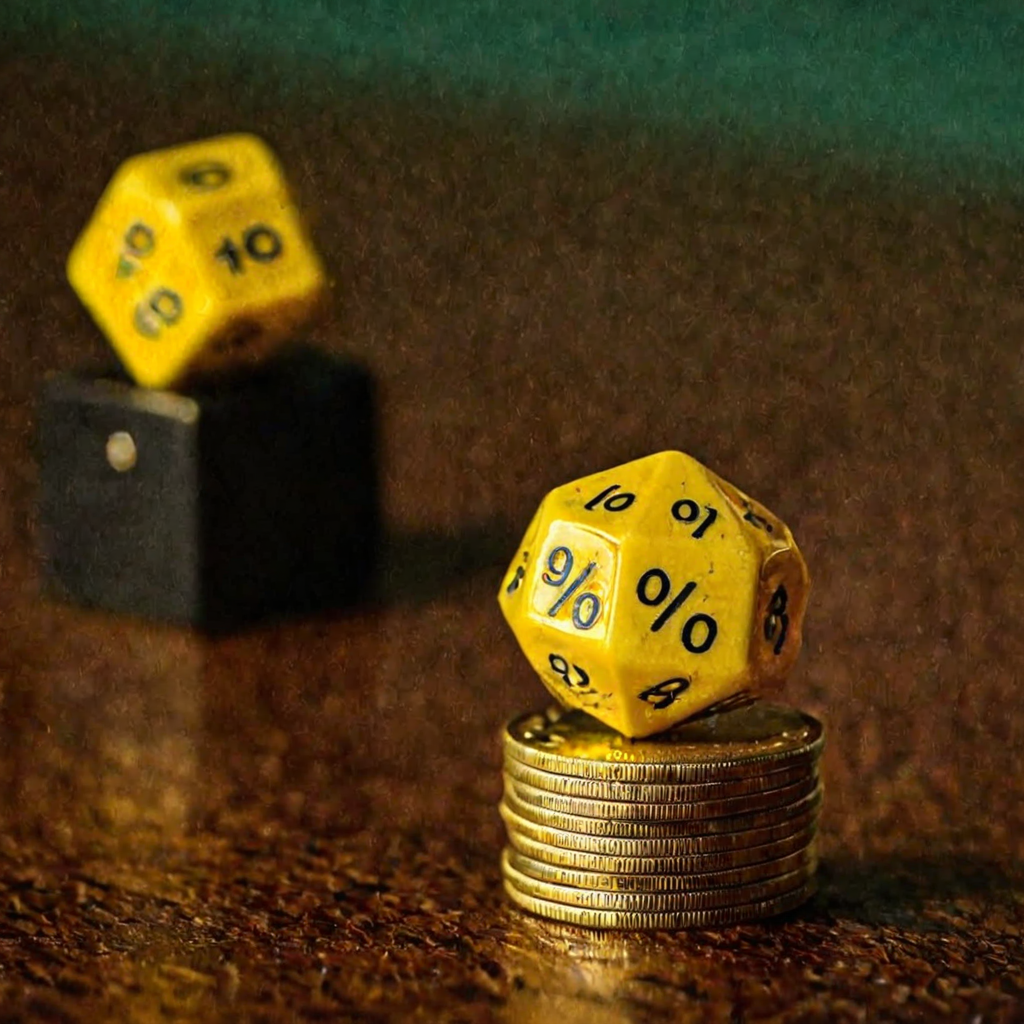
\includegraphics[scale=0.35]{0.Cover.png}}
    %\caption{Caption}
    %\label{fig:enter-label}
\end{figure}

\thispagestyle{empty} 
\end{titlepage}

\newpage
\pagecolor{white}
\tableofcontents
\newpage

\section{Concetti Base}
\subsection{Funzione Q}

In statistica, la funzione \(Q\), è la funzione di distribuzione della coda della funzione Gaussiana Standard.
In altre parole, \(Q(x)\) è la probabilità che una variabile aleatoria normale (gaussiana) ottenga un valore maggiore di  \(x\) derivazioni standard.
\begin{figure}[h]
\centering
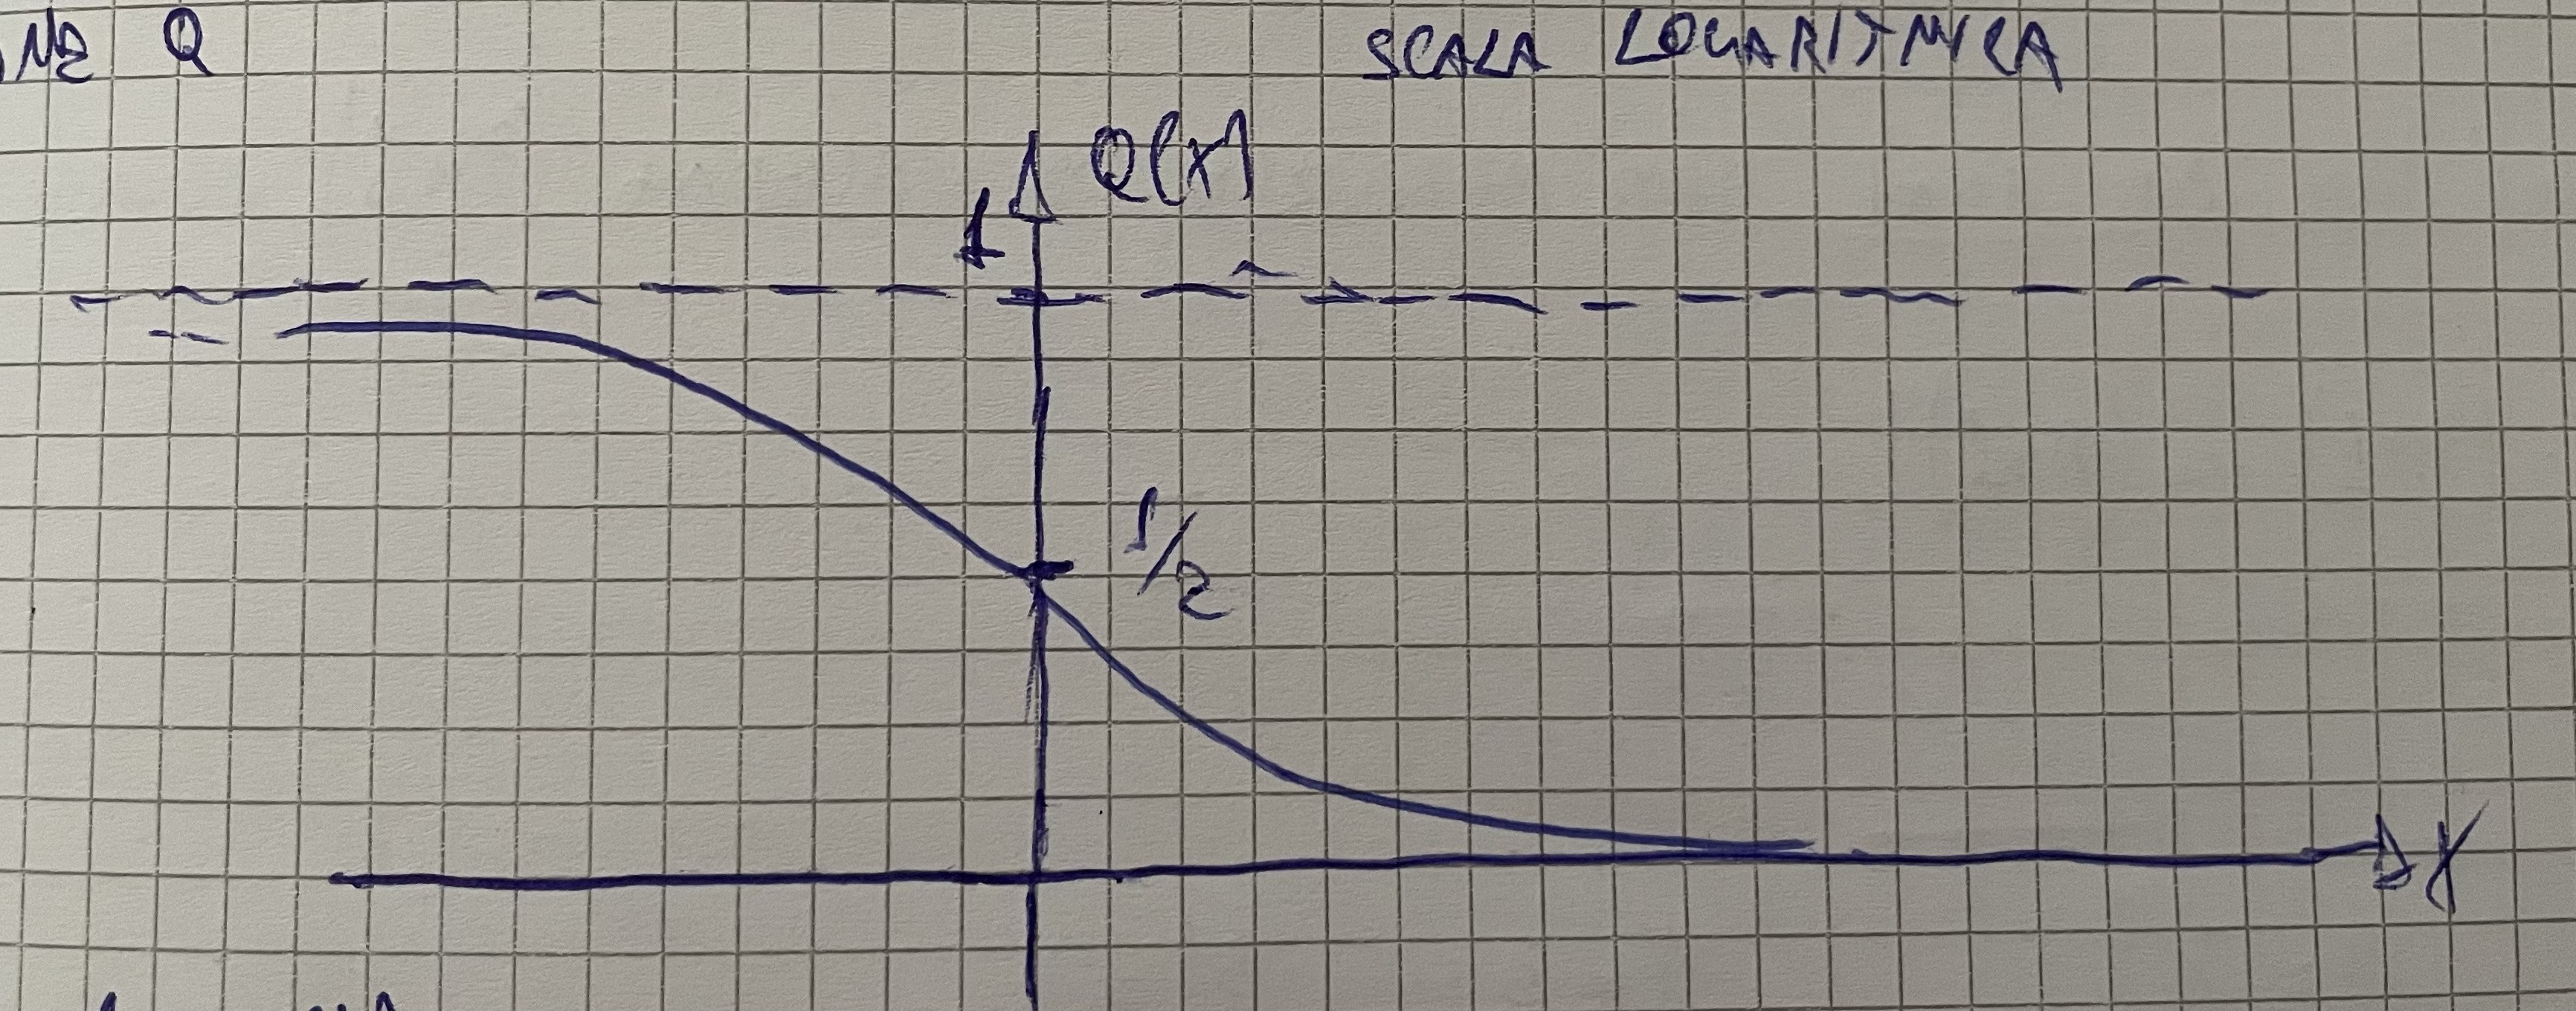
\includegraphics[scale=0.1]{1.Q1.jpeg}
\end{figure}

Equivalentemente \(Q(x)\) è la probabilità che una V.A. gaussiana standard assuma un valore maggiore di \(x\).
\begin{figure}[ht]
\centering
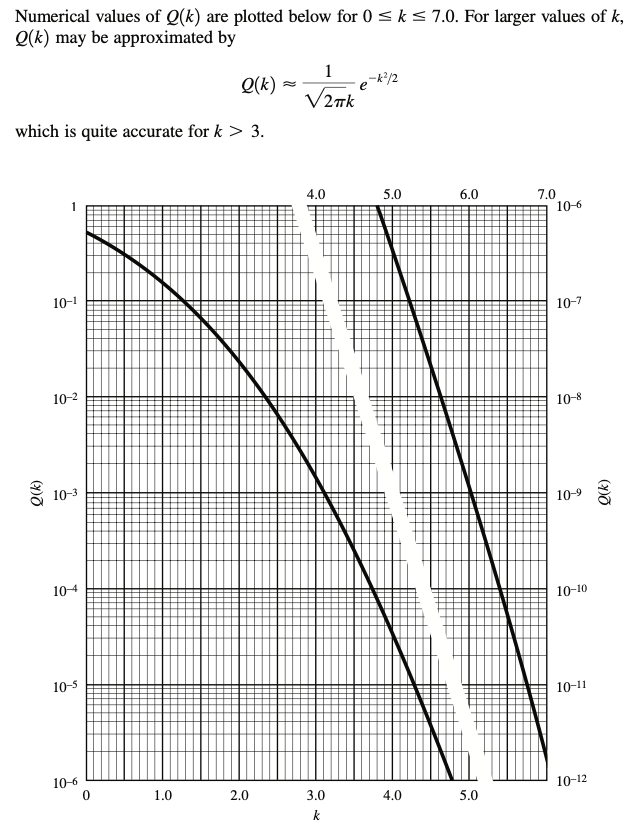
\includegraphics[scale=0.8]{2.Q2.png}
\end{figure}

La funzione \(Q\) è un concetto che verrà approfondito meglio più avanti negli appunti.

\subsection{Permutazioni}
Supponiamo di avere \(n\) oggetti: \(a_1,a_2,a_3, \dots, a_n\)
\\
\begin{tabular}{|p{13cm}}
La permutazione è il nome dell’operazione, ma anche il nome del risultato della suddetta operazione, ovvero il numero di combinazione/permutazioni di $n$ oggetti. 
\end{tabular}
\\
Quindi $P_n = n! = n \cdot (n-1) \cdot (n-2) \cdot \dots \cdot 2 \cdot 1$
\subsubsection{\underline{Esempio}}
$P_3 = 3 \cdot 2 \cdot 1 = 6$ \\
Esplicitando le varie permutazioni otteniamo: $\begin{matrix}

a_1 & a_2 & a_3 \\
a_1 & a_3 & a_2 \\
a_2 & a_1 & a_3 \\
a_2 & a_3 & a_1 \\
a_3 & a_1 & a_2 \\
a_3 & a_2 & a_1 \\

\end{matrix}$ \\ \\
\underline{\textsf{\textbf{-Dimostrazione(per induzione):}}} \\
\# Caso $n=1$ oggetti: $\implies$ $\implies P_1 = 1! = 1$ \\
\# Caso $n \rightarrow n+1$ supponiamo che $P_n = n!$ \\
Dobbiamo dimostrare che $P_{n+1} = (n+1)!$ \\
Aggiungendo un elemento alle permutazioni di $P_n$ otteniamo che ad ogni permutazione avremo $(n+1)$ nuove permutazioni: \\
$P_{n+1} = n! \cdot (n+1) = (n+1)!$ \\
\hspace*{0pt}\hfill $\square$
\subsubsection{\underline{Esempio}}
$n = 2 \implies 2! = 2$ 
Esplicitando le permutazioni otteniamo: $\begin{matrix}
\#1 & a_1 & a_2 \\
\#2 & a_2 & a_1
\end{matrix}$ 
\\
\subsubsection{\underline{Esempio}}
$n = 3 \implies 3! = 6$ 
Esplicitando le permutazioni otteniamo: $\begin{matrix}

\#1 & \underline{a_3} & a_1 & a_2 \\
& a_1 & \underline{a_3} & a_2 \\
& a_1 & a_2 & \underline{a_3} \\

\#2 & \underline{a_3} & a_2 & a_1\\
& a_2 & \underline{a_3} & a_1 \\
& a_2 & a_1 & \underline{a_3} \\

\end{matrix}$ \\


\subsection{Disposizioni(di n oggetti presi k alla volta)}

\begin{tabular}{|p{13cm}}
Le disposizioni sono sequenze ordinate di $k$ oggetti estratti dagli $n$ totali. \\
(Nelle disposizioni l’ordine degli oggetti è molto importante).
\end{tabular}
\\
$D_{n,k} = \frac{n!}{(n-k)!}$
\\
\subsubsection{\underline{Dimostrazione}}
Molto utile ai fini di questa dimostrazione il seguente grafico ad albero: 
\begin{figure}[h]
\centering
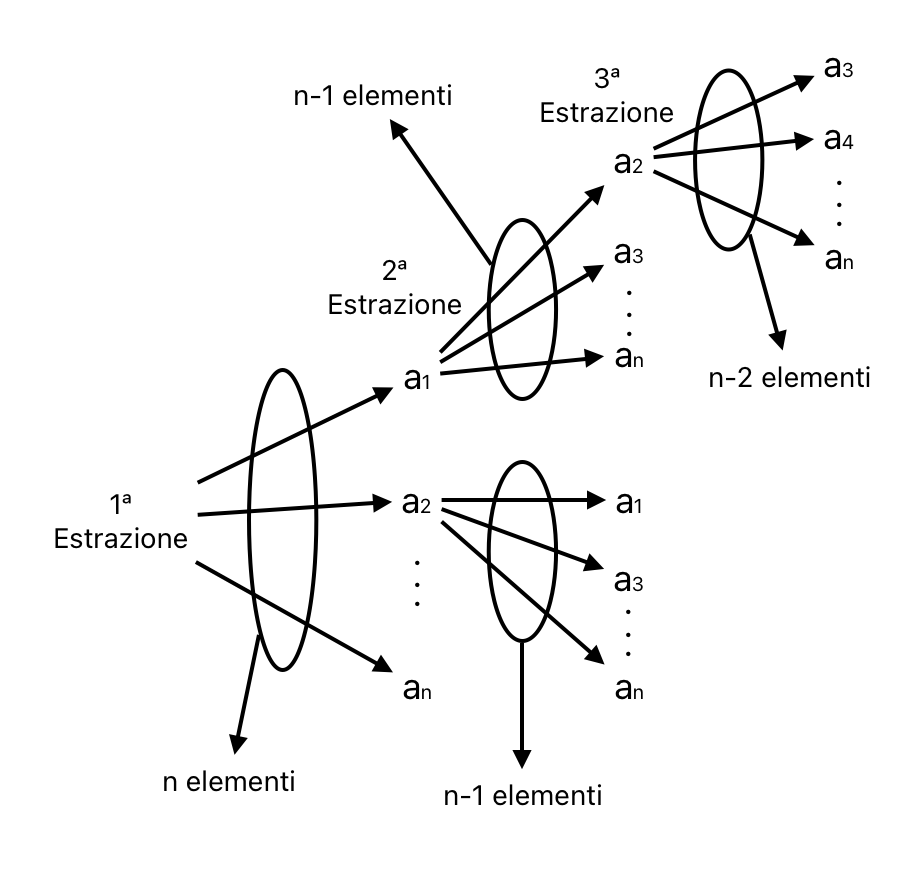
\includegraphics[scale=0.45]{3.Dispo1.png}
\end{figure} \\
Che possiamo "tradurre" come:
\begin{center}
    $D_{n,k} = \frac{n \cdot (n-1) \cdot (n-2) \cdot \dots \cdot(n-k+1) \cdot (n-k) \cdot (n-k-1) \cdot \dots \cdot 2 \cdot 1}{(n-k) \cdot (n-k-1) \cdot \dots \cdot 2 \cdot 1}$
\end{center}
\hspace*{0pt}\hfill $\square$ \\
\subsubsection{\underline{Esempio}}
3 oggetti presi 2 alla volta:
\begin{figure}[h]
\centering
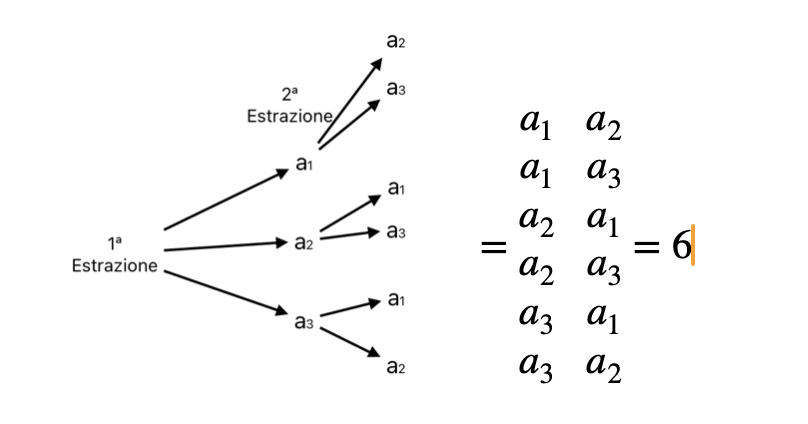
\includegraphics[scale=0.5]{4.Dispo2.png}
\end{figure} \\
$D_{3,2} = \frac{3!}{(3-2)!} = \frac{6}{1} = 6$
\subsection{Disposizioni con ripetizione}
$D^{(R)}_{n,k} = n^k$ 
\subsubsection{\underline{Esempio}}
Tutti i numeri con 3 cifre: $\begin{matrix}

000 \\
001 \\
002 \\
\vdots \\
999

\end{matrix}$ \\
\\
Quindi il numero di cifre (oggetti) è: $n=10$ e le prendiamo $k=3$ alla volta. \\
Di conseguenza otteniamo: $D_{10,3}^{(R)} = 10^3 = 1000$

\subsection{Combinazioni}

\begin{tabular}{|p{14cm}}
Sono sequenze non ordinate di $k$ oggetti estratti dagli $n$ totali. \\
(Al contrario delle disposizioni, nelle combinazioni, l’ordine degli oggetti non è importante).
\end{tabular}
\\
$C_{n,k} = \left( \begin{matrix} n \\ k \end{matrix} \right) = \frac{n!}{k! \cdot (n-k)!}$
\subsubsection{\underline{Casi Particolari}}
\begin{enumerate}
    \item $C_{n,k} \cdot k! = \frac{n!}{\cancel{k!} \cdot (n-k)!} \cdot \cancel{k!} =D_{n,k}$
    \item $C_{n,k} = \frac{D_{n,k}}{k!} = \frac{n!}{(n-k)! \cdot k!} = \left( \begin{matrix} n \\ k \end{matrix} \right)$
\end{enumerate} 
\newpage
\subsubsection{\underline{Esempio}}
$n=3$ e $k=2$ \\
\begin{figure}[h]
\centering
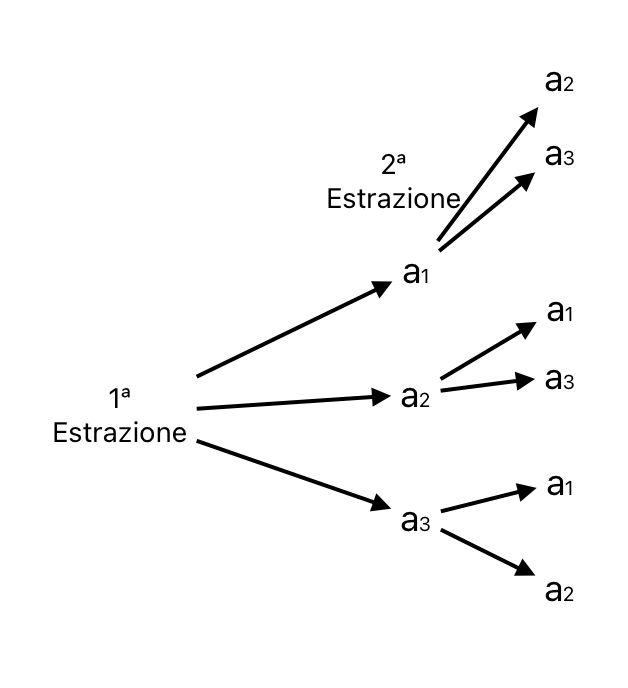
\includegraphics[scale=0.5]{5.Comb.png}
\end{figure} \\
Dall'immagine qua sopra possiamo capire che: $\begin{matrix}
a_1 & a_2 = a_2 & a_1 \\
a_1 & a_3 = a_3 & a_1 \\
a_2 & a_3 = a_3 & a_2 \\
\end{matrix} 
\Biggr\}
=3$ \\
$C_{3,2} = \left( \begin{matrix} 3 \\ 2 \end{matrix} \right) =  \frac{3!}{2! \cdot (3-2)!} = \frac{6}{2} = 3$
\section{Funzioni Essenziali}
\subsection{Funzione Gaussiana Standard(Normale)}
$g(t) = \frac{1}{\sqrt{2 \pi}} \cdot e^{-\frac{t^2}{2}}$

\subsubsection{\underline{Alcuni valori noti}}
\begin{enumerate}
    \item $g(1) = g(-1) \simeq \frac{1}{\sqrt{2 \pi}}\cdot 0,6$
    \item $g(2) = g(-2) \simeq \frac{1}{\sqrt{2 \pi}}\cdot 0,136$
\end{enumerate}
\subsubsection{\underline{Grafico}}
\begin{figure}[ht]
\centering
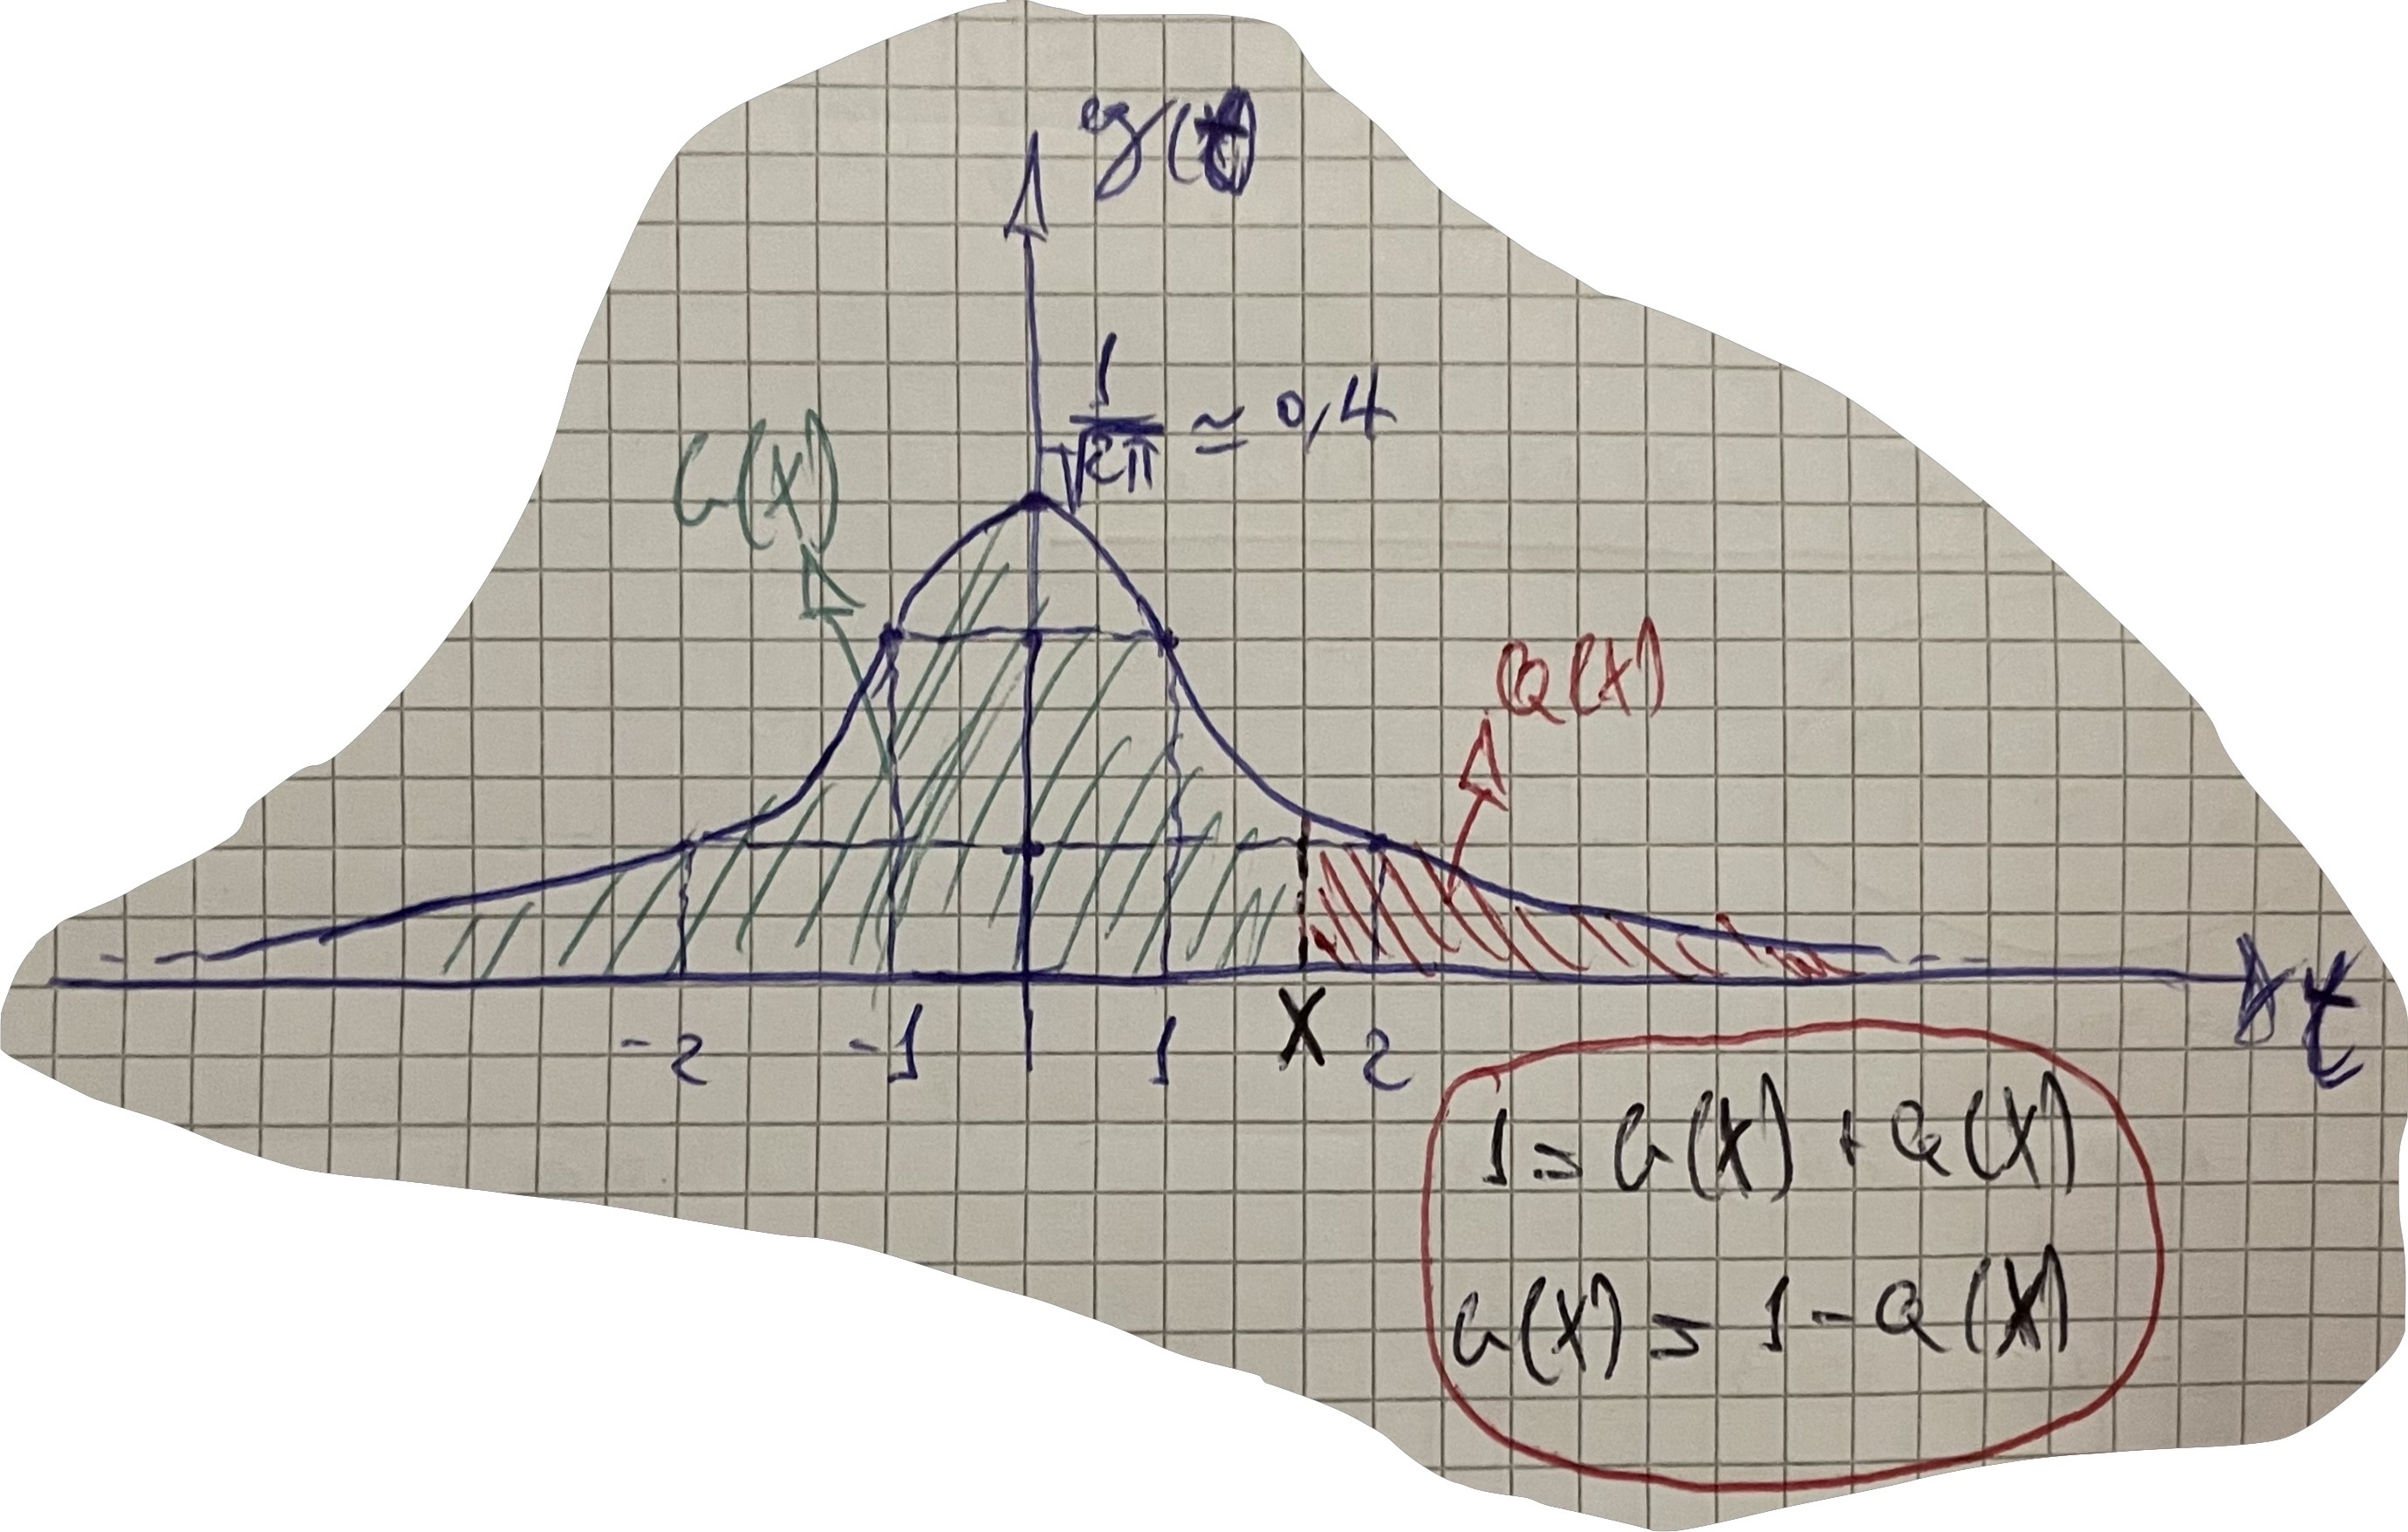
\includegraphics[scale=0.13]{6.Gauss.jpeg}
\end{figure} 
\newpage
\subsection{Funzione Gaussiana Generica}
$f(t) = \frac{1}{\sqrt{2 \pi \sigma^2}} \cdot e^{-\frac{(t- \eta)^2}{2 \sigma^2}}$ dove $\eta \text{(Eta)} \in \mathbb{R}$ e $\sigma^2\text{(Sigma)} > 0$
\subsubsection{\underline{Grafico}}
\begin{figure}[ht]
\centering
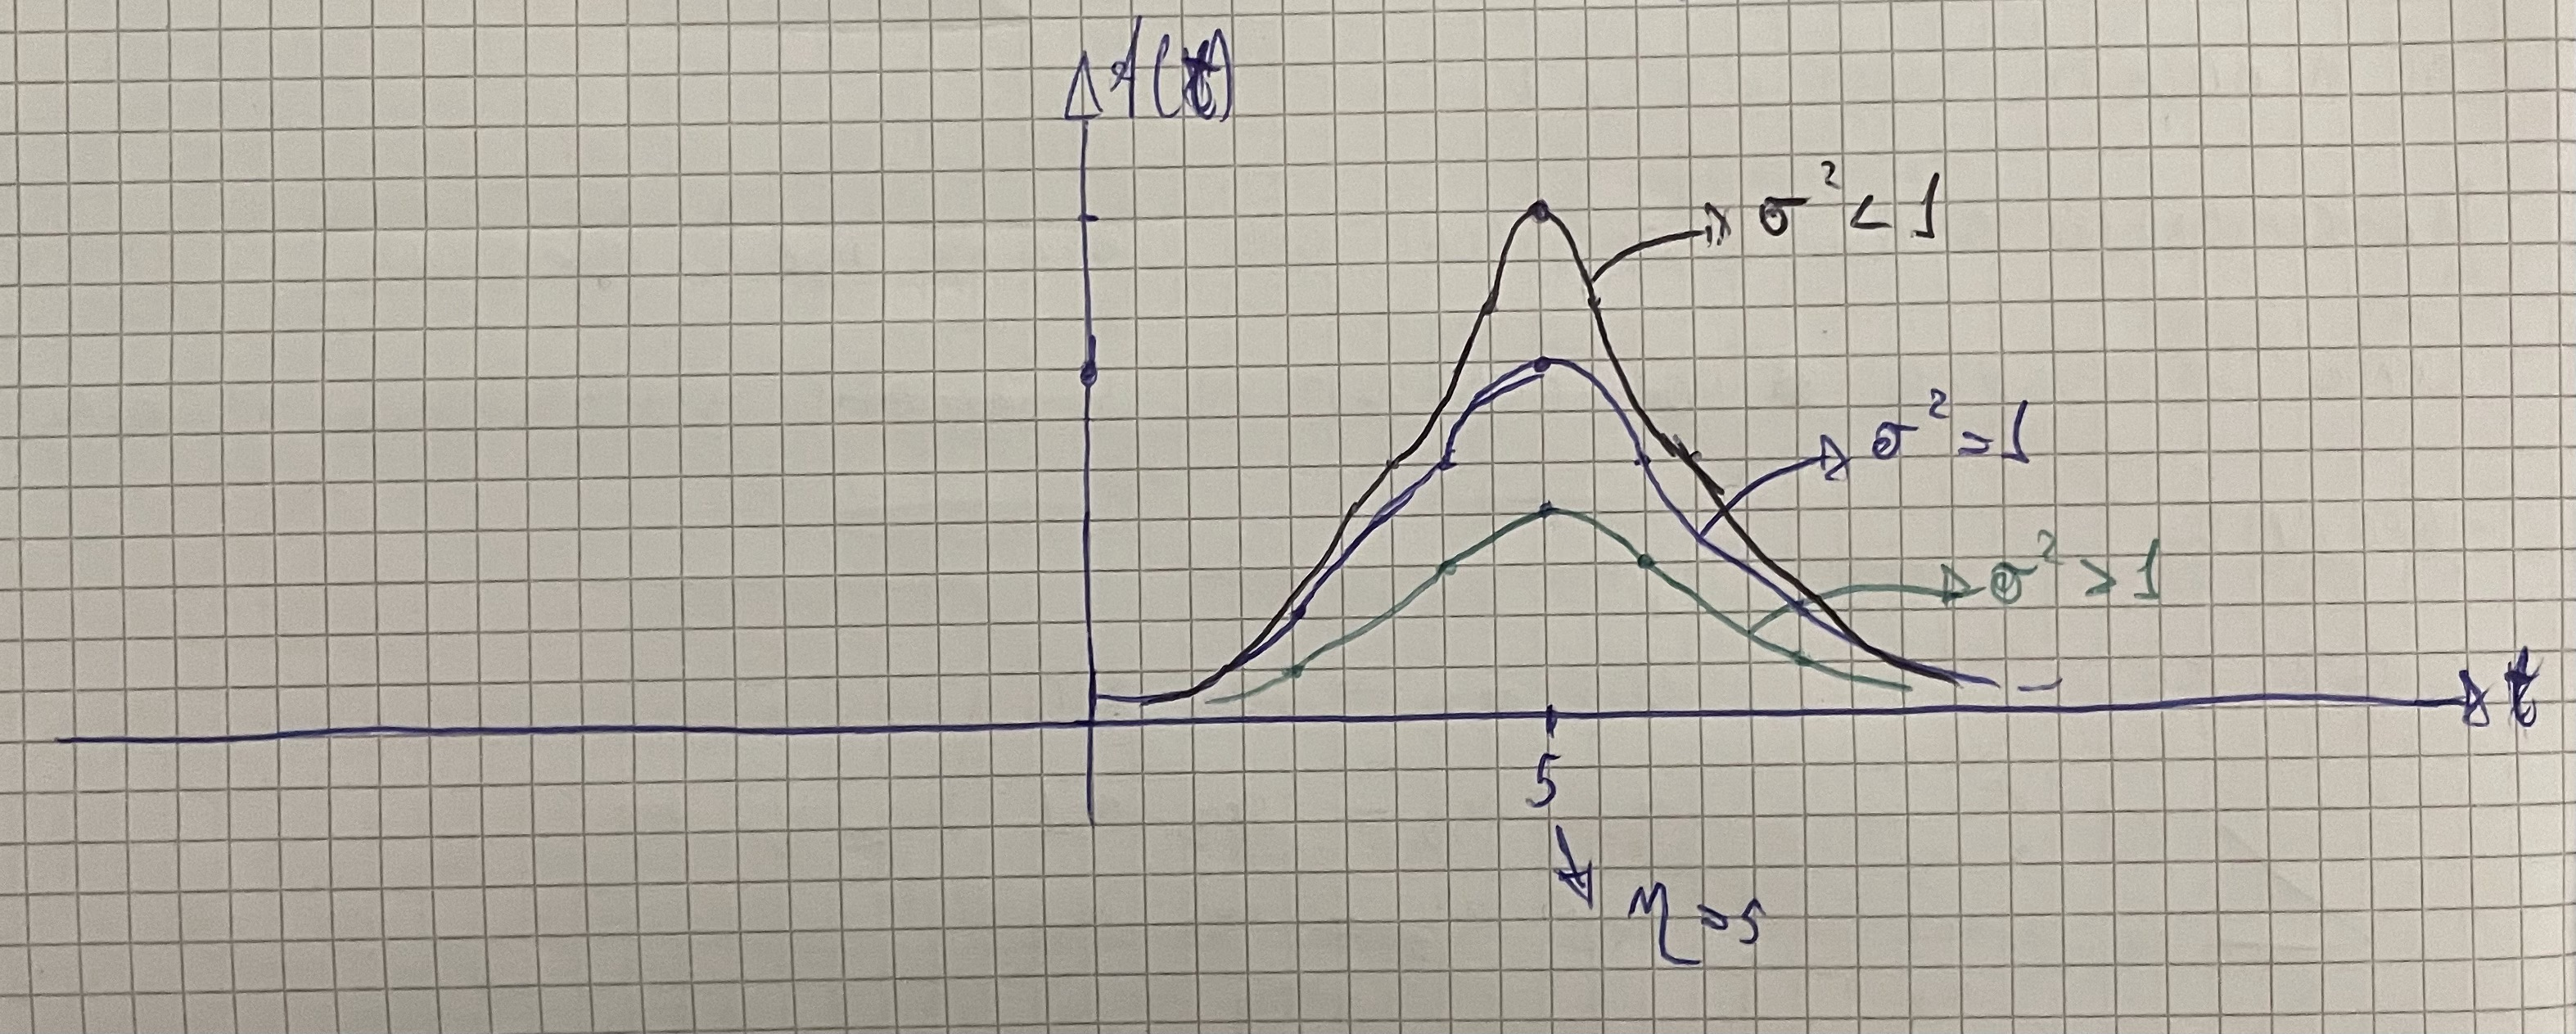
\includegraphics[scale=0.15]{7.Gauss2.jpeg}
\end{figure}

\subsection{Aree delle Funzioni Gaussiane}
\begin{enumerate}
    \item Gaussiana Standard: $\int_{\infty}^{+\infty}g(t)dt=1$
    \item Gaussiana Generica : $\int_{-\infty}^{+\infty}f(t)dt=1$
\end{enumerate} 
Da questo possiamo dedurre che le funzioni gaussiane hanno area unitaria.

\subsection{Primitive della Gaussiana Standard}
\begin{itemize}
    \item $G(x)=\int_{-\infty}^{+x}g(t)dt=\frac1{2\pi}\int_{-\infty}^{+x}e^{-\frac{t^2}2}dt$
    \item $Q(x)=\int_{-x}^{+\infty}g(t)dt=\frac1{2\pi}\int_{-x}^{+\infty}e^{-\frac{t^2}2}dt$
\end{itemize} 
Come possiamo notare questa è la funzione Q di cui abbiamo parlato
all'inizio.
\subsubsection{\underline{Grafico}}
\begin{figure}[ht]
\centering
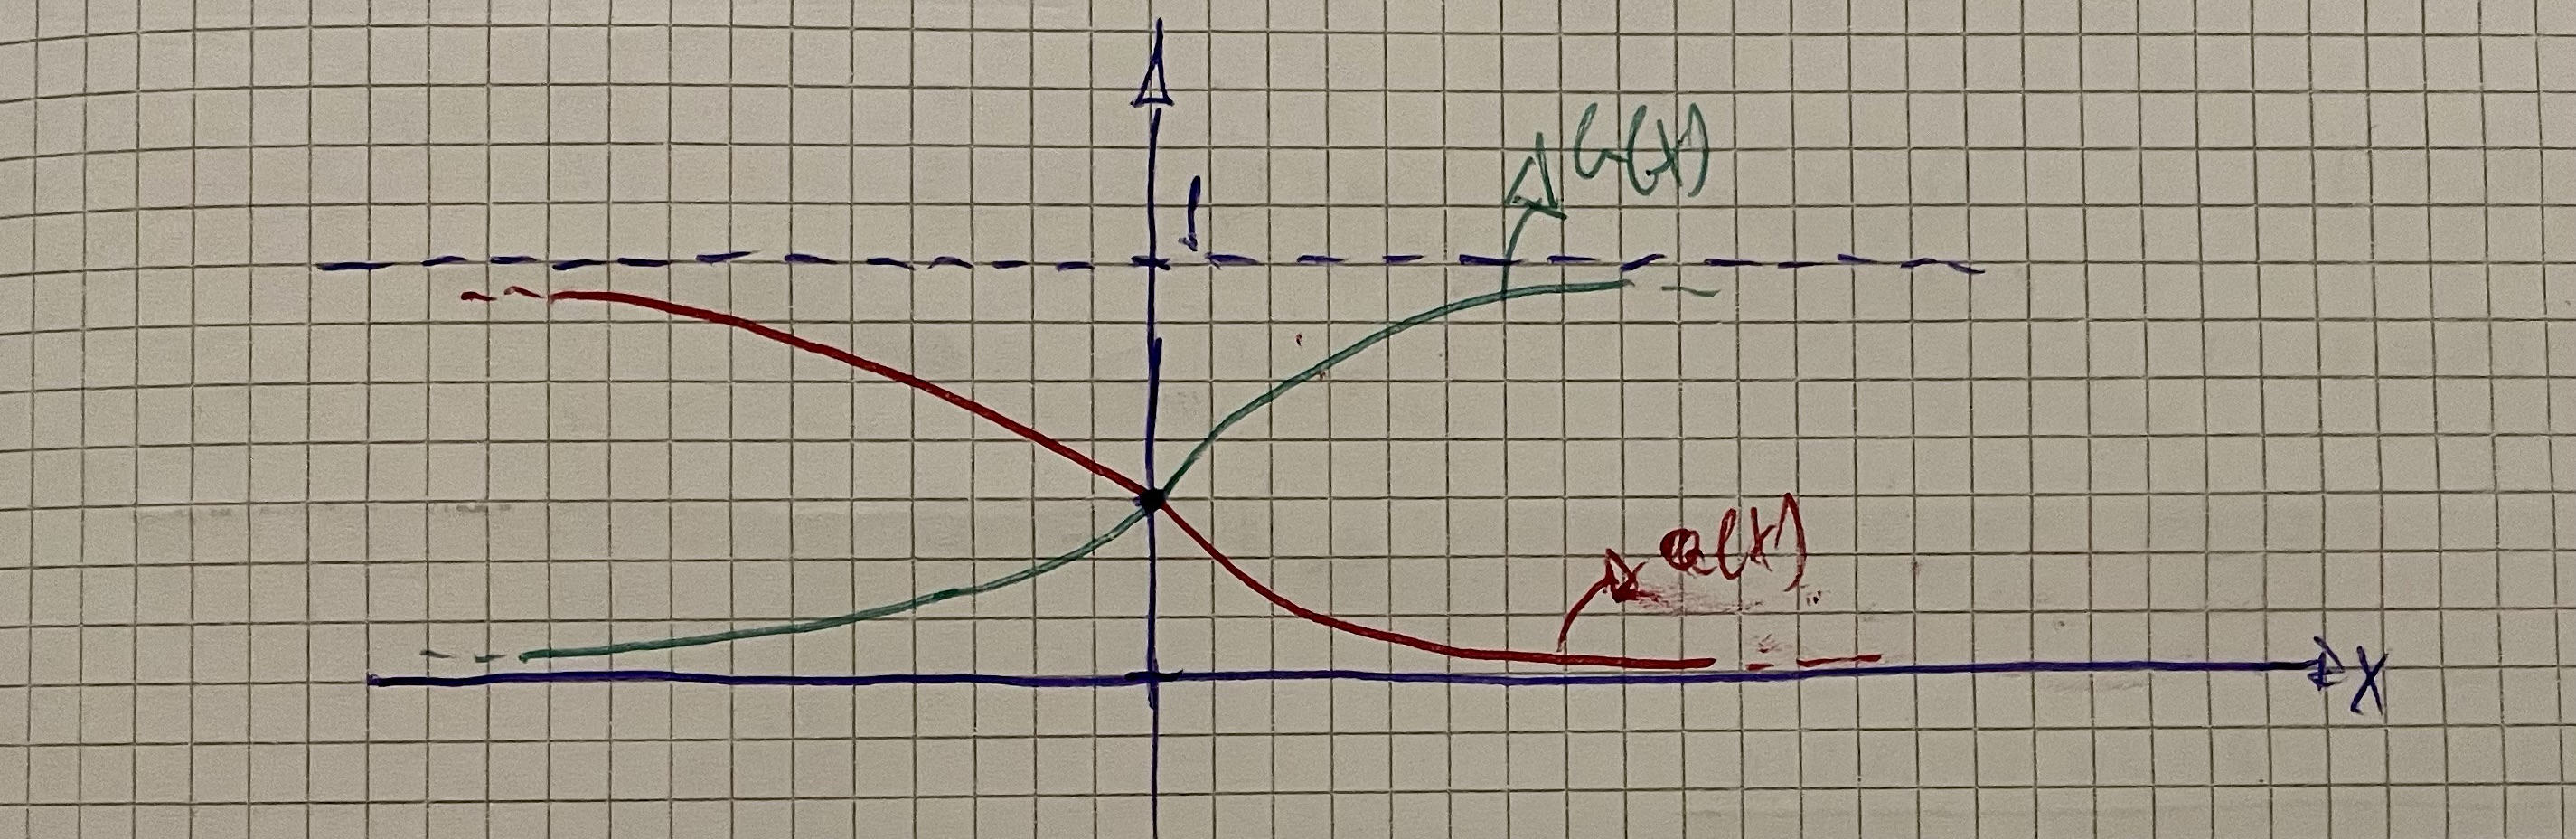
\includegraphics[scale=0.15]{images/8.Q_G.jpeg}
\end{figure} ~\\
La funzione Q sarà molto utile per calcolare altri integrali.
\subsubsection{\underline{Esempio}}
$\int_{x_1}^{x_2} f(x) dx = \frac{1}{\sqrt{2 \pi \sigma^2}} \int_{x_1}^{x_2} e^{-\frac{(x - \eta)^2}{2 \sigma^2}} dx =
\frac{1}{\sqrt{2 \pi \sigma^2}} \int_{x_1}^{x_2} e^{-\frac12 \frac{(x - \eta)^2}{\sigma^2}} dx =
\frac{1}{\sqrt{2 \pi \sigma^2}} \int_{x_1}^{x_2} e^{-\frac12 \left( \frac{(x - \eta)}{\sigma} \right)^2 }  dx$ \\
Eseguiamo un cambio di variabile: $\frac{x - \eta}{\sigma} = z$ e quindi $\frac{dx}{\sigma} = dz$ \\
$= \frac{1}{\sqrt{2 \pi }} \int_{\frac{x_1 - \eta }{\sigma}}^{\frac{x_2 - \eta }{\sigma}} e^{- \frac{z^2}{2} } dz =
1 - {\color{red} \frac{1}{\sqrt{2 \pi }} \int_{\frac{x_2 - \eta }{\sigma}}^{+\infty} e^{- \frac{z^2}{2} } dz} 
- {\color{blue} \frac{1}{\sqrt{2 \pi }} \int_{- \infty}^{\frac{x_1 - \eta }{\sigma}} e^{- \frac{z^2}{2} } dz}$ \\
$ = {\color{green}\underline 1}  {\color{red} -Q\left( \frac{x_2 - \eta}{\sigma} \right) } {\color{green}\underline{ {\color{blue} -G\left( \frac{x_1 - \eta}{\sigma} \right) }}}
= {\color{red} -Q\left( \frac{x_2 - \eta}{\sigma} \right) } {\color{green} +Q\left( \frac{x_1 - \eta}{\sigma} \right) } $ \\
$= +Q\left( \frac{x_1 - \eta}{\sigma} \right)   -Q\left( \frac{x_2 - \eta}{\sigma} \right) $

\subsection{Valori Noti della Funzione Q}
\begin{table} [h]
    \centering
    \begin{tabular}{|c|c|c|}
    \hline
        $Q(-\infty) = 1$ & $Q(0) = 0.5 $ & $Q(+1) = 0.16$\\
        \hline 
        $Q(-2) = 0.98$ &  & $Q(+2) = 0.02$\\
        \hline 
        $Q(-1) = 0.84$&  & $Q(+\infty) = 0$\\
    \hline
    \end{tabular}
\end{table}

\subsection{Funzione Gradino Unitario}
Definiamo la funzione gradino unitario come: $u(t) = \begin{cases} 
1 & \text{se } t \geq 0 \\
0 & \text{se } t < 0 \\
\end{cases}$
\subsubsection{\underline{Grafico}}
\begin{figure}[ht]
\centering
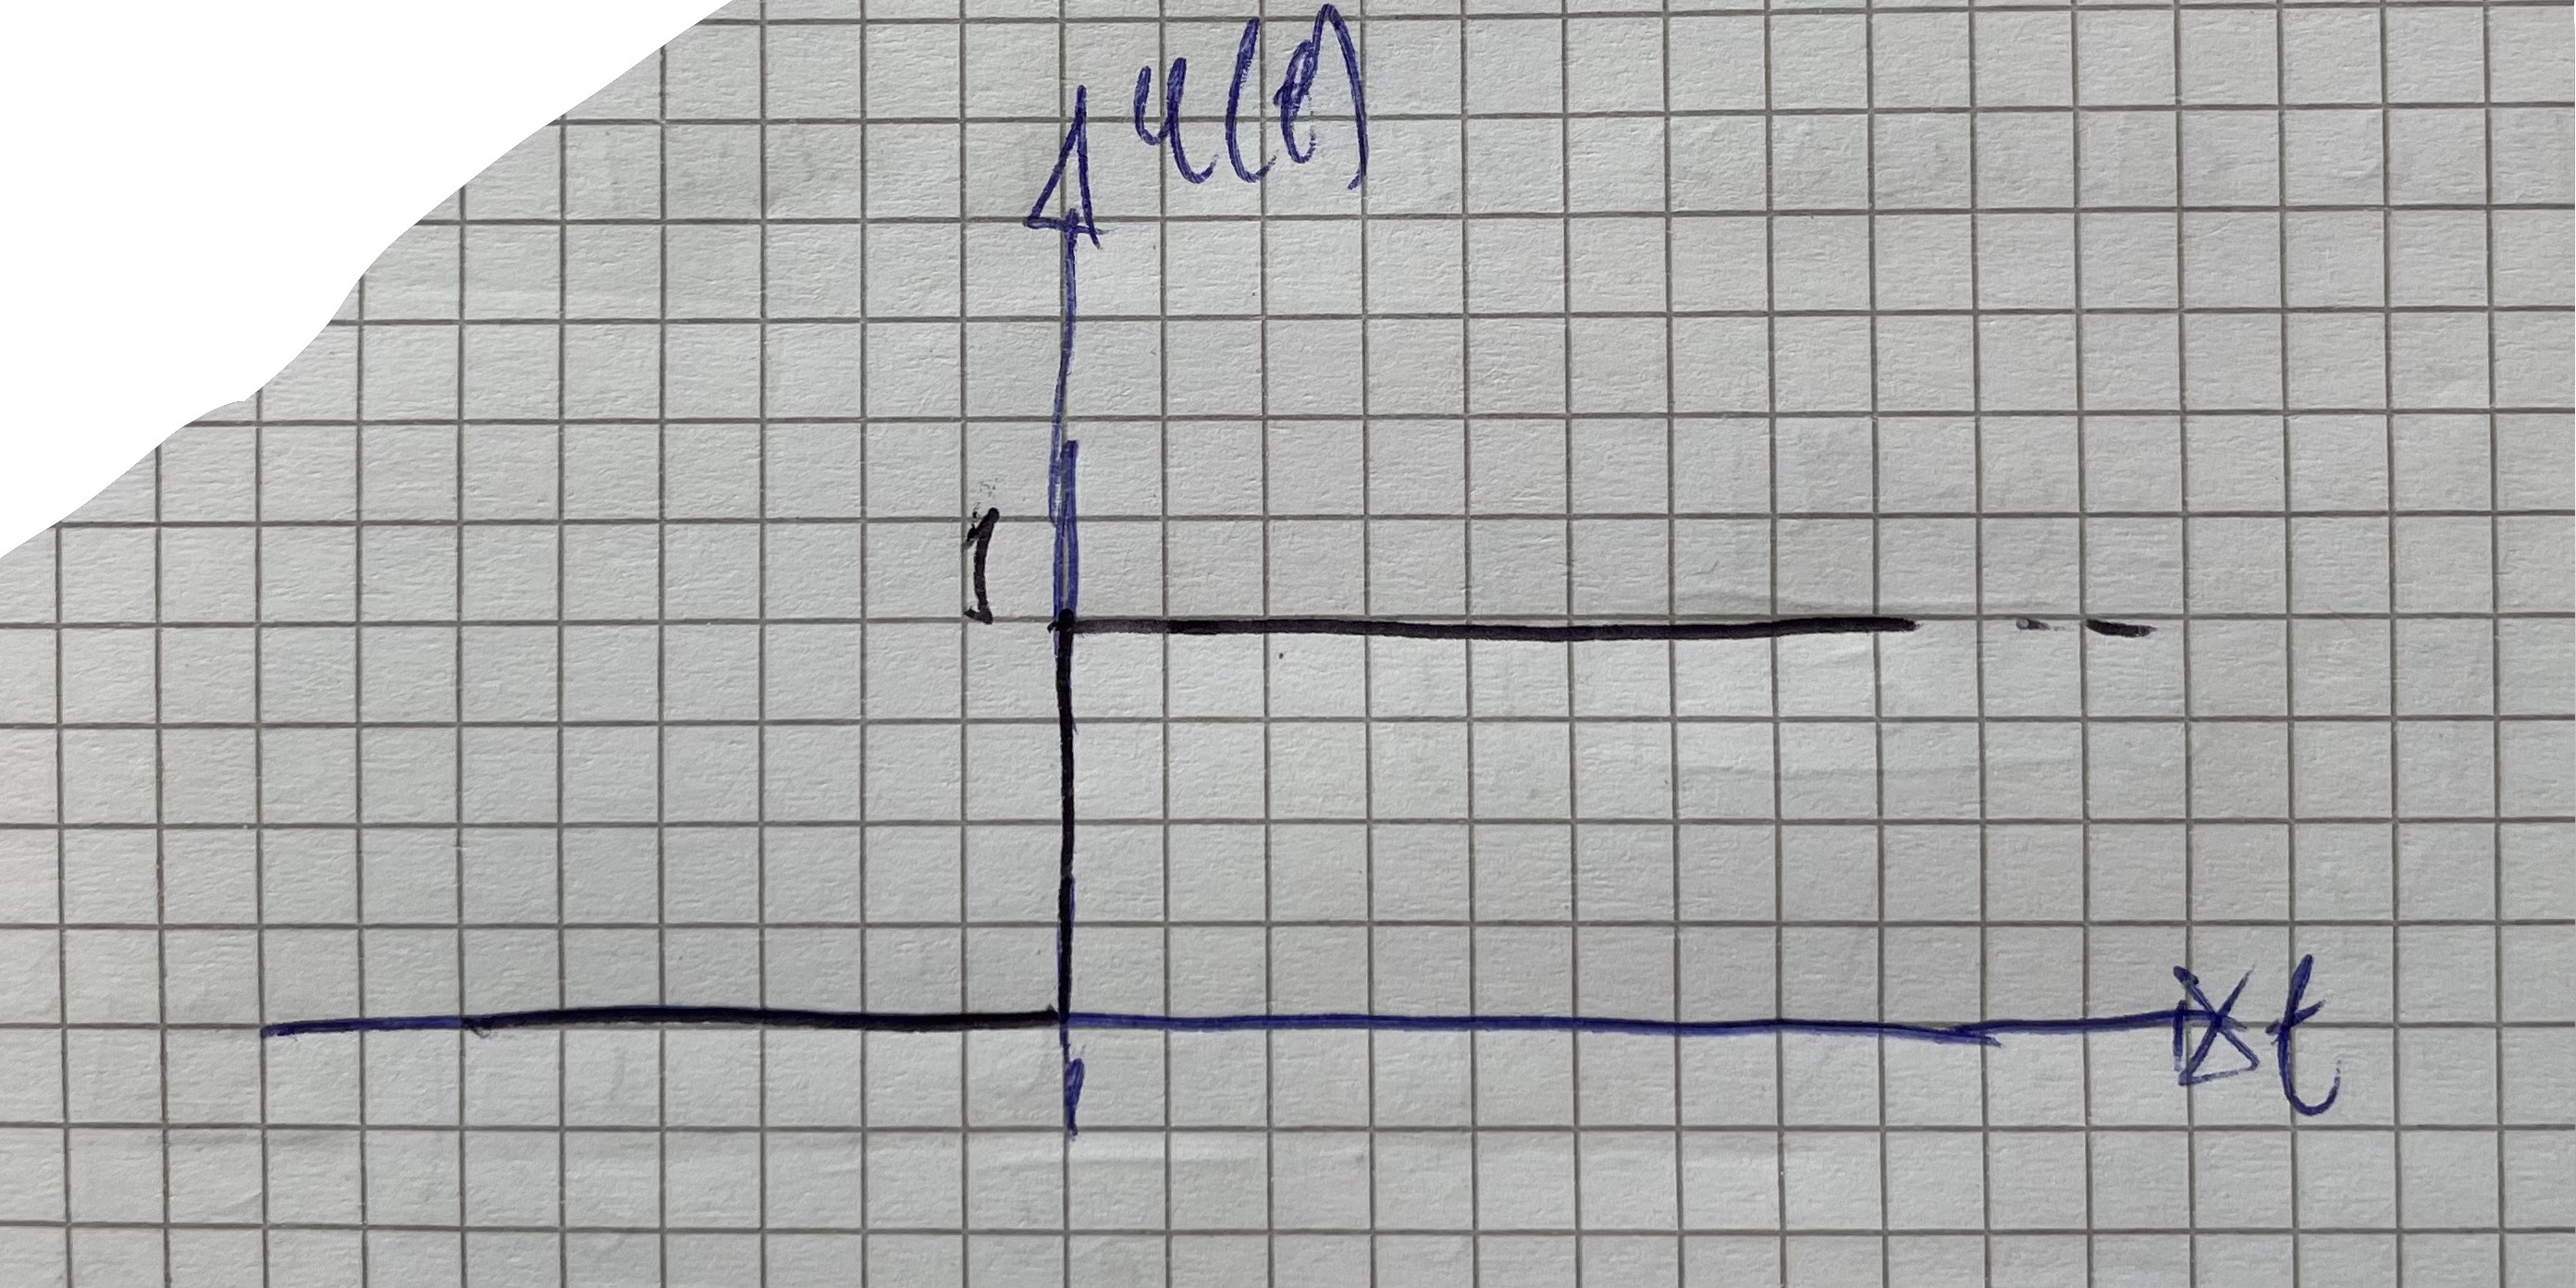
\includegraphics[scale=0.13]{images/9.GradUni.jpeg}
\end{figure}

\subsection{Funzione Impulso Rettangolare}
Definiamo la funzione impulso rettangolare come: $\Pi(t) = \begin{cases} 
1 & \text{se } |t| \leq 0 \\
0 & \text{se } |t| > 0 \\
\end{cases}$
\newpage
\subsubsection{\underline{Grafico}} ~\\
\begin{figure}[ht]
  \begin{subfigure}{.5\textwidth}
  \centering
    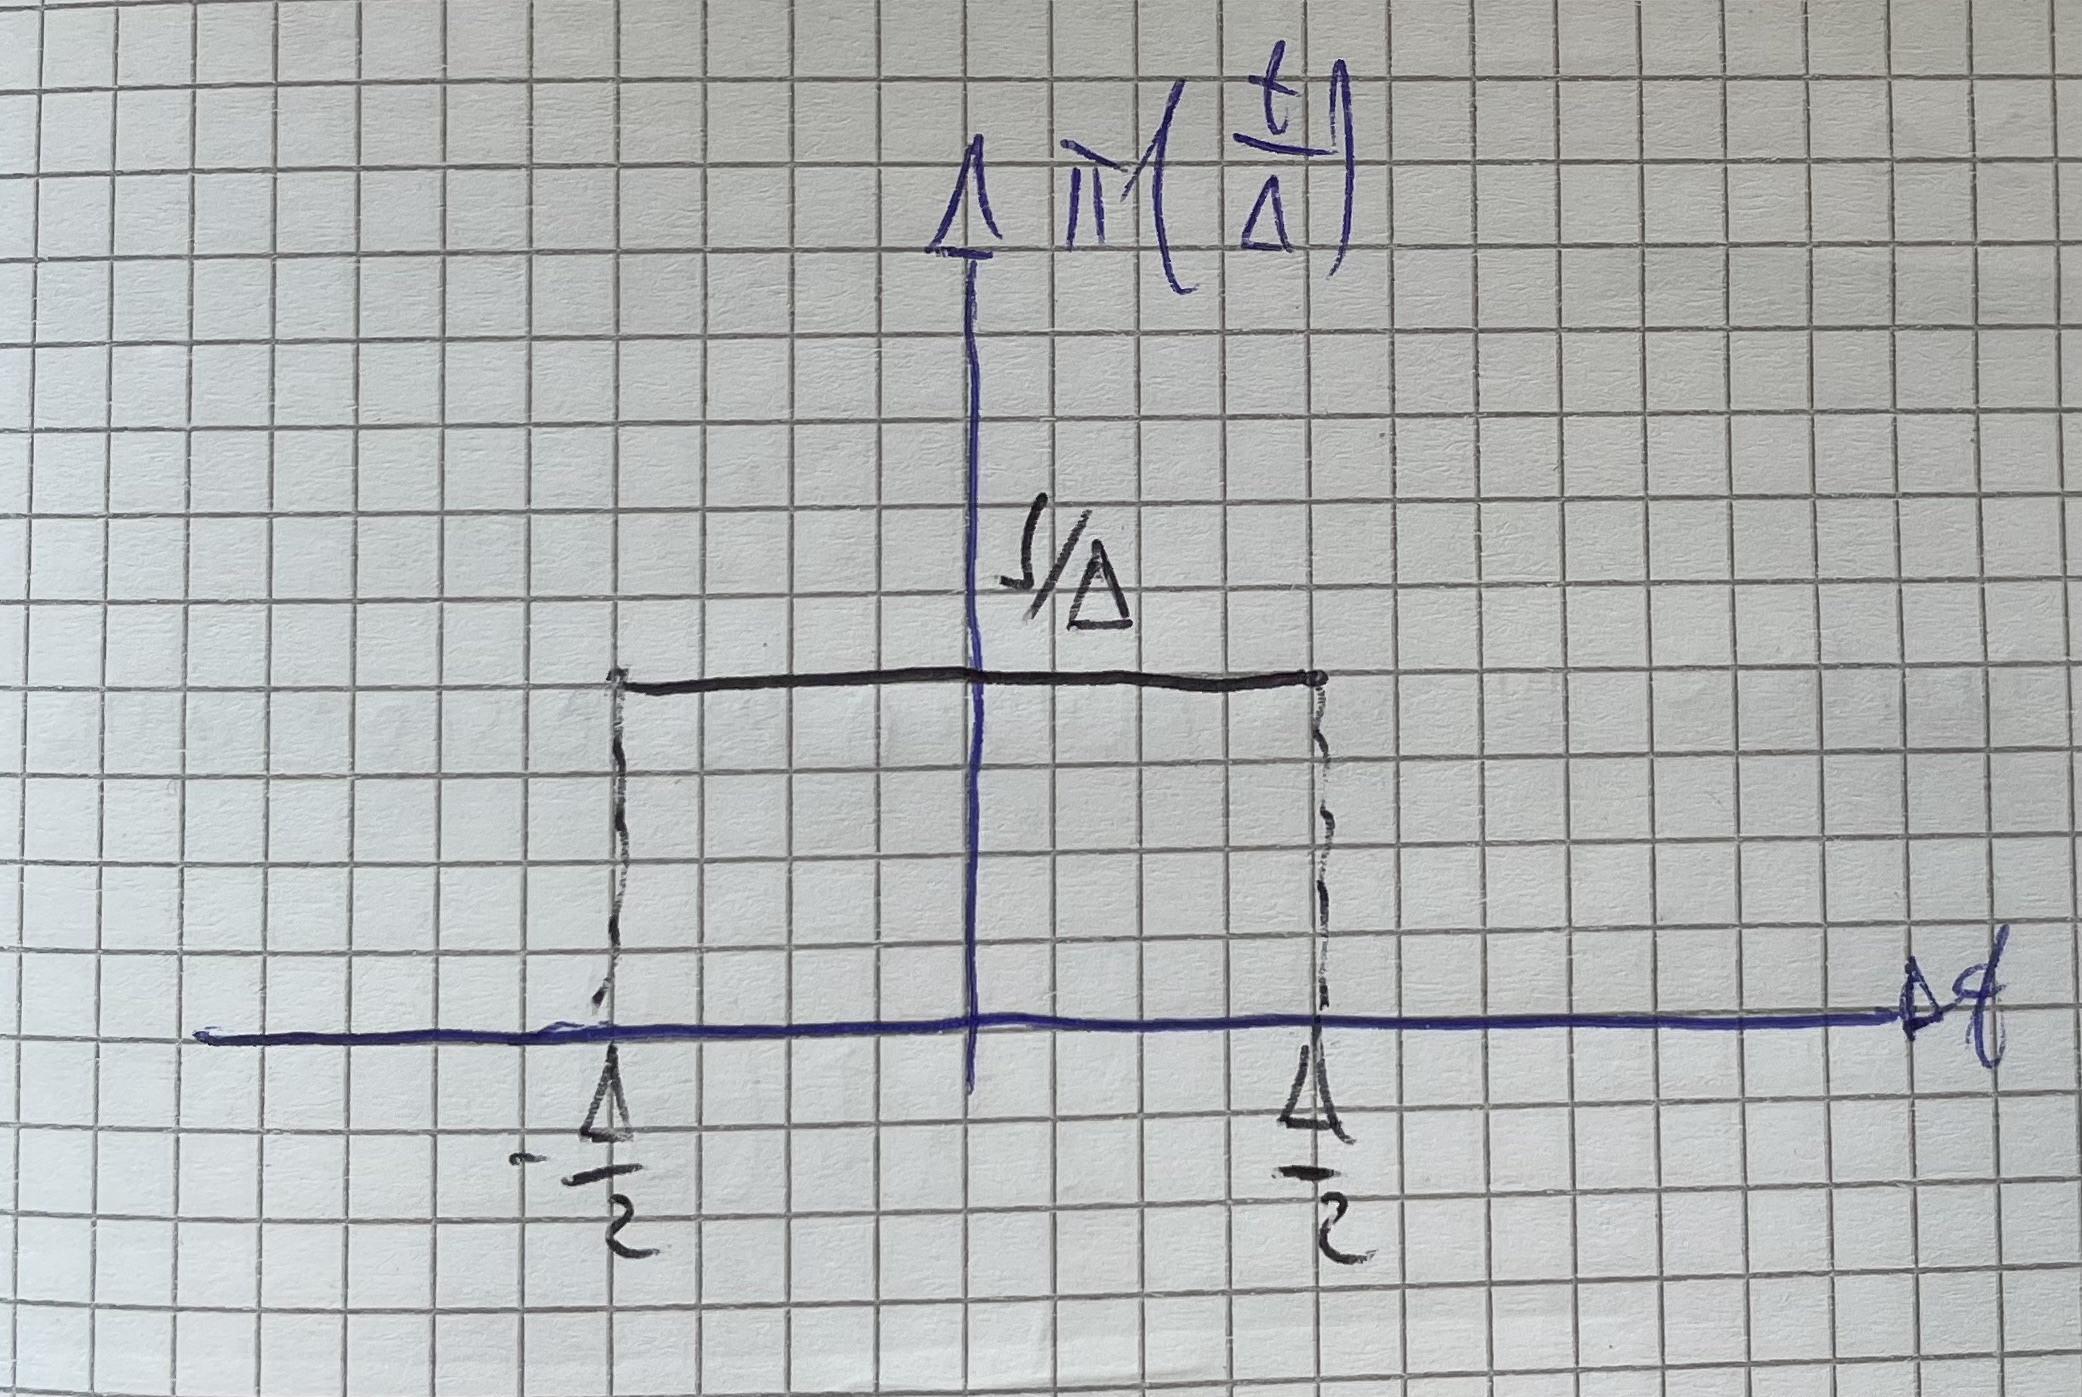
\includegraphics[width=.9\linewidth]{images/10.Rett1.jpeg}
    %\caption{}
  \end{subfigure}
  \begin{subfigure}{.5\textwidth}
  \centering
    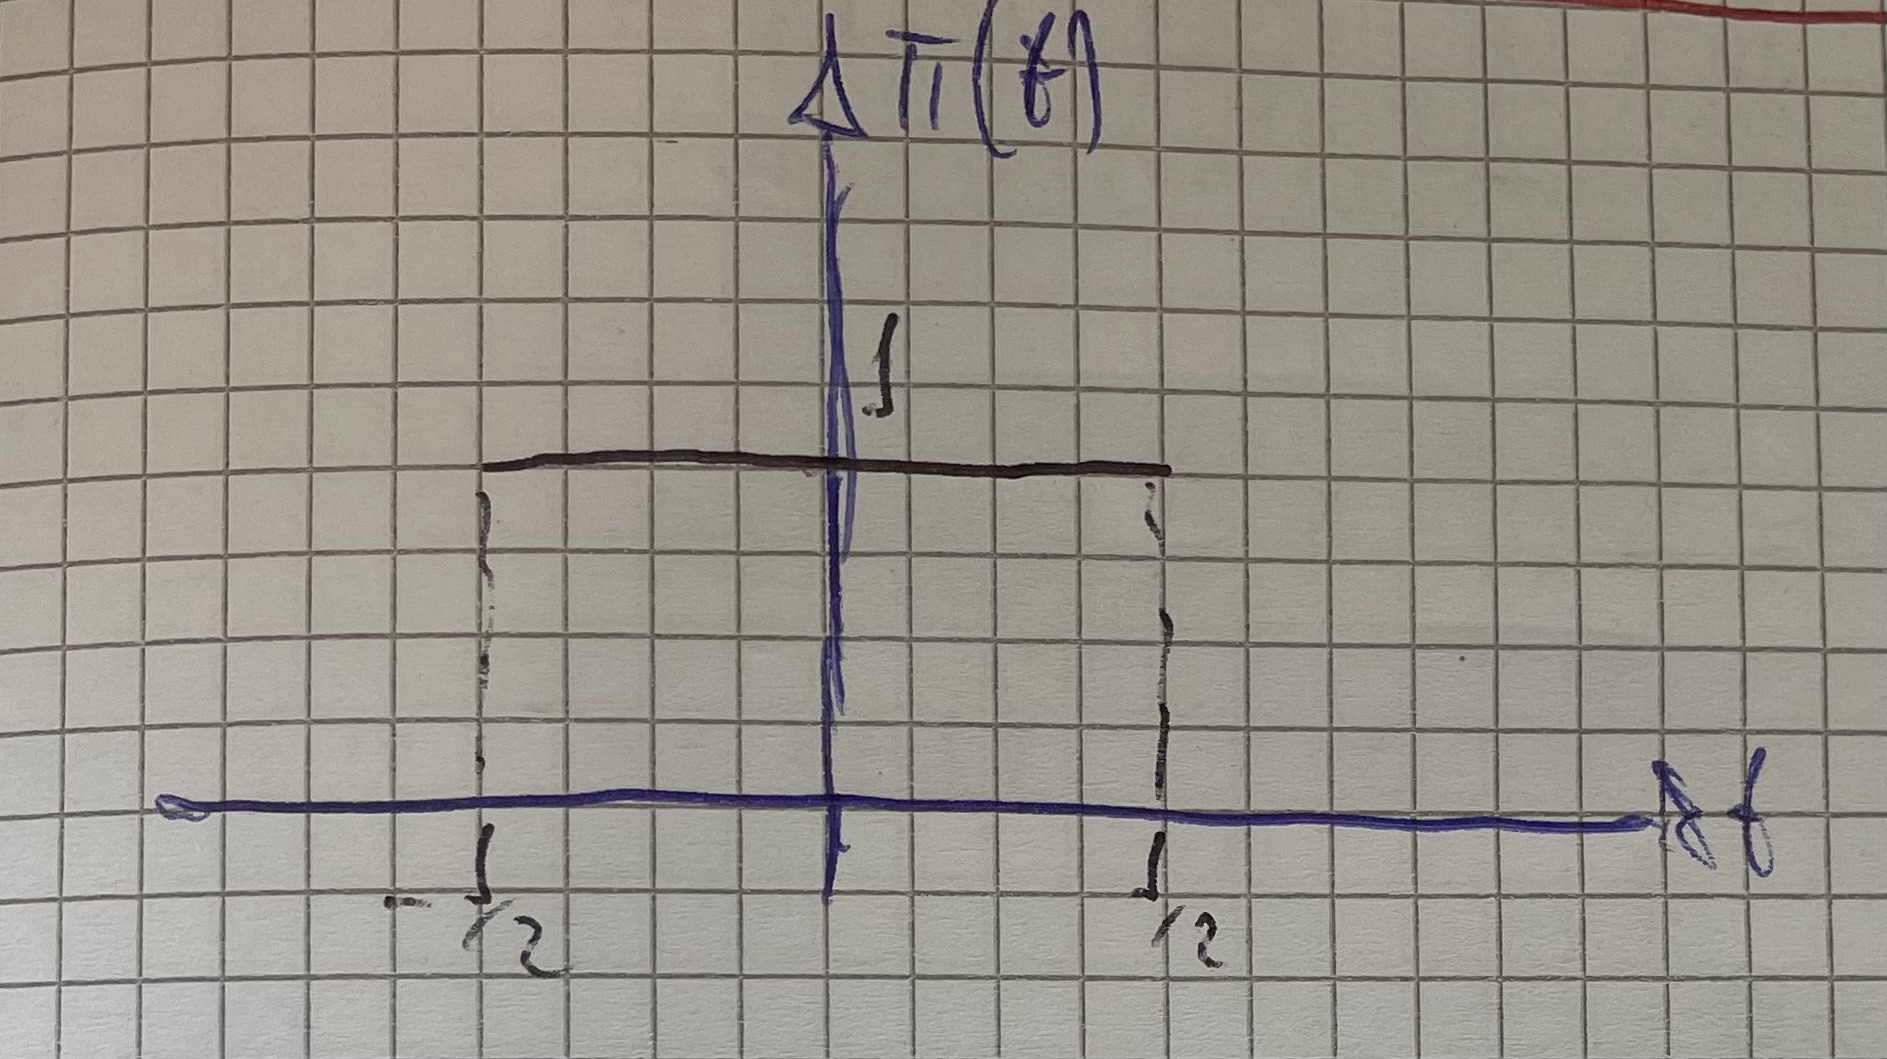
\includegraphics[width=.9\linewidth]{images/11.Rett2.jpeg}
    %\caption{}
  \end{subfigure}
  %\caption{}
\end{figure} 

\subsection{Funzione Impulsiva di Dirac (Delta di Dirac)}
Definiamo la funzione impulsiva di Dirac come: $\delta(t)$
\subsubsection{\underline{Grafico}} ~\\
\begin{figure}[ht]
\centering
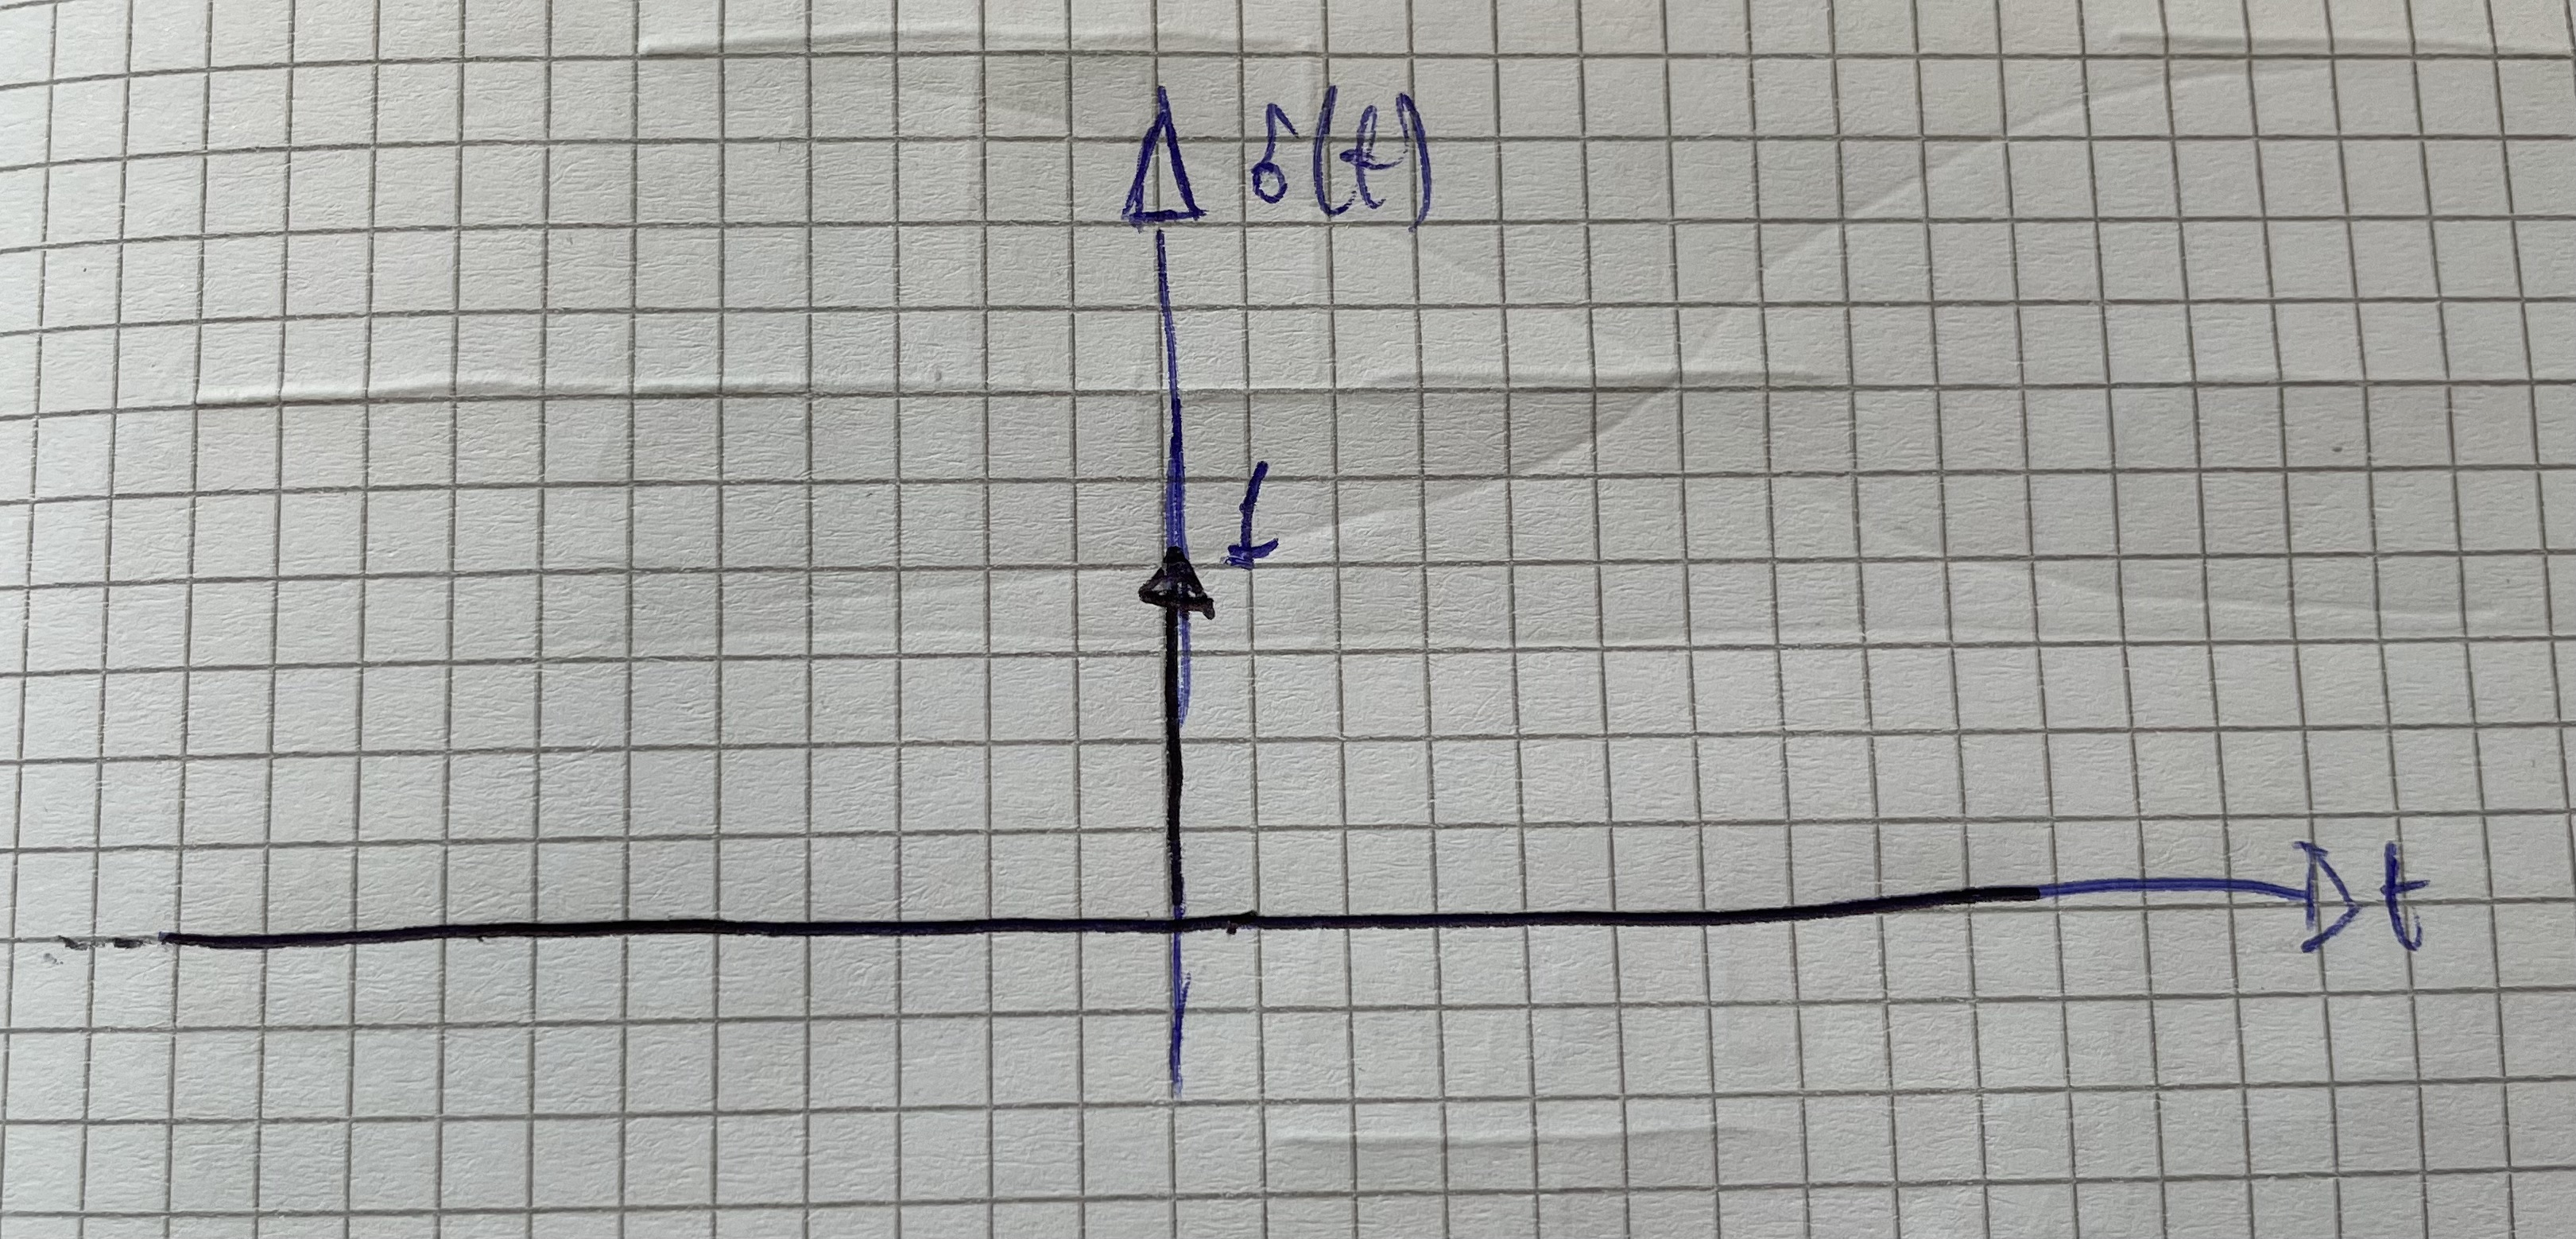
\includegraphics[scale=0.10]{images/12.Dirac.jpeg}
\end{figure} 
\subsubsection{\underline{Proprietà Campionatrice della Delta}}
$\int_{- \infty}^{+ \infty} f(x) \cdot \delta(x - x_0) dx = \int_{- \infty}^{+ \infty} f(x) \cdot \delta(x_0 - x) dx = f(x_0) \; \forall f(x) \text{ continua in } x_0$
\subsubsection{\underline{Proprietà}}
\begin{enumerate}
    \item $\delta(t)$ è una funzione pari: $\int_{- \infty}^{+ \infty} f(t) \cdot \delta(t) dt = \int_{- \infty}^{+ \infty} f(t) \cdot \delta(-t) dt = f(0)$
    \item Ha area unitaria: $f(t) = 1 \implies \int_{- \infty}^{+ \infty} \delta(t) dt = 1$
    \item $f(t) = \Pi\left( \frac{t}{\Delta}\right) \implies \int_{- \infty}^{+ \infty} \Pi\left( \frac{t}{\Delta}\right) \cdot \delta(t) dt = \int_{- \frac{\Delta}{2}}^{+ \frac{\Delta}{2}} \Pi\left( \frac{t}{\Delta}\right) \cdot \delta(t) dt = \int_{- \frac{\Delta}{2}}^{+ \frac{\Delta}{2}} \delta(t) dt = 1 \; \forall \Delta \in \mathbb{R}$
    \item $\int_{- \infty}^{x} \delta(z) dz = u(x) =  \begin{cases} 
    1 & \text{se } t > 0 \\
    0 & \text{se } t < 0 \\
    \end{cases}
    \implies 
    \delta(x) = \frac{d u(x)}{dx} \rightarrow \text{Derivata di una funzione discontinua}$
\end{enumerate}
\newpage
\subsubsection{\underline{Grafico}} ~\\
\begin{figure}[ht]
\centering
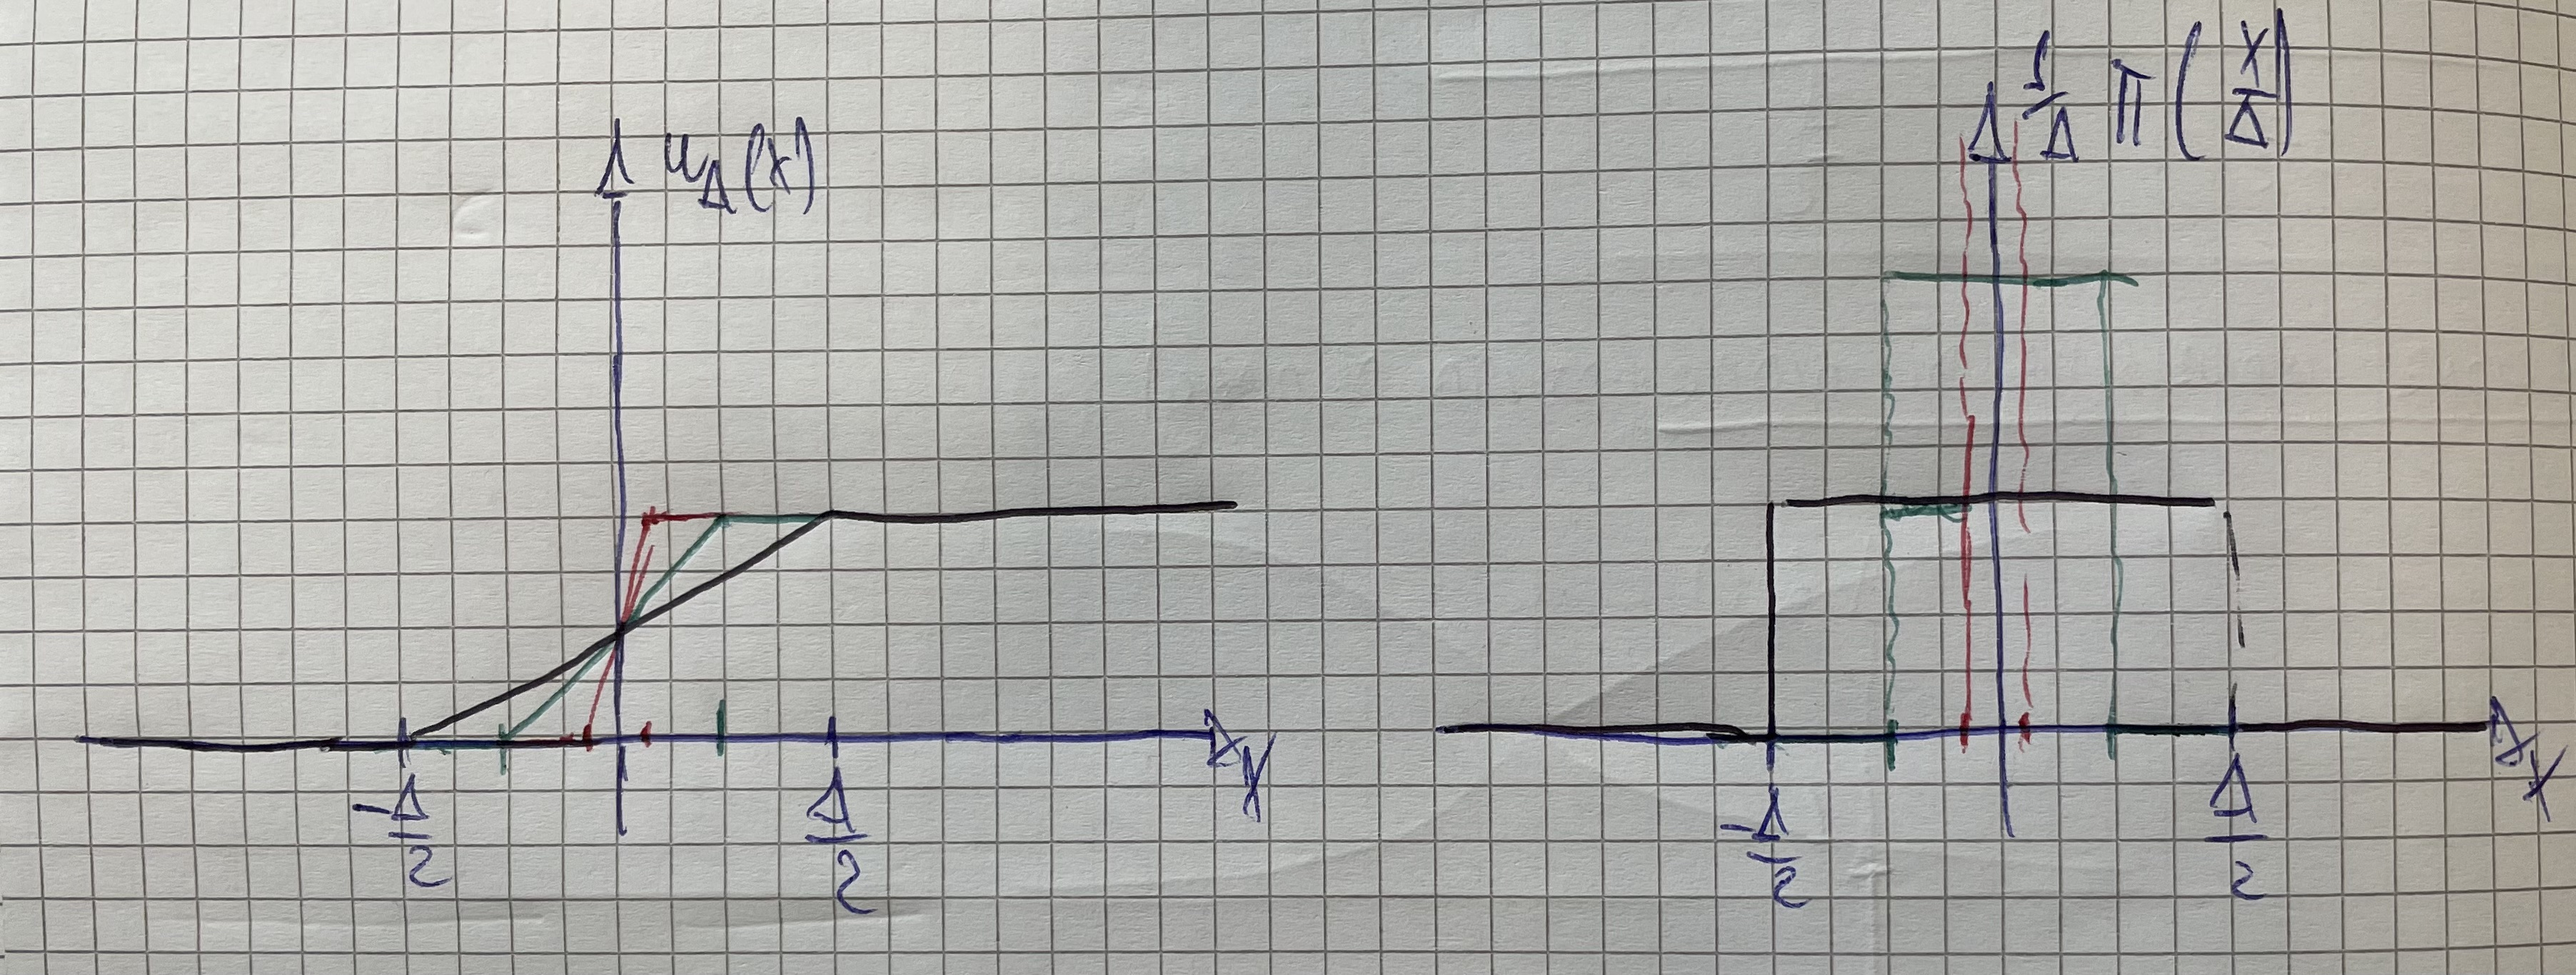
\includegraphics[scale=0.10]{images/13.Dirac2.jpeg}
\end{figure} 

\section{Fondamenti di Insiemistica}

\subsection{Insiemi}
Gli insiemi vengono indicati sempre con lettere maiuscole:
\subsubsection{\underline{Esempio}}
$A=\{ a_1,a_2, \dots , a_n\}, \;  a_2 \in A, \; b \notin A$ \\
$B = \{ x \in \mathbb{R} , 0 \leq x \leq 1\}$ \\
$C = \{ n \in \mathbb{N}\}$ \\

\subsection{Cardinalità o Dimensione}
Si dice cardinalità o dimensione di un insieme il numero degli elementi da cui esso è composto.
\subsubsection{\underline{Esempio}}
$Card(A) =n$ \\
$Card(B) = \text{Infinita non numerabile}$ \\
$Card(C) = \text{Infinita numerabile}$

\subsection{Sottoinsiemi}
Si dice che $B$ è un sottoinsieme di $A$ $\left( B \subset A\right)$ se tutti gli elementi di $A$ appartengono a $B$ e viceversa.
\subsubsection{\underline{Grafico}} ~\\
\begin{figure}[ht]
\centering
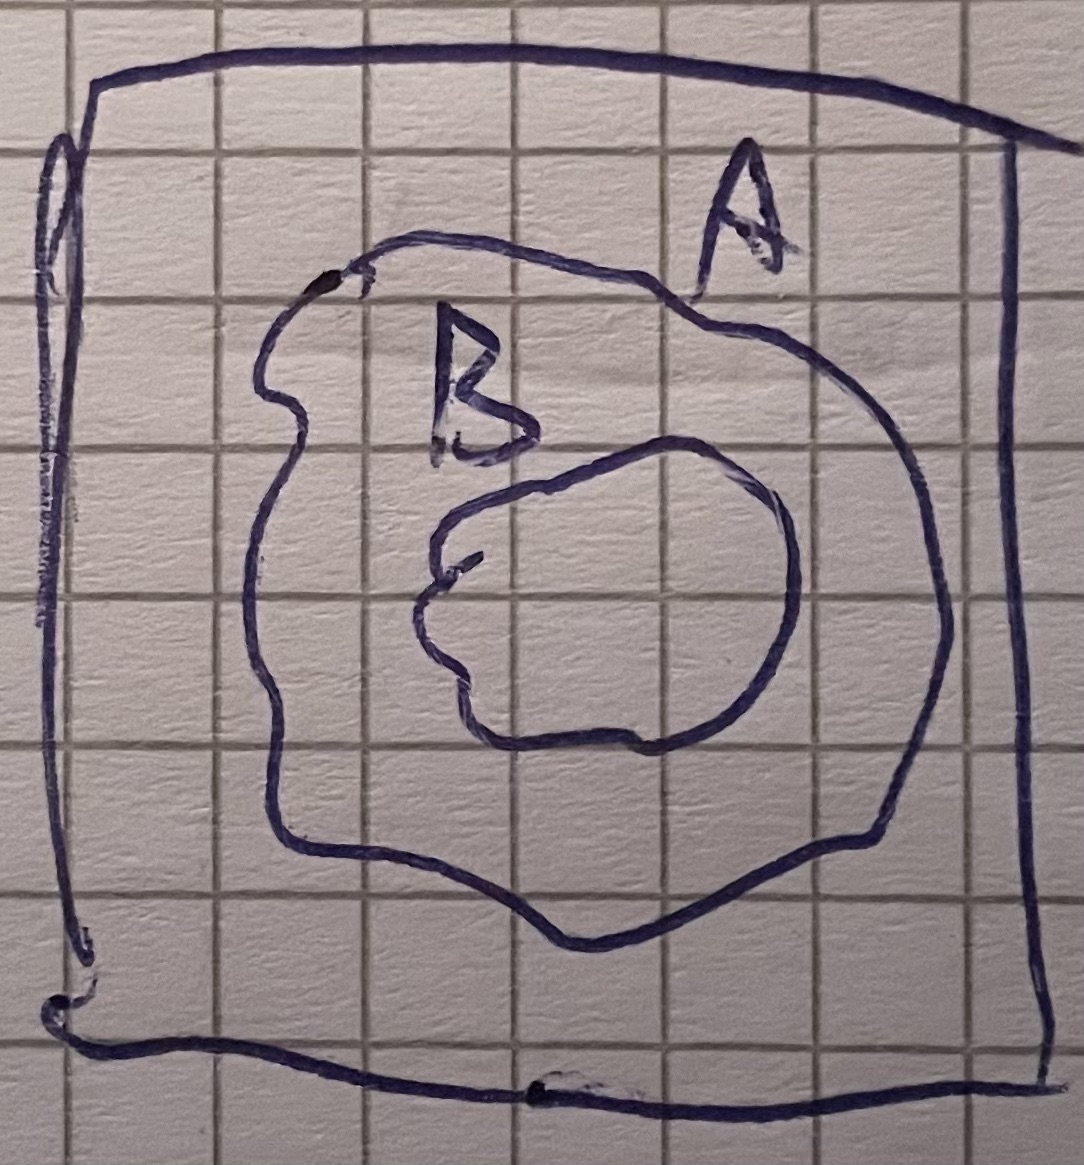
\includegraphics[scale=0.10]{images/14.VennSotto.jpeg}
\end{figure} 
\subsection{Insiemi Uguali}
Due insiemi si dicono uguali $\left( A = B \right)$ se tutti gli elementi di $A$ appartengono a $B$ e viceversa.

\subsection{Spazio Campione e Insieme Vuoto}
Da qui in avanti supporremo che tutti gli insiemi che vedremo saranno sottoinsiemi di $\Omega \text{ (Omega)}$, detto anche Insieme Universale o \textbf{Spazio Campione}. \\ \\
\textbf{L'insieme vuoto} $\phi \text{(Phi)}$ non è composto da alcun elemento $\left( Card(\phi) = 0\right)$ e per convenzione è sottoinsieme di qualsiasi insieme. \\ \\
Come ad esempio: $\phi \subset A$

\subsection{Diagrammi di Venn}
Per rappresentare gli insiemi si utilizzano i diagrammi di Venn, che sono fatti in questo modo:
\subsubsection{\underline{Grafico}} ~\\
\begin{figure}[ht]
\centering
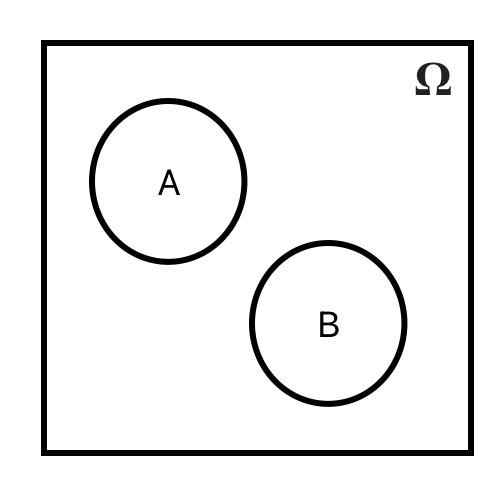
\includegraphics[scale=0.40]{images/15.Venn.png}
\end{figure} 

\subsection{Unione (o Somma)}
$C = A +B = A \cup B$ \\
L’insieme $C$ contiene ogni elemento che appartiene o ad $A$ o a $B$. \\
Detto in altri termini: contiene tutti gli elementi di $A$ e tutti gli elementi di $B$.
\subsubsection{\underline{Grafico}} ~\\
\begin{figure}[ht]
\centering
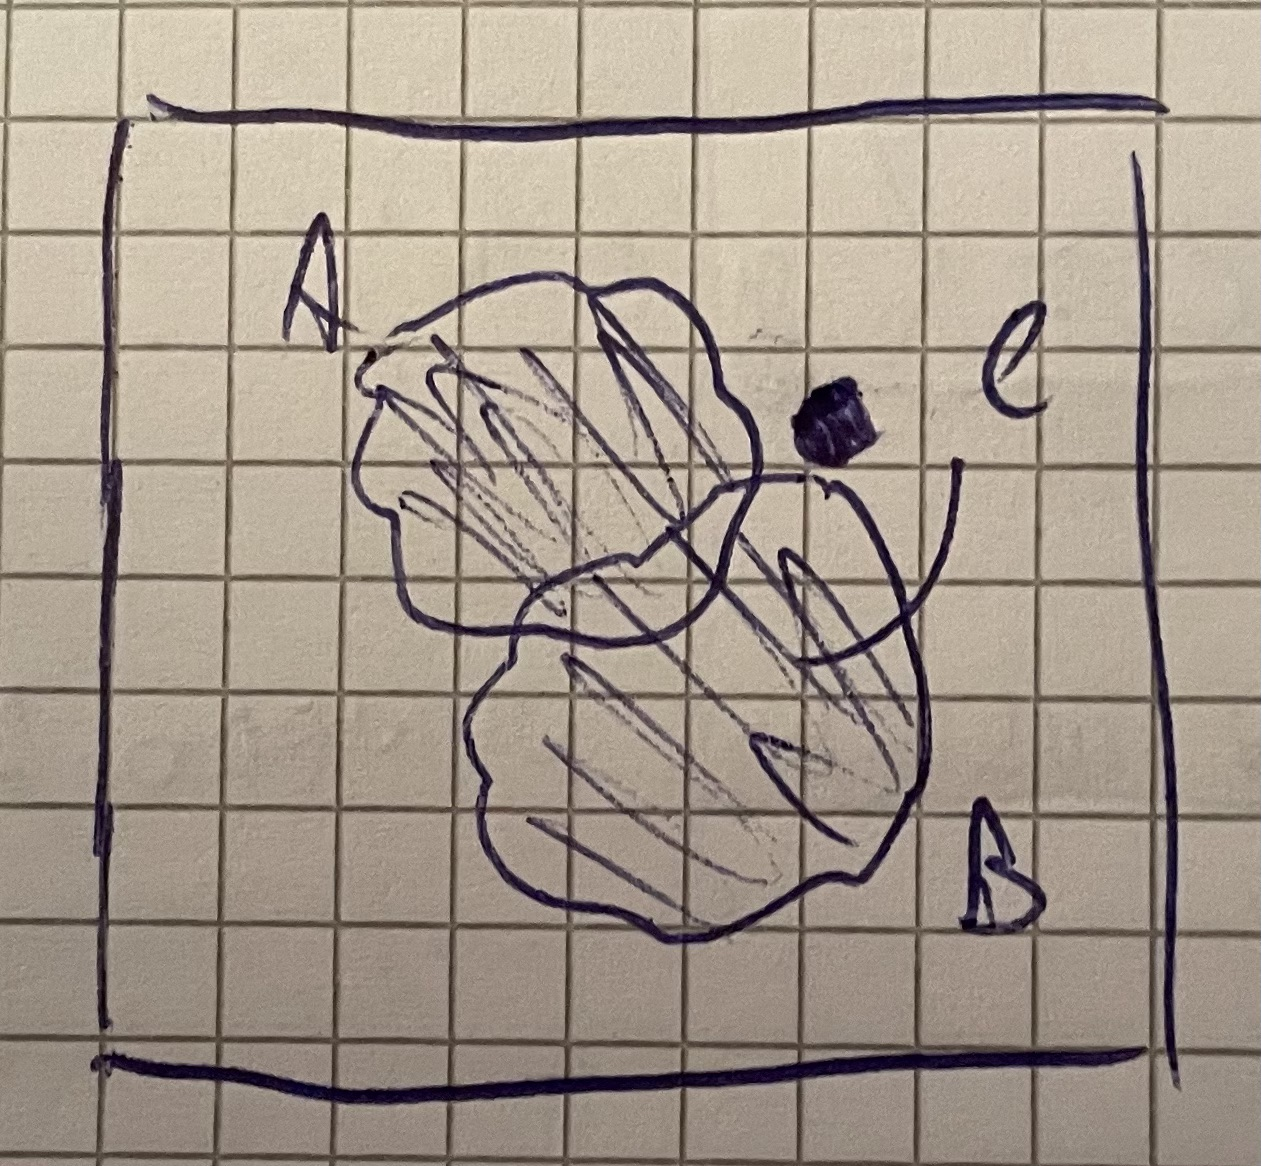
\includegraphics[scale=0.13]{images/16.VennSomma.jpeg}
\end{figure} 
\subsubsection{\underline{Proprietà}}
\begin{itemize}
    \item Proprietà commutativa $A + B = B + A$
    \item Proprietà associativa $A + B + C = (A + B) + C = A + (B + C)$
    \item Se $B \subset A$ allora $A + B = A$
    \item $A + \phi = A$
    \item $A + A = A$
    \item $A + \Omega = \Omega$
\end{itemize}

\subsection{Intersezione (o Prodotto)}
$C = A \cdot B = A \cap B$ \\
L’insieme $C$ contiene tutti gli elementi in comune fra $A$ e $B$.
\subsubsection{\underline{Grafico}} ~\\
\begin{figure}[ht]
\centering
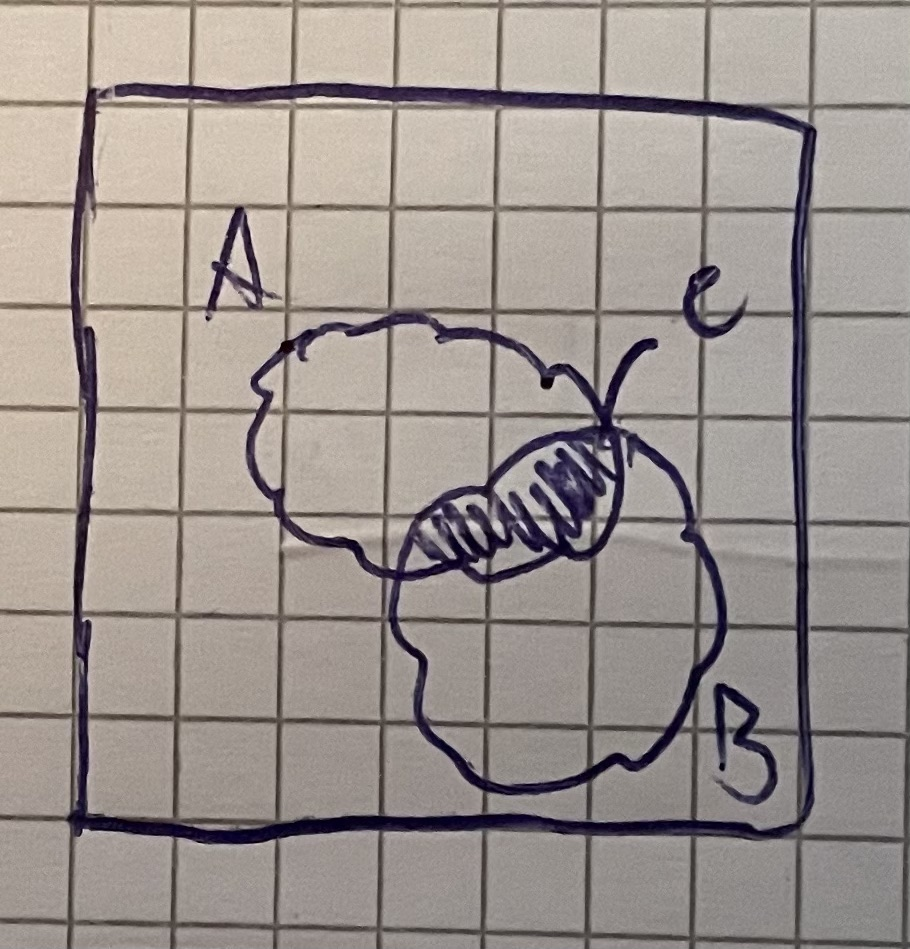
\includegraphics[scale=0.13]{images/17.VennProdott.jpeg}
\end{figure} 
\subsubsection{\underline{Proprietà}}
\begin{itemize}
    \item Proprietà commutativa $A \cdot B = B \cdot A$
    \item Proprietà associativa $A \cdot B \cdot C = (A \cdot B) \cdot C = A \cdot (B \cdot C)$
    \item Se $B \subset A$ allora $A \cdot B = B$
    \item $A \cdot \phi = \phi$
    \item $A \cdot A = A$
    \item $A \cdot \Omega = A$
\end{itemize}
\subsubsection{\underline{Esempio}}
Spazio Campione: $\Omega=\{ 1,2,3,4,5,6\} $ \\
$A = \{ \text{Numeri Pari} \} = \{ 2,4,6\}$ \\
$A = \{ \text{Numeri Maggiori di } 3 \} = \{ 4,5,6 \}$ \\ \\
$A + B = \{ 2,4,5,6\} \;\; | \;\; A \cdot B = \{ 4,6 \} = \{ \text{Numeri pari e maggiori di } 3\}$

\subsection{Insiemi Disgiunti}
$A$ e $B$ si dicono disgiunti se $A \cdot B = \phi$
\subsubsection{\underline{Esempio}}
$A_1,A_2, \dots , A_n $ sono tutti disgiunti se e solo se sono disgiunti a due a due, ovvero: $A_i \cdot A_j = \phi$

\subsection{Partizioni di A}
Siano $B_1,B_2, \dots, B_n$ disgiunti tali che: $\begin{matrix}
B_1 + B_2 + \dots + B_n = A \\
\Updownarrow \\
\bigcup\limits_{i=1}^{n} B_i = \sum\limits_{i=1}^{n} B_i= A
\end{matrix}$
\subsubsection{\underline{Grafico}} ~\\
\begin{figure}[ht]
\centering
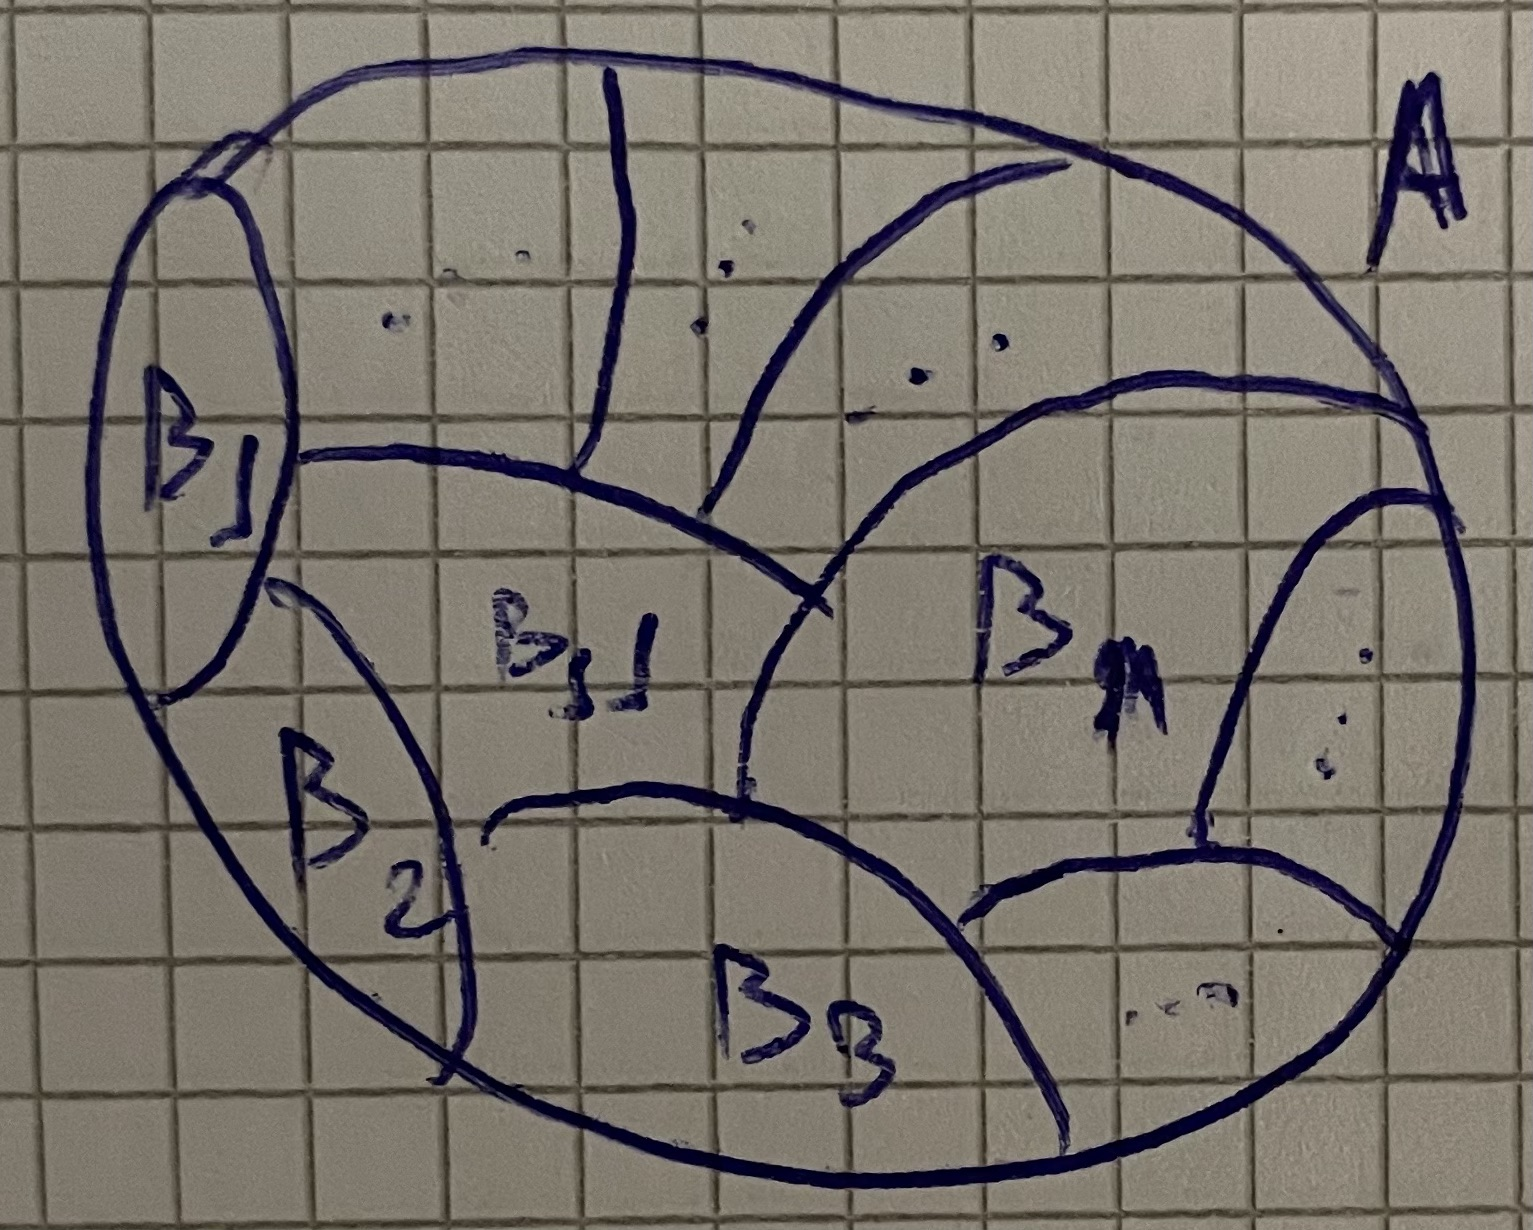
\includegraphics[scale=0.13]{images/18.Partizione.jpeg}
\end{figure} 

\subsection{Complementare di un insieme}
Il complementare dell'insieme $A$, ovvero $\overline{A}$ è costituito da tutti gli elementi di $\Omega$ che non appartengono ad $A$.
\subsubsection{\underline{Grafico}} ~\\
\begin{figure}[ht]
\centering
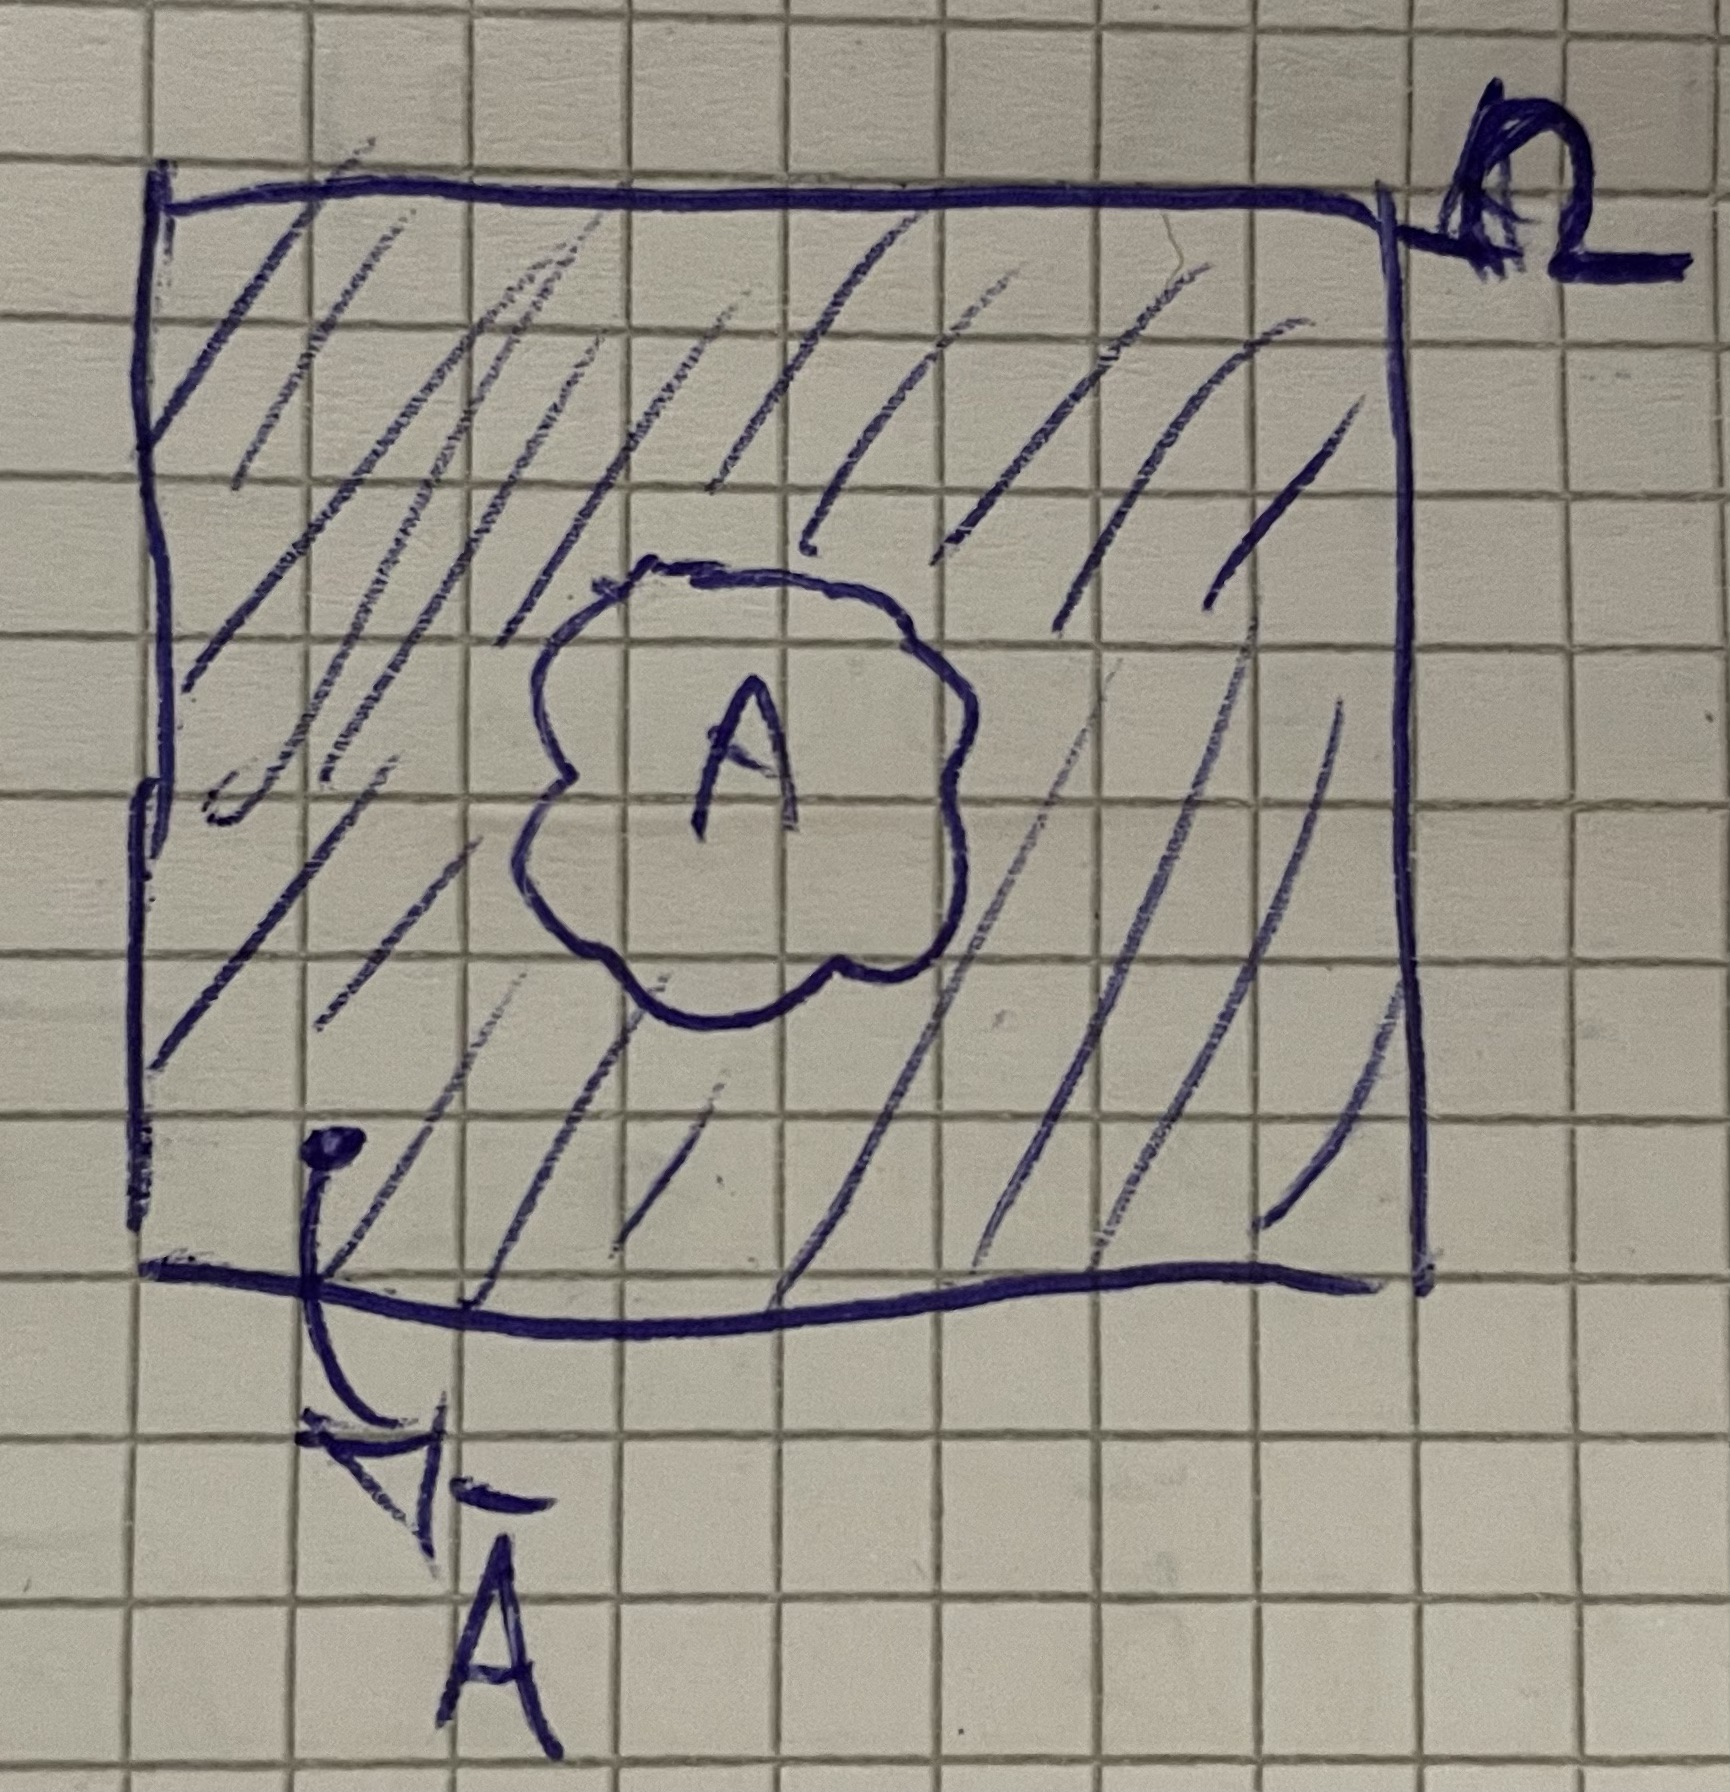
\includegraphics[scale=0.13]{images/19.VennCompl.jpeg}
\end{figure} 
\subsubsection{\underline{Proprietà}}
\begin{itemize}
    \item $\overline{\overline{A}} = A$
    \item $A \cdot \overline{A} = \phi$
    \item $A + \overline{A} = \Omega$
    \item $\overline{\phi} = \Omega$
    \item $\overline{\Omega} = \phi$
\end{itemize}

\subsection{L’Insieme Differenza}
$C = A-B = A \backslash B$ \\
L’insieme $C$ è composto dagli elementi di $A$ che non appartengono a $B$. \\
Detto in altre parole, l’insieme $C$ è composto dagli elementi di $A$ meno gli elementi di $B$. \\
È importante sapere che $a \in A-B \iff a \in A, a \in B$
\subsubsection{\underline{Grafico}} ~\\
\begin{figure}[ht]
\centering
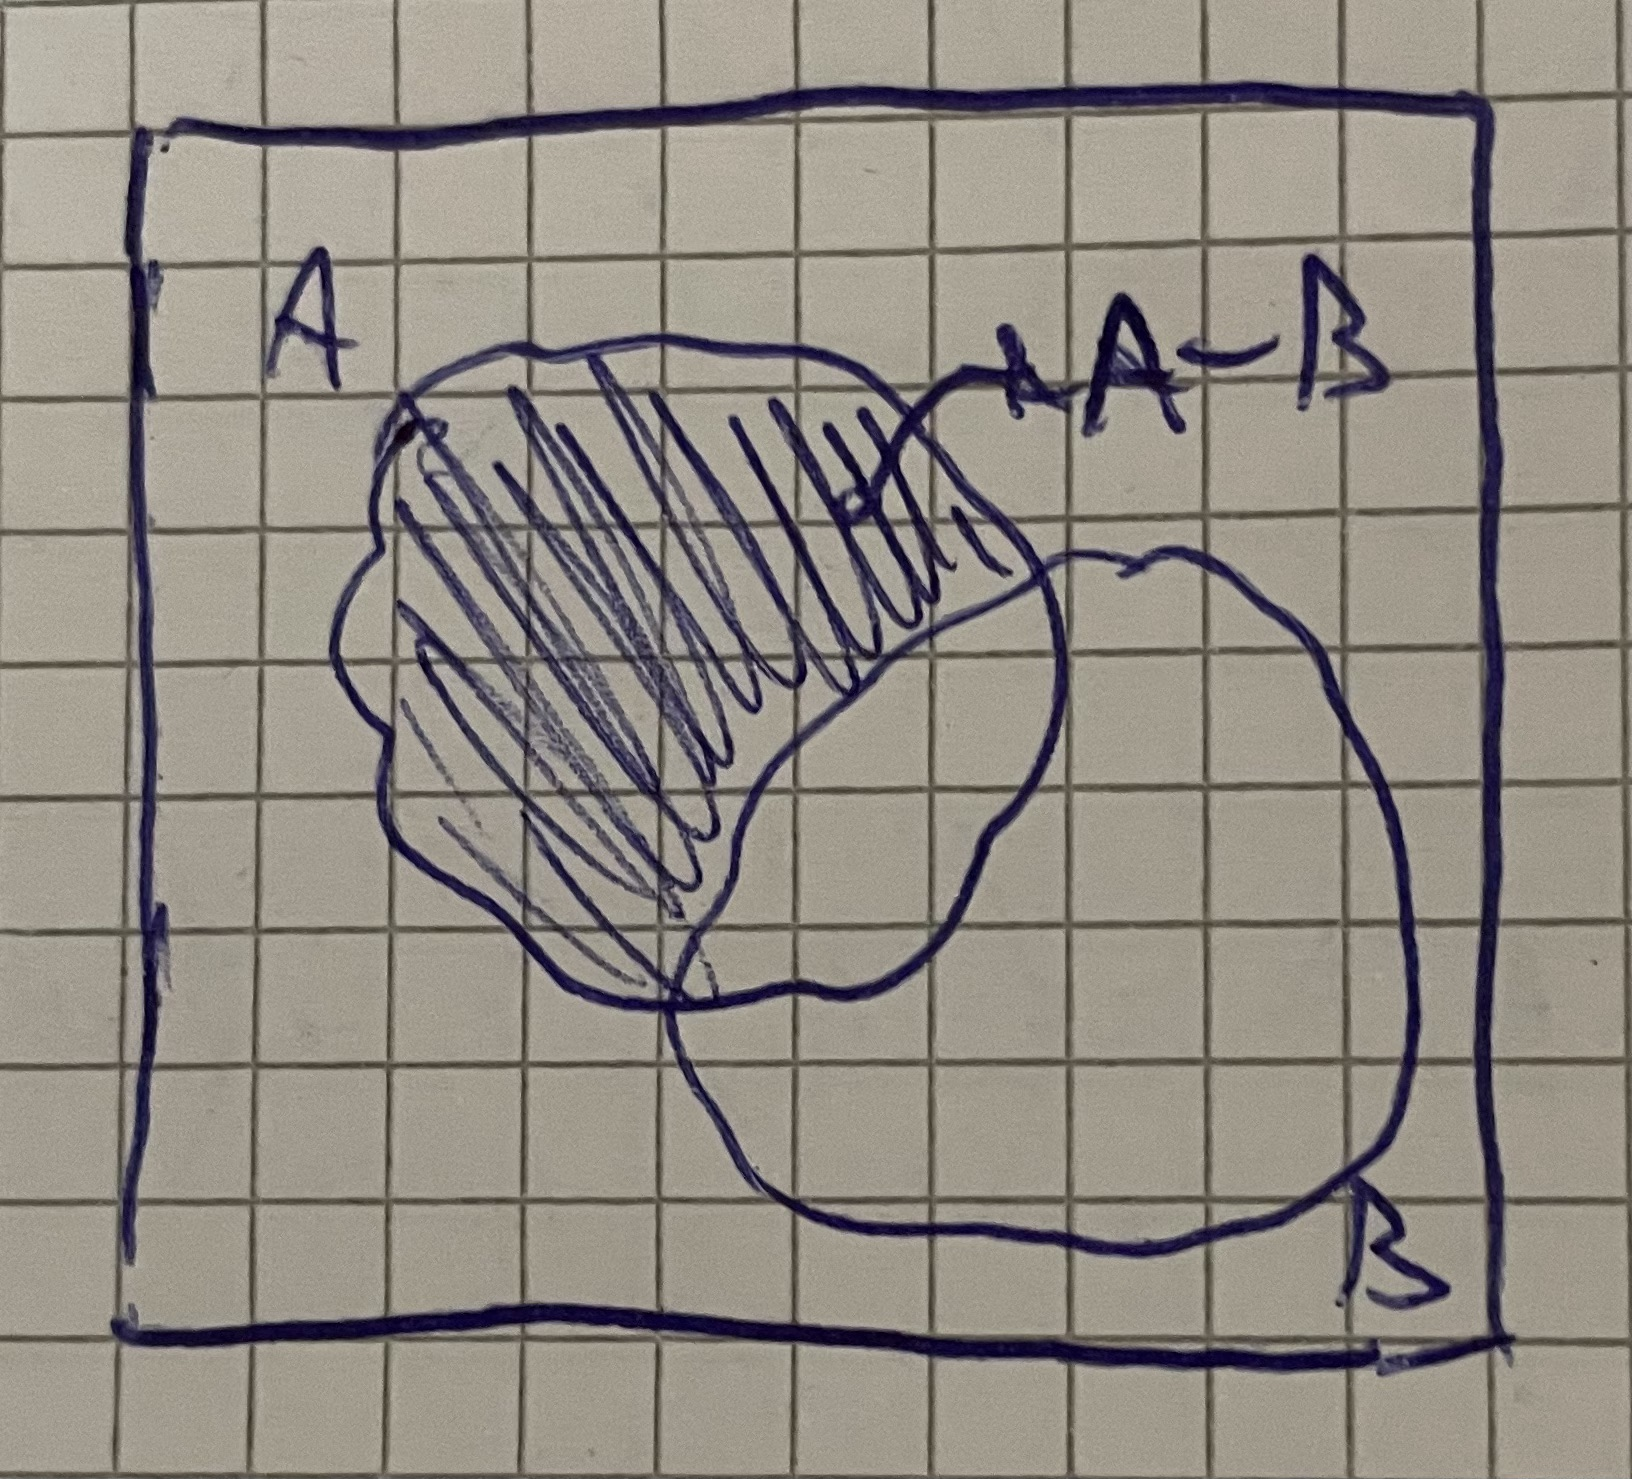
\includegraphics[scale=0.13]{images/20.VennDiff.jpeg}
\end{figure} 
\subsubsection{\underline{Proprietà}}
\begin{itemize}
    \item $A-B=A-AB = A \cdot \overline{B}$
    \item Non vale la proprietà commutativa.
    \item Non vale la proprietà associativa.
    \item $\left( A - A \right) + A = A \; \begin{bmatrix} (A-A)+A = \phi +A = A \end{bmatrix}$
    \item $\left( A + A \right) - A = \phi \; \begin{bmatrix} (A+A)-A = A - A = \phi \end{bmatrix}$
    \item $(A - B) +B = A+B$
    \item $A - (B-B) = A - \phi = A$
    \item $A- \phi = A$
    \item $\Omega - A = \overline{A}$
    \item $A - \Omega = \phi$
\end{itemize}
\subsubsection{\underline{Esempio}}
$\Omega = \{ 1,2,3,4,5,6 \} \; \big| \; A=\{ 1,2,3 \} \; \big| \; B =\{ 2,3,4\}$ \\
$A + B = \{ 1,2,3,4 \} \; \big| \; A \cdot B = \{ 2,3 \}$ \\
$A - B = \{ 1 \}$ \\
$\overline{A} = \{ 4,5,6 \} \; \big| \; \overline{B} = \{ 1,5,6 \}$

\subsection{Uguaglianze(Leggi) di DeMorgan}
\begin{enumerate}
    \item $\overline{A \cup B} = \overline{A} \cap \overline{B} \iff \overline{A + B} = \overline{A} \cdot \overline{B}$
    \item $\overline{A \cap B} = \overline{A} \cup \overline{B} \iff \overline{A \cdot B} = \overline{A} + \overline{B}$
\end{enumerate}

\subsection{Proprietà Distributiva Dell’Intersezione Rispetto All’Unione}
$\begin{matrix}
A \cdot (B + C) = A \cdot B + A \cdot C \\
\parallel \\
A \cap (B \cup C) = A \cap B \cup A \cap C
\end{matrix}$
\subsection{Trasformare le Operazioni fra Insiemi}
\begin{tabular}{|p{13cm}}
In un’uguaglianza tra insiemi, se trasformo ogni unione in un’intersezione, ogni intersezione con un’unione e ogni insieme con il suo complementare, l’uguaglianza non cambia.
\end{tabular} \\ \\
Possiamo schematizzare queste trasformazioni in due gruppi: \\
$\begin{matrix}
1) & \cup \rightarrow \cap && 2) & \cup \rightarrow \cap \\
& \cap \rightarrow \cup && & \cap \rightarrow \cup \\
& A \rightarrow \overline{A} && & \phi \rightarrow \Omega \\
&  && & \Omega \rightarrow \phi \\
\end{matrix}$ \\
\begin{tabular}{|p{13cm}}
Per far valere le uguaglianze, senza cambiare il risultato, possiamo utilizzare il primo gruppo di trasformazioni o il secondo, ma \textbf{NON} tutti e due insieme.
\end{tabular}
\subsubsection{\underline{Dimostrazione}}
$\begin{matrix}
\overline{A \cdot (B+C)} = \overline{A \cdot B + A \cdot C} & \\
\downarrow & \text{Applico DeMorgan} \\
\overline{A} + \overline{(B+C)} = \overline{A \cdot B} \cdot \overline{A \cdot C} & \\
\downarrow & \text{Applico di nuovo DeMorgan} \\
\overline{A} + \overline{B} \cdot \overline{C} = \left(\overline{A} + \overline{B} \right) \cdot \left( \overline{A} + \overline{C} \right)
\end{matrix}$ \\
\hspace*{0pt}\hfill $\square$ 
\subsubsection{\underline{Esempio}}
$\begin{matrix}
A \cap (B \cup C) = (A \cap B) \cup (A \cap C) & \equiv & A \cdot (B + C) = (A \cdot B) + (A \cdot C) \\
& \parallel & \\
\overline{A} \cup \overline{B} \cap \overline{C} = \left( \overline{A} \cup \overline{B} \right) \cap \left( \overline{A} \cup \overline{C} \right) & \equiv & 
\overline{A} + \overline{B} \cdot \overline{C} = \left( \overline{A} + \overline{B} \right) \cdot \left( \overline{A} + \overline{C} \right)
\end{matrix}$

\subsection{Determinare il Numero Massimo di Sotto-Insiemi di un Insieme}
$A = \{ a_1,a_2, \dots , a_n \}$ \\
Il numero massimo di sottoinsiemi che può avere l’insieme $A$ dato dal numero di \textbf{disposizioni con ripetizioni} di $A$, ovvero $\color{red} 2^n$. \\ \\
Per comprendere meglio quanti sottoinsiemi può avere l’insieme $A$ possiamo utilizzare le \textbf{$n$-uple di bit}, ovvero, in ogni suo sottoinsieme se un certo elemento di $A$ è presente al suo interno, lo indichiamo con un $1$, se invece non è presente lo indichiamo con uno $0$. \\
\[\begin{matrix}
\{ \phi \} = \{0, 0, 0, \dots , 0\} \\
\{ a_1 \} = \{1, 0, 0, \dots , 0\} \\
\{ a_2 \} = \{0, 1, 0, \dots , 0\} \\
\vdots \\
\{a_1 , a_3 \} = \{ 1, 0, 1, 0, \dots , 0\} \\
\vdots \\
\{a_1, a_2, \dots , a_n\} = \{1, 1, \dots, 1\}
\end{matrix}\] \\
Possiamo indicare il numero massimo di sottoinsiemi come: $\sum_{k = 0}^{n} \left( \begin{matrix} n \\ k\end{matrix} \right)$. \\
Se tutte e due le risposte sono giuste, allora: $2^n =\sum_{k = 0}^{n} \left( \begin{matrix} n \\ k\end{matrix} \right)$. \\
Come possiamo notare questa uguaglianza non è altro che un caso particolare del Binomio di Newton: \\ $(a+b)^n = \sum_{k = 0}^{n} \left( \begin{matrix} n \\ k\end{matrix} \right) a^kb^{n-k}$

\section{Introduzione alla Probabilità}

\subsection{Eventi ed Esperiment}
\begin{itemize}
    \item Definiamo \textbf{Esperimento Casuale} un’operazione la quale soluzione non è predicibile (es. lancio di dadi, lancio moneta, ecc…).
    \item Definiamo come \textbf{Evento} un insieme di risultati con una probabilità comune.
    \item Un \textbf{Evento Elementare} è un evento caratterizzato da un solo risultato (es. una faccia di un dado) ed è un sottoinsieme dell’evento.
    \item Dato l’evento $A$, allora anche $\overline A$ è a sua volta un evento.
    \item L’unione di più eventi è a sua volta un evento.
    \item L’intersezione di più eventi è a sua volta un evento.
    \item Lo spazio campione $\Omega$ è un evento detto \textbf{Evento Certo}.
    \item L’insieme nullo $\phi$ è un evento detto \textbf{Evento Nullo} o \textbf{Evento Impossibile}.
    \item Gli eventi rappresentano un \textbf{Campo} (o un \textbf{Algebra}).
    \item Se gli eventi sono numerabili si chiama \textbf{Campo di Borel}.
    \item Gli elementi dell’evento $A$ si chiamano \textbf{Risultati Favorevoli}.
    \item Se $A \cdot B = \phi$, ovvero gli insiemi sono disgiunti, allora si dice che gli eventi sono \textbf{incompatibili} o detto in un altro modo, gli eventi sono \textbf{mutuamente esclusivi}.
    \item $a \in \Omega$ si dice \textbf{Evento Elementare}
    \item $Card\{ \Omega \} = \begin{cases} 
        \text{Finita}  \implies \bf{Spazio} \; Campione \; Discreto\\
        \text{Infinita Numerabile} \implies \bf{Spazio} \; Campione \; Discreto\\
        \text{Inifnita Non Numerabile} \implies \bf{Spazio} \; Campione \; Continuo
        \end{cases}$
    \item $\mathcal{I} \left( \text{"i" corsiva maiuscola} \right)$ indica una \textbf{Classe/Famiglia degli Eventi}, ovvero definisce un \textbf{Campo/Algebra}.
\end{itemize}

\subsection{Teoria Assiomatica della Probabilità(Kolmogorov 1933)}
La probabilità di un evento $P(A)$ è una qualunque funzione che va da $\mathcal{I}$ a $\mathbb{R}$ $\left( \mathcal{I} \rightarrow \mathbb{R} \right)$ e che gode di \textbf{3 fondamentali assiomi}:
\begin{enumerate}
    \item $P\left(\Omega\right) = 1$
    \item $P(A) \geq 0 \;\;\forall A$
    \item $P(A_1 +A_2) = P(A_1) + P(A_2) \; \; se \;\; A_1 \cdot A_2 = \phi \left(\text{Sono disgiunti}\right)$
\end{enumerate} 
La probabilità è detta misura normalizzata, poiché la probabilità massima arriva al massimo ad 1.
\subsubsection{\underline{Esempio}}
Nell’esempio prenderemo in indagine il lancio di una moneta, ma supporremo che la probabilità che esca testa o croce sia diversa da $0.5$ e $0.5$, cosa ovviamente impossibile. \\ \\
$\Omega \{Testa,Croce\} \;\big|\; P(T) = 0,9 > 0 \:\big|\; P(C) = 0,1>0$ \\
$T \cap C = \phi $ \\
$P(\Omega) = P(T) + P(C) = 0,9 +0,1 = 1$

\subsection{Frequenza di Presentazione}
Definiamo Frequenza di Presentazione (o Frequenza Relativa) come:
\[f(A) = \frac{n_A}{n}\]

\subsection{Definizione di Probabilità}
Definiamo la probabilità come:
\[P(A) = \lim_{n \to +\infty} f(A) = \lim_{n \to +\infty} \frac{n_A}{n}\]
Possiamo facilmente vedere che verifica i 3 assiomi:
\begin{enumerate}
    \item $n_\Omega = n \implies f(\Omega) = 1$
    \item $f(A) \geq 0$
    \item $n_{A+B} = n_A + n_B$
\end{enumerate}
Dal terzo assioma possiamo dedurre che: \\
$f(A_1 + A_2) = \frac{n_{A_1 + A_2}}{n} = \frac{n_{A_1} +n_{A_2}}{n} = \frac{n_{A_1}}{n} + \frac{n_{A_2}}{n} = f(A_1) + f(A_2)$

\subsection{Proprietà dei 3 Assiomi}
Dai 3 assiomi possiamo dedurre alcune proprietà:
\begin{itemize}
    \item Dal terzo assioma possiamo dedurre che se $A_1, A_2 , \dots, A_n$ sono eventi disgiunti ed incompatibili $\left(A_i \cdot A_j = \phi\right)$ allora $\left(\implies \right)$ 
    \[\begin{matrix}
    P(A_1 + A_2 + \dots + A_n) \\
    = P(A_1) + P(A_2 + A_3 + \dots + A_n) \\
    = P(A_1) + P(A_2) + P(A_3 + \dots + A_n) \\
    = P(A_1) + P(A_2) + \dots + P(A_n) \\
    = \color{red} P\left( \sum\limits_{i = 1}^{n} A_i\right) = \sum\limits_{i = 1}^{n} P(A_i)
    \end{matrix}\]
    \item $P(\phi) = 0$ \\ 
    \subsubsection{\underline{Dimostrazione}} 
    Noi sappiamo che $\Omega = A + \overline{A} \text{ e } A \cdot \overline{A} = \phi$ \\
    Quindi possiamo dedurre che $P(\Omega) = 1 \implies P(A + \overline A) = 1 \implies P(A) + P(\overline A) = 1$ \\
    Dall'ultima possiamo capire che $P(A) + P(\overline A) = 1 \implies \color{red} P\left( \overline{A}\right) = 1 -P(A)$ \\ 
    \hspace*{0pt}\hfill $\square$ 
    \item \textbf{Monotonicità:} Se $B \subset A \implies P(A) \geq P(B)$ \\
    \subsubsection{\underline{Dimostrazione}} 
    Sappiamo che $A = B + \overline B \cdot A$ 
    \newpage
    \subsubsection{\underline{Grafico}} ~\\
    \begin{figure}[ht]
    \centering
    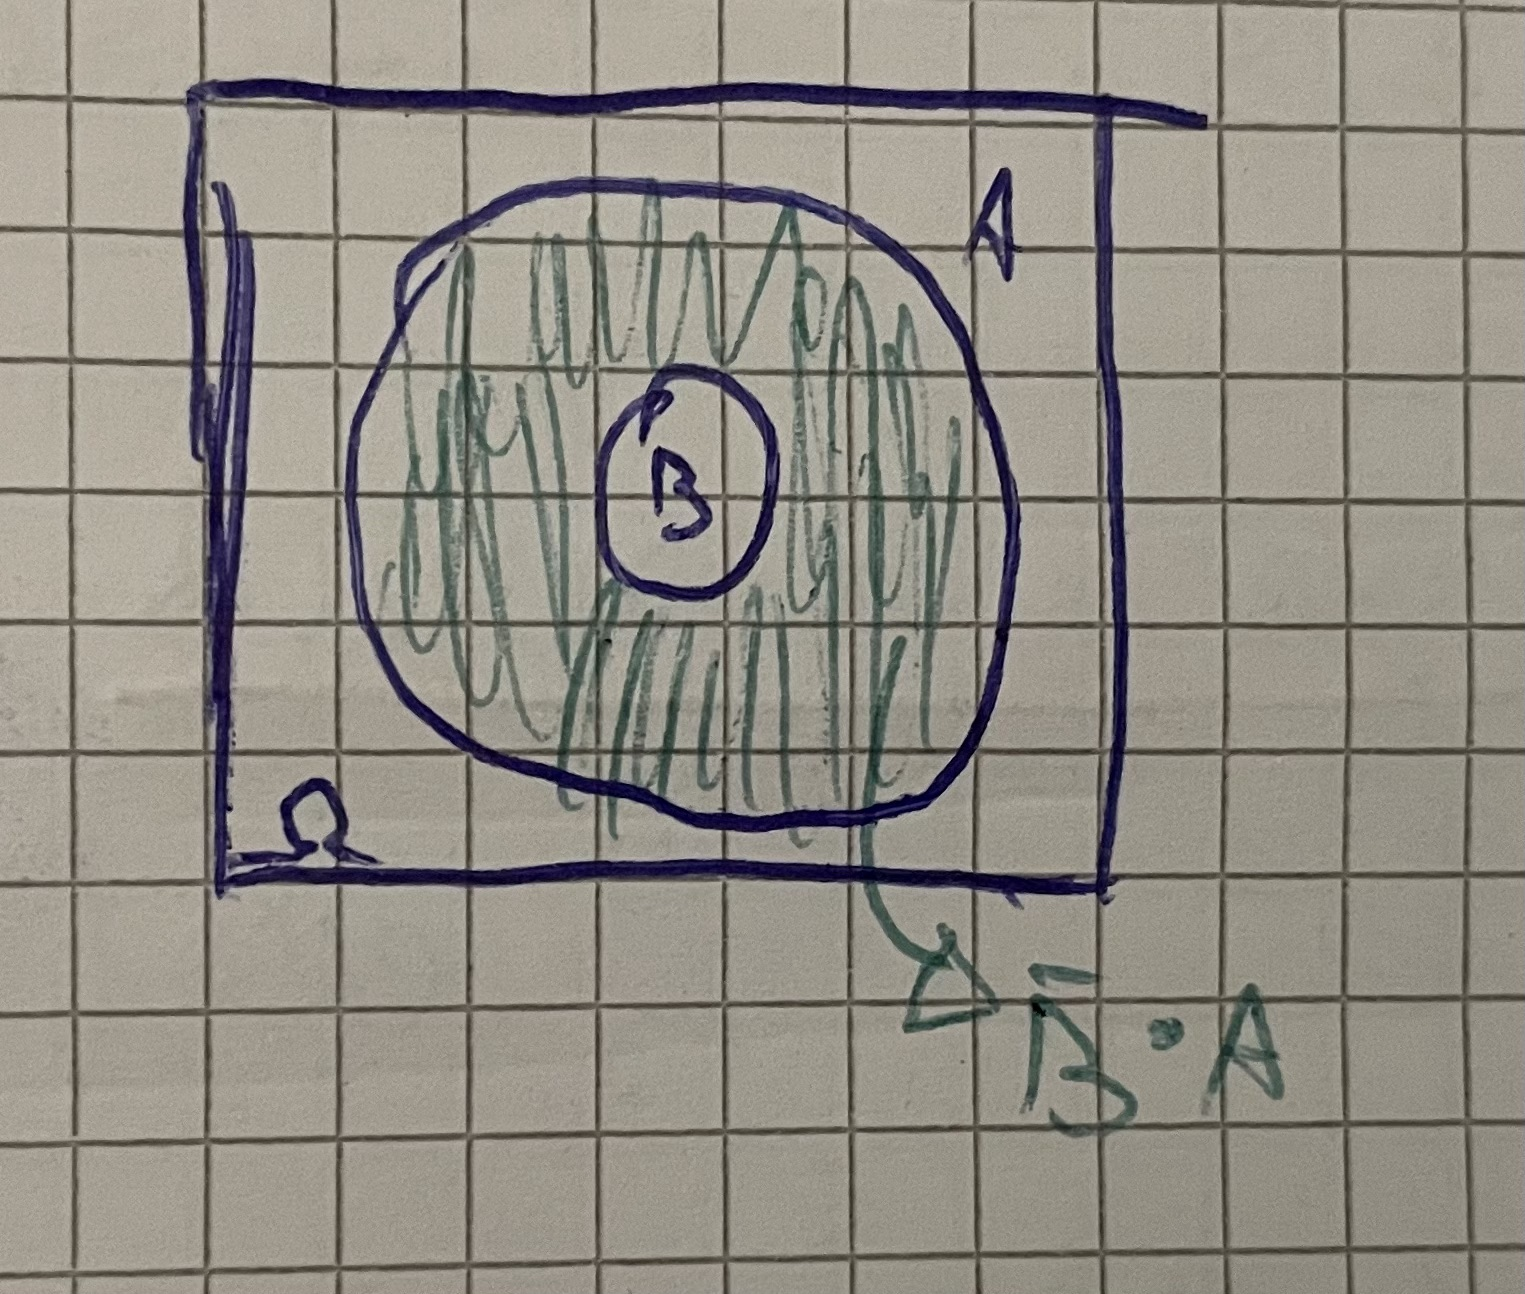
\includegraphics[scale=0.13]{images/21.Prop4_4.5.jpeg}
    \end{figure} \\
    Quindi $P(A) = P(B + \overline B\cdot A) = P(B) + P(\overline B \cdot A)$ \\
    Dal secondo assioma noi sappiamo che $P(\overline B \cdot A) \geq 0$, di conseguenza $P(A) \geq B$ \\
    \hspace*{0pt}\hfill $\square$ 
    \item Se $A \cdot B = \phi$ (Sono disgiunti) $\implies P(A+B) = P(A) + P(B) -P(A \cdot B)$
    \subsubsection{\underline{Dimostrazione}}
    \subsubsection{\underline{Grafico}} ~\\
    \begin{figure}[ht]
    \centering
    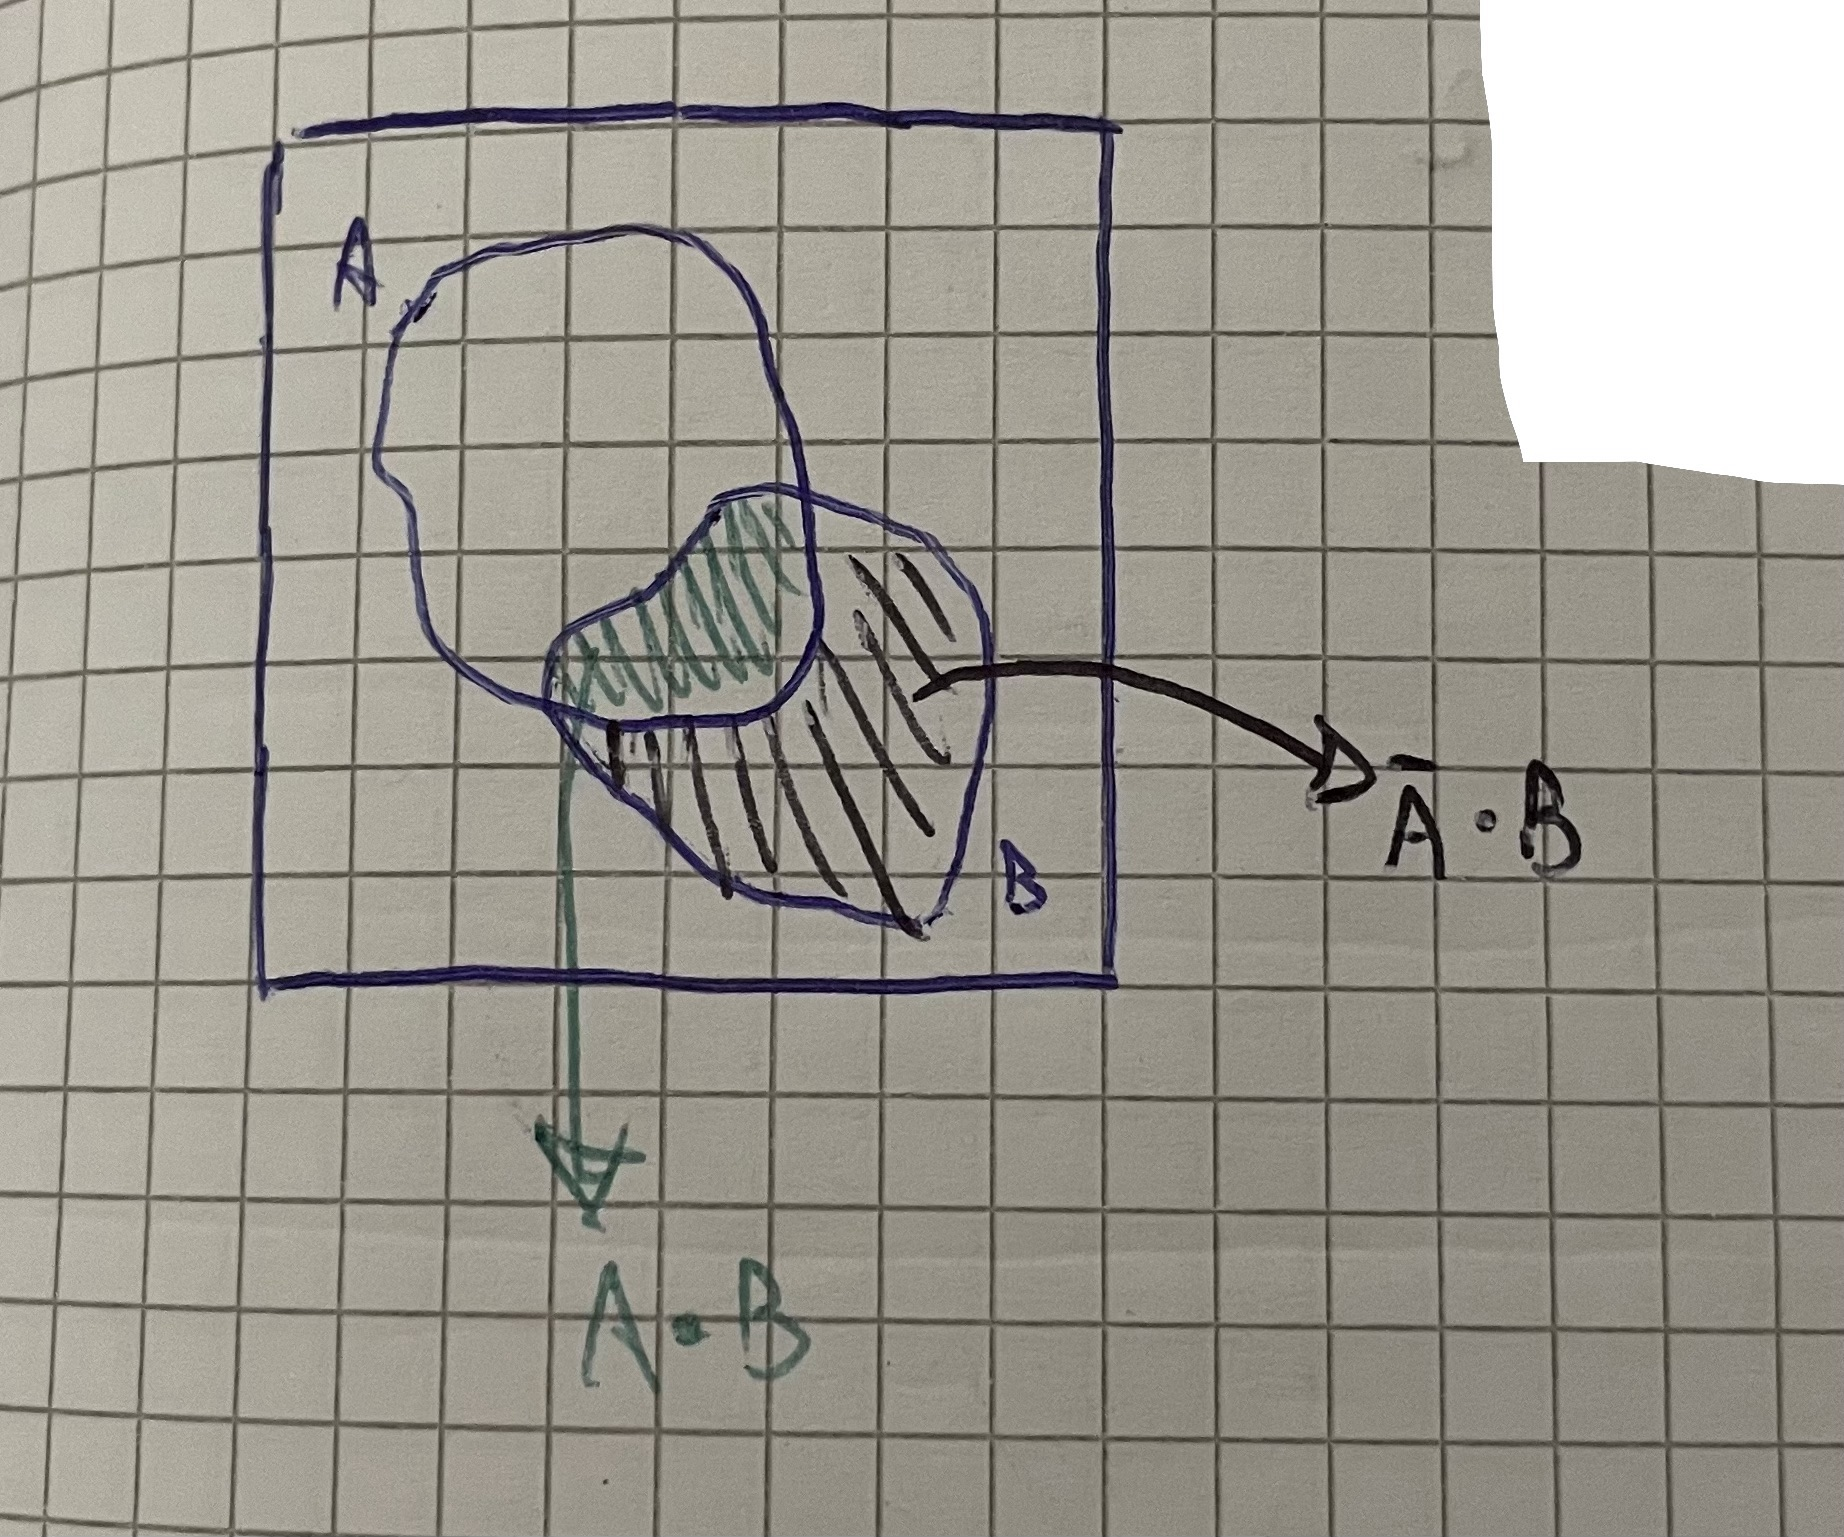
\includegraphics[scale=0.13]{images/22.Prop5_4.5.jpeg} 
    \end{figure} \\
    $\# A+B = A + \overline A \cdot B \implies P(A)+P(B) = P(A) + P(\overline A \cdot B)$ \\
    $\# B = (A \cdot B) + (\overline A \cdot B) \implies P(B) = P(A \cdot B) + P(\overline A \cdot B)$ \\
    $\Downarrow$ \\
    $P(A+B)-P(B) = P(A) + \cancel{P(\overline A \cdot B)} - P(A \cdot B) - \cancel{P(\overline A \cdot B)}$ \\
    $\implies P(A+B)-P(B) = P(A) - P(A \cdot B)$ \\
    $\implies \color{red}P(A+B) = P(A) + P(B) - P(A \cdot B)$ \\
    \hspace*{0pt}\hfill $\square$ 
\end{itemize}
\newpage
\subsubsection{\underline{Esempio}} 
\begin{figure}[ht]
\centering
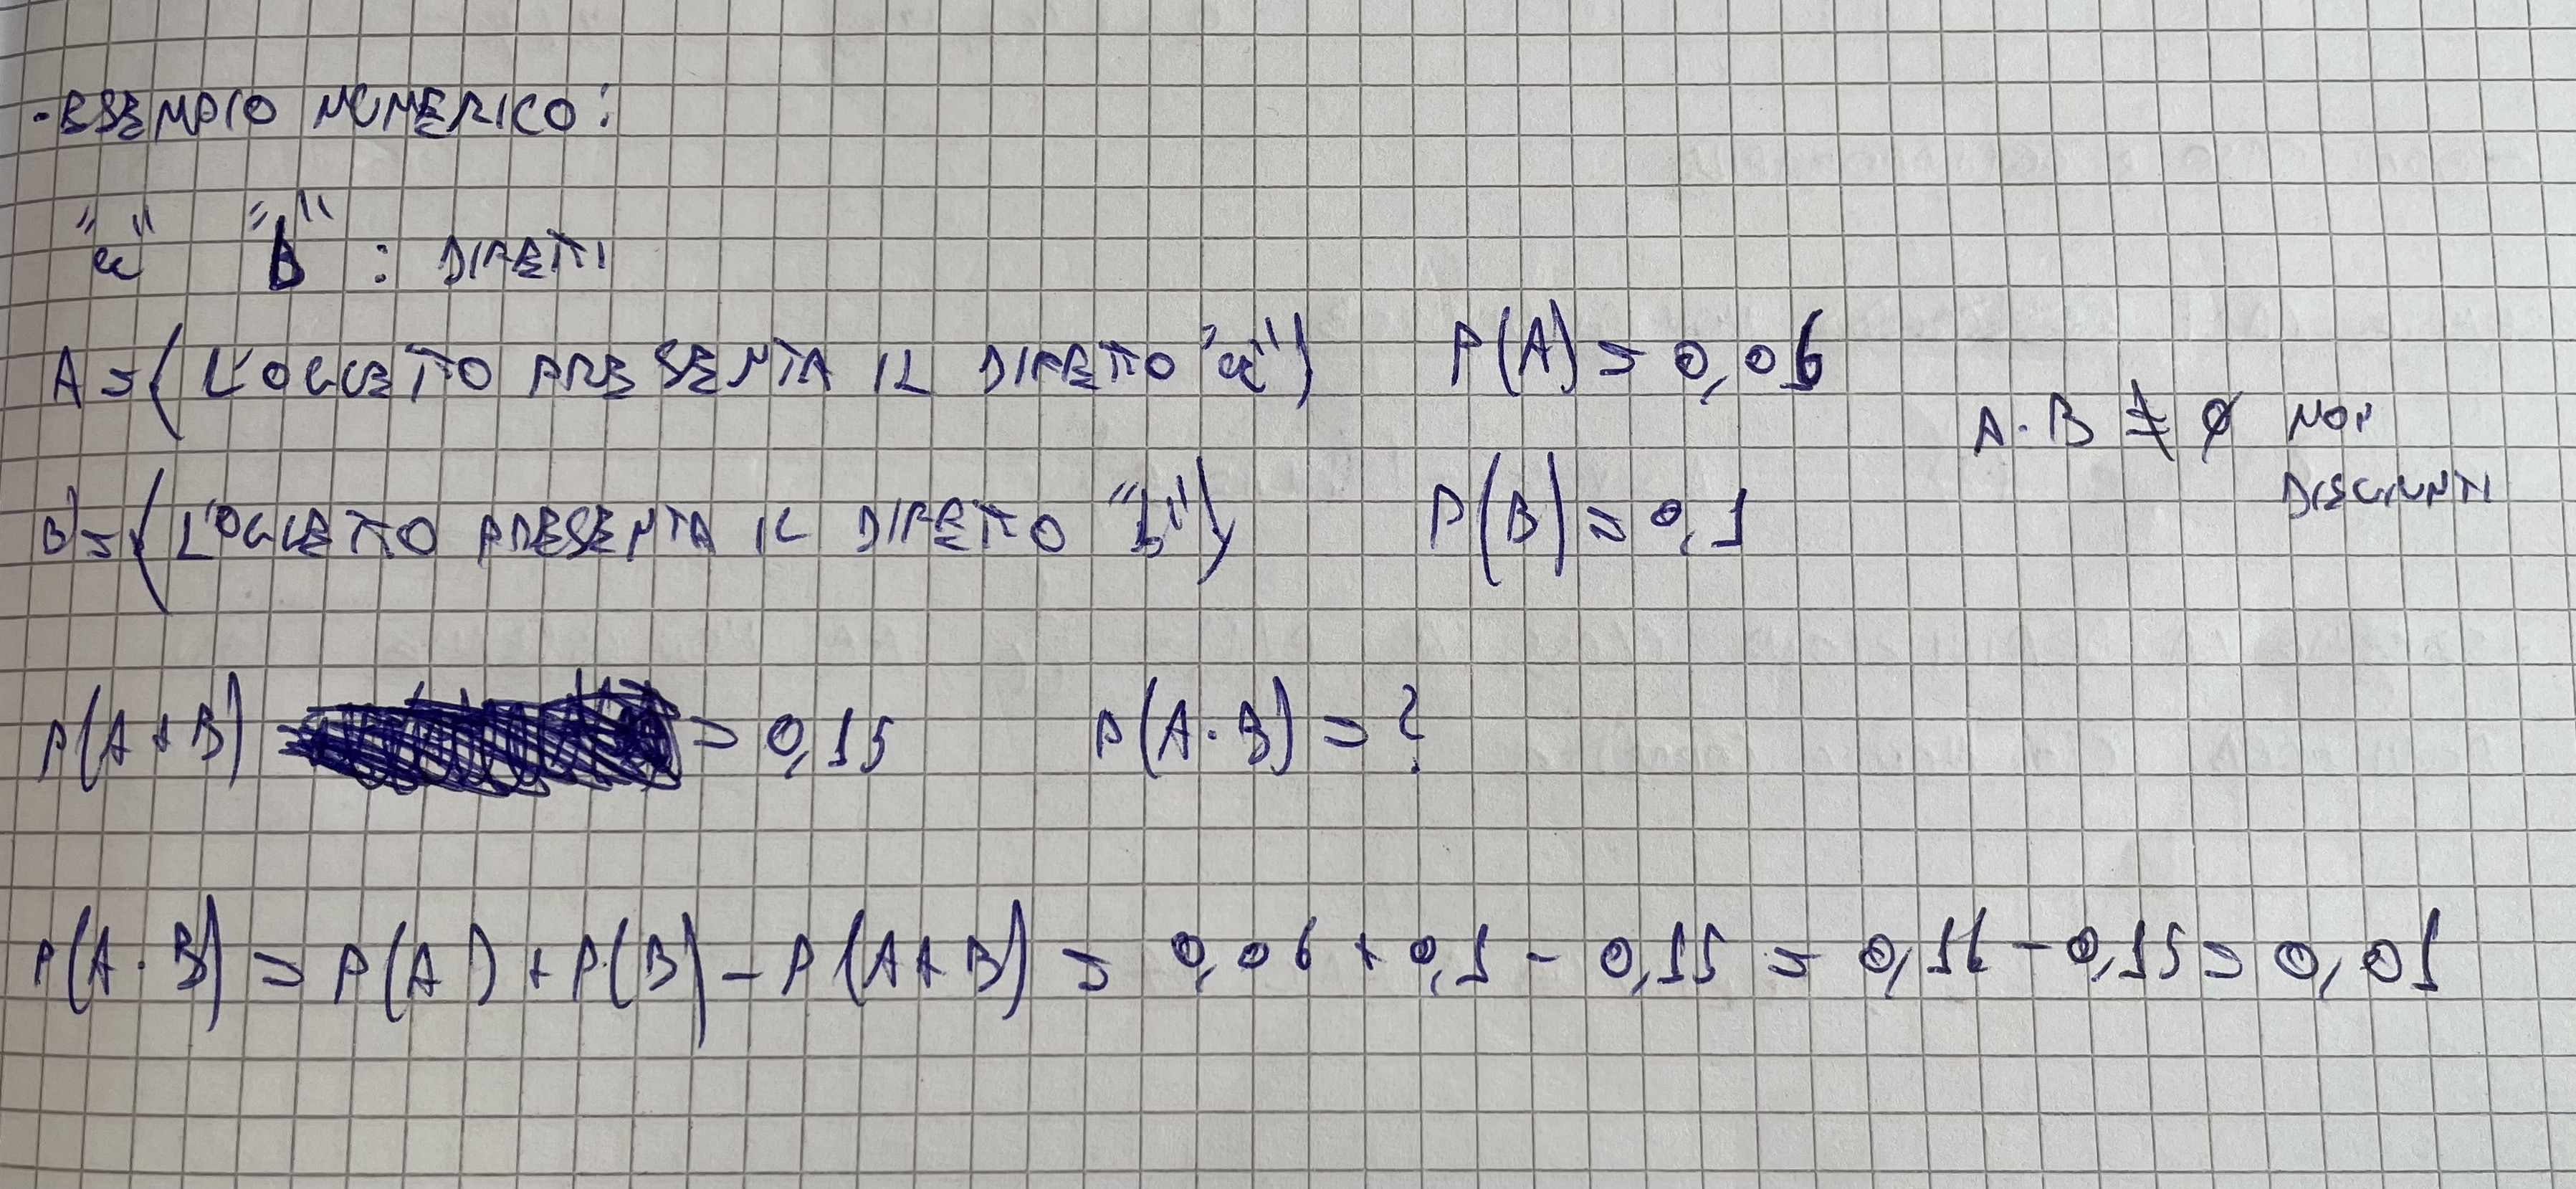
\includegraphics[scale=0.13]{ese/1.jpeg} 
\end{figure}

\begin{figure}[ht]
\centering
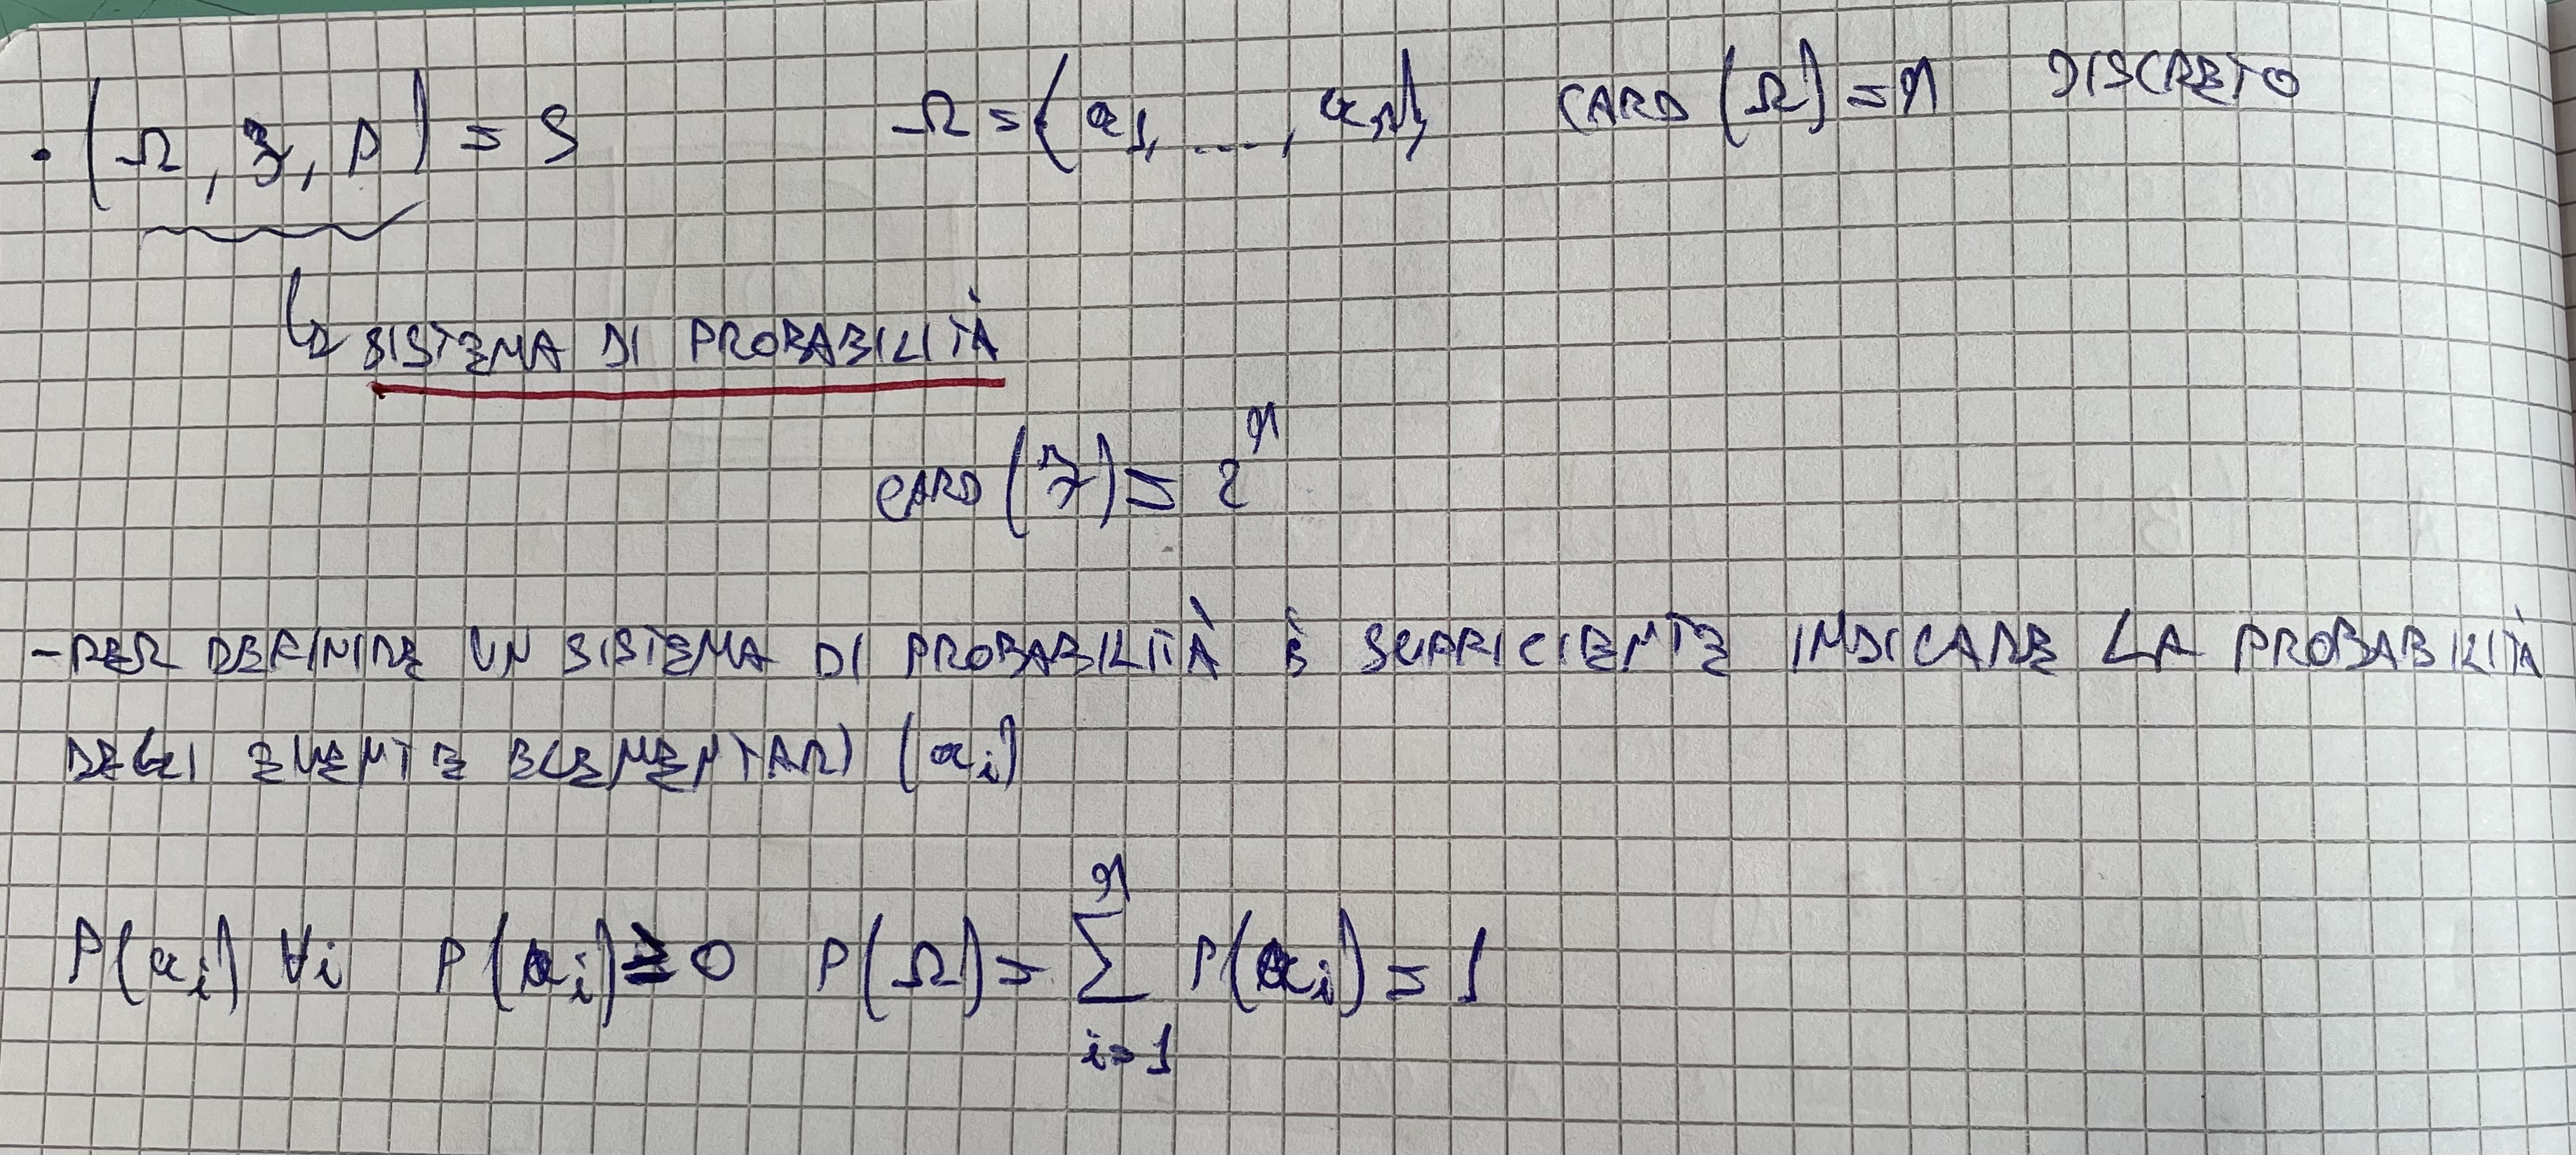
\includegraphics[scale=0.13]{ese/1a.jpeg} 
\end{figure}

\subsection{Sistema di Probabilità}
Definiamo un Sistema di Probabilità come: \\
\begin{tabular}{|p{13cm}}
$S = (\Omega, \mathcal{I}, P)$ dove $\Omega$ è uno spazio campione discreto \\
$\left( \Omega=\{a_1, a_2, \dots, a_n\} \implies Card(\Omega) = n \right)$ e $Card(\mathcal{I}) = 2^n$
\end{tabular} \\ \\
Per definire un sistema di probabilità è sufficiente indicare la probabilità degli eventi elementari $\left( a_i \right)$: \\
$P(a_i) \geq 0 \;\; \forall i=1,2,\dots,n $ \\
$P(\Omega) = \sum_{i=1}^{n} P(a_i) = 1$
\newpage
\subsubsection{\underline{Esempio (Lancio di un dado}}
\begin{figure}[ht]
\centering
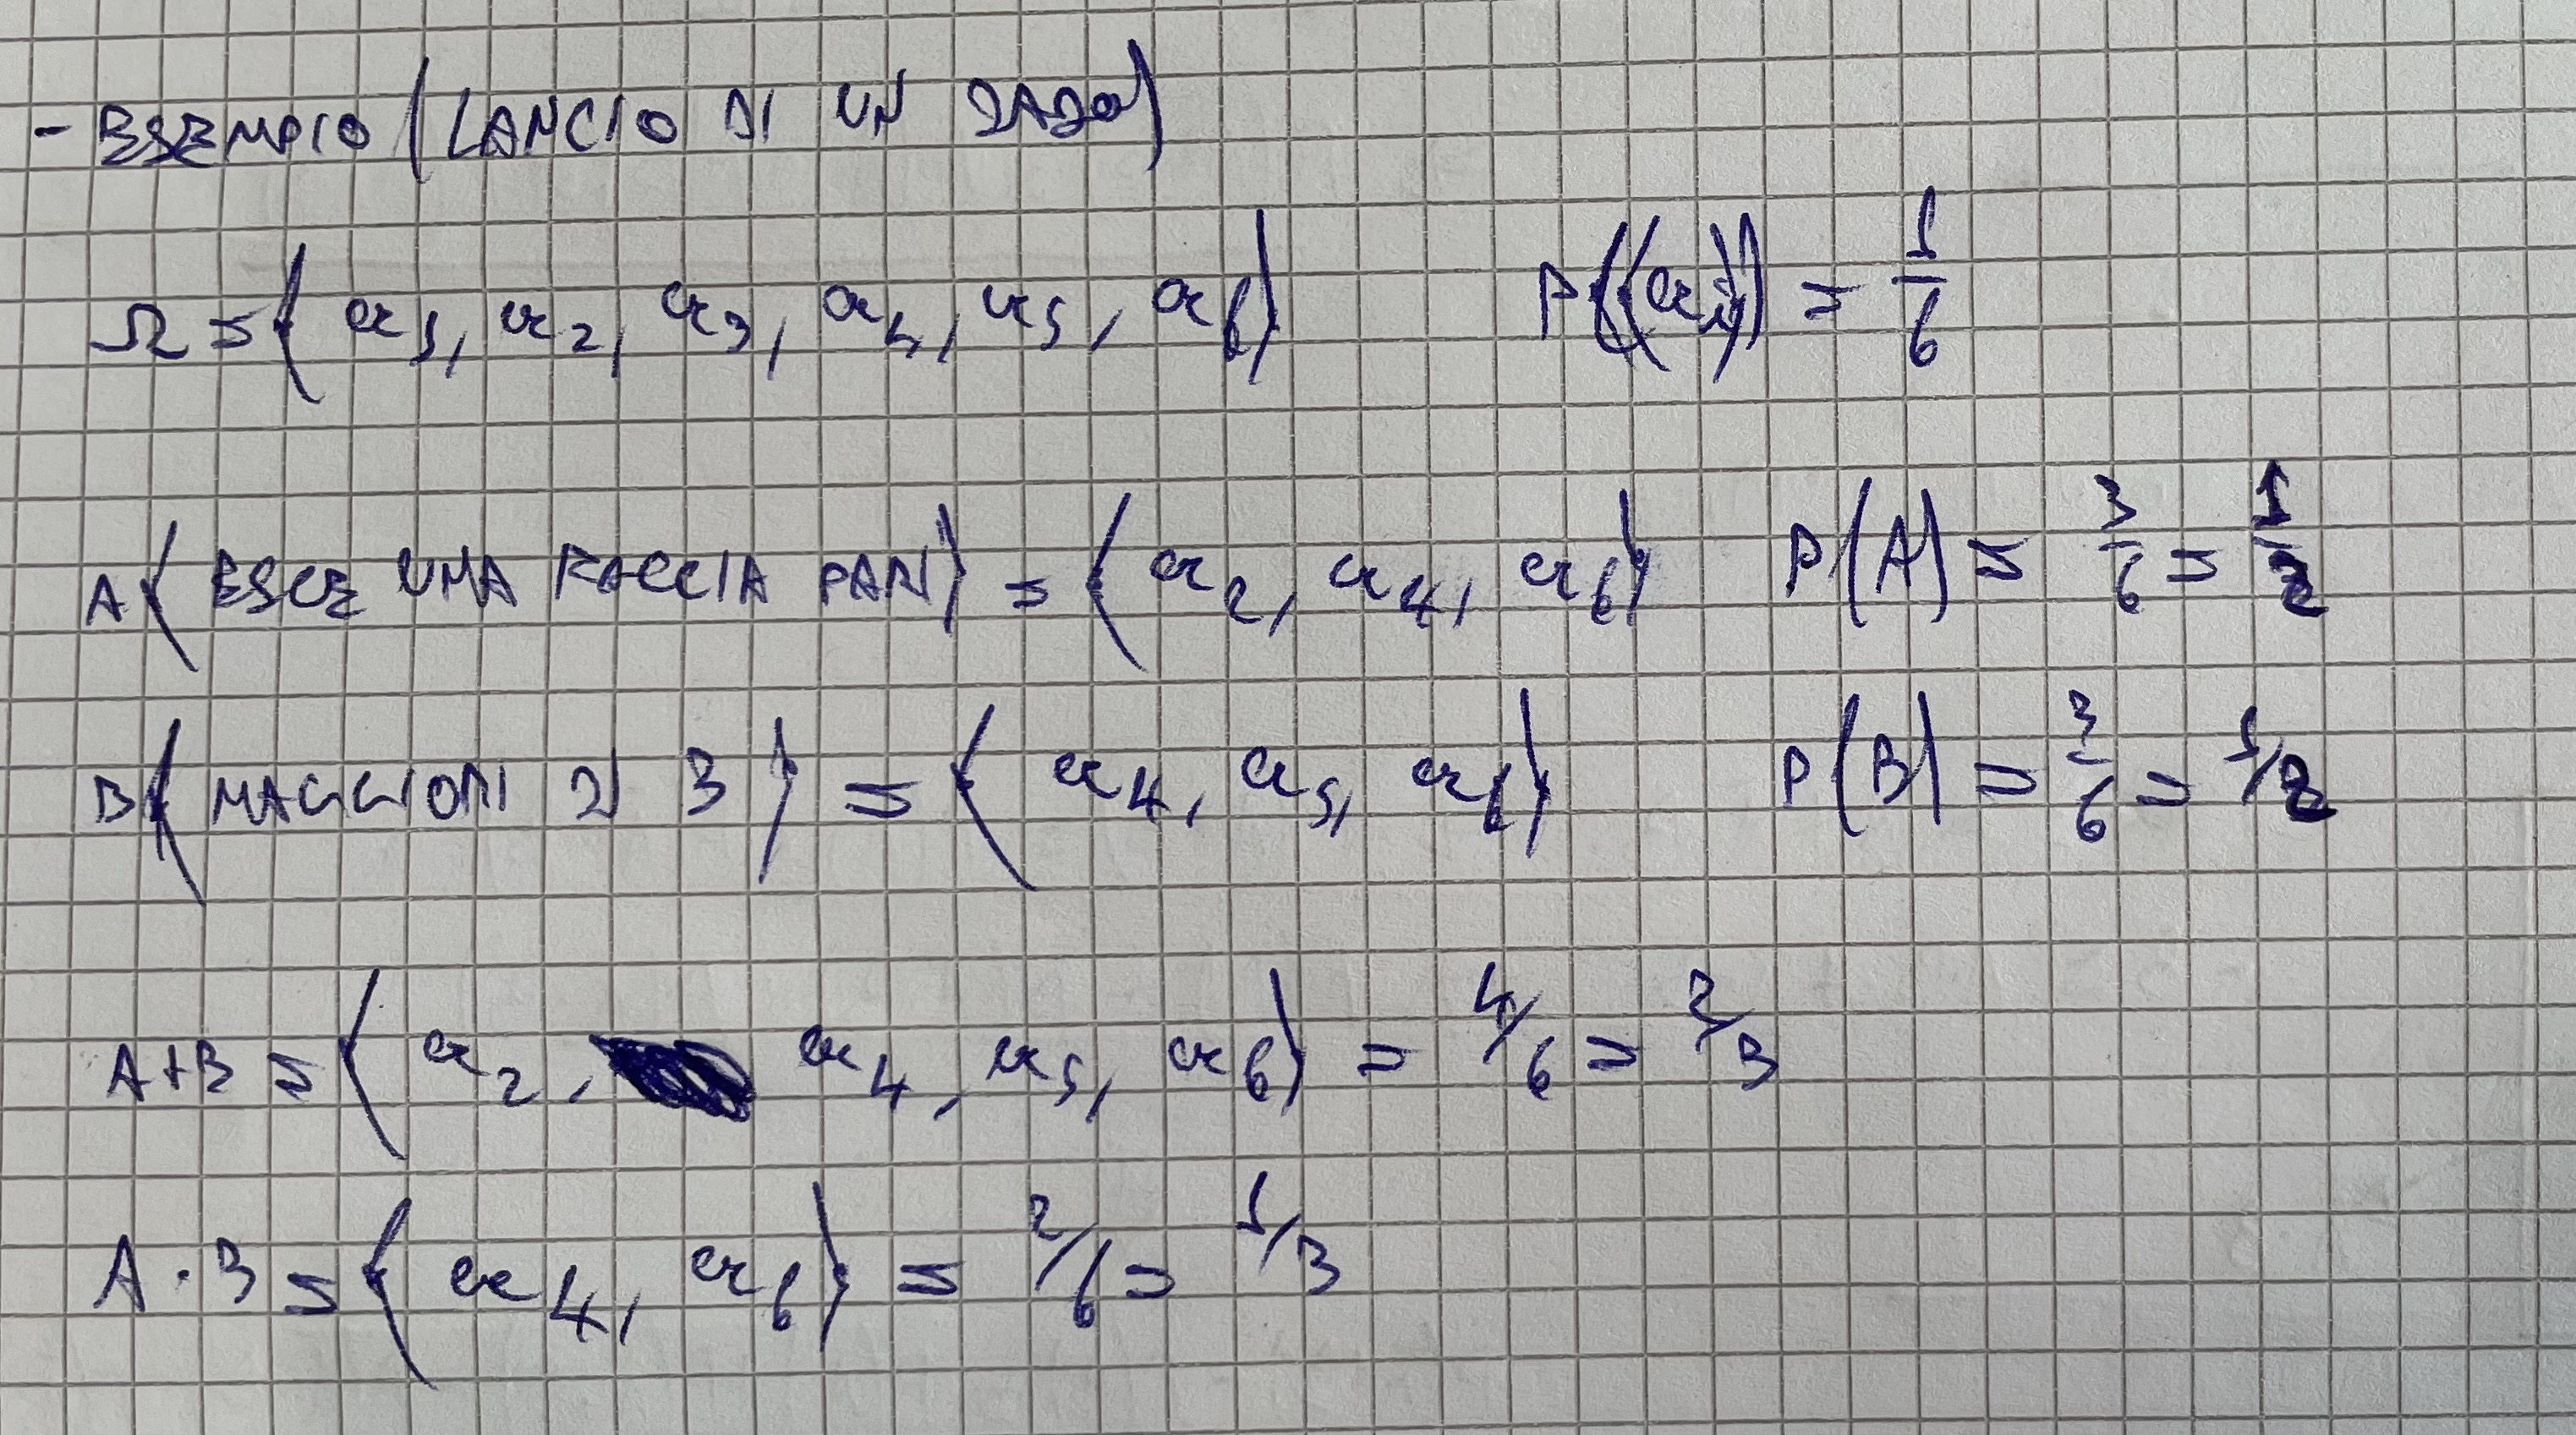
\includegraphics[scale=0.13]{ese/2.jpeg} 
\end{figure}

\subsection{Definizione Classica di Probabilità}
La definizione classica di probabilità la delimitiamo come: $P(A) = \frac{k_A}{k} = \frac{\text{Casi Favorevoli}}{\text{Casi Possibili}}
$
\subsection{Calcolare Probabilità su Spazio Campione Discreto}
Generalmente ci sono 3 modi con cui è possibile calcolare la probabilità in uno spazio campione discreto:
\subsubsection{\underline{Caso Equiprobabile}}
Il caso equiprobabile è il più semplice, poiché basta applicare la definizione classica, per comprendere meglio basta vedere l’esempio seguente.
\paragraph{\underline{Esempio(Lancio dado)}}
$\Omega= \{a_1, a_2, a_3, a_4, a_5, a_6 \} \; \big| \; A= \{ a_2, a_4, a_6\}$ \\
$P(A) = \frac{3}{6} = \frac 12$

\subsubsection{\underline{Caso non Equiprobabile}}
Per spiegare questo caso ci avvarremo di un esempio: \\
$\Omega = \{\text{Numeri da 2 a 12}\} = \{2, 3, \dots, 12 \} $ \\
$A = \{\text{Gli elementi } a_{ij}\text{ la quale somma dei pedici fa } 5\} = \{ a_{ij} \big| i+j = 5\}$ \\ \\
Secondo la definizione classica $P(A) = \frac{1}{11}$, ma non essendo i casi equiprobabili ciò non è corretto e quindi non possiamo applicare la definizione classica di probabilità cosi com’è. \\ \\
Quindi per risolvere questo problema, dobbiamo prima capire quali sono i casi possibili e quali i casi favorevoli.
Per farlo possiamo avvalerci di una matrice in cui evidenzieremo in rosso tutti i casi in cui $i+j = 5$: 
\[\begin{bmatrix}
a_{11} & a_{12} & a_{13} & \color{red}a_{14} & a_{15} & a_{16} \\
a_{21} & a_{22} & \color{red}a_{23} & a_{24} & a_{25} & a_{26} \\
a_{31} & \color{red}a_{32} & a_{33} & a_{34} & a_{35} & a_{36} \\
\color{red}a_{41} & a_{42} & a_{43} & a_{44} & a_{45} & a_{46} \\
a_{51} & a_{52} & a_{53} & a_{54} & a_{55} & a_{56} \\
a_{61} & a_{62} & a_{63} & a_{64} & a_{65} & a_{66} \\
\end{bmatrix}\]
Quindi, i casi totali sono 36 e i casi favorevoli sono 4. \\
Allora possiamo concludere che $P(A) = \frac{4}{36} = \frac{1}{9}$

\subsubsection{\underline{Caso Generico}}
Per spiegare il caso generico è meglio avvalersi di alcuni esempi.
\paragraph{\underline{Esempio 1}}
$n \text{ Diodi } \big|\; n_1 \text{ Diodi difettosi } \big|\; n_1 < n$ \\
$A = \{\text{Estraggo } k \text{ diodi, } k_1 \text{ sono difettosi}\}$ \\
Calcolare la probabilità di $A$. \\
Quindi, sugli $n$ diodi totali, ne estraggo $k$ e sugli $n_1$ difettosi ne estraggo $k_1$. \\
Essendo i diodi difettosi estratti $k_1$, possiamo dedurre che avremo estratto $k-k_1$ diodi non difettosi, quindi possiamo scrivere la probabilità di $A$ come:
\[P(A) = \frac{\left( \begin{matrix} n_1 \\ k_1\end{matrix}\right) \cdot \left(\begin{matrix} n-n_1 \\ k-k_1\end{matrix}\right) }{\left(\begin{matrix} n \\ k\end{matrix}\right)}\]
Dove $\left( \begin{matrix} n_1 \\ k_1\end{matrix}\right)$ sono i casi in cui estraggo solo diodi difettosi. \\
$\left(\begin{matrix} n- n_1 \\ k-k_1\end{matrix}\right)$ invece, sono i casi in cui non estraggo alcun diodo difettoso. \\
Infine $\left(\begin{matrix} n \\ k\end{matrix}\right)$ sono i casi totali.

\paragraph{\underline{Esempio 2}}
Abbiamo un mazzo di carte composto da $n=52$ carte totali. \\
Estraiamo $k=4$ carte dal mazzo, qual è la probabilità che estraendo 4 carte
abbiano tutte un seme diverso? \\
Innanzitutto sappiamo che il mazzo è composto nel seguente modo: 
$\begin{cases}
13 \text{ carte con seme Cuori} \\
13 \text{ carte con seme Quadri} \\
13 \text{ carte con seme Fiori} \\
13 \text{ carte con seme Picche} \\
\end{cases}$
Quindi in ogni estrazione, la probabilità di estrarre una carta con un determinato seme è $\left(\begin{matrix} 13 \\ 1\end{matrix}\right)$ \\
Allora possiamo scrivere la probabilità di $A$ è: \\
$P(A) = \frac{\left(\begin{matrix} 13 \\ 1\end{matrix}\right) \cdot \left(\begin{matrix} 13 \\ 1\end{matrix}\right) \cdot \left(\begin{matrix} 13 \\ 1\end{matrix}\right) \cdot \left(\begin{matrix} 13 \\ 1\end{matrix}\right)} {\left(\begin{matrix} 52 \\ 4\end{matrix}\right)}$ \\
Espandendo le combinazioni otteniamo: \\
$= \frac {\frac{13!}{1! \cdot (13-1)!} \cdot \frac{13!}{1! \cdot (13-1)!} \cdot \frac{13!}{1! \cdot (13-1)!} \cdot \frac{13!}{1! \cdot (13-1)!} } {\frac{52!}{4! \cdot (52-4)!}}
= \frac {\frac{13!}{12!} \cdot \frac{13!}{12!} \cdot \frac{13!}{12!} \cdot \frac{13!}{12!} } {\frac{52!}{4! \cdot 48!}}$ \\
$= \frac { \left( \frac{13!}{12!} \right)^4} {\frac{52!}{4! \cdot 48!}}$ \\
Semplificando otteniamo: $= \frac { \left( 13! \right)^4} {\frac{52 \cdot 51 \cdot 50 \cdot 49}{2 \cdot 3 \cdot4}} = 0,105$

\paragraph{\underline{Generalizzando}}
Nel caso più generico, quando abbiamo $n$ oggetti divisi in $\begin{cases}
n_1 \text{ di tipo } 1 \\
n_1 \text{ di tipo } 2 \\
\vdots \\
n_r \text{ di tipo } r \\
\end{cases}$ \\
Decidiamo di estrarne $k$ e ad ogni estrazione abbiamo: $\begin{cases}
k \text{ oggetti estratti, }k_1 \text{ di tipo } 1 \\
k \text{ oggetti estratti, }k_2 \text{ di tipo } 2 \\
\vdots \\
k \text{ oggetti estratti, }k_r \text{ di tipo } r \\
\end{cases}$ \\ \\
Possiamo scrivere la probabilità come: $\color{red} P(A) = \frac{\left(\begin{matrix} n_1 \\ k_1\end{matrix}\right) \cdot \left(\begin{matrix} n_2 \\ k_2\end{matrix}\right) \cdot \dots \cdot \left(\begin{matrix} n_r \\ k_r\end{matrix}\right)} {\left(\begin{matrix} n \\ k\end{matrix}\right)}$

\subsection{Calcolare Probabilità su Spazio Campione Continuo}
Definiamo i seguenti eventi: $A=\{x\in\mathbb{R}\left|x\leq x_1\right\}$ $\forall x_1$ e
${\color{green}B}=\{x\in\mathbb{R}\left|x\leq x_2\right\}\quad x_2>x_1$ \\
\subsubsection{\underline{Grafico}} ~\\
\begin{figure}[ht]
\centering
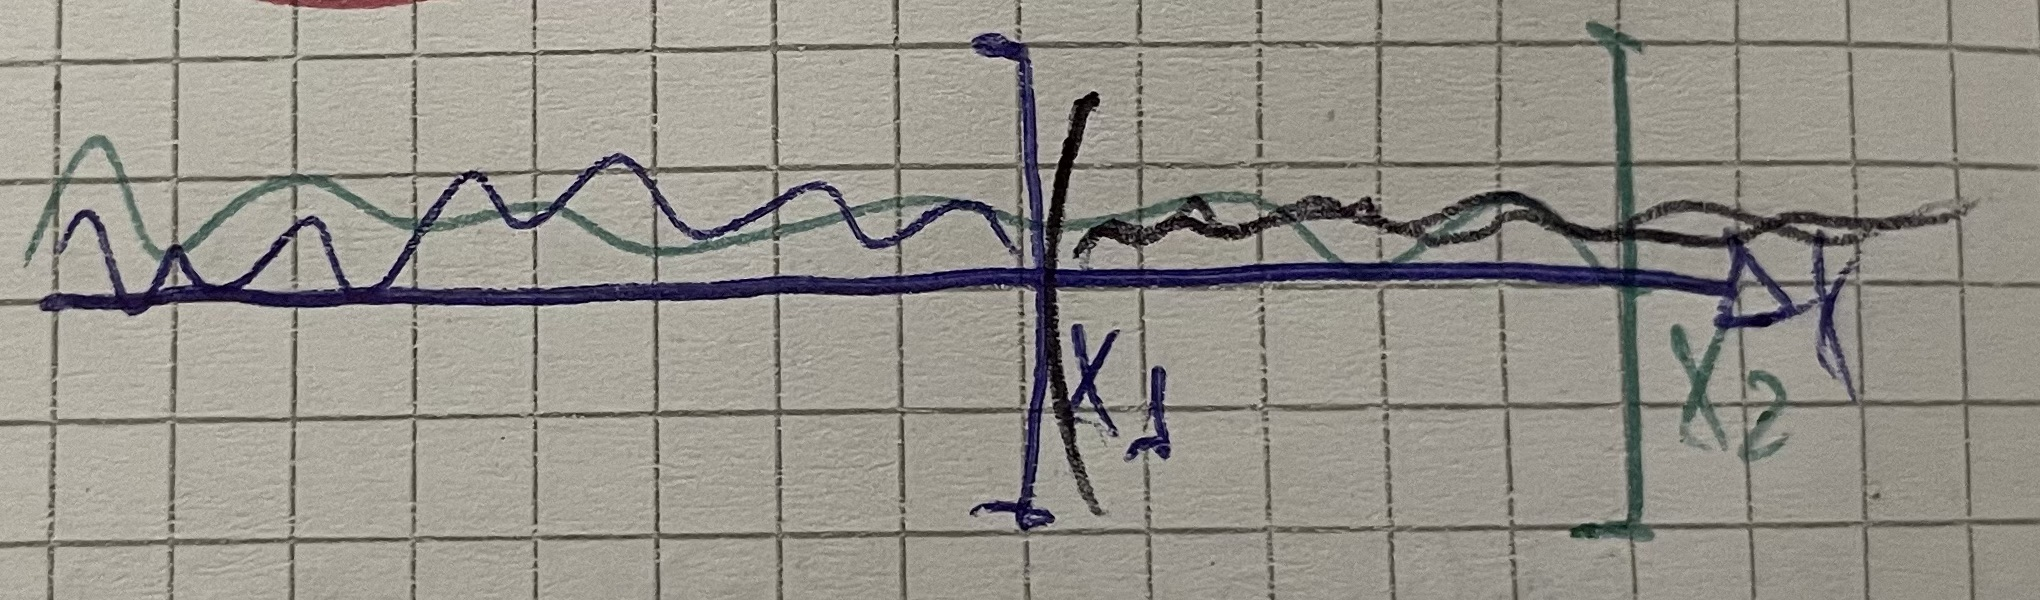
\includegraphics[scale=0.13]{images/23.Par4.9.jpeg} 
\end{figure} \\
Quindi possiamo dedurre che $\overline {A}= \{ x\in \mathbb{R} \left | x> x_1\right \}$e
$\overline{A}\cdot B=\{x\in\mathbb{R}\left|x_1<x<x_2\right\}$ \\
\begin{tabular}{|p{13cm}}
Per aiutarci a calcolare le probabilità di questi eventi, conviene definire un sistema di probabilità, per farlo ci basta definire una funzione $f(x)$ tale che:
\begin{enumerate}
    \item $f(x) \geq 0$
    \item $P(\Omega) = \int_{- \infty}^{+ \infty} f(x) dx = 1$
\end{enumerate}
\end{tabular} \\
Quindi, grazie al sistema di probabilità, possiamo scrivere $P(A)$ come: $P(A) = P\{x \leq x_1 \} = \int_{-\infty}^{x_1} f(x) dx$ \\ \\
Proviamo adesso a calcolare $\overline{A}\cdot B=\{x\in\mathbb{R}\left|x_1<x<x_2\right\}$ che per
comodità chiameremo $C$. \\
Possiamo facilmente dedurre che $A + C = A+ \overline A \cdot B = B \implies P(A) +P(C) = P(B)$ \\
Quindi $P(C) = P(B) - P(A) = \int_{- \infty}^{x_2} f(x) dx - \int_{-\infty}^{x_1} f(x) dx = \int_{x_1}^{x_2} f(x)dx$ \\ \\
Provando a calcolare $P\left(\{x=x_1\}\right)$, si ottiene invece $P\left(\{x=x_1\}\right)=0\to$ equivalente alla probabilità dell'evento impossibile. \\
Questo perché l’integrale risultante non avrebbe estremi. \\
Da questo risulta che: \\
\begin{tabular}{|p{13cm}}
Nel caso degli spazi campione continui, la probabilità di un evento elementare è sempre nulla
\end{tabular}
\subsubsection{\underline{Esempio(Decadimento sostanza radioattiva)}}
\begin{figure}[ht]
\centering
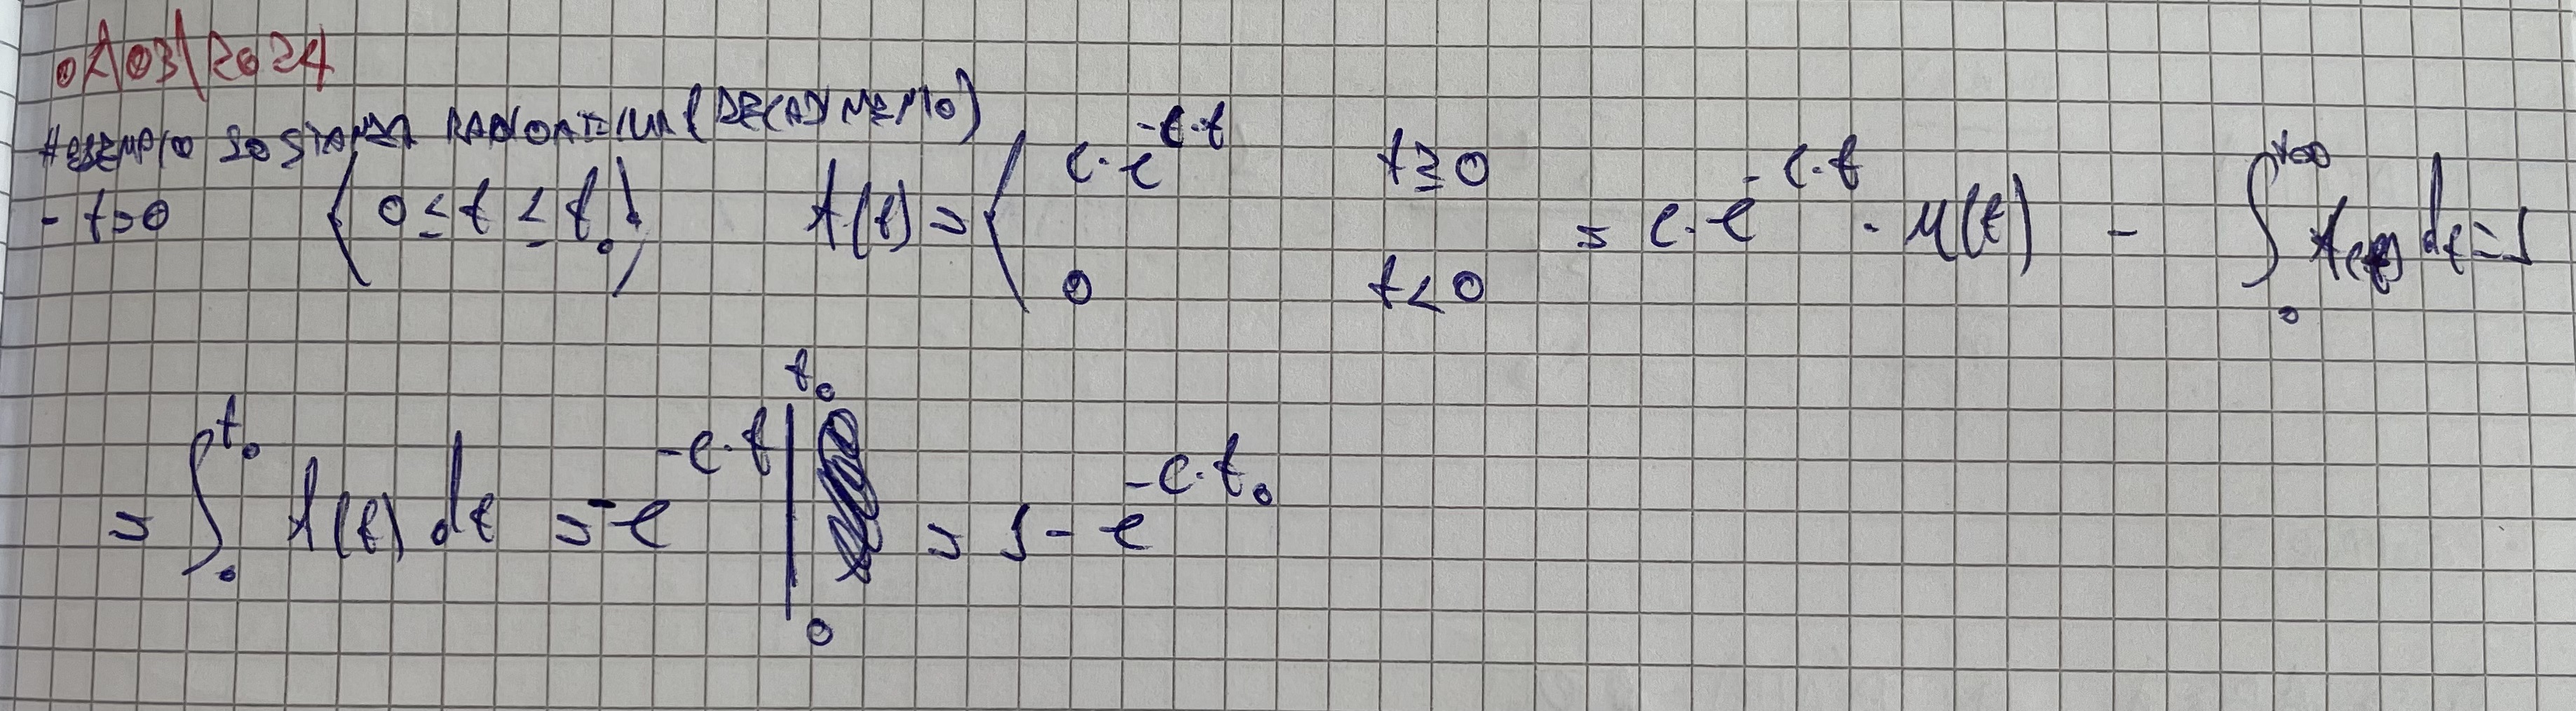
\includegraphics[scale=0.13]{ese/3.jpeg} 
\end{figure}
\newpage
\subsubsection{\underline{Esempio(Telefonata)}}
\begin{figure}[ht]
\centering
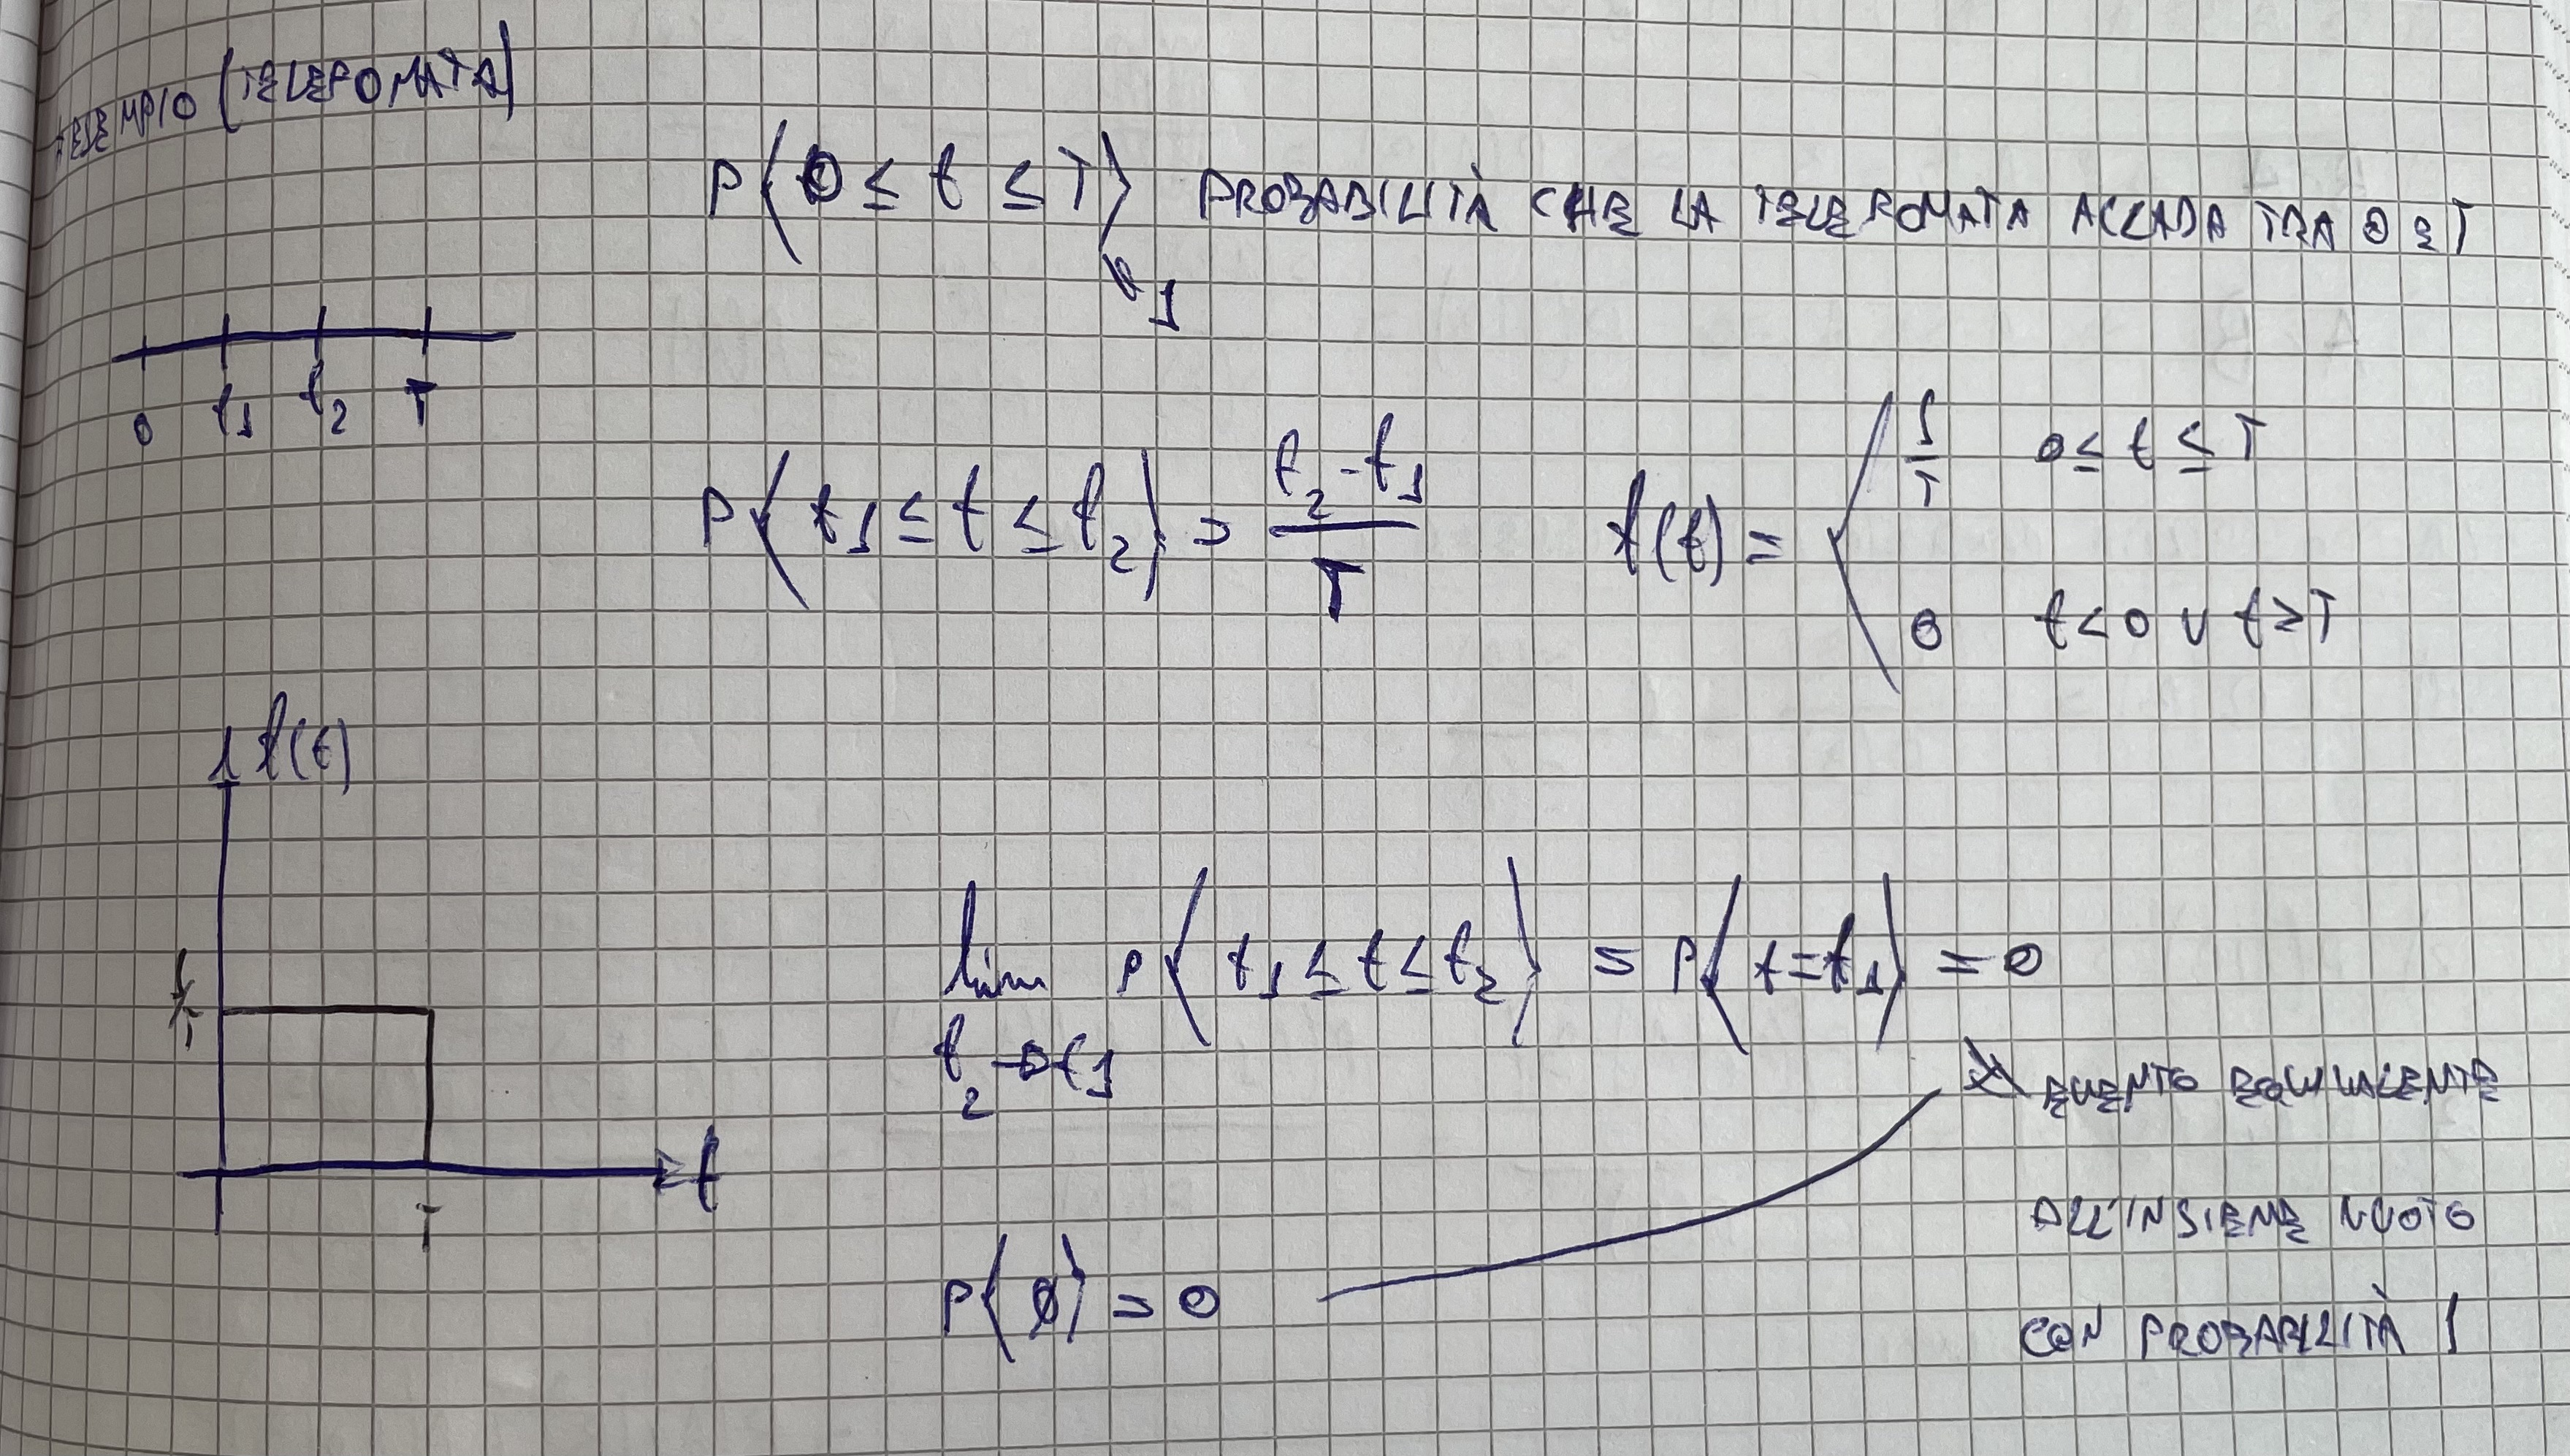
\includegraphics[scale=0.13]{ese/4.jpeg} 
\end{figure}

\subsection{Probabilità Congiunta}
\begin{tabular}{|p{13cm}}
La probabilità congiunta non è altro che la probabilità che avvenga un’intersezione fra due eventi: $P(A \cdot B) = P(A \cap B)$
\end{tabular}

\subsection{Probabilità Condizionata}
\begin{tabular}{|p{13cm}}
Supponiamo che $P(B)\neq0$, allora: \\
$P( A| B) $ è la probabilità di $A$ condizionata a $B$, ovvero la probabilità che al
verificarsi dell'evento $B$ si verifichi anche l'evento $A$. \\ \\
Per calcolare una probabilità condizionata si usa la seguente formula:
\[P(A|B) = \frac{P(A \cdot B)}{P(B)} = \frac{\frac{n(A \cdot B)}{\cancel n}}{\frac{n(B)}{\cancel n}} = \frac{n(A \cdot B)}{n(B)} = \frac{\text{Numero di volte in cui si verifica } A\cdot B}{\text{Numero di volte in cui si verifica } B}\]
\end{tabular}

\subsubsection{\underline{Esempio(Dado)}}
$A = \{a_6\} \implies P(A) = \frac1 6 \;\big|\; B = \{\text{Facce pari}\} = \{a_2,a_4,a_6\} \implies P(B) = \frac3 6 = \frac 1 2$ \\
$A \cdot B = \{a_6\} $ \\
$P(A|B) = \frac{P(A \cdot B)}{P(B)} = \frac{\frac 1 6}{\frac 1 2} = \frac 1 3$

\subsubsection{\underline{Proprietà}}
\begin{itemize}
    \item Se $AB = \phi \implies P(A|B) = 0$
    \item Se $B \subset A \implies A \cdot B = B \implies P(A|B) = \frac{P(AB)}{P(B)} = \frac{\cancel {P(B)}}{\cancel {P(B)}} = 1$
    \item Se $A \subset B \implies A \cdot B = A \implies P(A|B) = \frac{P(AB)}{P(B)} = \frac{P(A)}{P(B)} \geq P(A)$
\end{itemize}

\subsubsection{\underline{La probabilità condizionata rispetta i 3 assiomi fondamentali:}}
\begin{enumerate}
    \item $P(\Omega | B) = \frac{P(\Omega B)}{P(B)} = \frac{P(B)}{P(B)} = 1$
    \item $P(A|B) \geq 0$
    \item $P(A_1+A_2 |B) = \frac{P[(A_1+A_2)\cdot B]}{P(B)} = \frac{P(A_1B) + P(A_2B)}{P(B)} = \frac{P(A_1B)}{P(B)} + \frac{P(A_2B)}{P(B)} = P(A_1|B)+P(A_2|B)$ con $A_1$ e $A_2$ disgiunti. \\
    \[\begin{matrix}
    & & P(\cdot) \\
     & \nearrow & & \\
    \mathcal{I} & && \\
     & \searrow & &\\
    & & P(\cdot |B)
    \end{matrix}\]
\end{enumerate}

\subsection{Eventi Indipendenti}
Due eventi $A$ e $B$ con $P(A)\neq0$ e $P(B)\neq0$ si dicono indipendenti se il verificarsi di uno dei due non altera la probabilità di verificarsi dell'altro. \\
Quindi se $A$ e $B$ sono indipendenti $\implies P(A\cdot B)=P(A)\cdot P(B)$.

\subsubsection{\underline{3 eventi indipendenti}}
Abbiamo 3 eventi indipendenti $A,B,C$, quindi
$P(ABC)=P(A)\cdot P(B)\cdot P(C)$ che sono indipendenti a coppie.

\subsubsection{\underline{n eventi indipendenti}}
$n$ eventi $A_1,A_2...,A_n$ con $P(A_1),...P(A_n)\neq0$ hanno probabilità congiunta
$P(A_1,A_2,...,A_n)$ ed essendo indipendenti a due a due possono essere
scritti come $P(A_1)\cdot P(A_2)\cdot...\cdot P(A_n)$

\subsubsection{\underline{Proprietà}}
\begin{enumerate}
    \item Sappiamo che $P(A+B) = P(A) + P(B) - P(AB)$ \\
    Se invece $A$ e $B$ sono indipendenti $\implies P(A+B)=P(A)+P(B)-P(A)\cdot P(B)$.
    \item Se $A$ e $B$ sono indipendenti, allora anche $\overline{A}$ e $B$ sono indipendenti
    \subsubsection{\underline{Dimostrazione}}
    Possiamo scrivere $B$ come $B = AB + \overline AB$. \\
    Quindi $P(B) = P(AB + \overline AB) = P(AB) + P(\overline AB)$. \\
    $P(\overline AB)$ può essere scritto come: $P(\overline AB) = P(B)-P(AB)$ \\
    Sapendo che $A$ e $B$ sono indipendenti posso scrivere che \\
    $=P(B)-P(A)\cdot P(B)$ \\
    raccogliendo $B$ diventa: \\
    $ = P(B) \cdot \left( 1 - P(A)\right)$ \\
    Infine so che $P(\overline A) = 1 - P(A)$, quindi: \\
    $ = P(B) \cdot  P(\overline A) = P(\overline A B)$ \\
    Dimostrando cosi che anche $\overline{A}$ e $B$ sono indipendenti. 
    \hspace*{0pt}\hfill $\square$ 
    \item Sapendo che $A,B,C$ sono indipendenti $\implies A+B, C $ sono indipendenti 
    \subsubsection{\underline{Dimostrazione}}
    $P[(A+B),C] = P(AC+BC) = P(AC) + P(BC) - P(ABC)$ \\
    Essendo indipendenti posso scrivere che: \\
    $= P(A)\cdot P(C) + P(B)\cdot P(C) - P(A) \cdot P(B) \cdot P(C)$ \\
    Posso raccogliere $P(C)$: \\
    $= P(C) \cdot [P(A) + P(B) - P(A) \cdot P(B)]$ \\
    Ma noi sappiamo che $P(A+B) = P(A) + P(B) - P(A)\cdot P(B)$, quindi: \\
    $= P(C) \cdot P(A+B)$
    \hspace*{0pt}\hfill $\square$
    \item Se $A,B,C $ sono indipendenti $\implies A\cdot B, C $ sono indipendenti
    \subsubsection{\underline{Dimostrazione}}
    $P(ABC) = P(A) \cdot P(B) \cdot P(C)$ \\
    Che possiamo riscrivere come: $= P(AB) \cdot P(C)$
    \hspace*{0pt}\hfill $\square$
\end{enumerate}
\subsubsection{\underline{Esempio(Lancio 2 dadi)}}
\begin{figure}[ht]
\centering
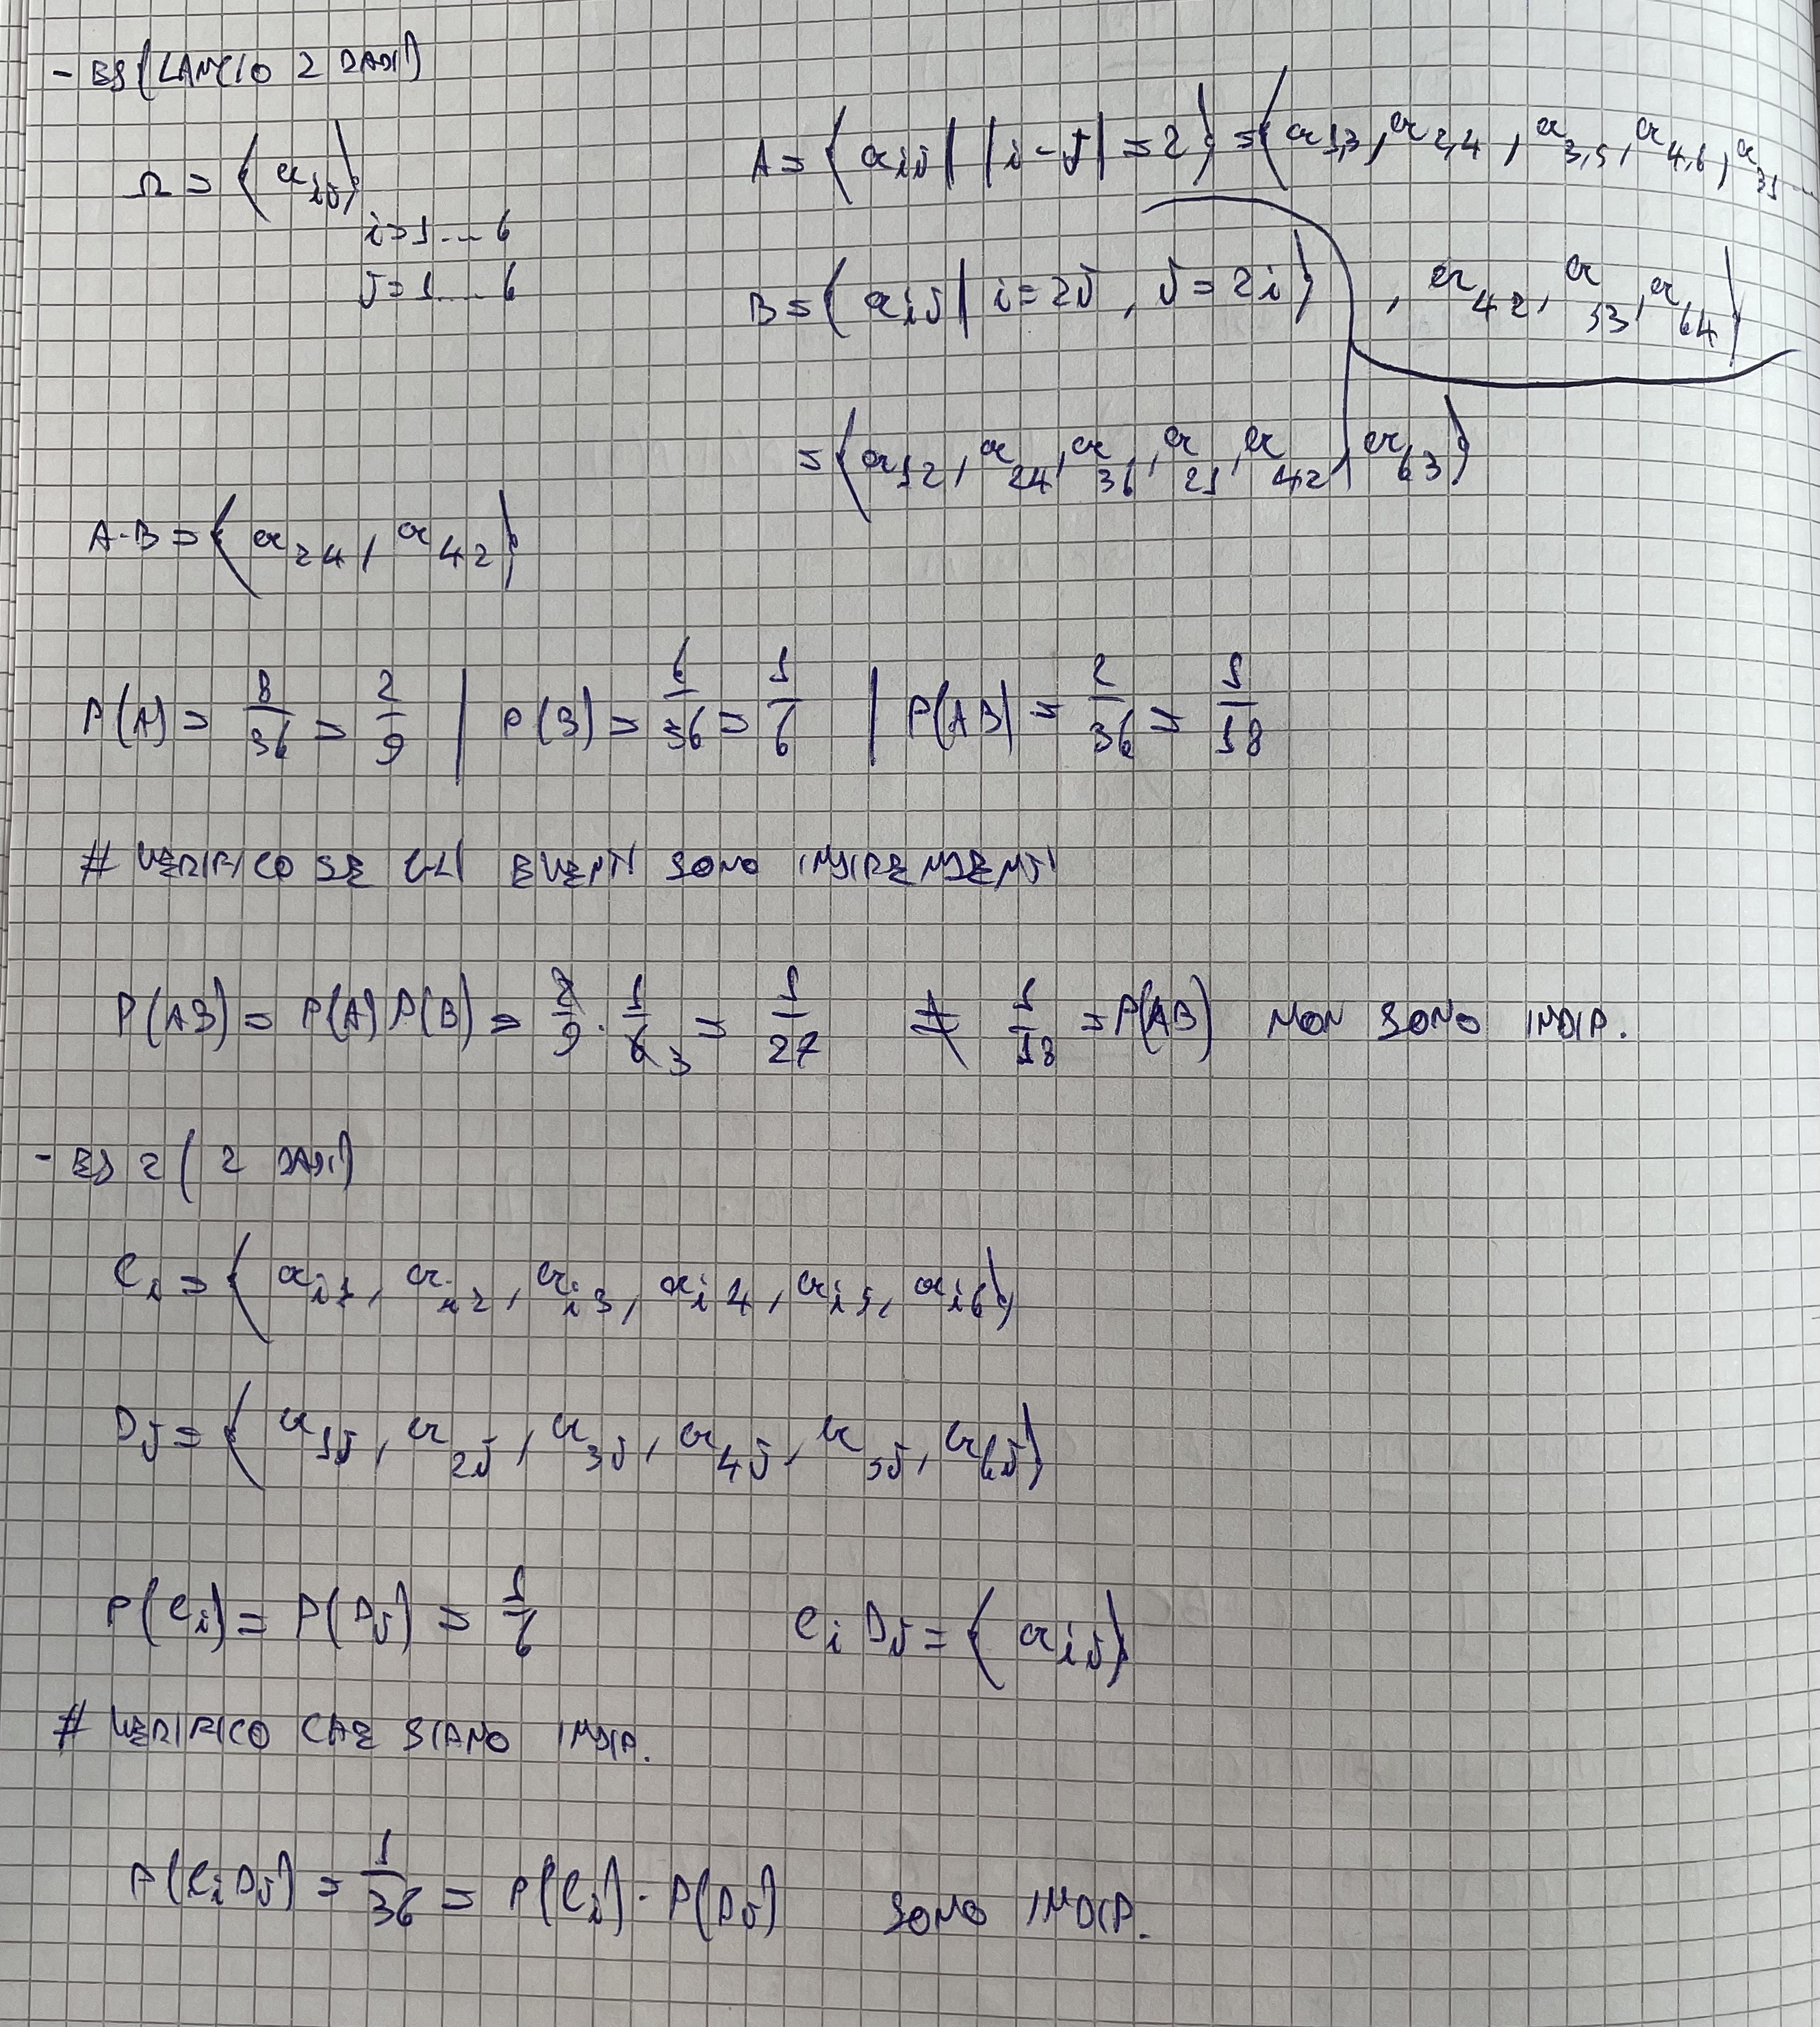
\includegraphics[scale=0.13]{ese/5.jpeg} 
\end{figure}
\begin{figure}[ht]
\centering
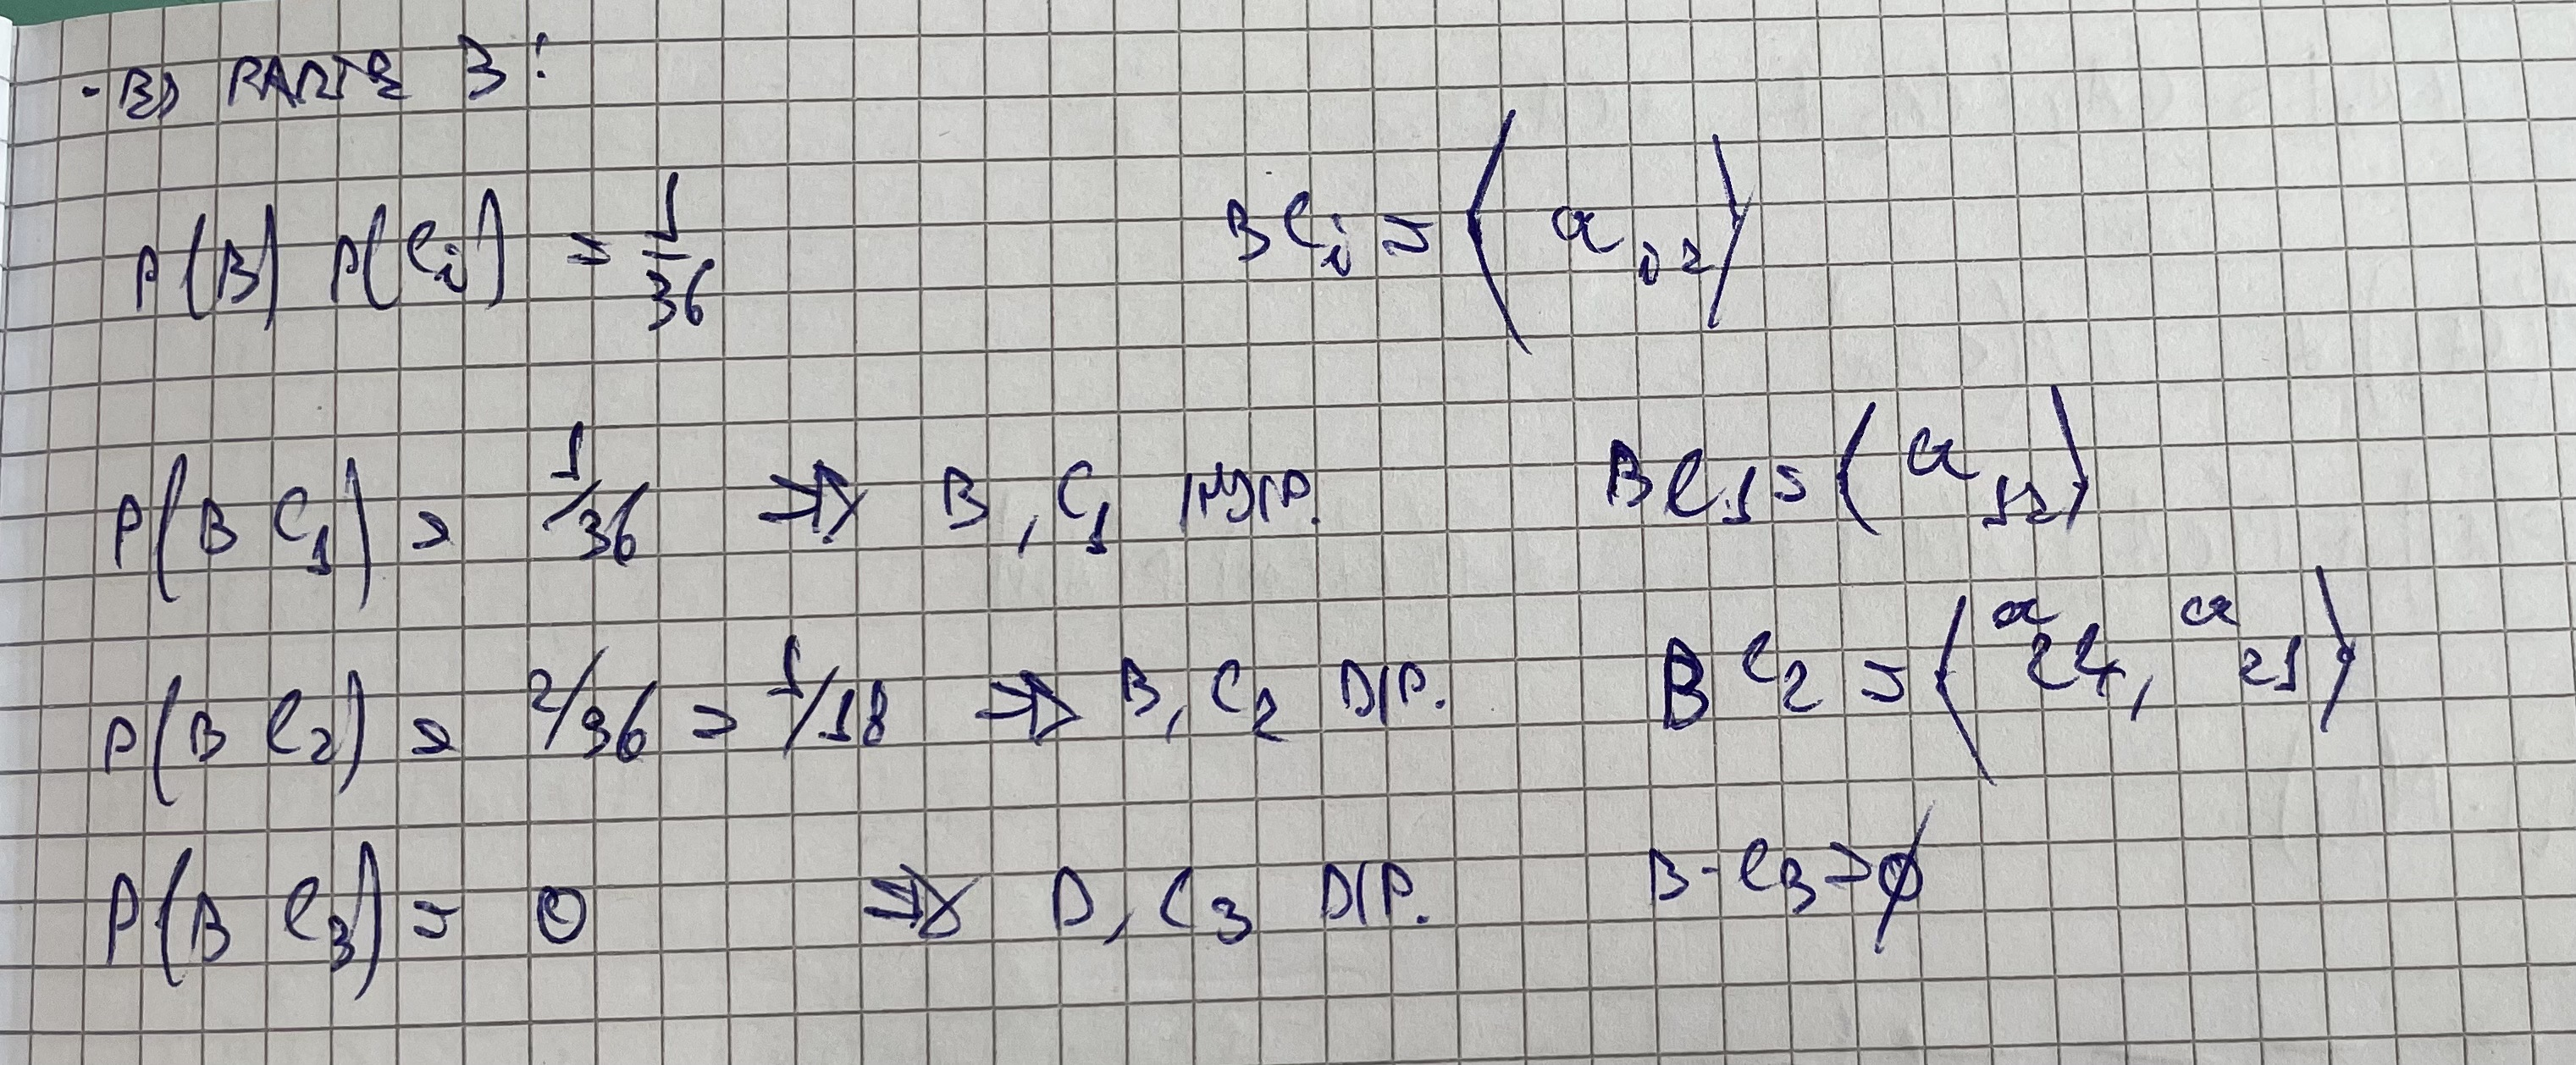
\includegraphics[scale=0.11]{ese/5a.jpeg} 
\end{figure}

\subsection{Probabilità Condizionata con Eventi Indipendenti}
Nel caso in cui due eventi $A$ e $B$ siano indipendenti, la loro probabilità condizionata si calcola così: \\ 
$P(A|B) = \frac{P(AB)}{P(B)} = \frac{P(A) \cdot \cancel{P(B)}}{\cancel{P(B)}} = P(A)$

\subsection{Chain Rule}
\begin{tabular}{|p{13cm}}
La chain rule ci permette di calcolare probabilità congiunte di molteplici eventi grazie all’utilizzo della probabilità condizionata.
\end{tabular}
\subsubsection{\underline{Caso 2/3 eventi}}
$P(A_1|B) = \frac{P(A_1 B)}{P(B)} \implies P(A_1B) = P(A_1 | B) \cdot P(B)$ \\ \\
Se imponiamo $B = A_2 \cdot C$ otteniamo: \\
$= P(A_1A_2C) = P(A_1 |A_2 C) \cdot P(A_2 C)$ \\
Che grazie alla chain rule possiamo scrivere come: \\
$= P(A_1 |A_2 C) \cdot P(A_2 |C) \cdot P(C)$
\subsubsection{\underline{Caso generale, n eventi generici}}
$P(A_1 \cdot A_2 \cdot \dots \cdot A_n) = P(A_1|A_2 \cdot A_3 \cdot \dots \cdot A_n) \cdot P(A_2|A_3 \cdot \dots \cdot A_n) \cdot \dots \cdot P(A_{n-1}| A_n) \cdot P(A_n)$ \\ \\
Che possiamo scrivere come: \\
$P(A_1 \cdot A_2 \cdot \dots \cdot A_n) = P(A_n|A_1 \cdot A_2 \cdot \dots \cdot A_{n-1}) \cdot P(A_{n-1}|A_1 \cdot A_2 \cdot \dots \cdot A_n) \cdot \dots \cdot P(A_2| A_1) \cdot P(A_1)$

\subsection{Teorema di Bayes}
\begin{tabular}{|p{13cm}}
Supponiamo di avere due eventi $A$ e $B$ e di avere una probabilità condizionata $P(A|B) = \frac{P(AB)}{P(B)} \implies P(AB) = P(A|B) \cdot P(B)$ \\
Supponiamo allora di voler calcolare $P(B|A)$, grazie al teorema di Bayes possiamo calcolarla come: $P(B|A) = \frac{P(AB)}{P(A)} = \frac{P(A|B) \cdot P(B)}{P(A)}$ 
\end{tabular} \\
$P(A|B)$ e $P(B|A)$ vengono dette \textbf{probabilità a posteriori}, poiché ci permette di calcolare nel primo caso: la probabilità di $A$, sapendo che si è verificato o che si verificherà con assoluta certezza $B$, e nel secondo: la probabilità di $B$, sapendo che si è verificato o che si verificherà con assoluta certezza $A$. \\
Mentre la probabilità $P(B)$ e la probabilità $P(A)$ si dicono \textbf{probabilità a priori}, poiché non sono condizionate da nessun altro evento o da alcuna conoscenza che potremmo avere sul suo verificarsi. 

\subsection{Teorema della Probabilità Totale}
Siano $A_1,A_2, \dots, A_n$ partizioni di $\Omega \left( \Omega = A_1 + A_2 + \dots + A_n \right)$. \\
$A_1,A_2, \dots, A_n$ incompatibili a due a due, ovvero $A_i \cdot A_j = \phi \;\; \forall i,j$ \\
\begin{figure}[ht]
\centering
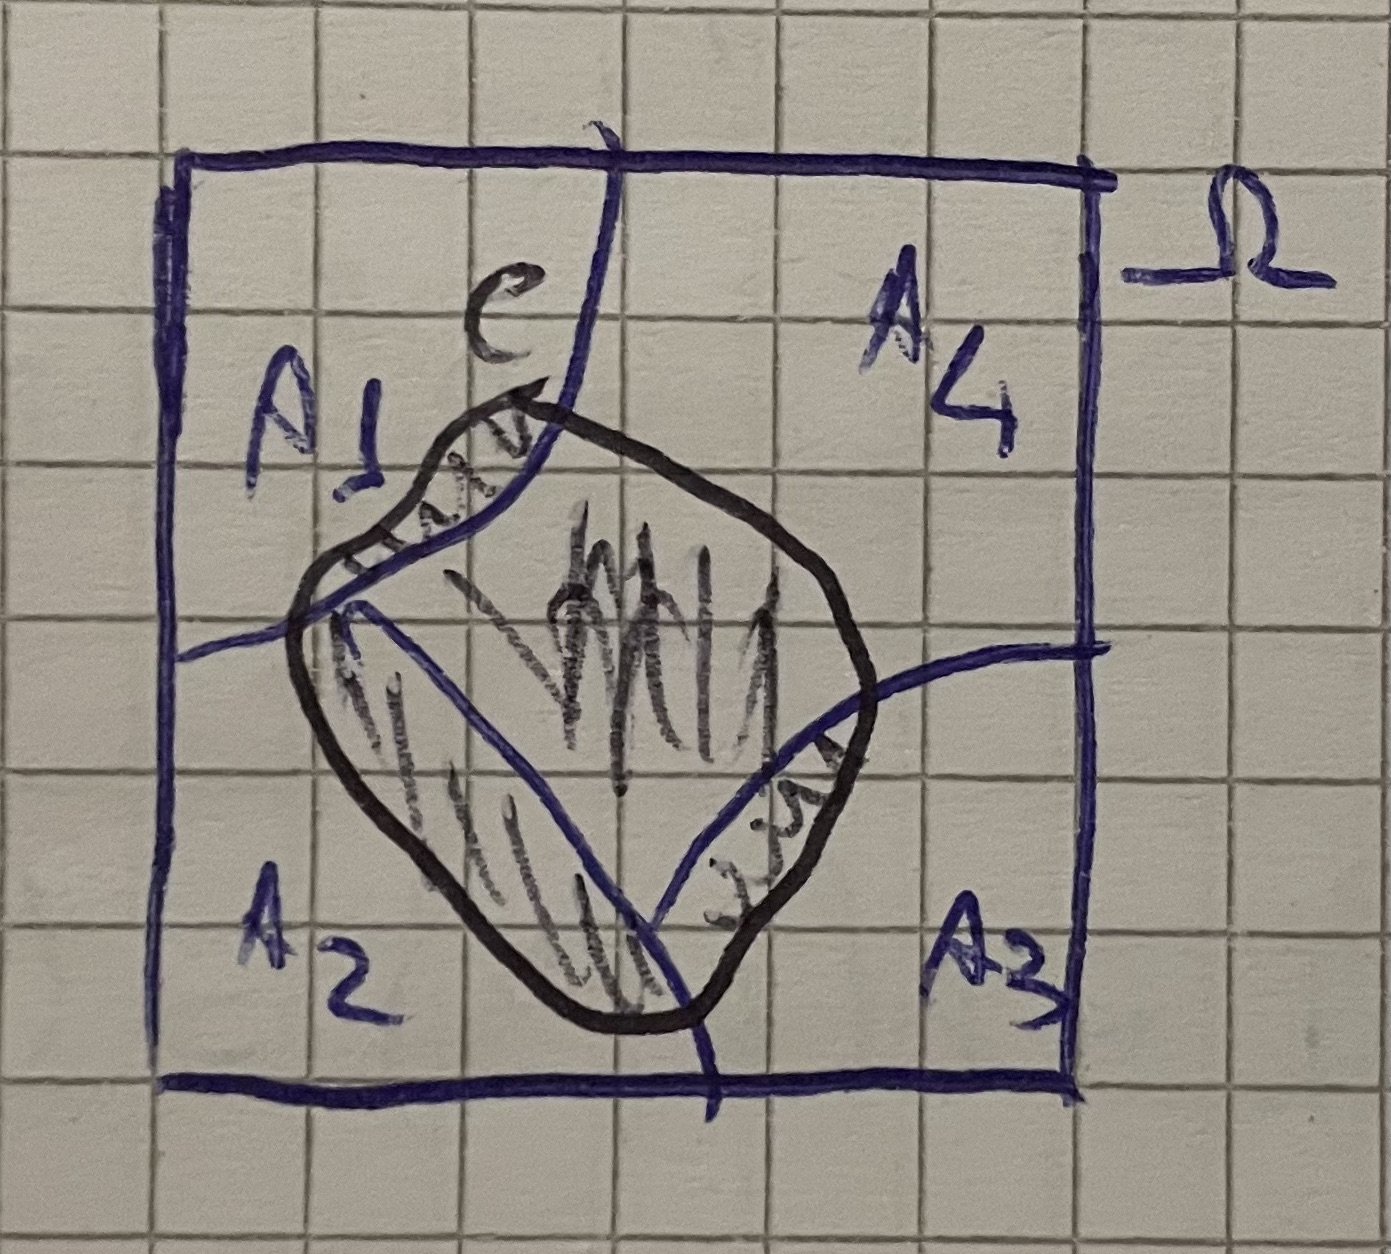
\includegraphics[scale=0.11]{images/24.ProbTot.jpeg}
\end{figure}
$C = C \cdot (A_1 + A_2 + \dots + A_n) = CA_1 +CA_2 + \dots + CA_n$ \\
Quindi la probabilità di $C$ sarà data da: \\
$P(C) = P(CA_1) + P(CA_2) + \dots + P(CA_n)$ \\
Utilizzando il Teorema di Bayes otteniamo: \\
$= P(C|A_1) \cdot P(A_1) + P(C|A_2) \cdot P(A_2) + \dots + P(C|A_n) \cdot P(A_n)$ \\
Possiamo “riassumere” tutto con una sommatoria: 
\[\color{red} \sum_{i=1}^{n} P(C|A_i) \cdot P(A_i)\]
\newpage

\subsection{Composizione Esperimenti Indipendenti} 
\begin{table} [ht]
    \centering
    \begin{tabular}{|c|c|c|}
    \hline
        Esperimento 1 $\varepsilon_1$ & Esperimento 2 $\varepsilon_2$ & Composizione degli esperimenti \\
        \hline
        $\Omega_1$ & $\Omega_2$ & $\Omega = \Omega_1 \times \Omega_1 \left( \text{Prodotto Cartesiano} \right)$\\
        \hline
        $A_1,B_1,C_1, \dots$ & $A_2,B_2,C_2, \dots$ & $A_1 \times A_2, B_1 \times B_2, C_1 \times C_2, \dots$\\
        \hline
        $a_i^{(1)}$ & $a_j^{(2)}$ & $\left( a_i^{(1)} , a_j^{(2)} \right)$\\
        \hline
        $P_1(\cdot)$ & $P_2(\cdot)$ & $P_1(A_1 \times A_2)$\\
        \hline
    \end{tabular}
\end{table} ~\\
Come possiamo ricavare $P(A_1 \times A_2)$? \\
Se gli eventi sono indipendenti posso riscrivere come: $= P_1 \left(A_1 \times \Omega_2 \right) \cdot P_2\left( \Omega_1 \times A_2  \right) $ \\ \\
\begin{tabular}{|p{13cm}}
I due esperimenti $\varepsilon_1$ e $\varepsilon_2$ si dicono indipendenti se il risultato di uno dei due esperimenti non influenza i risultati dell’altro esperimento. \\ \\
Se i due esperimenti NON sono indipendenti, sono vincolato ad eseguire un esperimento prima dell’altro: \\
$P(A_1 \times A_2) = P(A_2 |A_1) = P \left(\Omega_1 \times A_2   \big|  A_1 \times \Omega_2  \right) \cdot P \left(A_1 \times \Omega_2\right)$
\end{tabular}
\subsubsection{\underline{Esempio}}
\begin{figure}[ht]
\centering
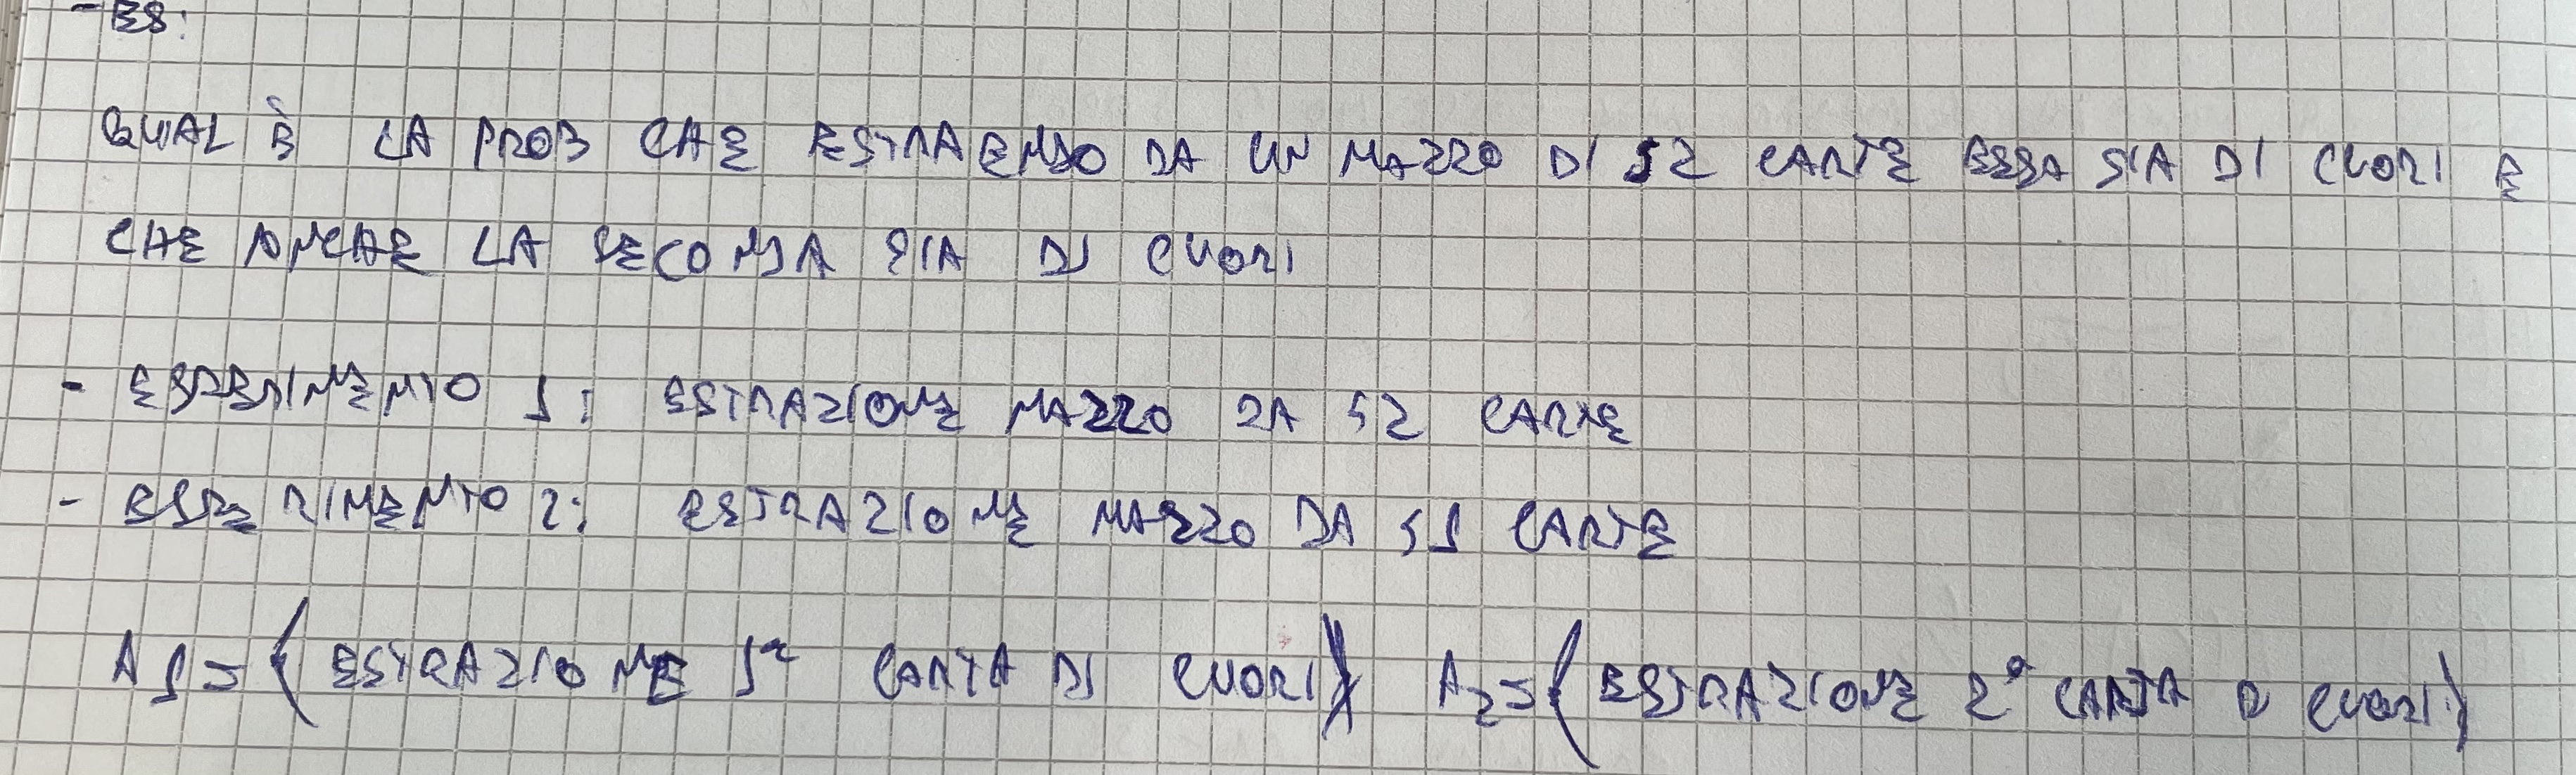
\includegraphics[scale=0.11]{ese/6.jpeg}
\end{figure}
\begin{figure}[ht]
\centering
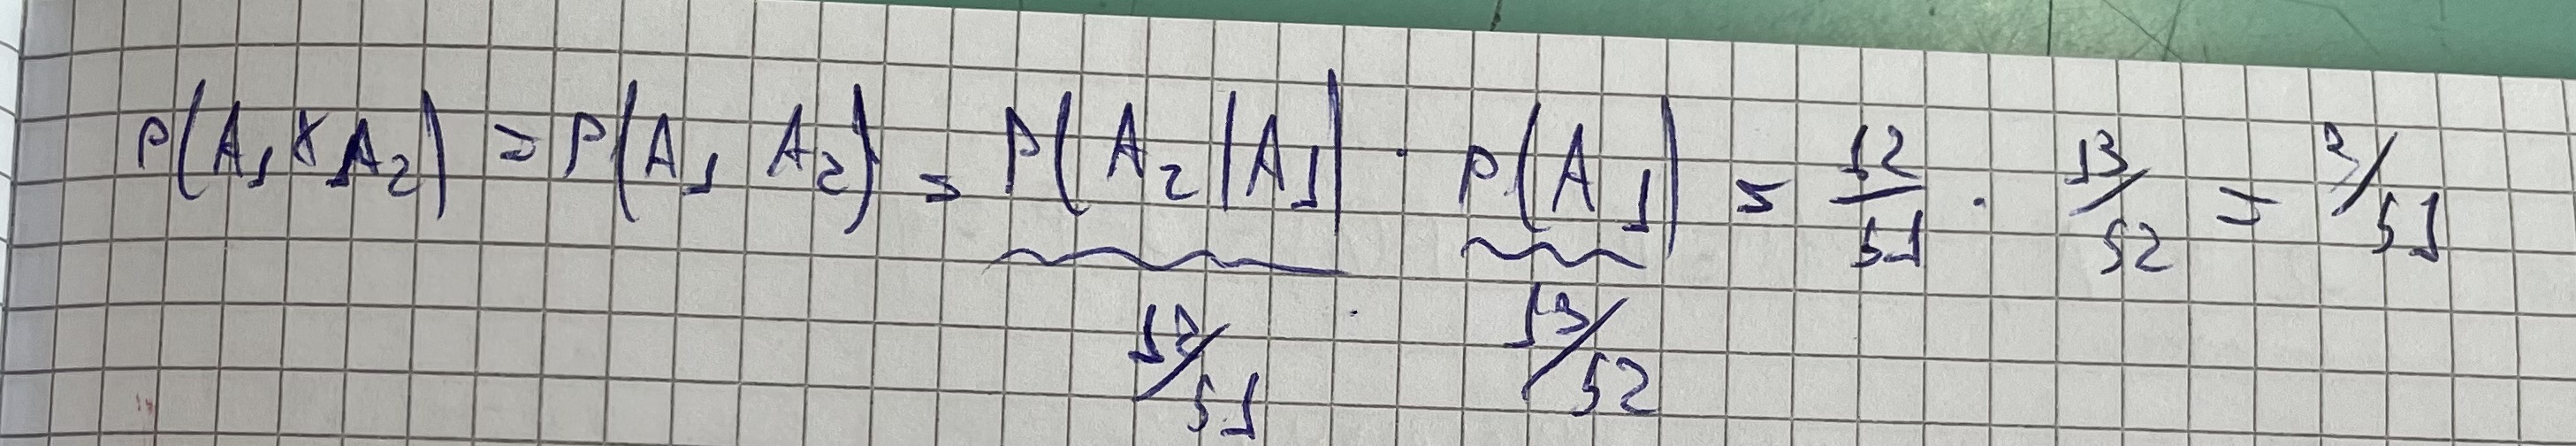
\includegraphics[scale=0.12]{ese/6a.jpeg}
\end{figure}

\subsection{Prove Ripetute (Formula di Bernoulli)}
Primo esperimento: $\Omega  \;\big|\; A \;\big|\; P(A) = p \;\big|\; P(\overline A) = 1-P = q$ \\
Ripetiamo l’esperimento $n$ volte in modo indipendente: $\Omega^{R} = \underset{n}{\underbrace{\Omega \times \Omega \times \dots \times \Omega}}$ \\
$\color{red}P_n(k)$: Probabilità di avere $k$ successi nelle $n$ prove. \\ 
Sia $A_1 = \underset{k}{\underbrace{A \times A \times \dots \times A}} \times \underset{n-k}{\underbrace{\overline A \times \overline A \times  \dots \times  \overline A}}$ tutti eventi disgiunti. \\
Quindi $P(A_1) = p^k \cdot q^{n-k }$ \\
Sia $A_2 = \underset{1}{\underbrace{\overline A}} \times\underset{k}{\underbrace{A \times A \times \dots \times A}} \times \underset{n-k-1}{\underbrace{\overline A \times \overline A \times  \dots \times  \overline A}}$ \\
\begin{tabular}{|p{13cm}}
Possiamo dire che: $P_n(k) = \left( \begin{matrix} n \\ k \end{matrix}\right) \cdot p^k\cdot q^{n-k}$
\end{tabular}
\newpage
\begin{figure}[ht]
\centering
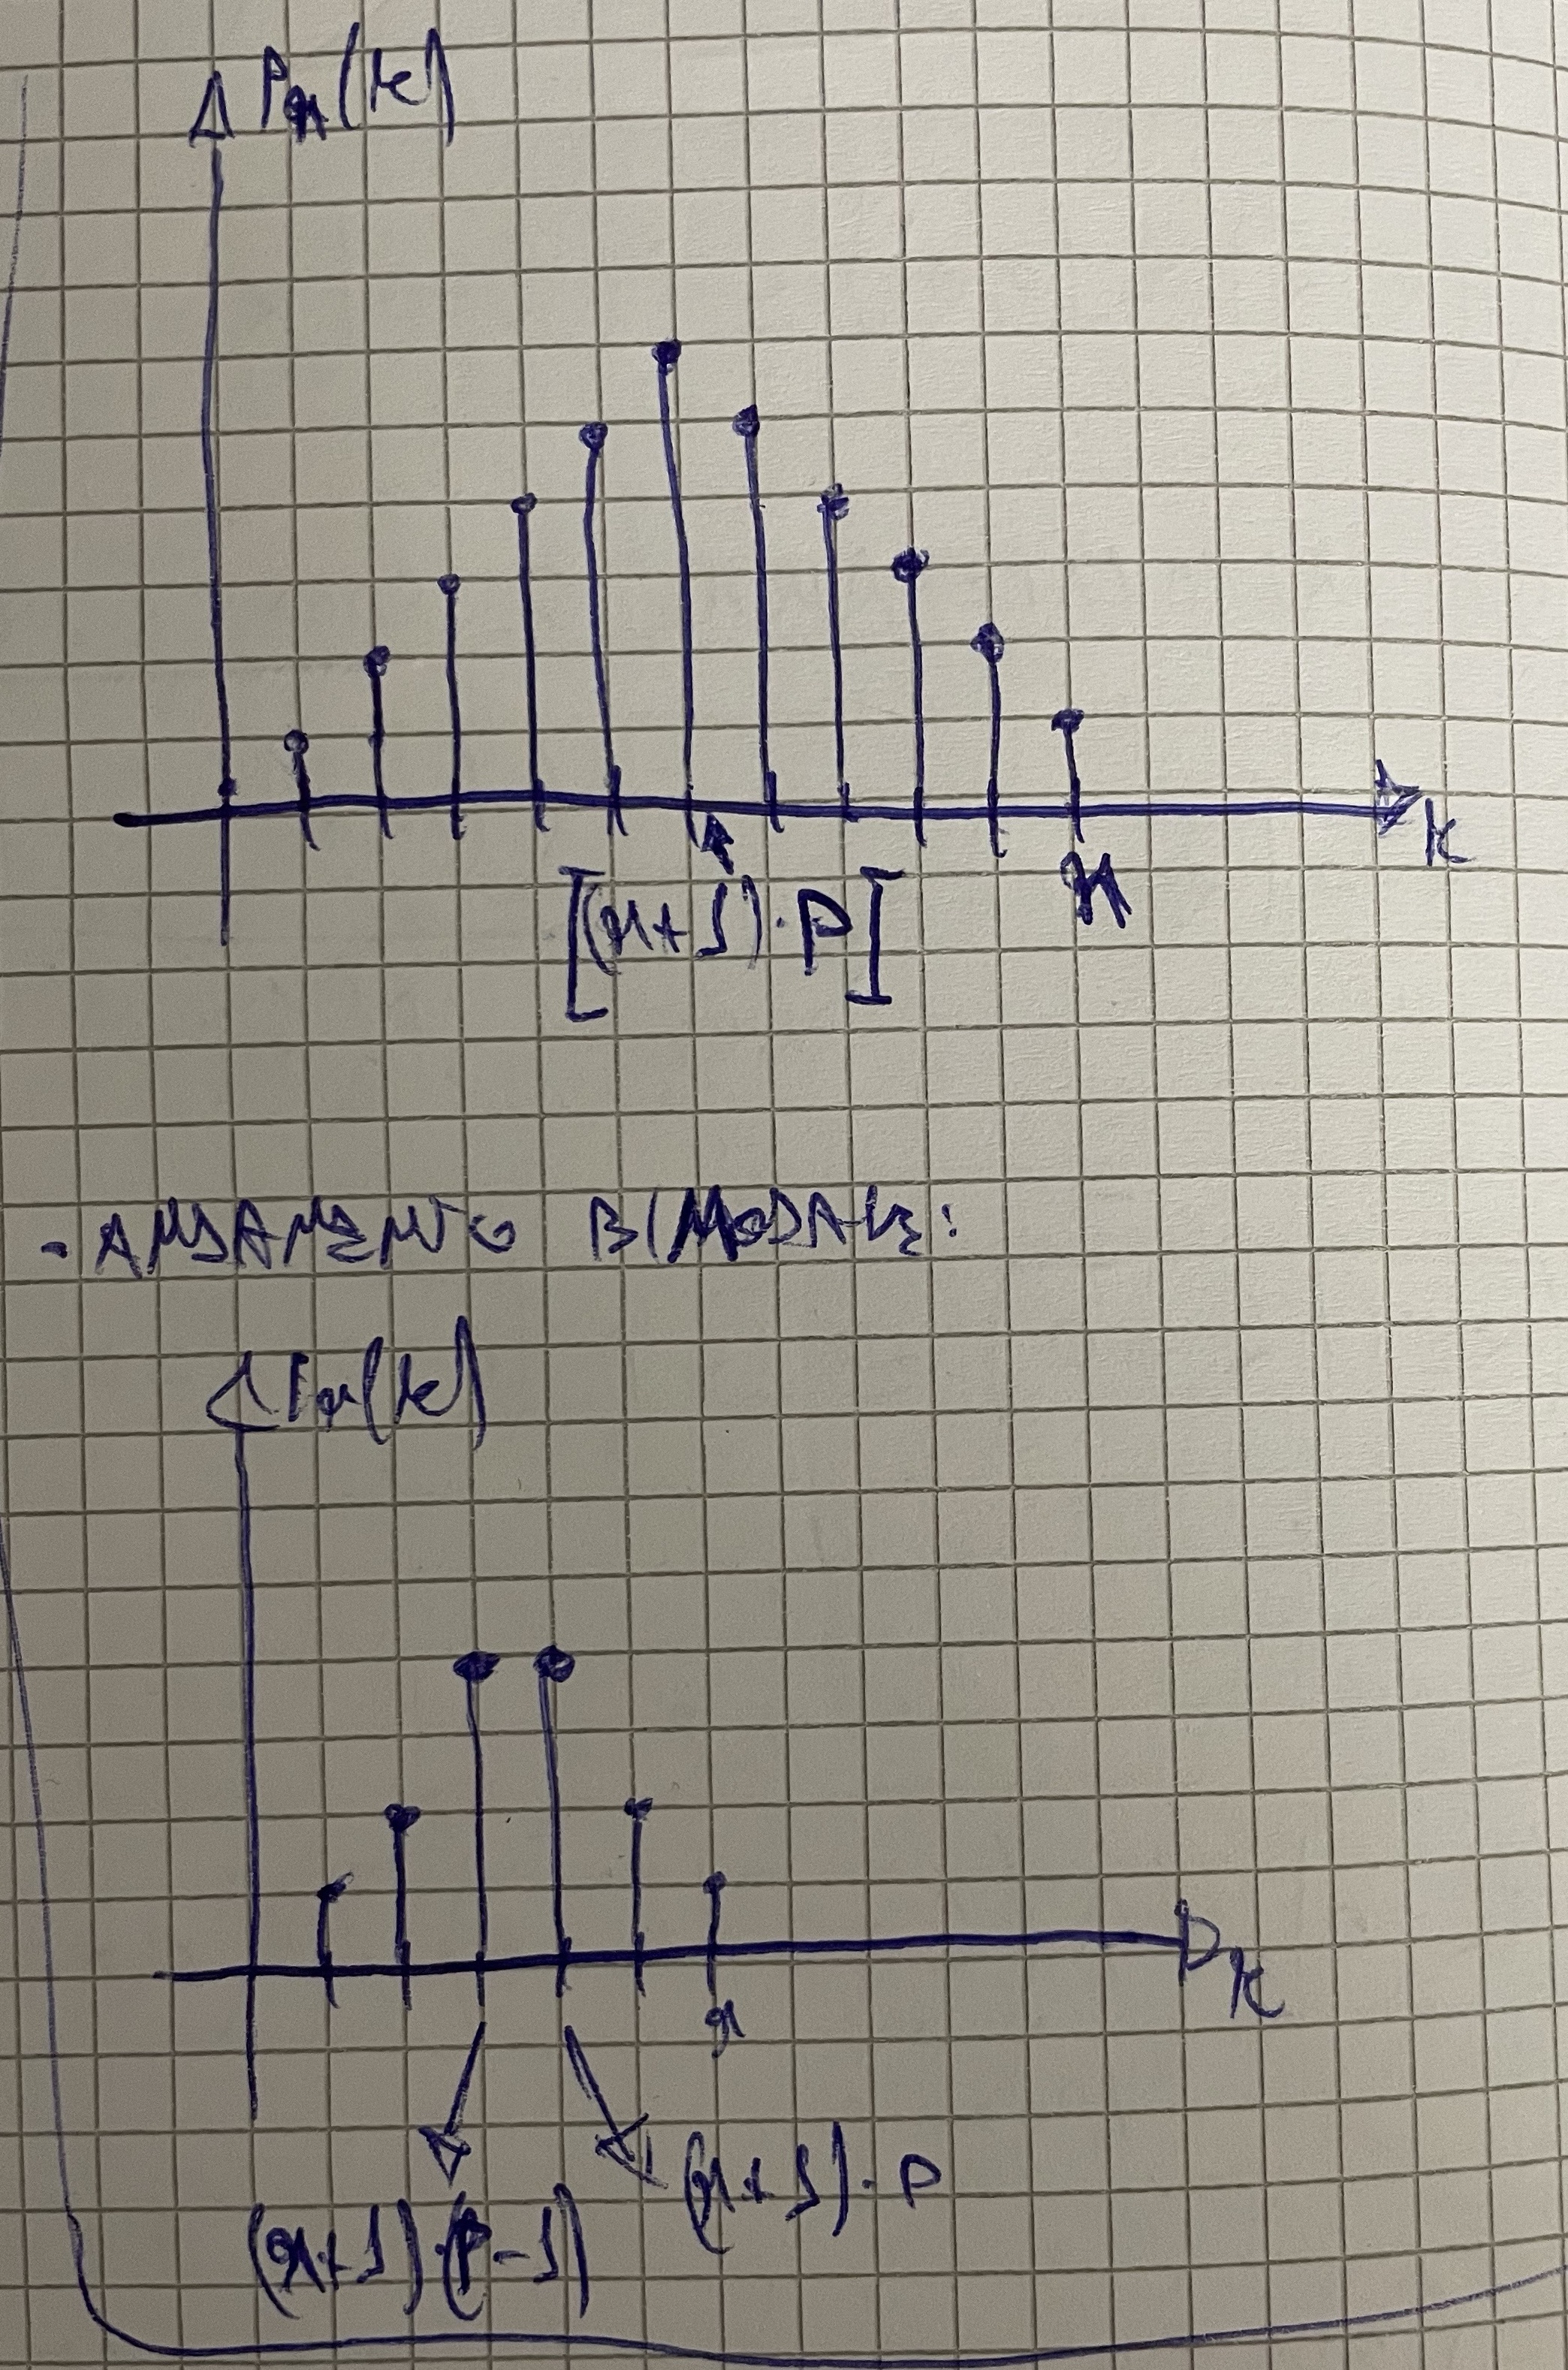
\includegraphics[scale=0.12]{images/25.ProvRip.jpeg}
\end{figure}

\subsubsection{\underline{Dimostrazione}}
Il rapporto fra la probabilità di avere $k-1$ successi su $n$ prove e la probabilità di avere $k$ successi su $n$ prove è uguale a 1. \\
$\frac{P_n(k-1)}{P_n(k)} = \frac{ \left( \begin{matrix} n \\ k-1 \end{matrix}\right) \cdot \cancel {p^{k-1}} \cdot q^{\cancel {n-k-1} } }
{ \left( \begin{matrix} n \\ k \end{matrix}\right) \cdot p^{\cancel k}\cdot \cancel {q^{n-k}} } =  \frac{ \frac{\cancel {n!}}{(k-1)! \cdot (n-k+1)!} \cdot q }
{ \frac{\cancel {n!}}{k! \cdot (n-k)!} \cdot p }$ \\
$=  \frac{ k! \cdot (n-k)! \cdot q }
{ (k-1)! \cdot (n-k+1)! \cdot p } = \frac{k \cdot q}{(n-k+1) \cdot p} < 1
\implies kq < np - kp + p $ \\
$\implies 
k \cdot (p+q) < np + p
\implies
k < (n+1) \cdot p$ \\
$\big[ k = (n+1) \cdot p\big]$ \\ \\
Se $(n+1) \cdot p$ è intero $\implies k = (n+1) \cdot p = \overline k$ \\ 
$\frac{P_n(\overline k-1)}{P_n(\overline k)} = \frac{\overline k q}{(n- \overline k +1) \cdot p} = \frac{(n+1) \cdot p \cdot q}{(n-np \underset{q}{\underbrace{-p-1}} ) \cdot p}
= \frac{npq + pq}{(nq + q)  \cdot p} = \frac{npq + pq}{npq +pq} = 1$ \\
\hspace*{0pt}\hfill $\square$
\newpage
\subsubsection{\underline{Esempio 1}} 
\begin{figure}[ht]
\centering
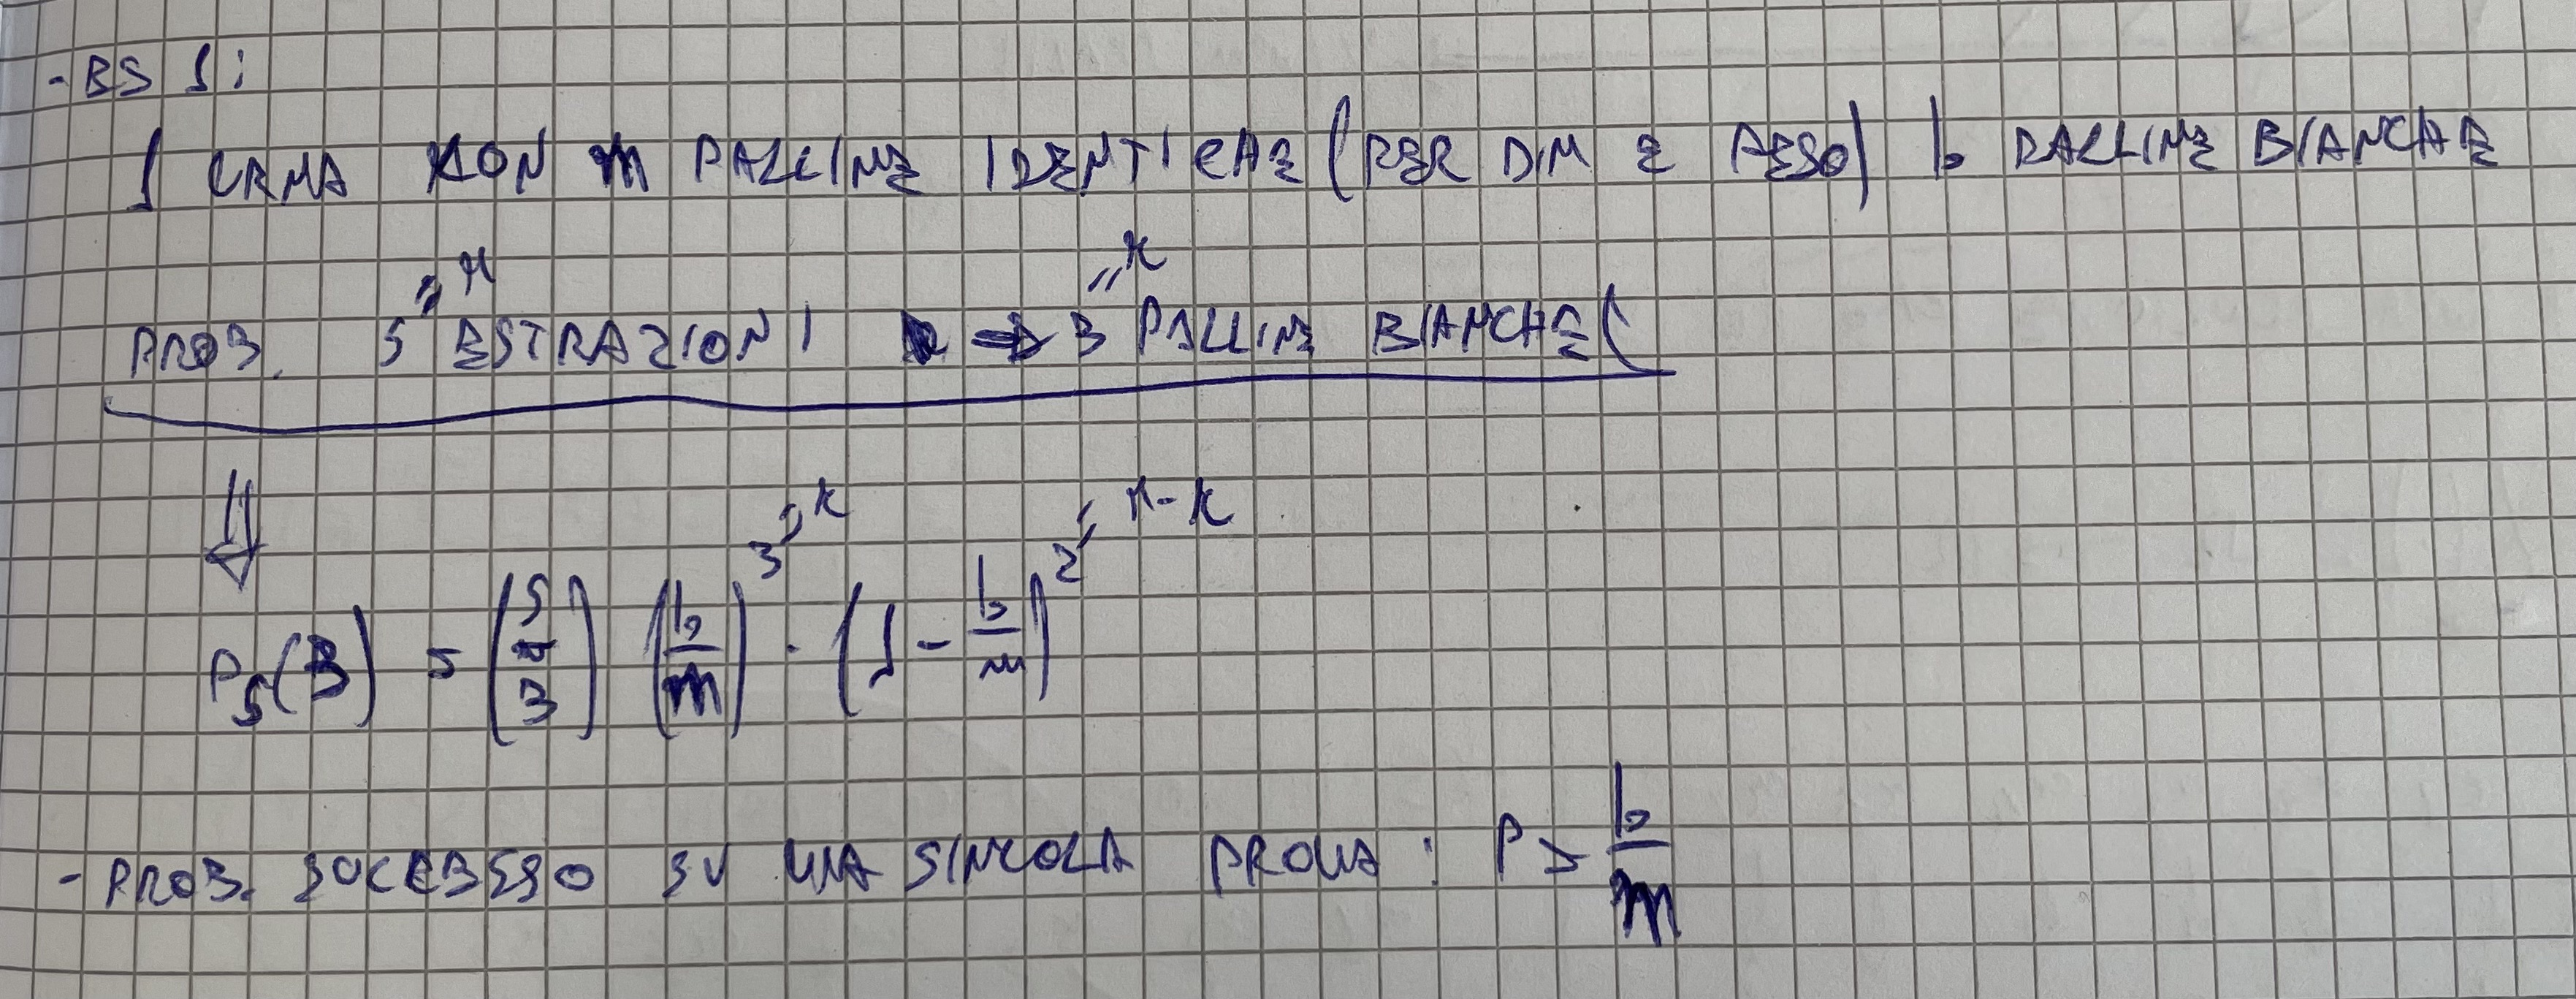
\includegraphics[scale=0.12]{ese/7.jpeg}
\end{figure}
\subsubsection{\underline{Esempio 2}} 
\begin{figure}[ht]
\centering
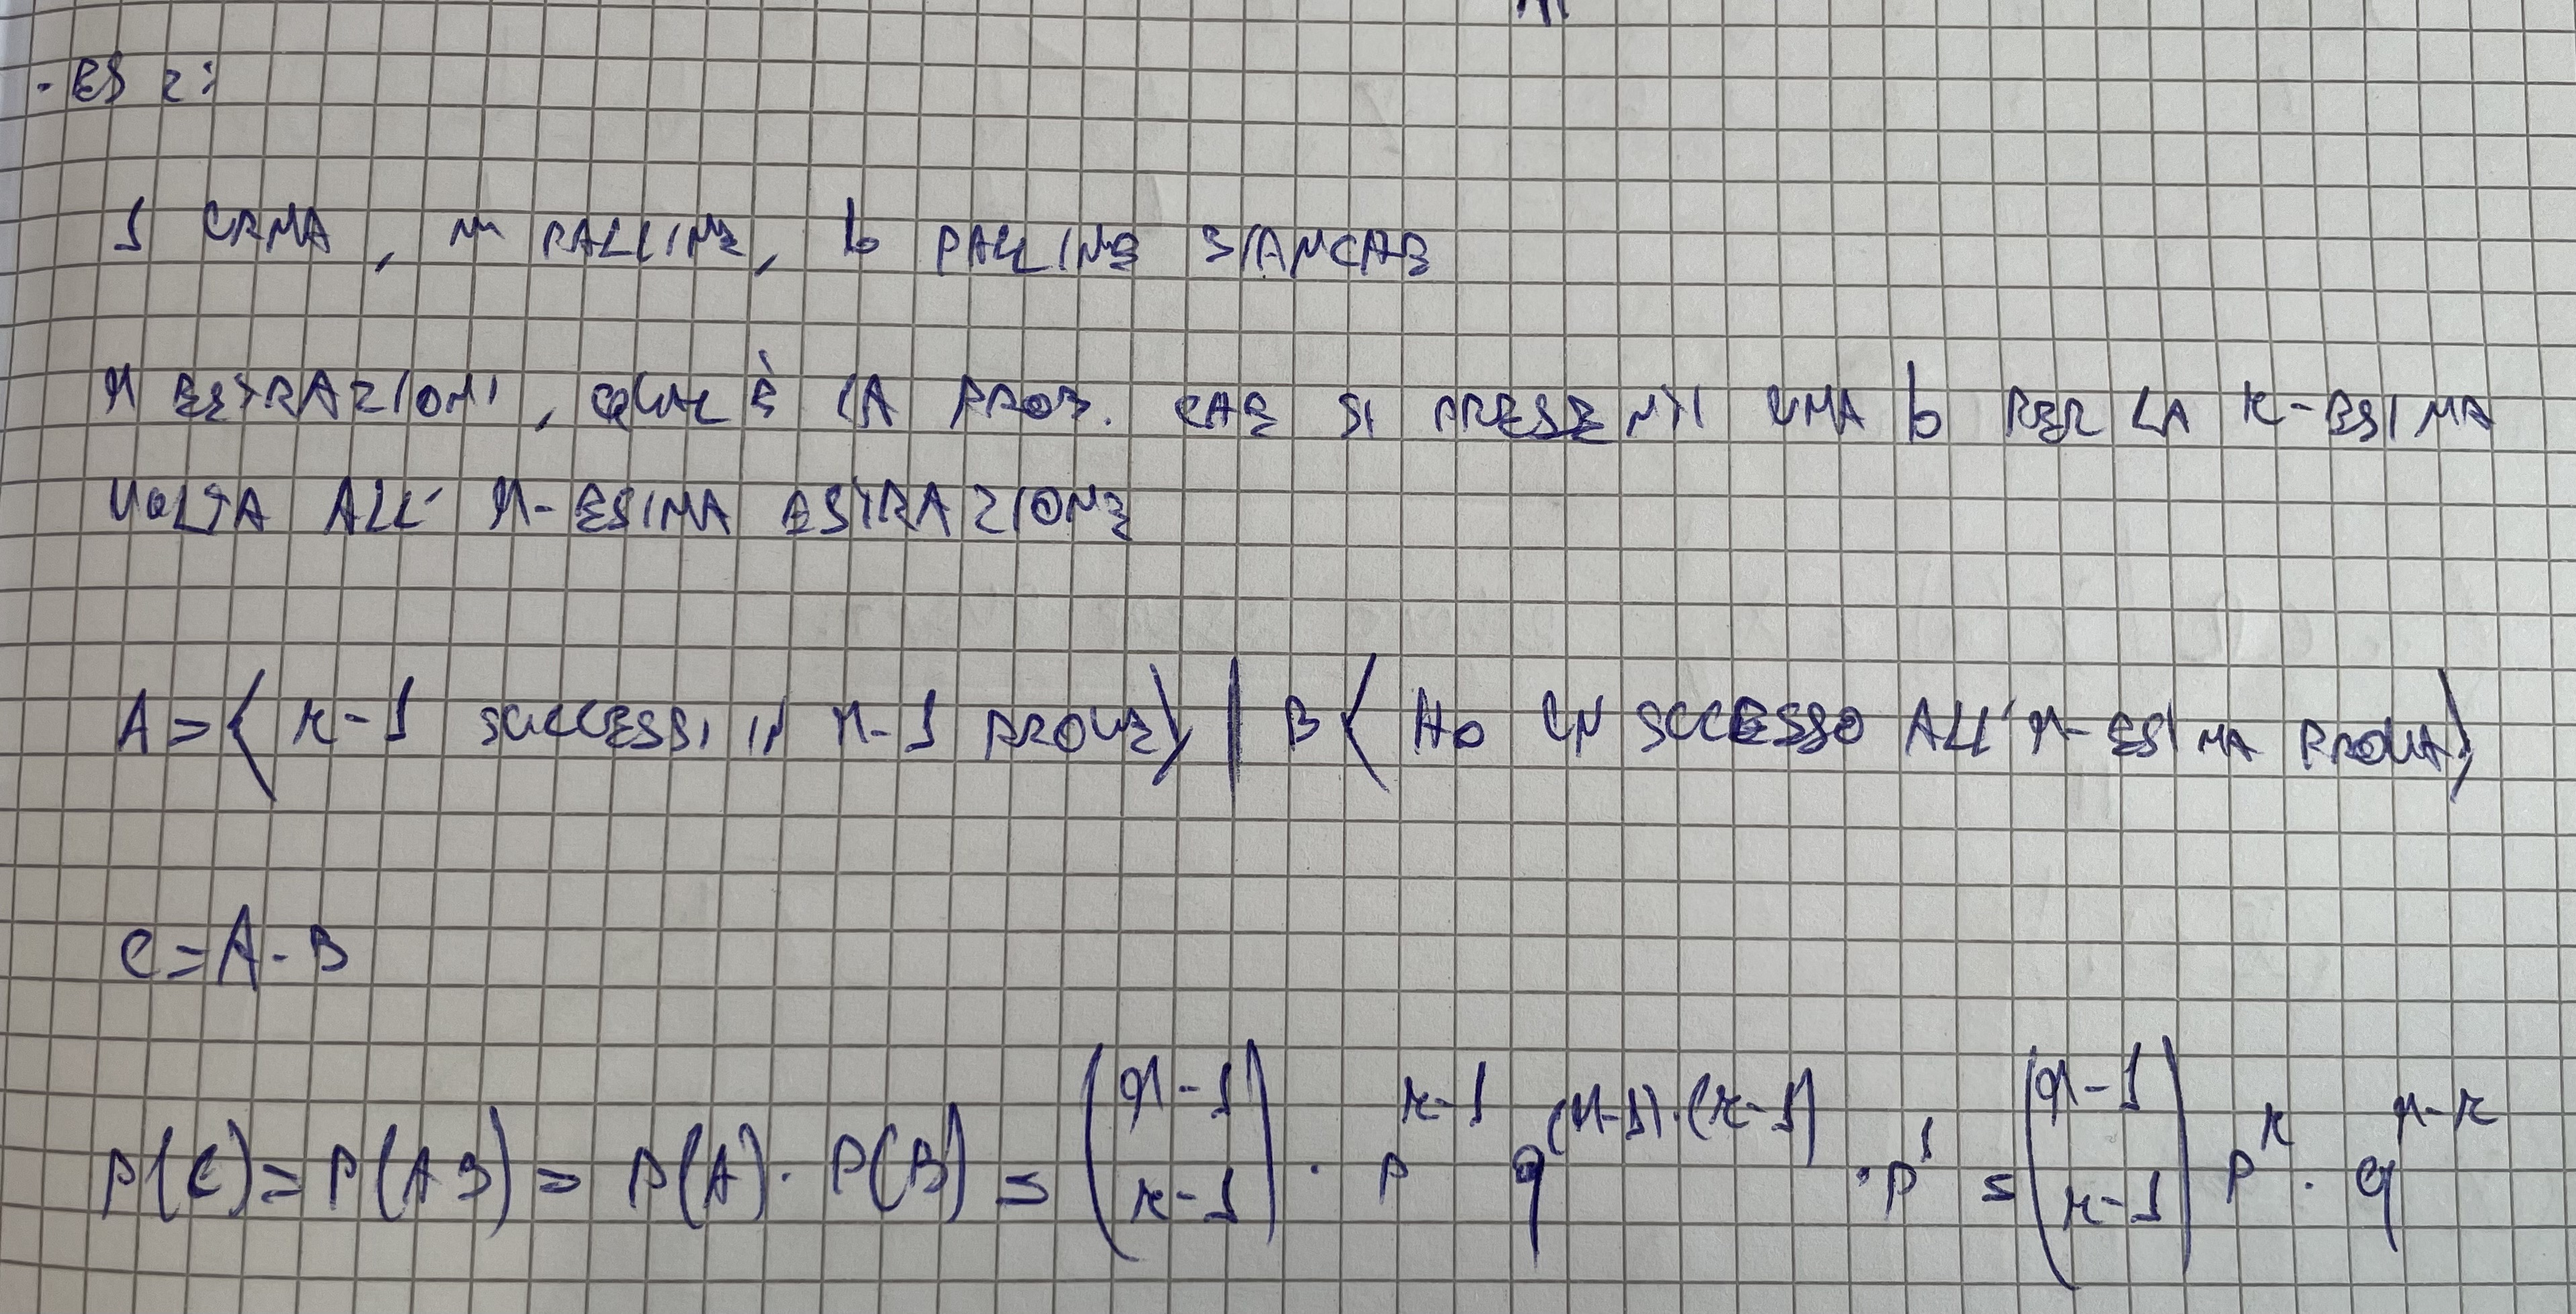
\includegraphics[scale=0.12]{ese/8.jpeg}
\end{figure}
\newpage
\subsection{Esempi sul capitolo}
\subsubsection{\underline{Esempio 1}}
\begin{figure}[ht]
\centering
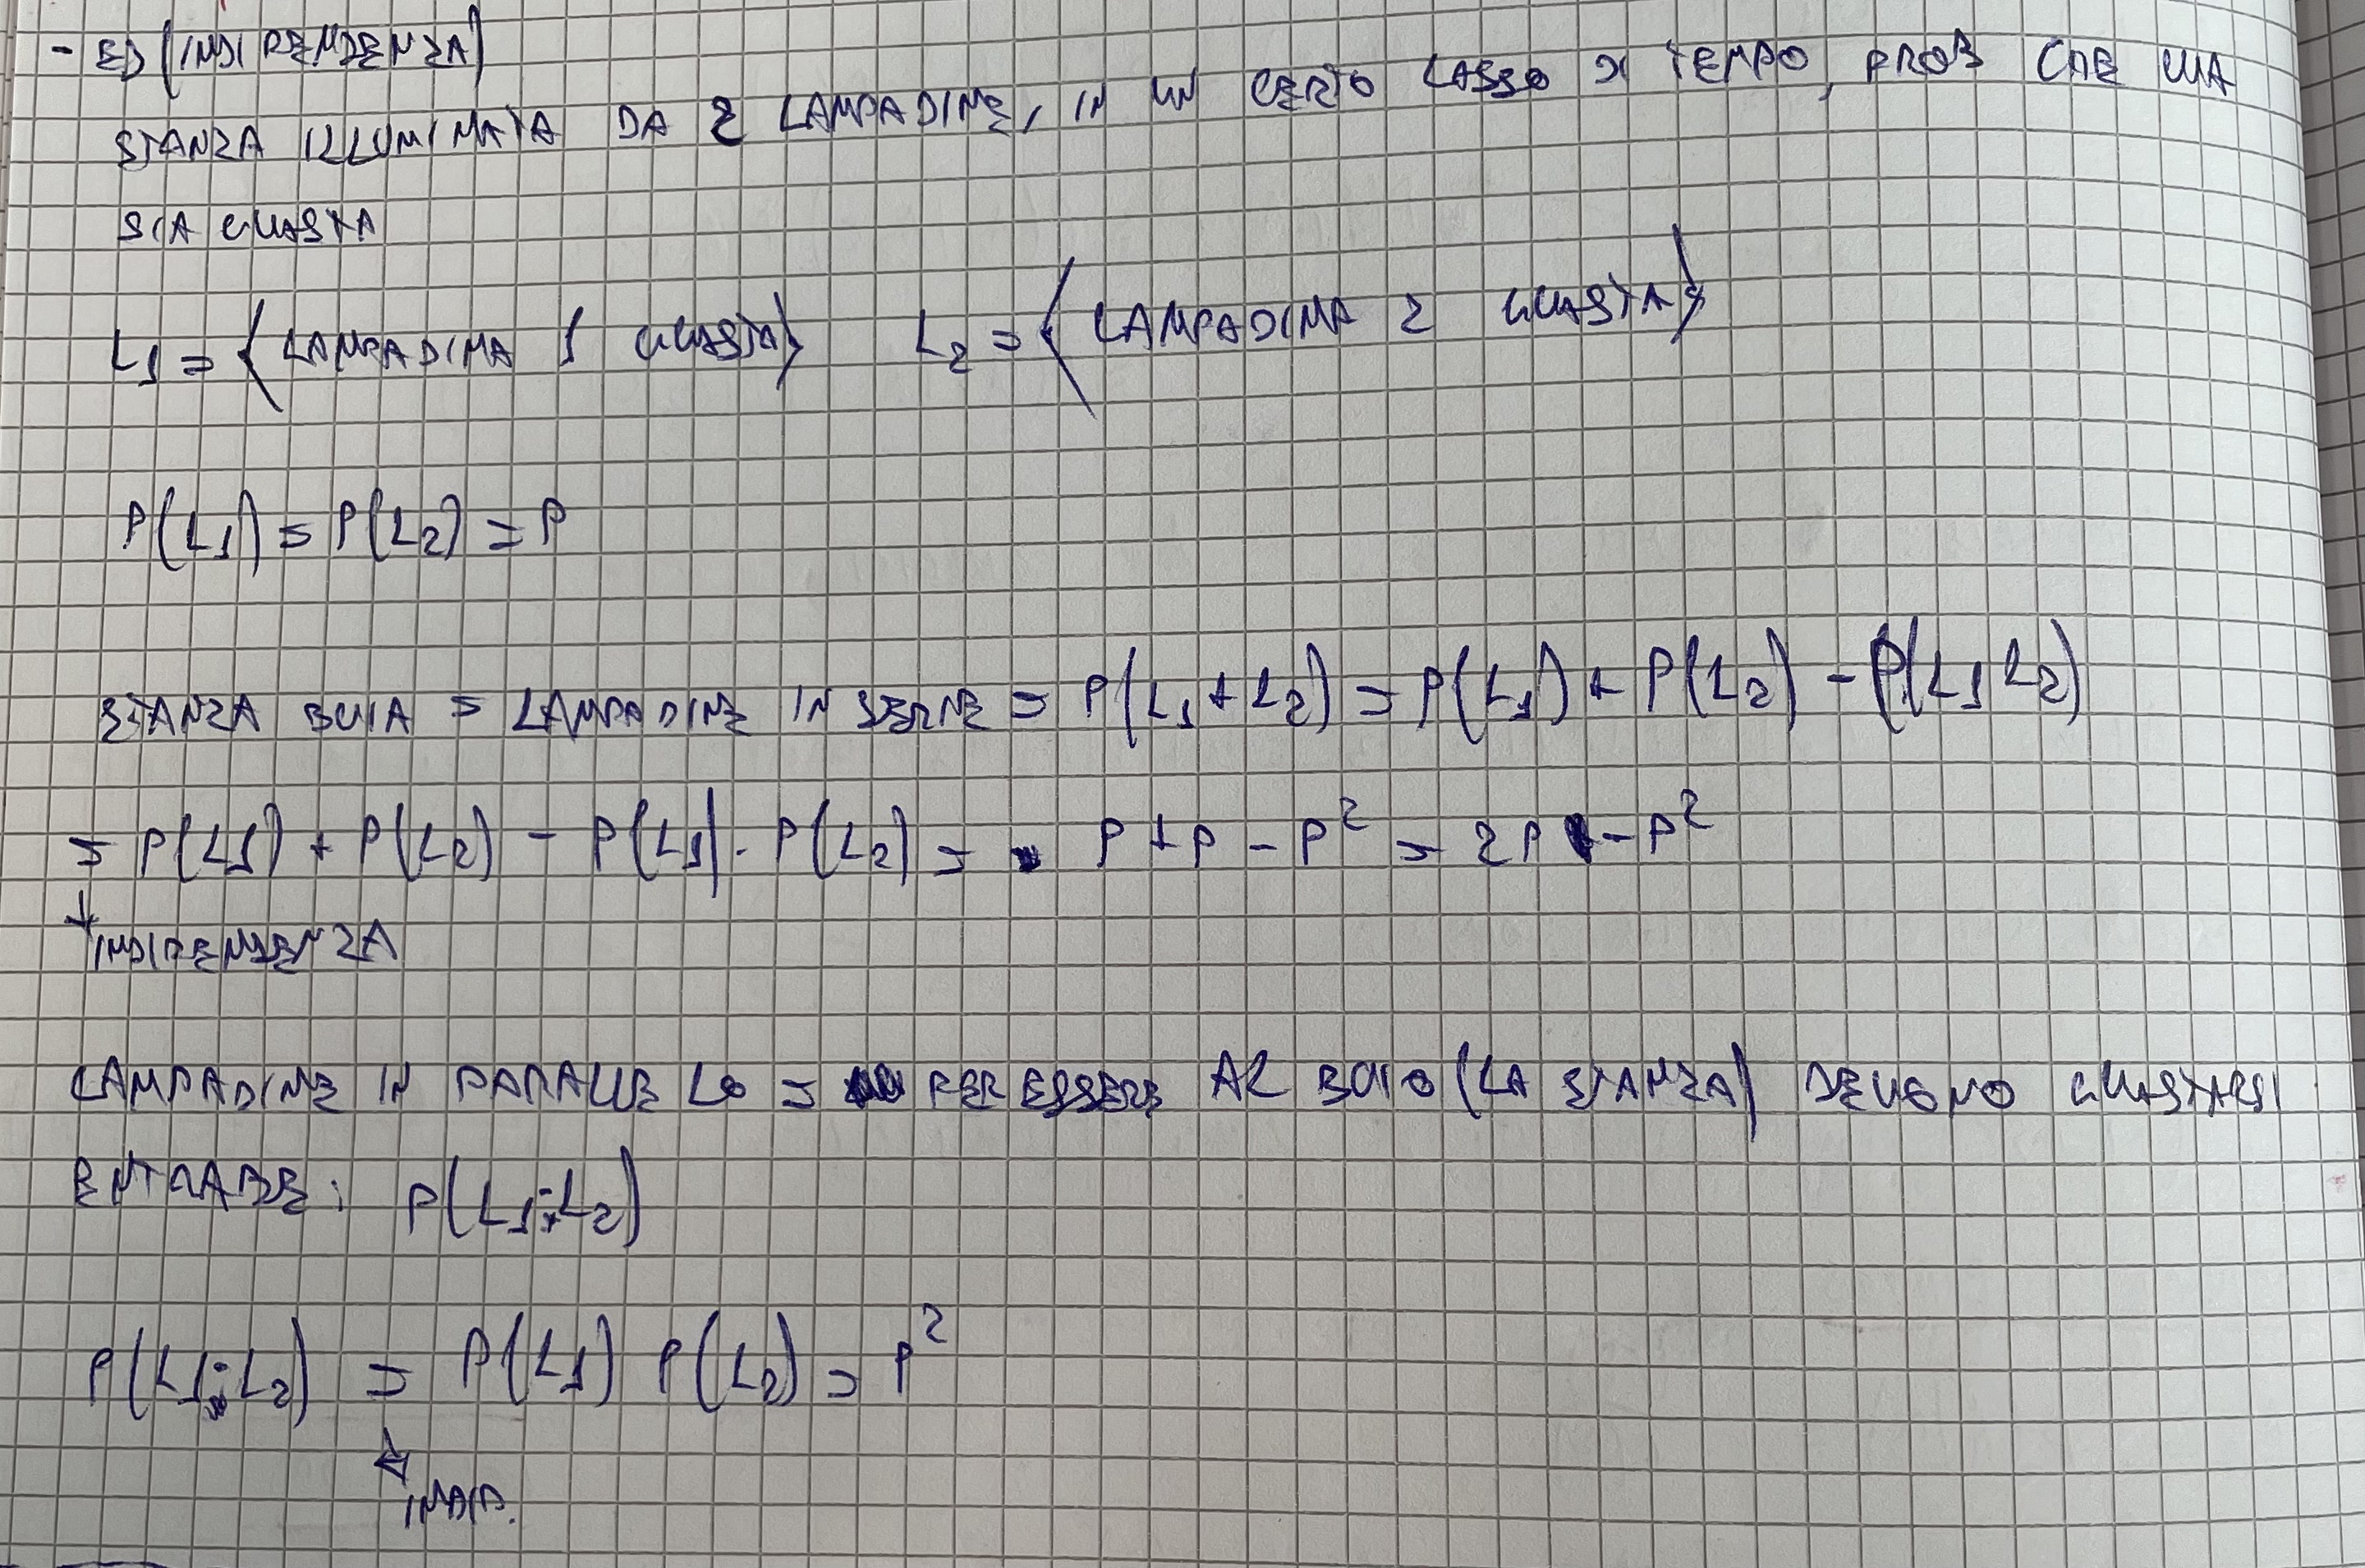
\includegraphics[scale=0.12]{ese/9.jpeg}
\end{figure}
\subsubsection{\underline{Esempio 2}}
\begin{figure}[ht]
\centering
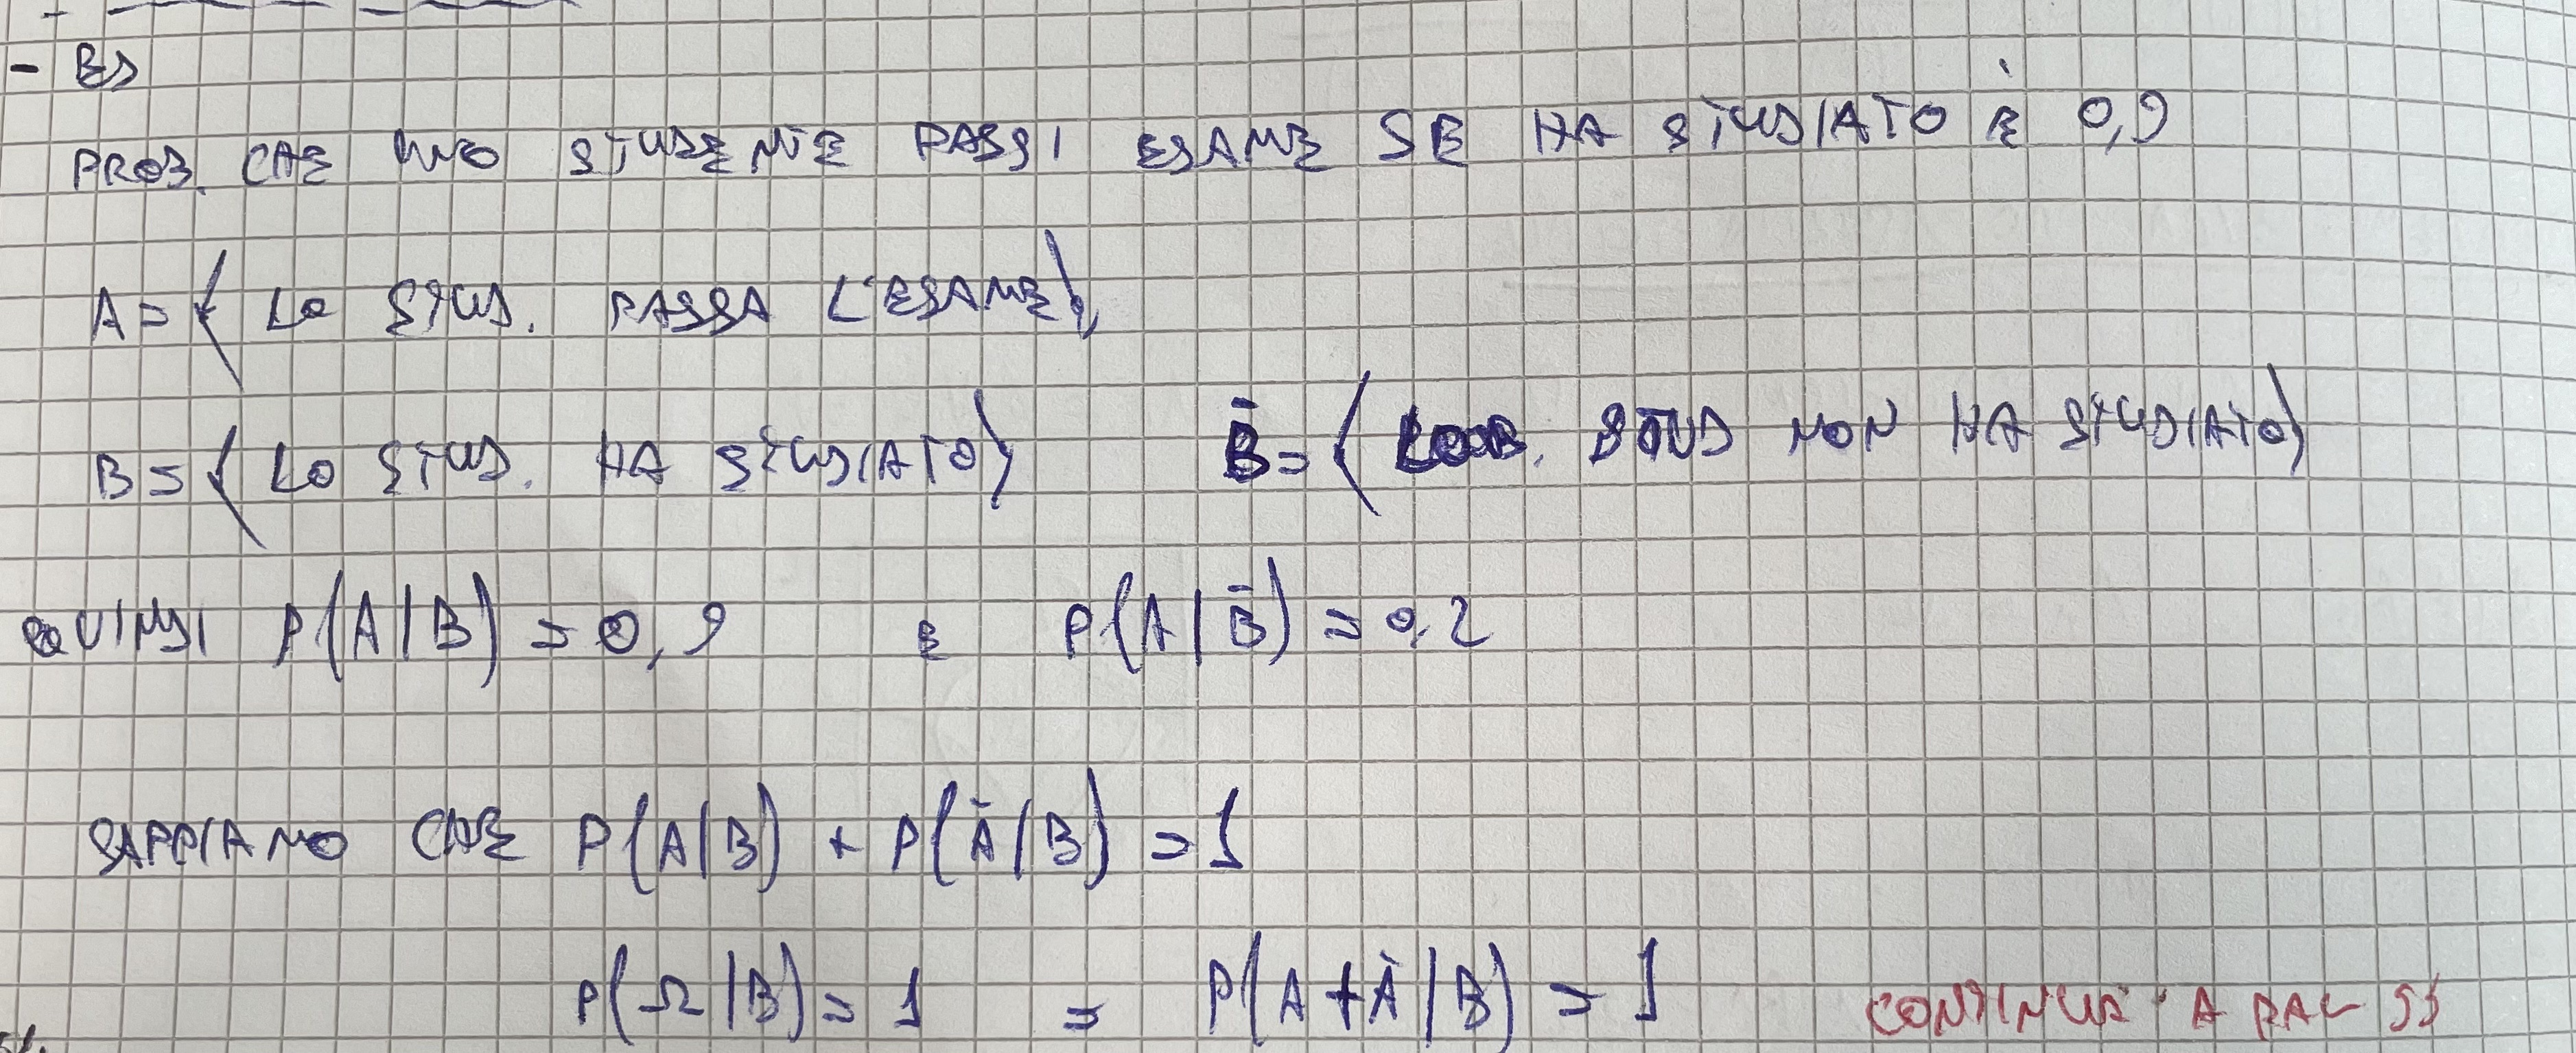
\includegraphics[scale=0.12]{ese/10.jpeg}
\end{figure}
\begin{figure}[ht]
\centering
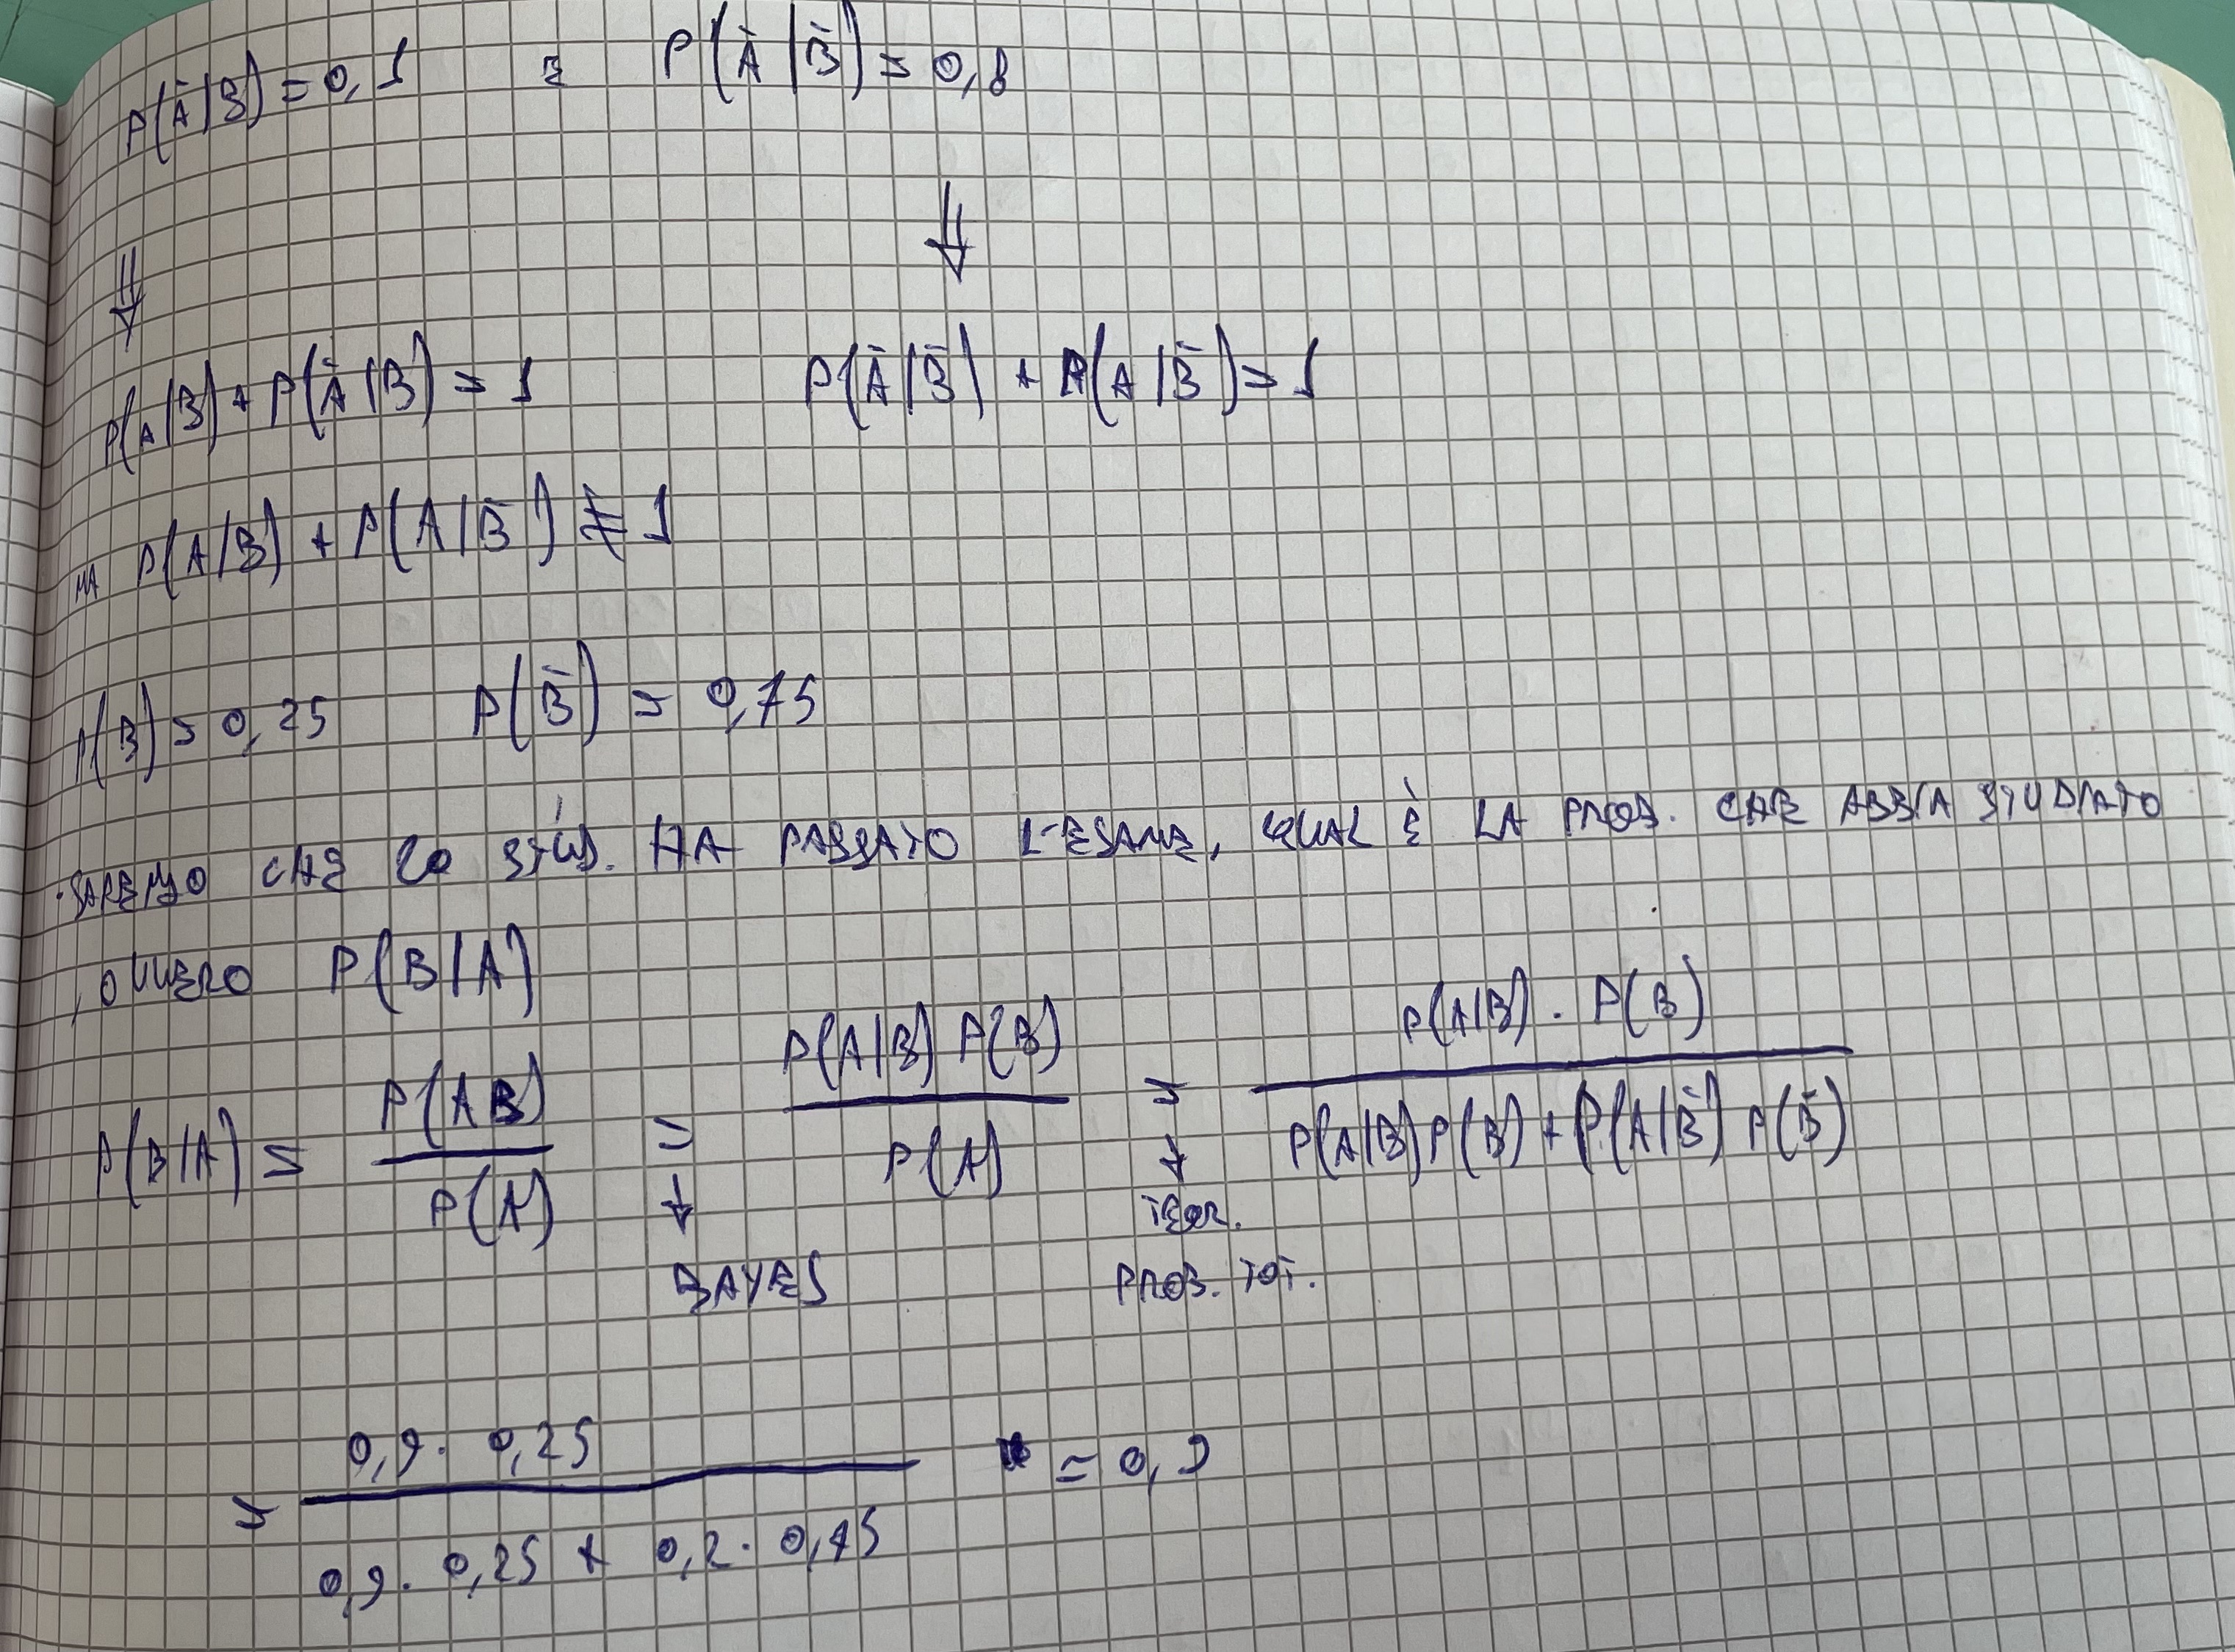
\includegraphics[scale=0.12]{ese/10a.jpeg}
\end{figure}
\newpage
\subsubsection{\underline{Esempio 3}}
\begin{figure}[ht]
\centering
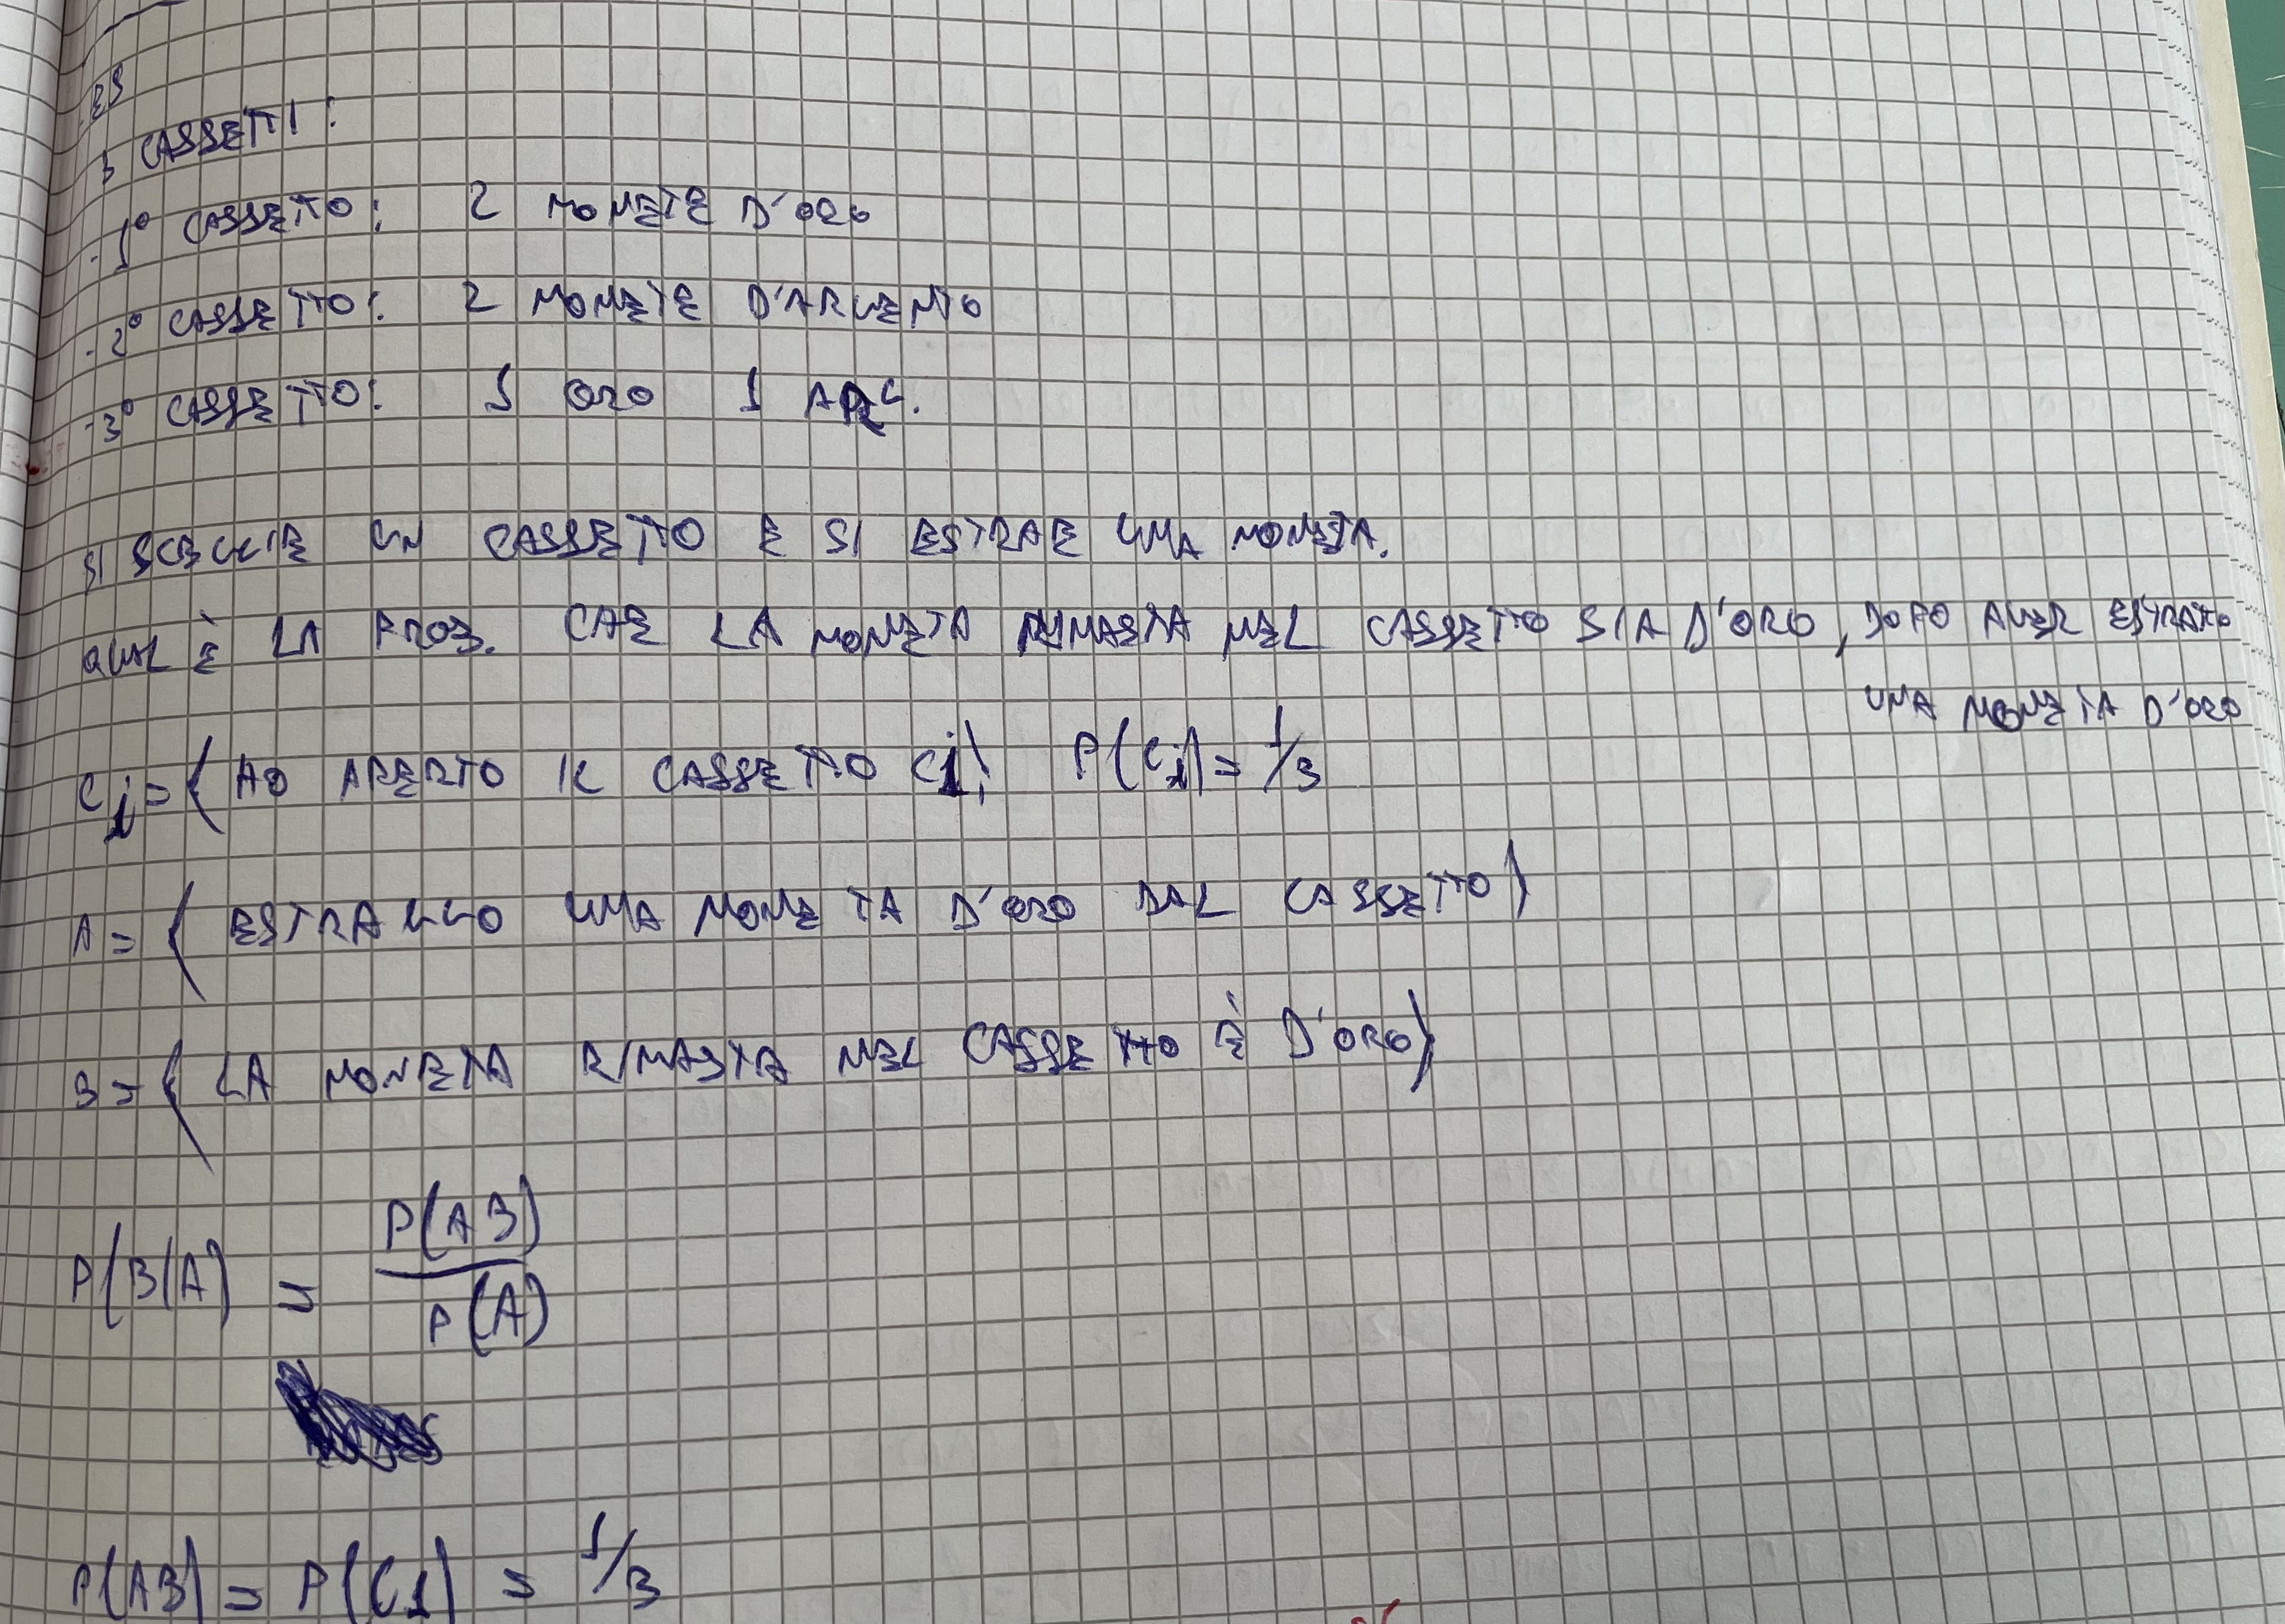
\includegraphics[scale=0.10]{ese/11.jpeg}
\end{figure}
\begin{figure}[ht]
\centering
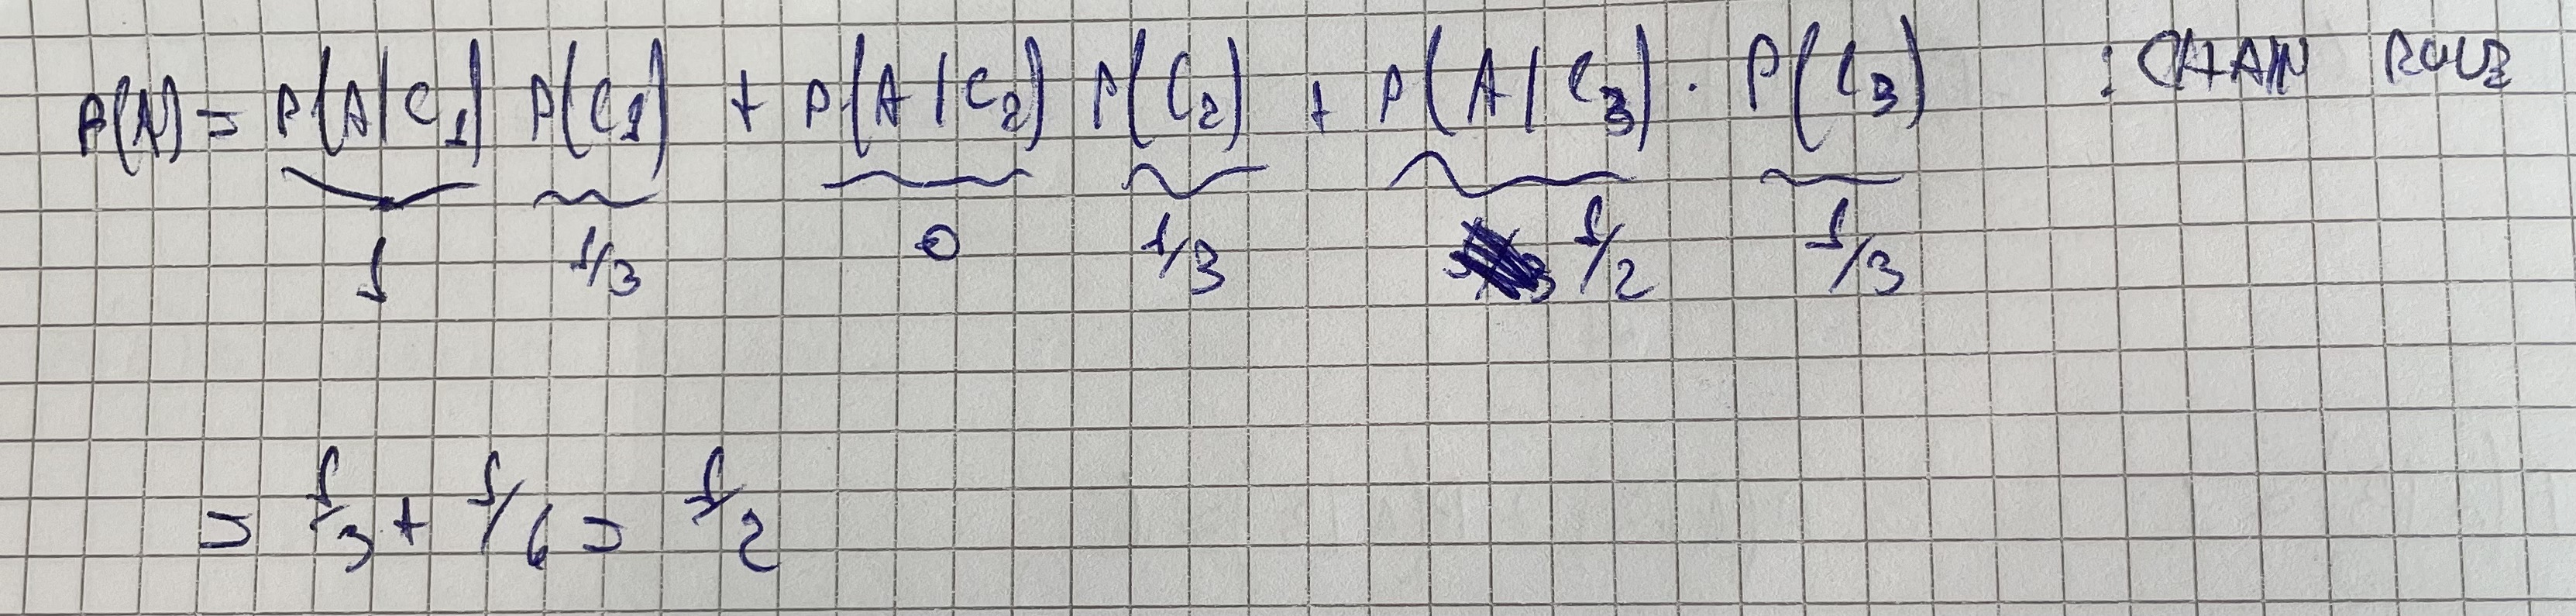
\includegraphics[scale=0.10]{ese/11a.jpeg}
\end{figure}
\newpage
\subsubsection{\underline{Esempio 4}}
\begin{figure}[ht]
\centering
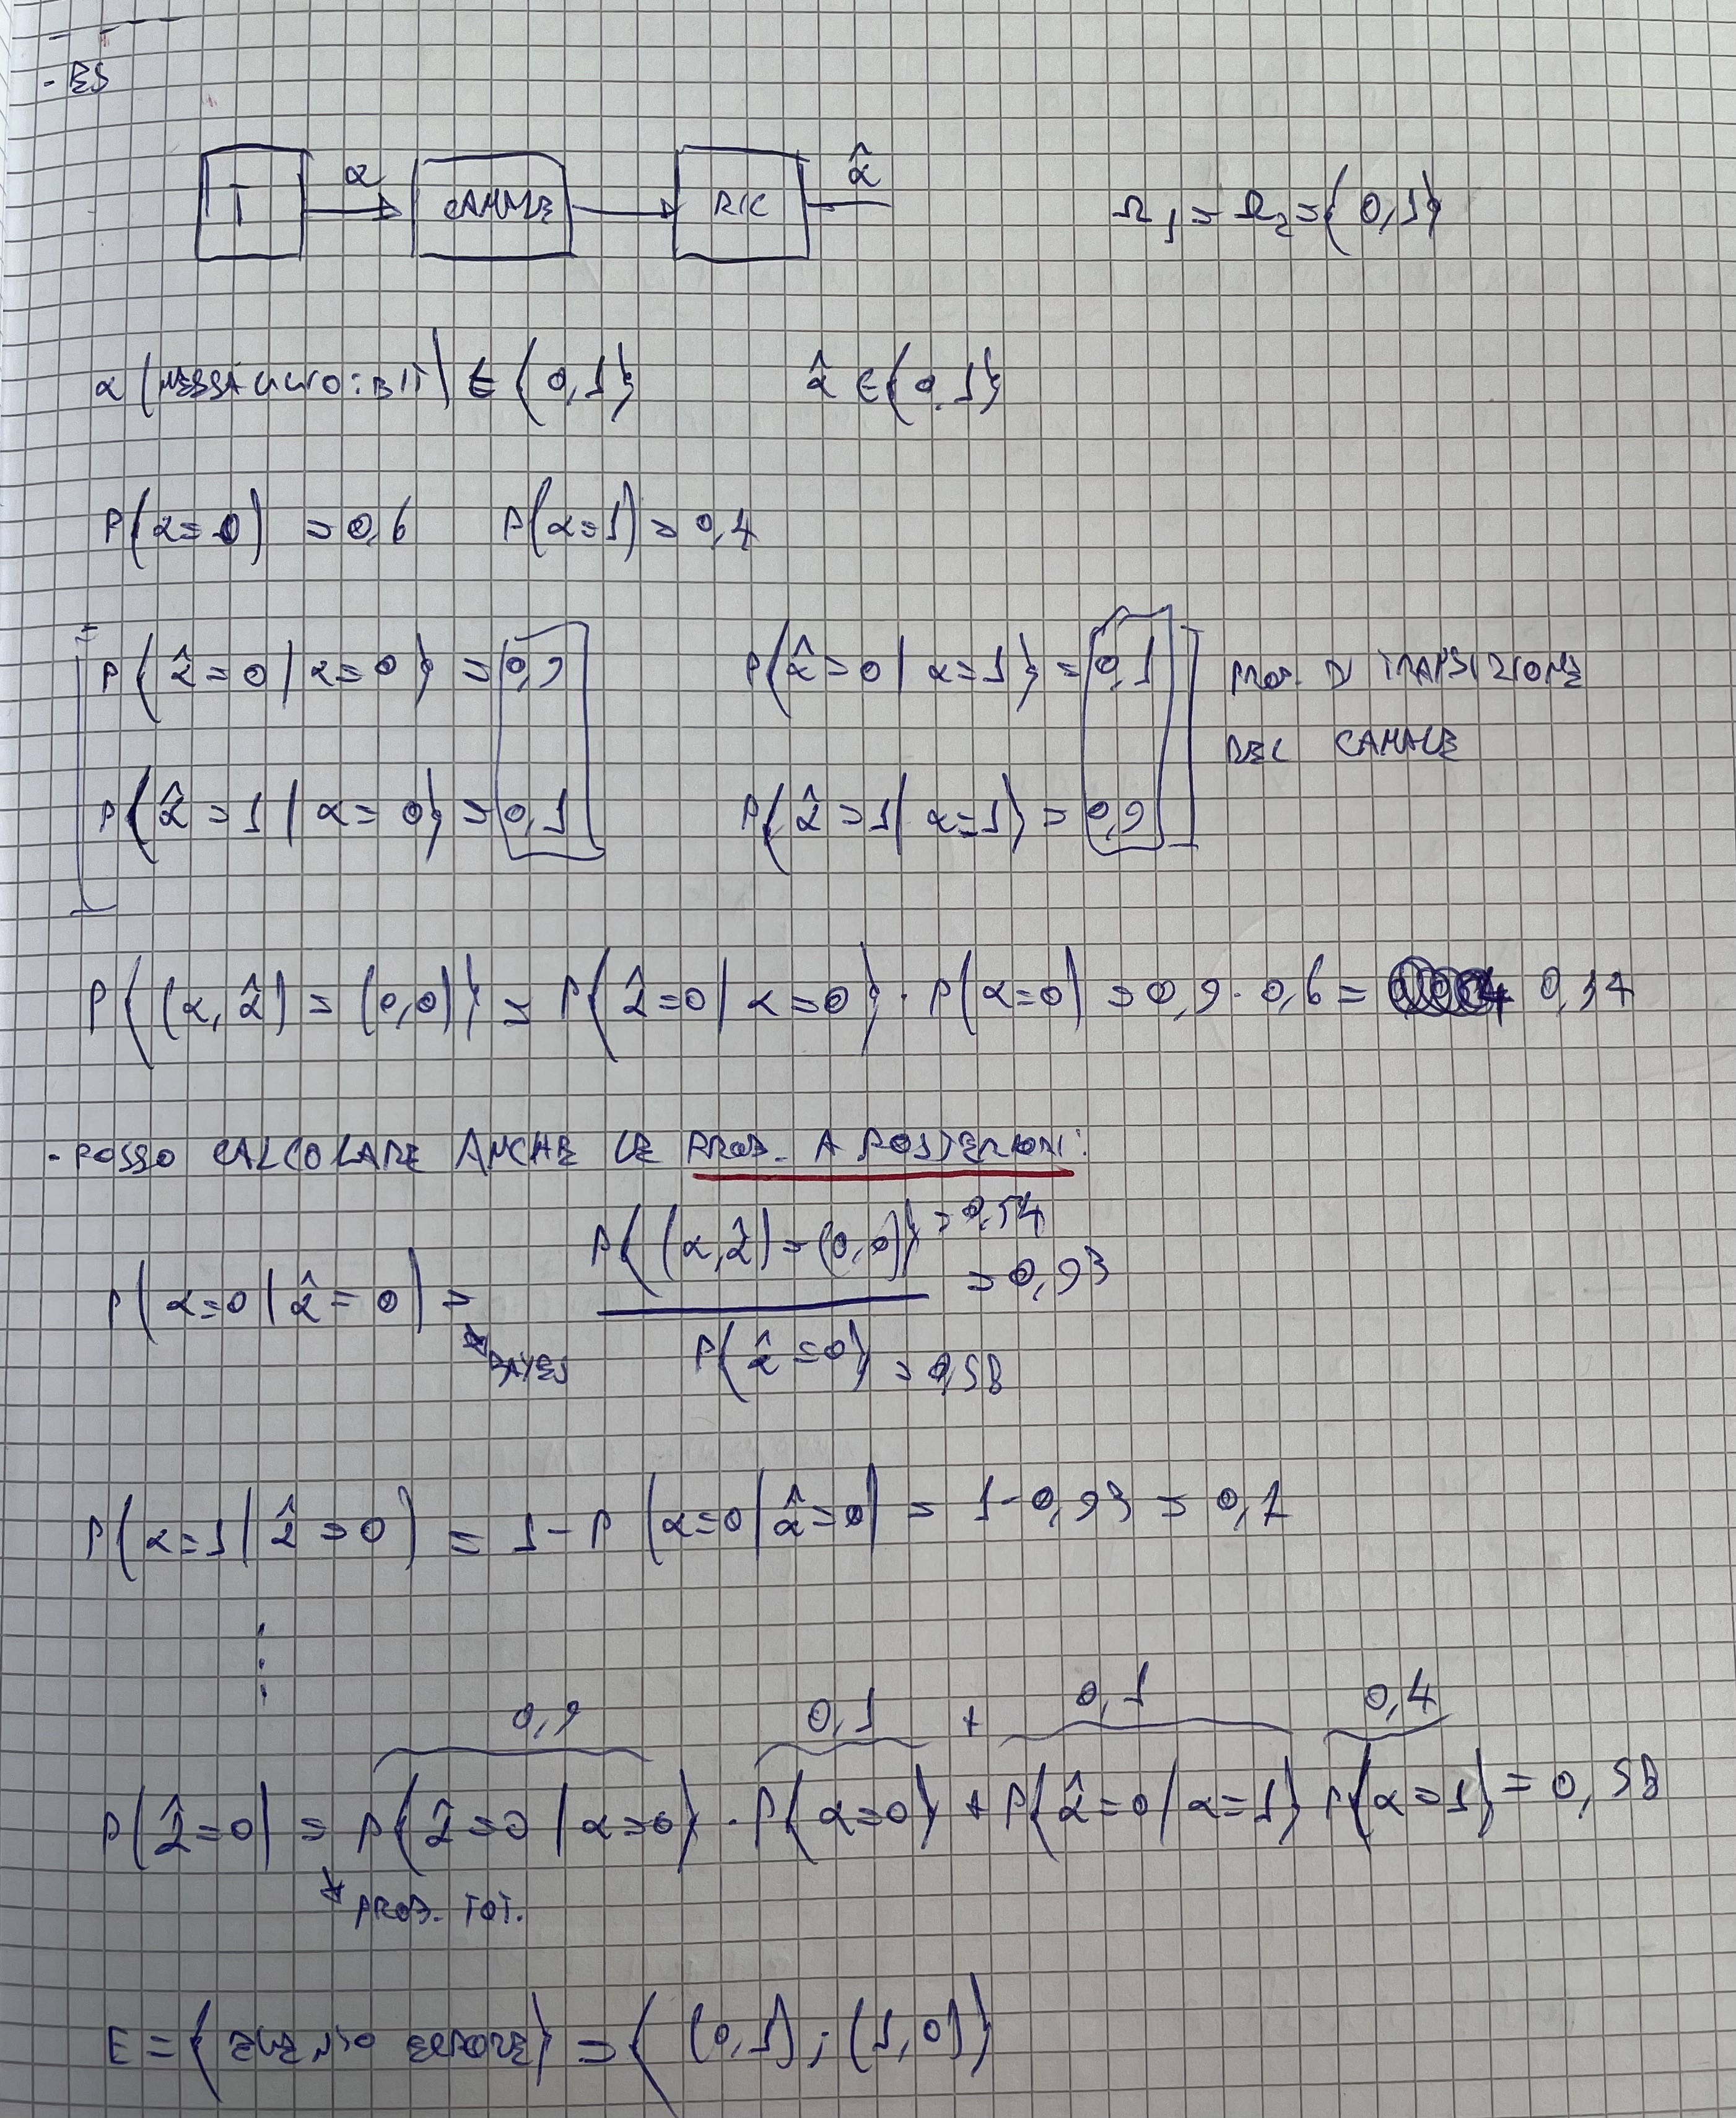
\includegraphics[scale=0.12]{ese/12.jpeg}
\end{figure}

\section{Variabili Aleatorie}
\subsection{Introduzione}
\begin{tabular}{|p{13cm}}
Una variabile aleatoria non è altro che una variabile definita associando ad ogni risultato di un esperimento un numero reale o complesso.
\end{tabular}
\newpage
\begin{figure}[ht]
\centering
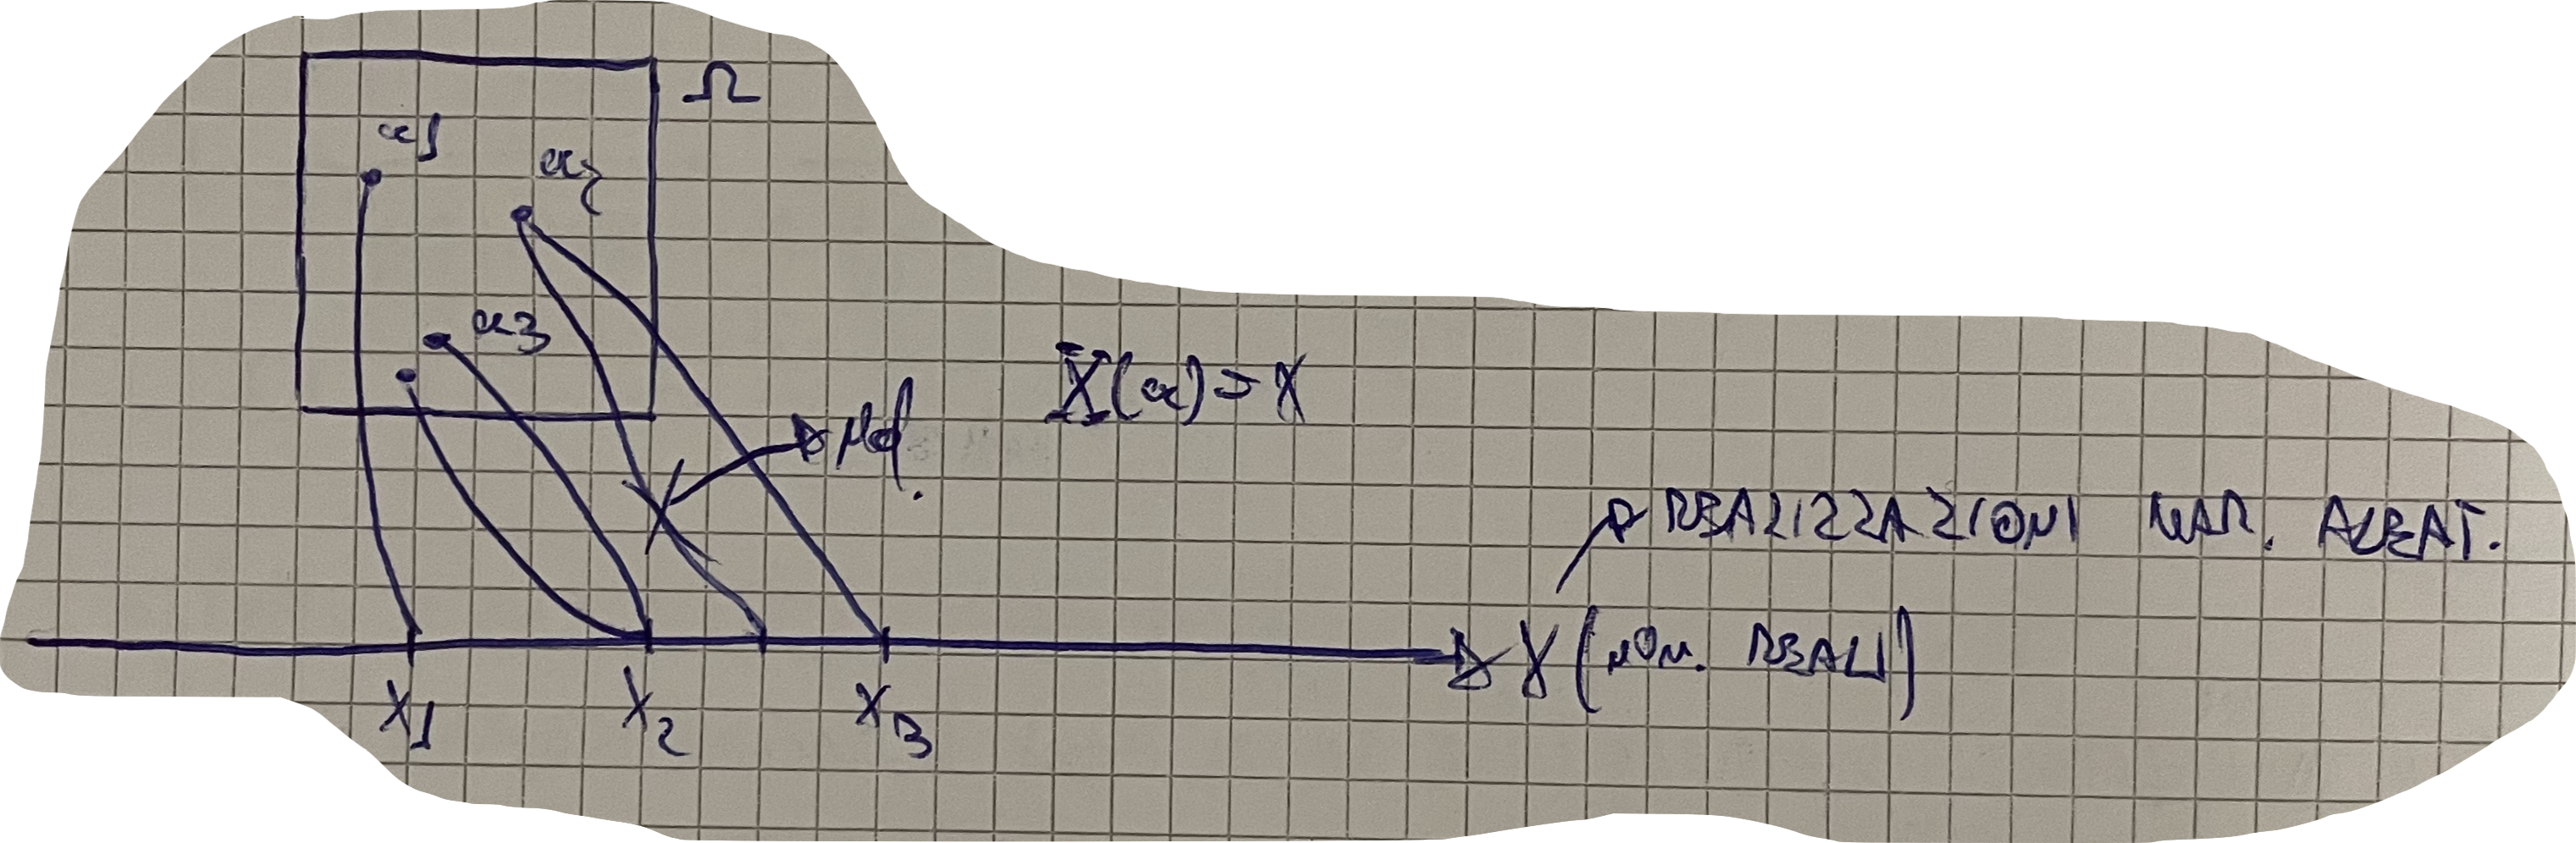
\includegraphics[scale=0.12]{images/26.V.A.png}
\end{figure} 
\subsubsection{\underline{Proprietà}}
\begin{enumerate}
    \item La variabile aleatoria $X(a)$ è una funzione che va da $\Omega$ e $\mathbb{R}$, ovvero: $X(\cdot) : \Omega \rightarrow \mathbb{R}$
    \subsubsection{\underline{Esempio1(Facce dado)}}
    Ad ogni risultato di un esperimento $\left( a_i \right)$ associamo un valore della V.A. $X$: 
    \[\begin{matrix}
    & a_1 & a_2 & a_3 & a_4 & a_5 & a_6 \\
    X& \downarrow & \downarrow & \downarrow & \downarrow & \downarrow & \downarrow \\
    & 1 & 2 & 3 & 4 & 5 & 6
    \end{matrix}\]
    \subsubsection{\underline{Esempio2(Divisione fra facce pari e dispari)}}
    Ad ogni risultato di un esperimento $\left( a_i \right)$ associamo un valore della V.A. $Y$, se il risultato è una faccia pari ci assoceremo il numero $1$, se invece è dispari, ci assoceremo il numero $0$:
    \[\begin{matrix}
    & a_1 & a_2 & a_3 & a_4 & a_5 & a_6 \\
    Y & \downarrow & \downarrow & \downarrow & \downarrow & \downarrow & \downarrow \\
    & 0 & 1 & 0 & 1 & 0 & 1
    \end{matrix}\]
    \item Tutti gli insiemi del tipo $\Big\{ a \in \Omega \big| X(a) \leq x_i \Big\} = \big\{X \leq x_i \big\}$ devono essere degli eventi.
    \item $P\{X = \pm \infty \} = 0$
\end{enumerate}
\begin{tabular}{|p{13cm}}
Nelle variabili aleatorie, gli elementi che prima componevano un sistema di probabilità non sono uguali, ma si devono adattare al “mondo” delle V.A.  nel seguente modo: \\ \\
\[\begin{matrix}
\#\text{Sistema di probabilità: } & \Omega & \mathcal{I} & P\\
 & \downarrow & \downarrow & \downarrow\\
\#\text{Sistema di probabilità con l'utilizzo di V.A.: } & \mathbb{R} & \big\{X \leq x_i\big\} & P
\end{matrix}\]
\end{tabular}

\subsection{CDF: Funzione di Distribuzione (o Cumulatrice)}
\begin{tabular}{|p{13cm}}
La CDF o Cumulative Distribution Function viene definita come:
\[F_X(x) = P\big\{ X \leq x_i \big\} \;\big|\; \lim_{x \to -\infty} F_X(x) = 0  \;\big|\; \big[ \{a \in \Omega | X(a) \leq x\}\big]\]
\end{tabular}
\subsubsection{\underline{Proprietà}}
\begin{enumerate}
    \item $0 \leq F_X(x) \leq 1$
    \item $P \big\{ x_1 \leq X \leq x_2 \big\} = F_X(x_2) - F_X(x_1)$
    \newpage
    \paragraph{\underline{Dimostrazione}}
    $P \big\{ x_1 \leq X \leq x_2 \big\} \implies {\color{green}\underline{P \big\{ X \leq x_2 \big\}}} = \underset {\text{2 eventi disgiunti}}{\underline{P \big\{X \leq x_1 \big\}} + P \big\{ x_1 < X \leq x_2 \big\}}$ ~\\
    \begin{figure}[ht]
    \centering
    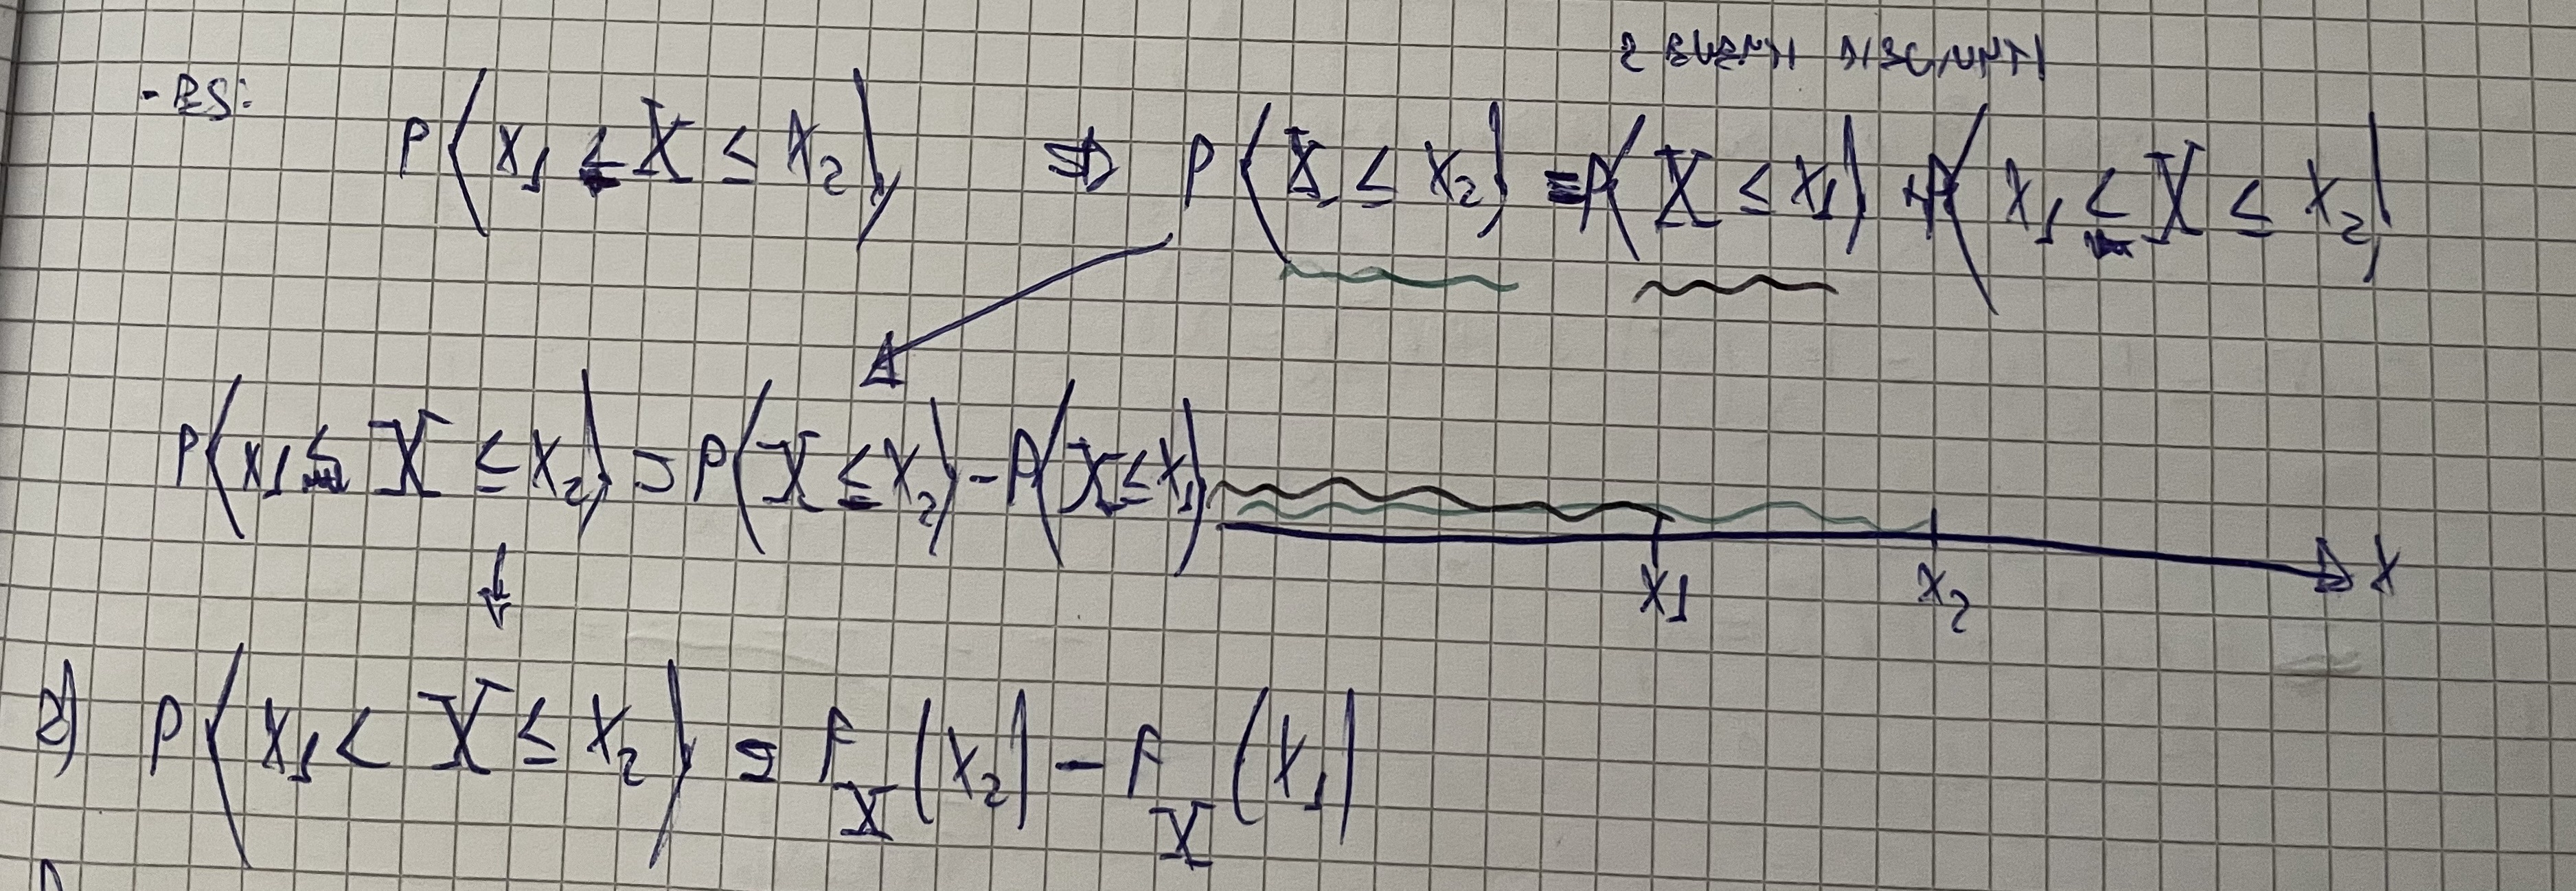
\includegraphics[scale=0.12]{images/27.prop2CDF.jpeg}
    \end{figure} ~\\
    $\implies P\big\{ x_1 < X \leq x_2 \big\} = P \big\{X \leq x_2\big\} - P \big\{ X \leq x_1\big\}$ \\
    $\implies P \big\{ x_1 \leq X \leq x_2 \big\} = F_X(x_2) - F_X(x_1)$ \\
    \hspace*{0pt}\hfill $\square$
    \item La CDF è una funzione monotona non decrescente, ovvero: $x_1 \leq x_2 \implies F_X(x_1) \leq F_X(x_2)$
    \item $\lim_{x \to -\infty} F_X(x) = 0$ \\
    $\lim_{x \to +\infty} F_X(x) = 1$: \textbf{Proprietà di normalizzazione}
    \paragraph{\underline{Esempio}}
    \begin{figure}[ht]
    \centering
    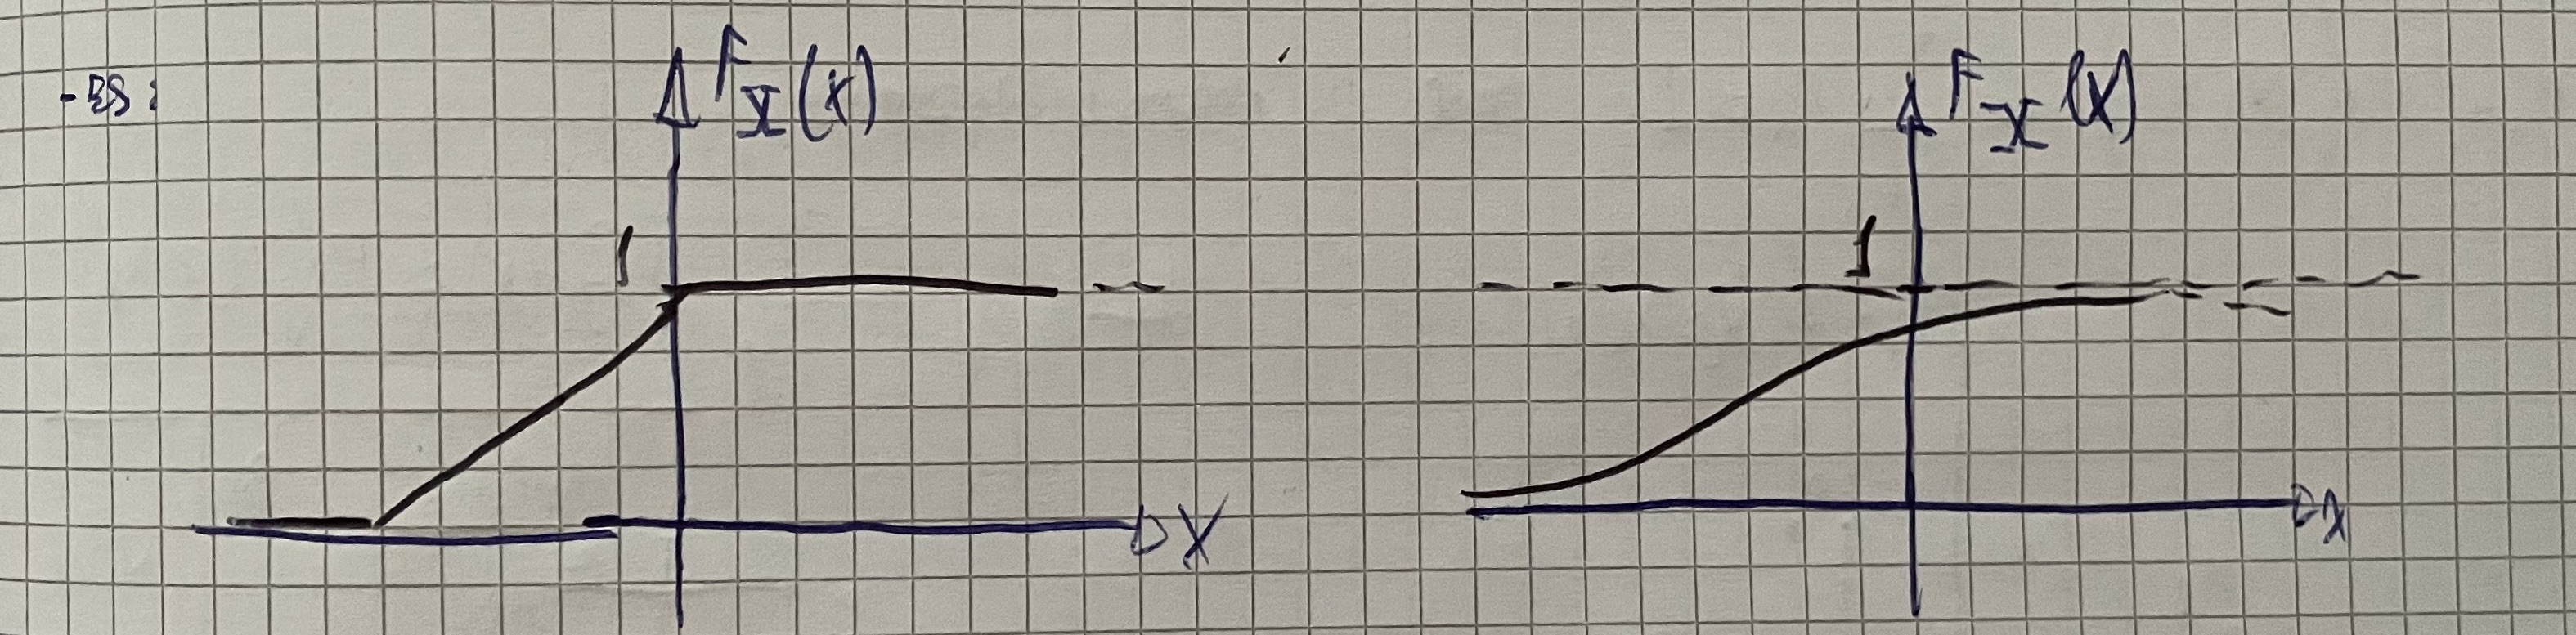
\includegraphics[scale=0.12]{images/28.prop4CDF.jpeg}
    \end{figure}
    \item Nel caso di una V.A. discreta, la CDF è continua a destra: \\
    $F_X(x) = F_X(x^+) = \lim_{h \to 0^+} F_X(x+h)$ \\
    $F_X(x+h) = P\big\{ X \leq x+h \big\} = P \big\{ X \leq x \big\} + \underset {\text{Per } h \to 0^+\text{ diventa un evento nullo: } \phi}{P \big\{ x < X \leq h \big\}}$ \\
    $= {\color{green}\underline{F_X(x)}} + \underset {\text{Per } h \to 0^+\text{ diventa un evento nullo: } \phi}{\underline{P \big\{ x < X \leq h \big\}}}$
    \begin{figure}[ht]
    \centering
    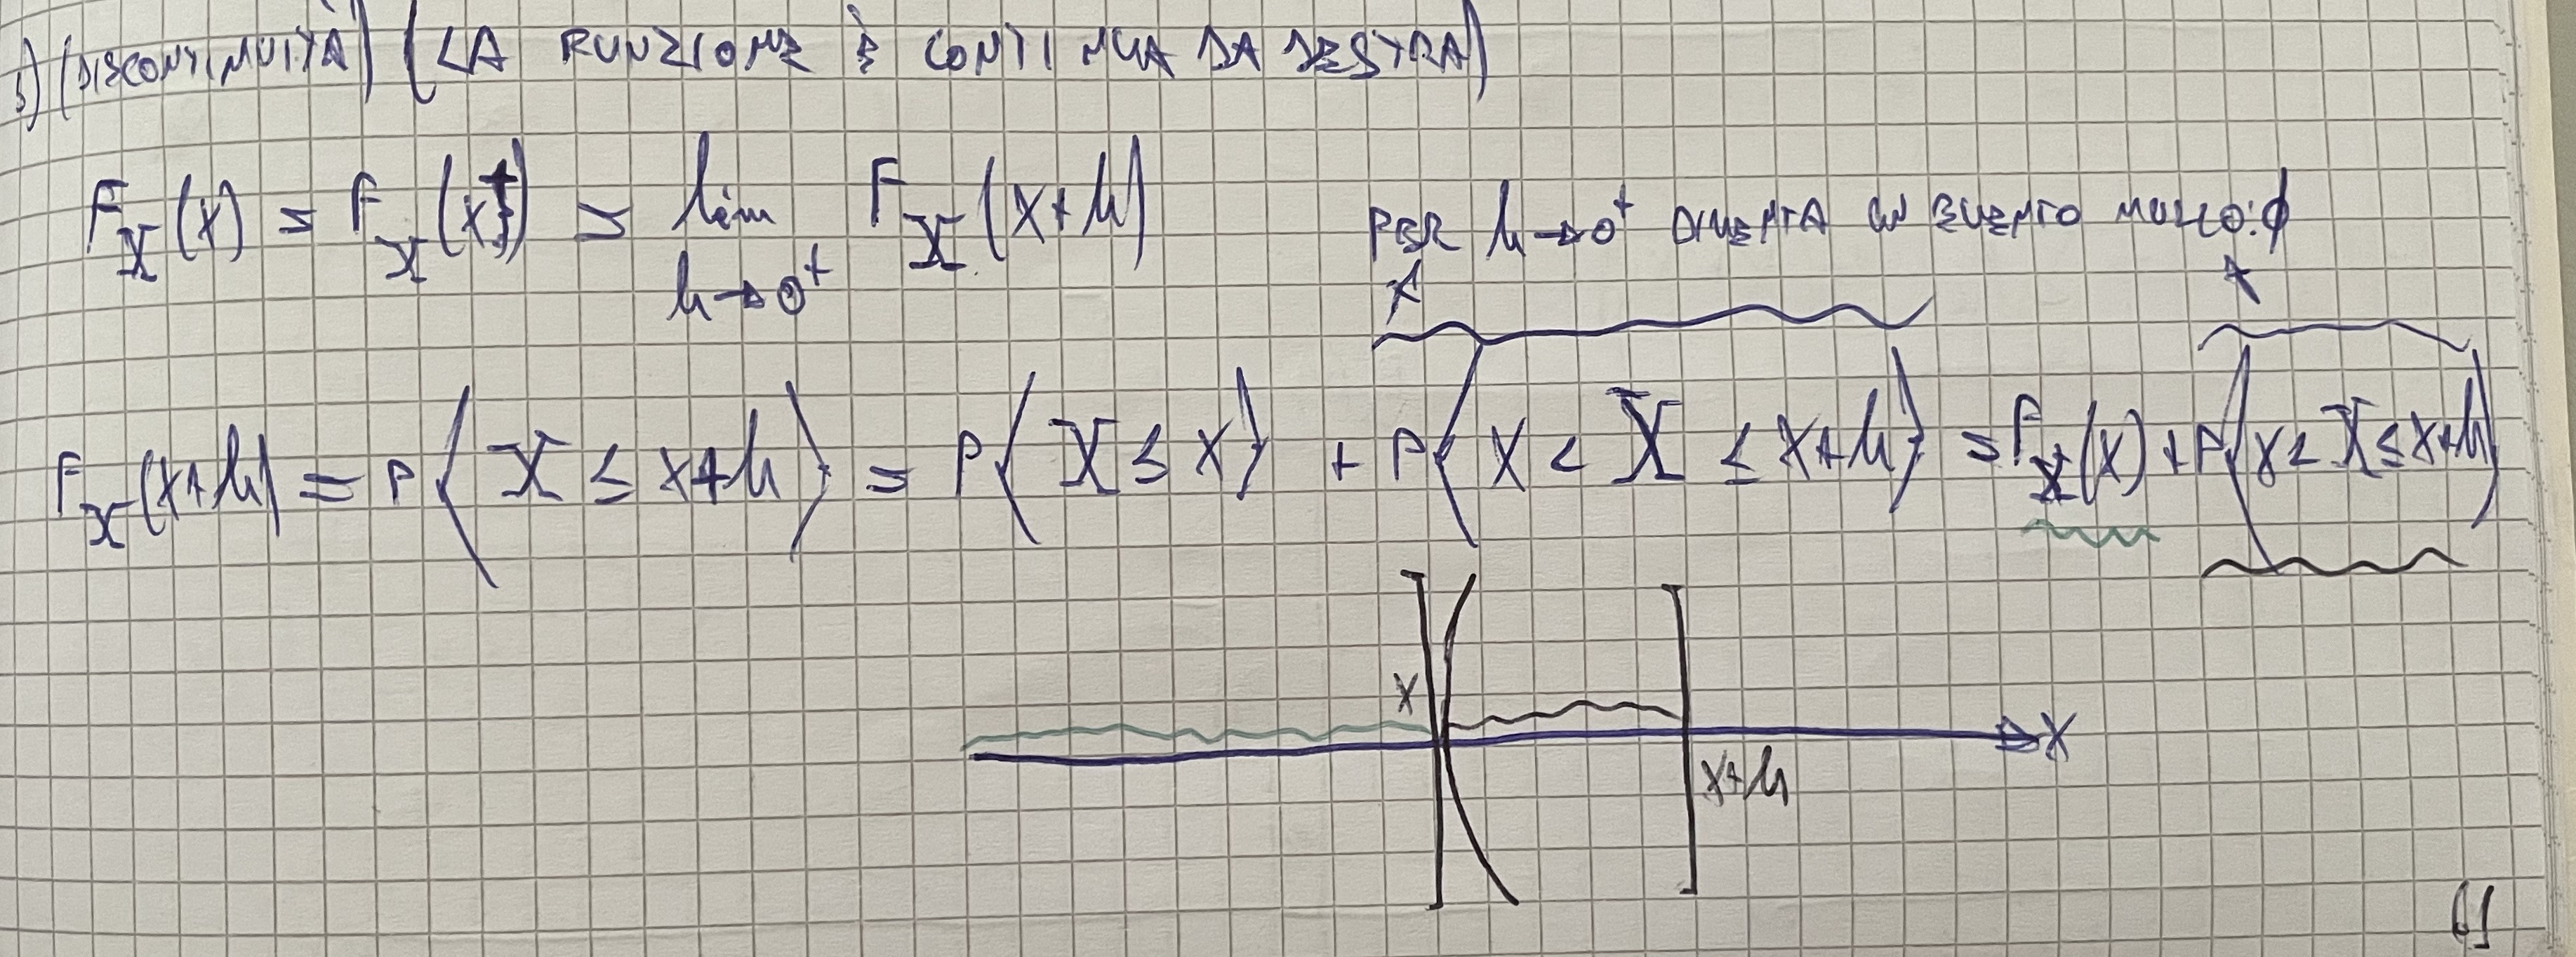
\includegraphics[scale=0.12]{images/29.prop5CDF.jpeg}
    \end{figure}
    \item La CDF presenta dei punti di discontinuità: \\
    $F_X(x) = F_X(x-h) + P\big\{ x-h < X \leq x\big\} $ \\
    $\implies P \big\{ X \leq x \big\} = P \big\{ X \leq x-h \big\} + P\big\{ x-h < X \leq x\big\}$ \\
    In ambo i membri faccio in modo che $h \to 0^+$ \\
    $\implies F_X(x^+) \left( = F_X(x)\right) = F_X(x^-) + P\big\{ X = x\big\}$ \\
    $\implies F_X(x^+) - F_X(x^-) = P\big\{ X = x\big\}$
    \paragraph{\underline{Esempio}}
    \begin{figure}[ht]
    \centering
    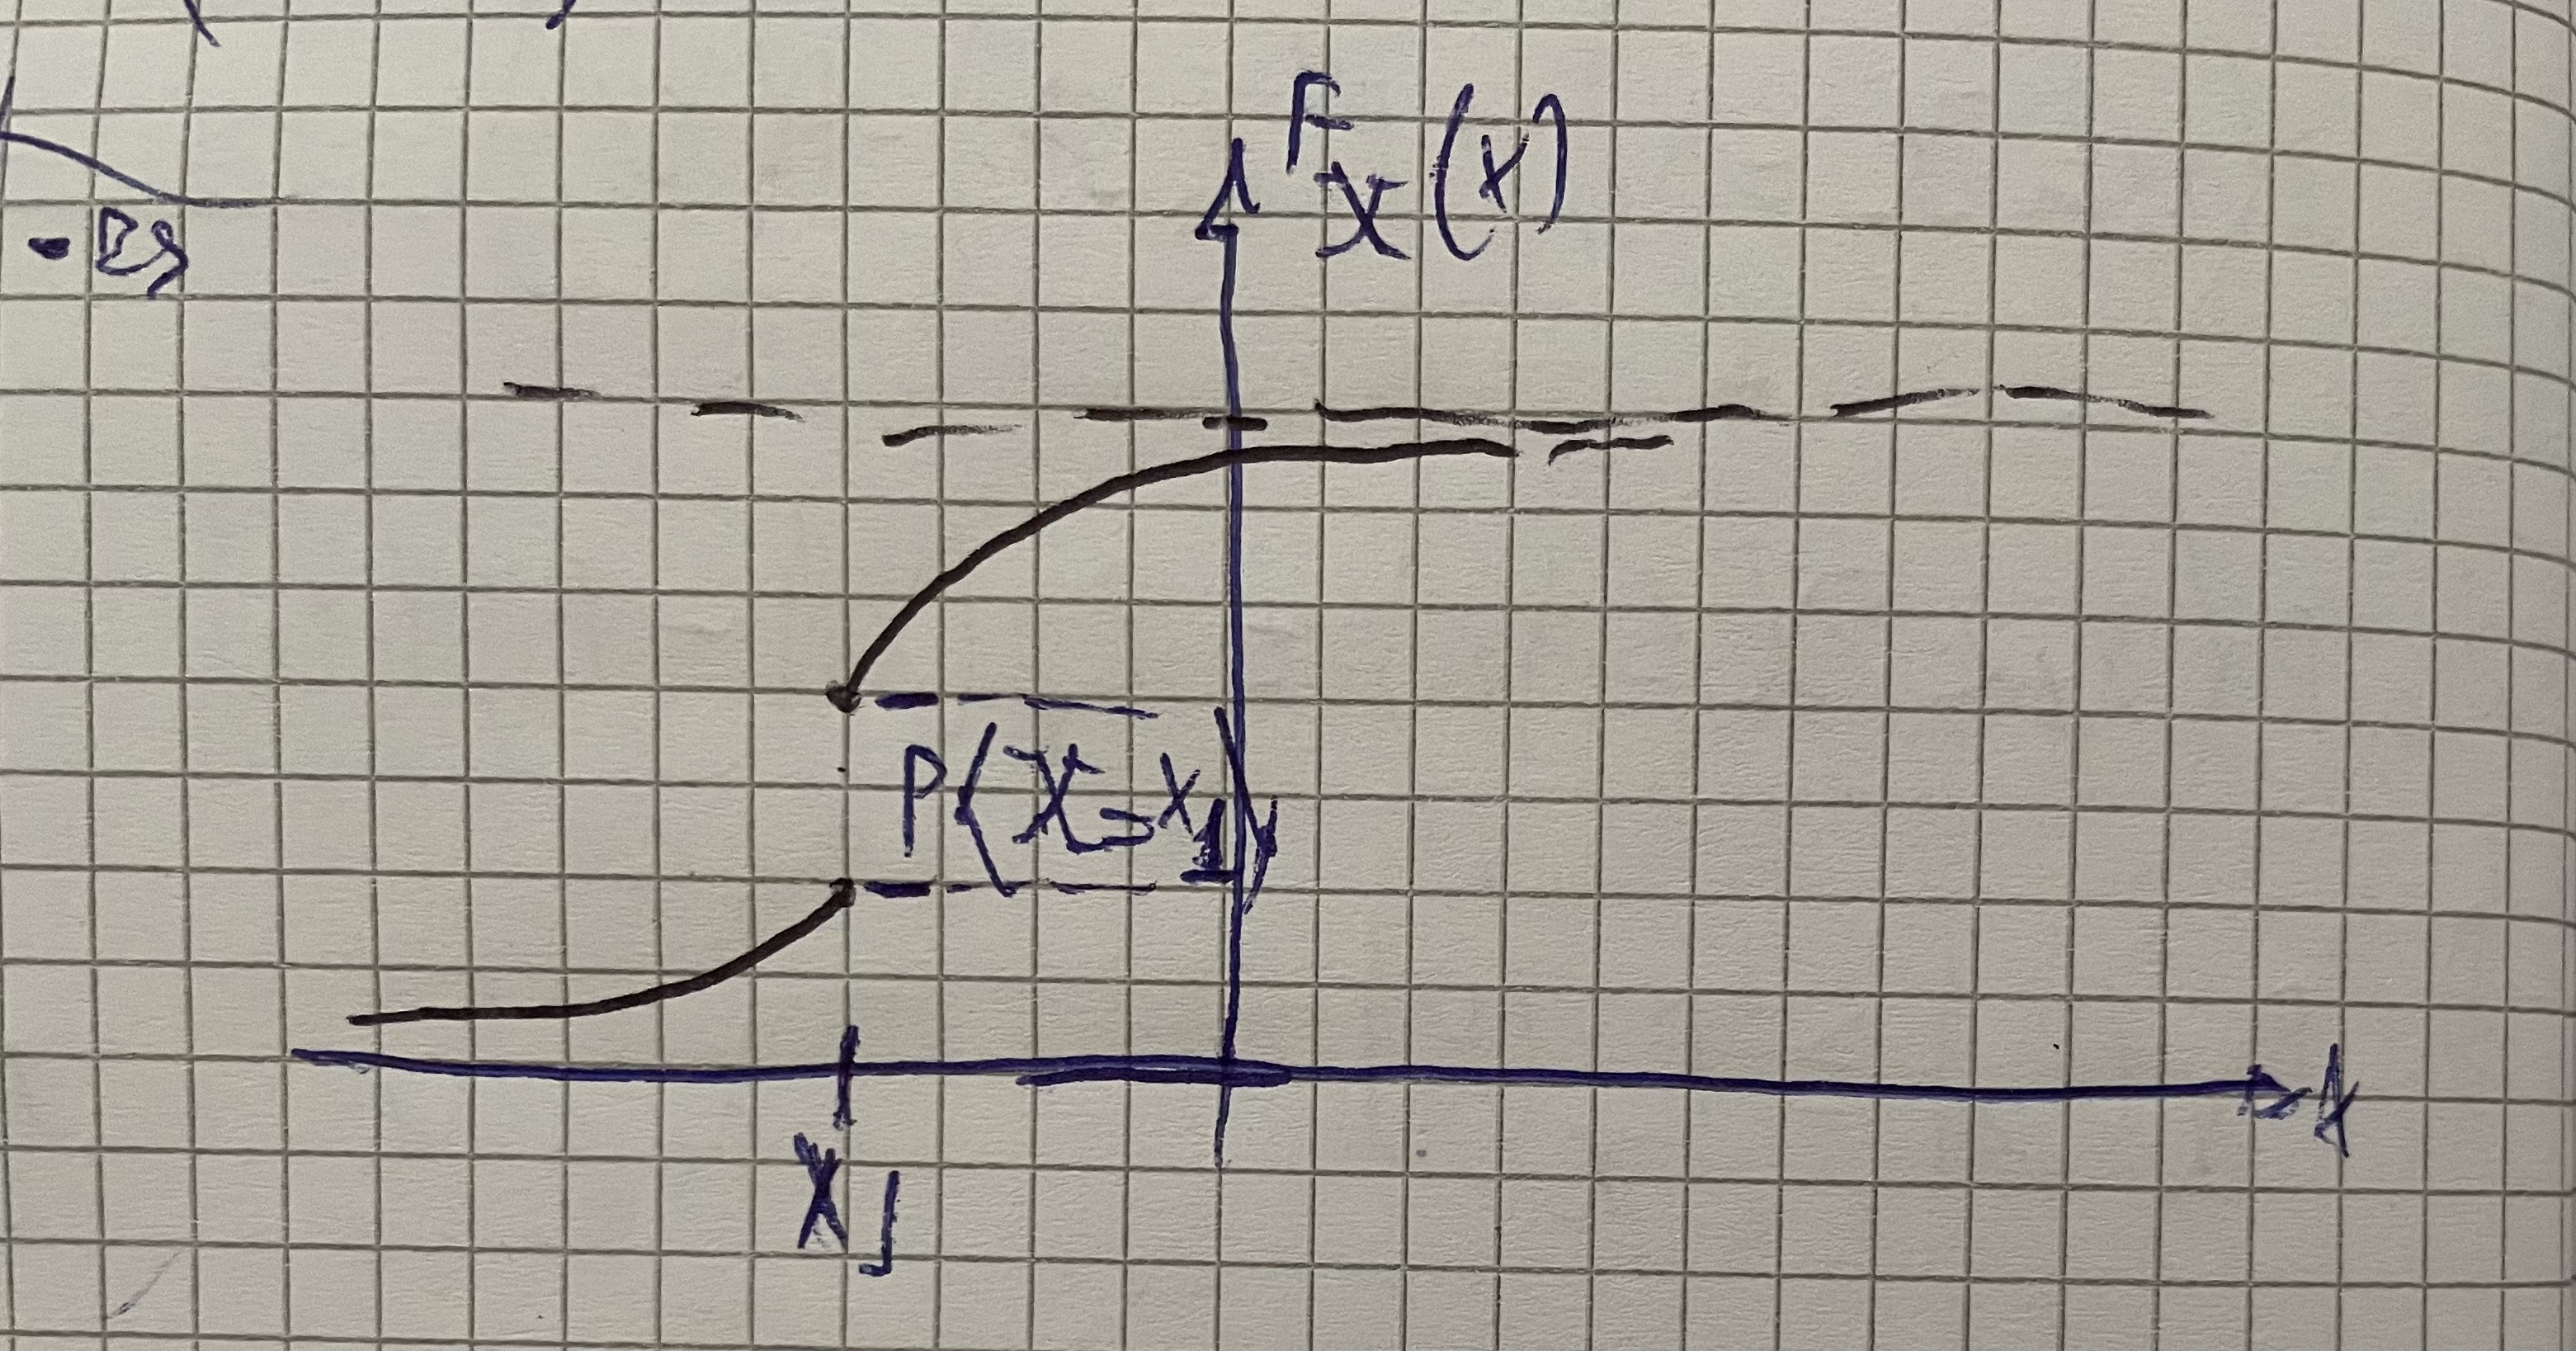
\includegraphics[scale=0.12]{images/30.prop6CDF.jpeg}
    \end{figure}
\end{enumerate}

\subsection{Variabili Aleatorie Discrete}
\begin{tabular}{|p{13cm}}
Una V.A. discreta è un tipo di variabile aleatoria che può assumere solo valori finiti infinitamente numerabili.
\end{tabular} \\
Vale la proprietà di normalizzazione: $P_i = P\big\{ X = x_i \big\} = \sum_i P_i = 1$ \\
Dove $P_i$ è detta \textbf{massa di probabilità} \\
Le V.A discrete sono caratterizzate da una CDF fatta nel seguente modo: $F_X(x) = \sum_i P_i \cdot u(x+x_i)$
\subsubsection{\underline{Grafico}}
\begin{figure}[ht]
\centering
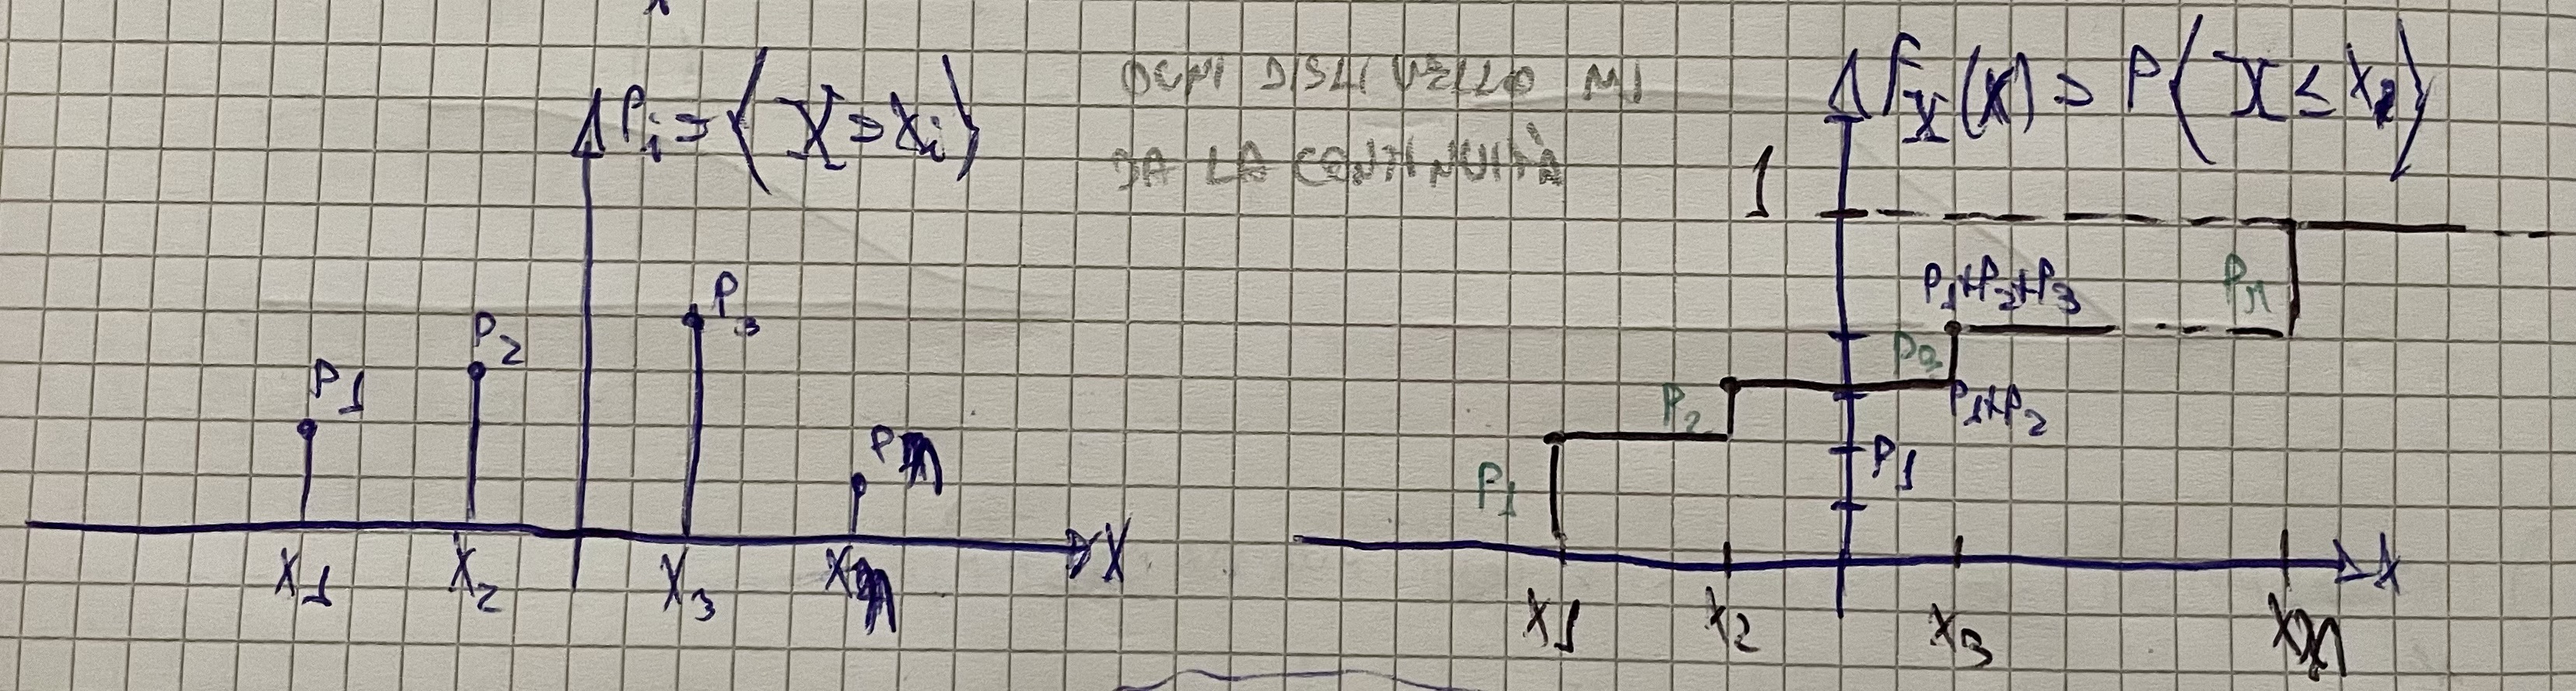
\includegraphics[scale=0.12]{images/31.VA_Discrete.jpeg}
\end{figure}
\newpage
\subsubsection{\underline{Esempio(Dado)}}
\begin{figure}[ht]
\centering
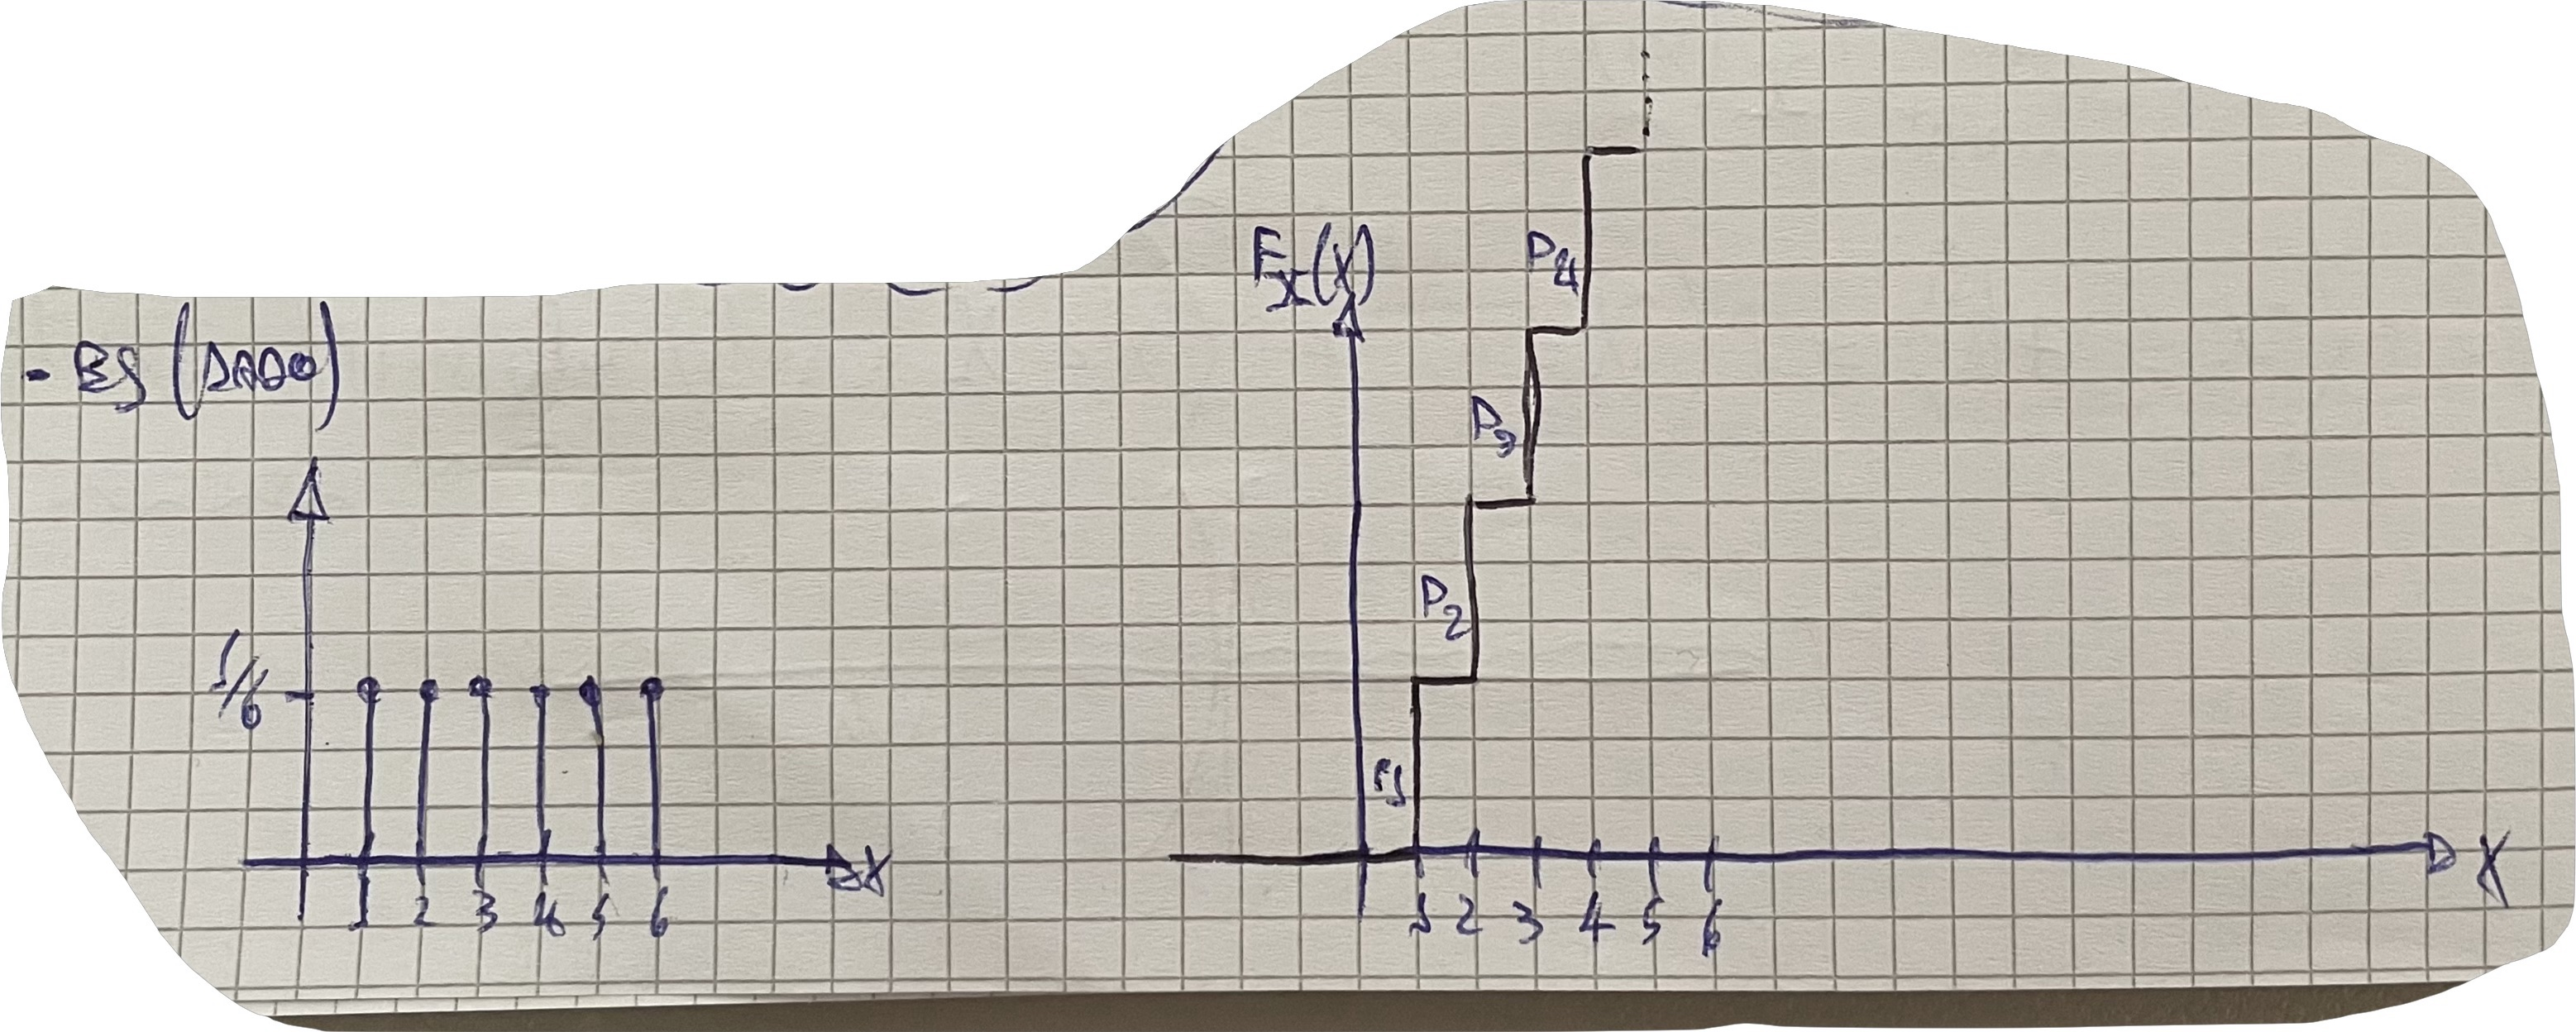
\includegraphics[scale=0.12]{images/32.VA_DiscEs.jpeg}
\end{figure}

\subsection{Funzione Indicatrice (V.A. di Bernoulli)}
\begin{tabular}{|p{13cm}}
Una variabile aleatoria di Bernoulli è una V.A. discreta che però può assumere solo due valori: 
\[I = \begin{cases}
0 \;\;\text{ se } a \in \overline A\\
1 \;\;\text{ se } a \in A
\end{cases}
\;\;
\bigg|
\;\;
\big[ P(A) = P\big]\]
Grazie alla V.A. di Bernoulli possiamo definire una CDF $\left(F_I(i)\right)$ che ci fa capire se un evento si è verificato o no.
\end{tabular} \\
Se una V.A. è di Bernoulli la indichiamo con $X \in \mathcal{B}er (P)$ \\
Nell’immagine di seguito vengono rappresentate graficamente una V.A. di Bernoulli e la sua CDF:
\begin{figure}[ht]
\centering
\includegraphics[scale=0.12]{images/32b.VA_Bernoulli.jpeg}
\end{figure}

\subsection{Variabile Aleatoria Binomiale}
\begin{tabular}{|p{13cm}}
Una variabile aleatoria Binomiale è una V.A. discreta che ci permette di definire il numero di $k$ successi in $n$ prove:
\[P_k = P(X = k) = \left(\begin{matrix} n \\ k \end{matrix}\right) \cdot P^k \cdot (1-P)^{n-k}\]
Dove $P_k$ è la massa di probabilità.
\end{tabular} \\
Se una V.A. è binomiale la indichiamo con $X \in \mathcal{B} $ 
\subsubsection{\underline{Esempio}}
Variabile aleatoria discreta con un’infinità di di valori numerabili.
\begin{figure}[ht]
\centering
\includegraphics[scale=0.12]{ese/13.jpeg}
\end{figure}

\subsection{Variabili Aleatorie Continue}
\begin{tabular}{|p{13cm}}
Una variabile aleatoria continua è una qualsiasi V.A. dotata di una CDF continua(senza discontinuità).
\end{tabular} \\
Tutti i punti hanno probabilità $= 0$
\subsubsection{\underline{Esempio(Calcolo probabilità tramite PDF)}}
$\begin{matrix}
P \big\{ x_1 < X \leq x_2 \big\} = F_X(x_2) - F_X(x_1) \\
P \big\{ x_1 \leq X \leq x_2 \big\} = F_X(x_2) -F_X(x_1) \\
P \big\{ x_1 \leq X < x_2 \big\} = F_X(x_2) -F_X(x_1) \\
P \big\{ x_1 < X < x_2 \big\} = F_X(x_2) -F_X(x_1)
\end{matrix}$

\subsection{PDF: Funzione di Densità di Probabilità}
\begin{tabular}{|p{13cm}}
La PDF o Probability Density Function viene definita come: 
\[f_X(x) = \frac{dF_X(x)}{dx}\]
Nell’associare ai risultati di un esperimento un valore numerico si costruisce una variabile casuale (o aleatoria, o stocastica).
Ogni variabile casuale ha una corrispondente distribuzione di probabilità. \\ \\
In caso di variabile discreta la distribuzione di probabilità specifica tutti i possibili risultati della variabile insieme alla probabilità che ciascuno di essi si verifichi. \\ \\
In caso di variabile continua la distribuzione di probabilità
consente di determinare la probabilità associata ad intervalli
di valori.
\end{tabular} \\
\subsubsection{\underline{Proprietà}}
\begin{enumerate}
    \item $f_X(x) \geq 0$
    \item $P \big\{ x_1 < X \leq x_2 \big\} = F_X(x_2) - F_X(x_1) = \int_{x_1}^{x_2} f_X(x) dx$
    \item Se nella proprietà numero 2 poniamo $x_1 \to -\infty$ e $x_2 = x$, otteniamo: \\
    $P \big\{ X \leq x \big\} = F_X(x) = \int_{-\infty}^{x} f_X(x) dx$
    \item Proprietà di normalizzazione: $F_X(+\infty) = 1 \implies \int_{-\infty}^{+\infty} f_X(x) dx = 1$
    \item Se nella proprietà numero 2 poniamo $x_1 = x$ e $x_2 = x + dx$, otteniamo: \\
    $P \big\{ x < X \leq x + dx \big\} =  f_X(x) dx$
\end{enumerate}

\subsection{Delta di Dirac e V.A.}
Utilizzando la delta di Dirac possiamo calcolare l’integrale e la derivata nei punti di discontinuità di una funzione di probabilità (CDF a gradini). \\ \\
Posso definire una PDF fatta cosi(PDF per V.A. discrete):
\begin{figure}[ht]
\centering
\includegraphics[scale=0.12]{images/33.V.A.Dirac.jpeg}
\end{figure}
Nella posizioni dove si trova la delta di Dirac, sono rappresentati i valori che la V.A. può assumere. \\
Per essere più precisi, l’area della delta (ovvero la loro “altezza”) rappresenta il valore che assume la V.A.
\[P \big\{ {\color{green}a} < X < {\color{green}b} \big\} = P_2 + P_3 = \int_{a}^{b} f_X (x) dx\]
Nel caso in cui ponessimo $b = x_3$ otterremmo $\int_{a}^{b^-} f_X(x) dx = P_2$ e $\int_{a}^{b^+} f_X(x) dx = P_2 + P_3$

\subsection{Variabili Aleatorie Miste}
Una variabile aleatoria mista può assumere sia valori discreti che valori continui ed è caratterizzata da una CDF continua ma con dei punti di discontinuità e da una PDF con tratti continui e una o più delta di Dirac.
\subsubsection{\underline{Grafico}}
\begin{figure}[ht]
\centering
\includegraphics[scale=0.12]{images/34.VA_Miste.jpeg}
\end{figure}
\subsubsection{\underline{Esempio}}
\begin{figure}[ht]
\centering
\includegraphics[scale=0.12]{ese/14.jpeg}
\end{figure}

\subsection{Variabili Aleatorie Uniformi}
Una variabile aleatoria uniforme è una V.A. che attribuisce la stessa probabilità a tutti i punti in un determinato intervallo e vengono definite come:
\[X \in \mathcal{U}(a,b)\]
Il grafico della sua PDF è semplicemente un impulso rettangolare, poiché assume un valore nel dato intervallo e vale $0$ altrove.

\subsection{Variabili Aleatorie Esponenziali (Negative)}
\begin{tabular}{|p{13cm}}
Una variabile aleatoria esponenziale, all’esponente ha un valore negativo, altrimenti il suo integrale non avrebbe area unitaria($=1$). \\
Le V.A. esponenziali vengono indicate con:
\[X \in \varepsilon(\eta) \;\text{ oppure }\; \color{red} X \in \varepsilon(\lambda)\]
Dove $\lambda$ è detto valor medio. \\
Le V.A. esponenziali sono caratterizzate da una PDF del seguente tipo:
\[f_X(x) = \frac 1 \eta \cdot e^{- \frac x \eta} \cdot u(x) = \color{red} \lambda \cdot e^{-\lambda \cdot x} \cdot u(x)\]
\end{tabular} \\
Possiamo notare che una V.A. esponenziale è definita da un “parametro” che verrà introdotti meglio nel capitolo 5.20. \\ \\
Di seguito il grafico della PDF:
\begin{figure}[ht]
\centering
\includegraphics[scale=0.12]{images/35.PDF_VA_exp.jpeg}
\end{figure} ~\\
La CDF invece si può calcolare come: \\
$F_X(x) = \int_{- \infty}^{x} f_X(\alpha) d\alpha = 
\begin{cases}
0 \;\;\text{ se } x<0 \\
\frac 1 \eta \cdot \int_{0}^{x}e^{- \frac \alpha \eta} dx \;\;\text{ se } x \geq 0
\end{cases}$ \\
Da notare come l’integrale della PDF va da $0$ a $x$ poiché la PDF è caratterizzata da un gradino unitario. \\
$= 
\begin{cases}
0 \;\;\text{ se } x<0 \\
-e^{- \frac \alpha \eta} \Big|_{0}^{x} \;\;\text{ se } x \geq 0
\end{cases}
=
\begin{cases}
0 \;\;\text{ se } x<0 \\
-e^{- \frac x \eta} +1 \;\;\text{ se } x \geq 0
\end{cases}$ \\
Che può essere riscritto come: 
\[F_X(x) = \Big[1 - e^{-\frac x \eta }\Big] \cdot u(x)\]
Di seguito il grafico della CDF:
\begin{figure}[ht]
\centering
\includegraphics[scale=0.10]{images/36.CDF_VA_exp.jpeg}
\end{figure}

\subsection{Variabili Aleatorie Normali o Gaussiane}
\begin{tabular}{|p{13cm}}
Una variabile aleatoria gaussiana (o normale) è considerata la più importante “distribuzione” Statistica per le innumerevoli Applicazioni e per le rilevanti proprietà di cui gode e viene indicata in questo modo:
\[X \in \mathcal{N}\left( \eta, \sigma^2 \right)\]
Le V.A. gaussiane sono caratterizzate dalla loro PDF fatta in questo modo:
\[f_X(x) = \frac{1}{\sqrt{2 \pi \sigma ^2}} \cdot e^{- \frac{(x-\eta)^2}{2 \sigma^2}}\]
\end{tabular} \\
Possiamo notare che una V.A. gaussiana è definita da due “parametri” che verranno introdotti meglio nei capitoli 5.20 e 5.21. \\ \\
Di seguito il grafico della PDF:
\begin{figure}[ht]
\centering
\includegraphics[scale=0.12]{images/37.PDF_VA_gauss.jpeg}
\end{figure} ~\\
\begin{tabular}{|p{13cm}}
In particolare, tramite le V.A. gaussiane possiamo comprendere meglio come sono fatte le funzioni $Q$ e $G$, ovvero:
\begin{itemize}
    \item $G(x) = \int_{- \infty}^{x} \frac{1}{\sqrt{2 \pi}} \cdot e^{- \frac{t^2}{2}} dt$
    \item $Q(x) = \int_{x}^{+ \infty} \frac{1}{\sqrt{2 \pi}} \cdot e^{- \frac{t^2}{2}} dt$
\end{itemize}
Inoltre, si può facilmente notare che $Q(x) = 1 -G(x)$
\end{tabular} \\ \\
Calcoliamo adesso la CDF di una V.A. gaussiana: \\
$F_X(x) = \int_{- \infty}^{x} f_X(\alpha) d\alpha = \int_{- \infty}^{x} \frac{1}{\sqrt{2 \pi \sigma^2}} \cdot e^{- \frac{(\alpha - \eta)^2}{2 \sigma^2}} d\alpha$ \\
Eseguo un cambio di variabile: $\beta = \frac{\alpha - \eta}{\sigma}$ e otteniamo \\
$\int_{- \infty}^{\frac{x-\eta}{\sigma}} \frac{1}{\sqrt{2 \pi }} \cdot e^{- \frac{\beta^2}{2 }} d\beta = G\left(\frac{x - \eta}{\sigma}\right) =$ $\color{red}1 - Q\left( \frac{x - \eta}{\sigma} \right)$
\subsubsection{\underline{Esempio 1}}
\begin{figure}[ht]
\centering
\includegraphics[scale=0.12]{ese/15.jpeg}
\end{figure}
\subsubsection{\underline{Esempio 2}}
\begin{figure}[ht]
\centering
\includegraphics[scale=0.12]{ese/16.jpeg}
\end{figure}

\subsection{Trasformazioni di Variabili Aleatorie}
Sullo stesso esperimento possiamo definire più variabili aleatorie ad esempio $X$ e $Y$, come possiamo notare nell'immagine di seguito.
\begin{figure}[ht]
\centering
\includegraphics[scale=0.12]{images/38.Due_VA_un_Esper.jpeg}
\end{figure} ~\\
Quindi si dice che, data una variabile aleatoria $X$, si definisce trasformazione della variabile aleatoria $X$ una funzione $g$ che da vita ad una nuova V.A. $Y$ che può essere descritta come: $Y = g(X)$ \\ \\
Il problema che ci poniamo è quello di calcolare la funzione di densità (PDF) e/o la funzione cumulata (CDF) della trasformazione $g$ essendo nota la PDF della V.A. $X$ di partenza. \\
Per farlo esistono due metodi, ovvero il \textbf{metodo grafico} e \textbf{Teorema fondamentale}, ma per ora ci concentreremo solo sul primo metodo.
\subsubsection{\underline{Esempio}}
Ora un banale esempio per capire come si può definire una funzione $g$: \\
Esperimento: Lancio di una freccetta \\
$X$: Distanza freccetta centro \\
$Y$: Distanza freccetta bordo 
\newpage
\begin{figure}[ht]
  \begin{subfigure}{.5\textwidth}
  \centering
    \includegraphics[width=.9\linewidth]{images/39.Esempio1Trasf1.jpeg}
  \end{subfigure}
  \begin{subfigure}{.5\textwidth}
  \centering
    \includegraphics[width=.9\linewidth]{images/40.Esempio1Trasf2.jpeg}
  \end{subfigure}
\end{figure} ~\\
La legge che lega $X$ e $Y$ è $X(a) = R - Y(a)$ \\
Da questa possiamo ricavare che $Y(a) = R - X(a) \implies y = g(x_1) = R-X$

\subsection{Calcolare la V.A. $Y$ data la V.A. $X$}
Se io ho una V.A. $X$ definita da una CDF $F_X(x)$ o da una PDF $f_X(x)$ e conosco $g(x)$, allora posso calcolare $Y$ e di conseguenza anche $F_Y(y)$ e $f_Y(y)$. \\
Posso quindi scrivere che $Y=g(X)$ 
\subsubsection{\underline{Esempio(Y discreta e X continua)}}
Voglio calcolare una V.A. $Y$ fatta in questo modo: $y_1,y_2,...,y_n.$ \\
In questo caso la nostra V.A. $X$ è definita da una CDF $F_x(x)$ o da una PDF
$f_X(x)$ generiche. \\
Prendo quindi una funzione $g(x)$ fatta in questo modo:
\begin{figure}[ht]
\centering
\includegraphics[scale=0.12]{images/41.EsTrasf1.jpeg}
\end{figure} ~\\
Dall'immagine possiamo facilmente capire che $Y$ può assumere solo 2 valori,
ovvero $y_1=0$ e $y_2=1$, quindi è facile dedurre che $Y\in\mathcal{B}er(x)$. \\
$Y$ sarà definita solo quando avrò calcolato le probabilità: $P \big\{Y = 0\big\}$ e $P \big\{Y = 1\big\}$. \\
Per calcolare le probabilità di $Y$ mi riconduco a quelle di $X$: \\
$P \big\{Y = 0\big\} = P \big\{X \leq 0\big\} = F_X(0) = \int_{- \infty}^{0} f_X(x) dx \;\;\;\; \big[\mathcal{G}(0) \;\; \big\{x < 0\big\}\big]$ \\
$P \big\{Y = 1\big\} = 1 - P \big\{Y = 0\big\} =  1 - P \big\{X \leq 0\big\} = 1-F_X(0) = \int_{0}^{+ \infty} f_X(x) dx \;\;\;\; \big[\mathcal{G}(1) \;\; \big\{x \geq 0\big\}\big]$ \\
\subsubsection{\underline{Esempio(Y discreta e X discreta)}}
Come nell’esempio di prima voglio calcolare una V.A. $Y$ fatta in questo modo: $y_1,y_2, \dots , y_n$ \\
Questa volta però ho una V.A $X$ discreta definita in questo modo: $X = \big\{0, \pm 1 , \pm 2 \big\} $ \\
$\implies P\big\{X = 0\big\} = \frac 15 \;\big|\;  P\big\{X = +1\big\} = \frac 15 \;\big|\;  P\big\{X = +2\big\} = \frac 15 \;\big|\;  P\big\{X = -1\big\} = \frac 15 \;\big|\;  P\big\{X = -2\big\} = \frac 15$ \\
Noi sappiamo che $Y=g()X$ e che in questo caso $g(x) = x^2$ $\implies Y = \big\{0,1,4\big\}$ \\
Quindi, come nell’esempio precedente ci basta calcolare le probabilità di $Y$ riconducendosi a quelle di $X$: \\
$P \big\{Y = 0 \big\} = P \big\{X = 0 \big\} = \frac 15 $ \\
$P \big\{Y = 1 \big\} = P \big\{X = +1 \big\} + P \big\{X = -1 \big\} = \frac 25 $ \\
$P \big\{Y = 4 \big\} = P \big\{X = +2 \big\} + P \big\{X = -2 \big\} = \frac 25 $

\subsection{Calcolare la V.A. Discreta $Y$ data la V.A. $X$ Generica}
Per calcolare una V.A. $Y$ discreta indipendentemente dal tipo della V.A. $X$ devo calcolare: \\
$P\big\{ Y=y_i\big\} = \underset{\mathcal{G}(y_i)}{\underbrace{P \big\{ x \in \mathbb{R} \big| g(x) = y_i \big\}}}$ \\
A seconda della tipologia di $X$ avremo:
\begin{itemize}
    \item $= \int_{\mathcal{G}(y_i)} f_X(x) dx$ se $X$ è continua
    \item $= \int_{\mathcal{G}(y_i)} P \big\{ X=x_i\big\}dx$ se $X$ è discreta
\end{itemize}

\subsection{Calcolare la V.A. Continua $Y$ data la V.A. $X$ Generica}
Per calcolare una V.A. $Y$ continua indipendentemente dal tipo della V.A. $X$ devo calcolare: \\
$F_Y(y) = P \big\{ Y \leq y \big\} = \underset{\mathcal{I}(y)}{\underbrace{P \big\{ x \in \mathbb{R} \big| g(x) \leq y \big\}}} = \int_{\mathcal{I}(y)} f_X(x) dx$ \\
Tendendo sempre a mente che $f_Y(Y) = \frac{dF_Y(y)}{dy}$.

\subsection{Regola Importante per gli Esercizi (Funzioni a due Variabili)}
Se $z(y) = \int_{\alpha(y)}^{\beta(y)} h(x,y) dx$ \\
Posso riscrivere il tutto come: \\
$\frac{dz(y)}{dy} = h \left( \beta(y), y\right) \cdot \frac{d\beta(y)}{dy} - h \left( \alpha(y), y\right) \cdot \frac{d\alpha(y)}{dy} + \int_{\alpha(y)}^{\beta(y)} \frac{dh(x,y)}{dy} dx$
\subsubsection{\underline{Esempio}}
\begin{figure}[ht]
\centering
\includegraphics[scale=0.14]{ese/17.jpeg}
\end{figure} 
\begin{figure}[ht]
\centering
\includegraphics[scale=0.11]{ese/17a.jpeg}
\end{figure} 
\begin{figure}[ht]
\centering
\includegraphics[scale=0.13]{ese/17b.jpeg}
\end{figure} 
\clearpage
\subsection{Teorema Fondamentale}
\subsubsection{\underline{Caso g(x) monotona crescente}}
Supponiamo che $g(x)$ sia una funzione monotona crescente:
\begin{figure}[ht]
\centering
\includegraphics[scale=0.13]{images/42.TeoFondMonoCresc.jpeg}
\end{figure} ~\\
Quindi avremo che: \\
$f_Y(y) dy = P \big\{ y \leq Y \leq y+ dy \big\} = P \big\{ x \leq X \leq x+ dx \big\} = f_X(x) dx$ \\
Quindi possiamo concludere generalizzando che: $f_Y(y) = \frac{f_X(\overline x)}{g^{'}(\overline x)} \bigg|_{\overline x = g^{-1}(y)}$
\subsubsection{\underline{Caso g(x) non monotona crescente}}
Supponiamo adesso che $g(x)$ non sia una funzione monotona crescente:
\begin{figure}[ht]
\centering
\includegraphics[scale=0.13]{images/43.TeoFondNonMonoCresc.jpeg}
\end{figure} ~\\
Quindi avremo che: \\
$f_Y(y) dy = P \big\{ y \leq Y \leq y+ dy \big\} = P \big\{ x_1 \leq X \leq x_1 + dx \big\} + P \big\{ x_2 - dx \leq X \leq x_2  \big\} + P \big\{ x_3 \leq X \leq x_3 + dx \big\}$ \\
$= f_X(x_1) dx - f_X(x_2) dx + f_X(x_3) dx$ \\
Da notare come $f_X(x_2)$ è messa con il segno meno, poiché nel grafico ha pendenza negativa. \\
Quindi possiamo concludere generalizzando che:
\[\color{red} f_Y(y) = \sum_{x_i} \frac{f_X(x_i)}{| g^{'}(x_i)|} \bigg|_{ x_i = g^{-1}(y)}\]
\subsubsection{\underline{Caso Y discreta}}
Nel caso in cui $Y$ sia una V.A. discreta: $\mathcal{G}(y) = \big\{ x \in \mathbb{R} \big| g(x) = y\big\}$ possiamo riscrivere la formula come:
\[ f_Y(y) = \sum_{x_i : g(x)=y} \frac{f_X(x_i)}{| g^{'}(x_i)|} \]
\subsubsection{\underline{Esempio 1}}
\begin{figure}[ht]
\centering
\includegraphics[scale=0.15]{ese/18.jpeg}
\end{figure}
\clearpage
\subsubsection{\underline{Esempio 2}}
\begin{figure}[ht]
\centering
\includegraphics[scale=0.15]{ese/19.jpeg}
\end{figure}
\clearpage
\subsubsection{\underline{Esempio 3}}
\begin{figure}[ht]
\centering
\includegraphics[scale=0.12]{ese/20.jpeg}
\end{figure}
\begin{figure}[ht]
\centering
\includegraphics[scale=0.11]{ese/20a.jpeg}
\end{figure}
\clearpage
\subsubsection{\underline{Esempio 4}}
\begin{figure}[ht]
\centering
\includegraphics[scale=0.13]{ese/21.jpeg}
\end{figure}

\subsection{Problema Inverso (Alle Trasformazioni di V.A.)}
Come abbiamo potuto notare nel paragrafo precedente, abbiamo spiegato come ricavare una seconda V.A. da una prima data una funzione $g(x)$, in questo capitolo ci poniamo il problema inverso, ovvero: \\
data la descrizione di due V.A. $X$ e $Y$ con delle generiche CDF e PDF $F_X(x),F_Y(y),f_X(x) \text{ e } f_Y(y)$, calcolare la funzione $g(x)$. \\
Per semplificare il tutto dividiamo il problema in due sotto-problemi: 
\begin{enumerate}
    \item Dalla V.A. $X$ voglio passare ad una V.A. uniforme tramite $g(x)$, quindi in questo caso il problema è proprio trovare $g(x)$, in altre parole: $X \to U \in \mathcal{U}[0,1]$ \\
    Possiamo scrivere che $U = g(x) = F_X(x)$ che possiamo rappresentare nel seguente modo: 
    \begin{figure}[ht]
    \centering
    \includegraphics[scale=0.13]{images/44.ProblemaInverso.jpeg}
    \end{figure} ~\\
    Quindi ora devo dimostrare che $F_U(u) = u$: \\
    $F_U(u) = P \big\{ U \leq u \big\} = P \big\{ X \leq \overline x \big\} = F_X(\overline x) = F_X \big[ F_X^{-1}(u) \big] = u$ \\
    $\begin{matrix} 
    X \underset{F_X(x)}{\to} U & & X \underset{F^{-1}_X(u)}{\leftarrow} U \\
    & \Downarrow &
    \end{matrix}$
    \item $X \underset{F_X}{\to} U \underset{F^{-1}_{Y}}{\to} Y$ \\
    Tramite quello che abbiamo ottenuto dal primo passaggio possiamo calcolare la V.A $Y$.
\end{enumerate}

\subsection{Valor Medio}
$\eta$ (spesso indicato anche con $\lambda$) è detto \textbf{valor medio (media)}. 
Nel caso in cui il valor medio sia riferito ad una V.A. $X$ lo indichiamo con $\eta_x$. \\
Il valor medio è anche detto \textbf{indice di posizione}, poiché in probabilità è l’analogo fra baricentro in fisica, ovvero quel punto di equilibrio fra diversi punti con masse differenti, che generalmente viene calcolato come somma delle posizioni moltiplicate per le rispettive masse e divise per la massa totale, come possiamo notare dalla seguente immagine:
\begin{figure}[ht]
\centering
\includegraphics[scale=0.13]{images/45.VM_Baricentro.jpeg}
\end{figure} ~\\
Ovviamente, nel calcolo delle probabilità non dividiamo per la “massa totale” poiché la probabilità totale è 1 e quindi un qualsiasi valore diviso per 1 è uguale allo stesso valore. \\ 
Nel nostro caso, ovviamente, non parliamo di masse ma di probabilità, quindi ogni posizione, ovvero ogni valore della V.A. verrà moltiplicato con la propria probabilità. \\ \\
Calcolare il valor medio:
\begin{table} [ht]
    \centering
    \begin{tabular}{|c|c|}
         \hline
         V.A Discreta & V.A Continua\\
         \hline 
         $\eta_x = E(X) = \sum_{i=1}^{n}x_i \cdot f_X(x_i) $ & $\eta_x = E(X) = \int_{- \infty}^{+\infty}x \cdot f_X(x) \,dx $ \\
         \hline
    \end{tabular}
\end{table} \\
L’operatore $E$ è chiamato expectation, valore atteso o più comunemente in italiano scorretto “aspettazione”. \\
Nel caso di una V.A. esponenziale indica la posizione del grafico (generalmente 1° o 4° quadrante). \\
Nel caso di una V.A. gaussiana sta ad indicare se il grafico della PDF viene traslato a destra o a sinistra, nello specifico, se $\eta = 0$ il grafico sarà centrato, mentre invece, all’aumentare di $\eta$ il grafico si sposterà sempre di più a destra.
\subsubsection{\underline{Esempio (calcolare valor medio V.A. discreta)}}
Quindi $X= \big\{ x_1,x_2, \dots, x_n\big\}$ \\
Essendo $X$ una V.A. discreta sappiamo che la sua PDF è uguale a $f_X(x) = \sum_{i=1}^{n} p_i \cdot \delta(x-x_i)$ caratterizzata quindi dal seguente grafico:
\begin{figure}[ht]
\centering
\includegraphics[scale=0.13]{images/46.PDF_Discreta.jpeg}
\end{figure} \\
Calcoliamo adesso il valor medio: \\
$\eta_x = \int_{- \infty}^{+ \infty} x \cdot \sum_{i=1}^{n} p_i \cdot \delta(x-x_i) = \sum_{i=1}^{n} p_i \cdot \int_{- \infty}^{+ \infty} x \cdot \delta(x-x_i)$ \\
Utilizziamo il teorema del campionamento della delta e otteniamo: \\
$= \sum_{i=1}^{n} p_i \cdot x_i$ \\ \\
Supponiamo che le varie $x$ siano dei risultati di un infinito numero di lanci, possiamo quindi scrivere: $p_i = \frac{L(x_i)}{L}$ \\
Sostituendo ciò che abbiamo appena scritto nella formula otteniamo: $\lim_{L \to +\infty} \sum_{i=1}^{n} \frac{L(x_i)}{L} \cdot x_i$ \\ \\
Supponiamo quindi di aver fatto solo 2 lanci, utilizzando la forma appena scritta, il calcolo del valor medio risulterebbe esattamente uguale a quello del baricentro in fisica, ovvero una banale media aritmetica: $\frac{L(x_1) \cdot x_1 + L(x_2) \cdot x_2}{L}$

\subsection{Varianza}
$\sigma^2$ è detta \textbf{varianza} ed è uguale al quadrato della \textbf{deviazione standard}  o viceversa, la deviazione standard è uguale ala radice della varianza.
Nel caso in cui la varianza sia riferito ad una V.A. $X$ la indichiamo con $\sigma^2_x$. \\
La varianza è anche detta \textbf{indice di dispersione}, poiché indica come i valori si disperdono intorno al valor medio, più è piccola, più i valori saranno concentrati intorno al valor medio, più è grande, più i valori saranno dispersi intorno al valor medio: $\eta_x = \int_{0}^{+ \infty} \big[1 - F_X(x)\big] \,dx - \int_{- \infty}^{0} F_X(x) \,dx$ \\
Come si può appunto notare dal seguente grafico:
\begin{figure}[ht]
\centering
\includegraphics[scale=0.13]{images/47.Varianza.jpeg}
\end{figure} ~\\
Calcolare la varianza:
\begin{table} [ht]
    \centering
    \begin{tabular}{|c|c|}
         \hline
         V.A Discreta & V.A Continua\\
         \hline 
         $\sigma^2_x = E\big\{ (X-\eta_x)^2 \big\} = \sum_{i=1}^{n} p_i \cdot (x_i - \eta_x)^2$ & $\sigma^2_x = E\big\{ (X-\eta_x)^2 \big\} = \int_{- \infty}^{+\infty} (x-\eta_x)^2 \cdot f_X(x) \,dx $ \\
         \hline
    \end{tabular}
\end{table} \\
Notiamo come per il teorema fondamentale possiamo dire che: $Y = (X-\eta_x)^2 = g(X)$ \\ \\
Calcoliamo ora la deviazione standard: \\
$\sigma_x = \sqrt{E\big\{(X - \eta_x)^2\big\}} = \sqrt{\int_{-\infty}^{+\infty} (x-\eta_x)^2 \cdot f_X(x) \, dx }$ \\
NOTA BENE, la deviazione NON può essere calcolata nel seguente modo: \\
$\sigma_x = \sqrt{E\big\{(X - \eta_x)^2\big\}} \neq E\big\{ | X - \eta_x |\big\} = \int_{- \infty}^{+ \infty} | X - \eta_x | \cdot f_X(x) \, dx$ \\ \\
Nel caso di una V.A. gaussiana indica l’altezza e la larghezza del grafico della PDF, in particolare, più $\sigma^2$ sarà piccolo, più il grafico sarà alto e stretto, mentre invece più $\sigma^2$ sarà grande, più il grafico sarà schiacciato e largo. \\ \\
Valor medio e varianza potrebbero avere degli integrali (o delle serie) che non convergono e di conseguenza potrebbero non essere definiti come valori finiti (infinità numerabile di valori).
\subsubsection{\underline{Esempio}}
Si lancia una moneta 5 volte, se almeno 4 volte su 5 si presenta testa si vince, se invece si presenta meno di 4 volte si perde. \\
Si scommette una quantità $S$ di denaro, se si vince si prende una somma $S_1$ di denaro, se invece si perde, si perde una quantità $S_2$ di denaro. \\ \\
Posso utilizzare le prove ripetute per risolvere l’esercizio: \\
$\underset{k \text{ teste su 5 lanci}}{\underbrace{P \big\{ X = k\big\}}} = \left(\begin{matrix} 5 \\ k\end{matrix}\right) \cdot \left(\frac 12\right)^k \cdot \left(\frac 12\right)^{5-k} = \left(\begin{matrix} 5 \\ k\end{matrix}\right) \cdot \left(\frac 12\right)^5$ \\
Posso definire una V.A. $Y = \begin{cases}
+S_1 & \text{se si vince} \\
-S_2 & \text{se si perde} 
\end{cases}$ \\
Quindi: \\
$P\big\{Y = S_1 \big\} = \underset{\text{4 teste su 5 lanci}}{\underbrace{P\big\{X = 4 \big\}}} + \underset{\text{5 teste su 5 lanci}}{\underbrace{P\big\{X = 5 \big\}}}
=
\left(\begin{matrix} 5 \\ 4 \end{matrix}\right) \cdot \left(\frac 12\right)^5 + \left(\begin{matrix} 5 \\ 5 \end{matrix}\right) \cdot \left(\frac 12\right)^5
$ 
$= \frac{5!}{4! \cdot 1! } \cdot \frac{1}{2^5} + \frac{5!}{5! \cdot 0! } \cdot \frac{1}{2^5} = \frac{6}{32} = \frac{3}{16}$ \\ \\
$P\big\{Y = S_1 \big\} = \underset{1 - P\big\{Y = S_1 \big\} }{\underbrace{ P\big\{X = 0 \big\} + P\big\{X = 1 \big\} + P\big\{X = 2 \big\} + P\big\{X = 3 \big\}}} 
=
1 - \frac{3}{16} = \frac{13}{6}$ \\ \\
Quindi il valor medio di  sarà: $\eta_y = E\big[Y\big] = S_1 \cdot \frac{3}{16} - S_2 \cdot \frac{13}{6} \implies 
\begin{cases}
\text{se} > 0 \text{ si vince}\\
\text{se} = 0 \text{ gioco equo}\\
\text{se} < 0 \text{ si perde}
\end{cases}$

\subsection{Teorema Dell’Aspettazione}
Ho una V.A. $X$, applico l’operatore  per calcolare il valor medio: $\implies \eta_x = \int_{- \infty}^{+\infty} x \cdot f_X(x) \, dx$ \\
Ho un’altra V.A. $Y = g(X)$ utilizzando il teorema fondamentale posso ricavare la sua PDF e di conseguenza anche il suo valor medio: $f_Y(y) \implies \eta_y = \int_{- \infty}^{+\infty} y \cdot f_Y(y) \, dy$ \\
\begin{tabular}{|p{13cm}}
Il teorema dell’aspettazione dice che posso calcolare il valor medio di $Y$ utilizzando la distribuzione (PDF) di $X$
\end{tabular} \\
\begin{table} [ht]
    \centering
    \begin{tabular}{|c|c|}
         \hline
         V.A Discreta & V.A Continua\\
         \hline 
         $\eta_y = \sum_{i = 1}^{n} g(x_i) \cdot P \big\{ X = x_i \big\}$ & $\eta_y = \int_{- \infty}^{+\infty} g(x) \cdot f_X(x) \,dx $ \\
         \hline
    \end{tabular}
\end{table} \\
\begin{tabular}{|p{13cm}}
Il teorema vale anche nel caso in cui volessimo calcolare la varianza. \\
Se poniamo $g(X) = (X-\eta_x)^2 \implies Y = g(X) = (X-\eta_x)^2$ \\
Possiamo di conseguenza applicare il teorema dell'aspettazione e ottenere che: \\
$\sigma^2 = \int_{- \infty}^{+ \infty} g(x) \cdot f_X(x) \,dx$
\end{tabular}
\subsubsection{\underline{Dimostrazione calcolo valor medio(Caso X e Y discrete)}}
Abbiamo due V.A $X$ e $Y$ caratterizzate dalle seguenti PDF: $\begin{matrix}
f_X(x) = \sum_{i} P(x_i) \cdot \delta(x-x_i) \\
f_Y(y) = \sum_{k} P(y_i) \cdot \delta(y-y_i)
\end{matrix}$ \\ \\
Sapendo che: $\begin{matrix}
P(x_i) = P\big\{ X = x_i\big\} \\
P(y_i) = P\big\{ Y = y_i\big\}
\end{matrix}*$ possiamo riscrivere le PDF come: $\begin{matrix}
f_X(x) = \sum_{i} P\big\{ X = x_i\big\} \cdot \delta(x-x_i) \\
f_Y(y) = \sum_{k} P\big\{ Y = y_i\big\} \cdot \delta(y-y_i)
\end{matrix}$ \\
I rispettivi valor medi saranno: \\
$\eta_x = E\big[ X \big] = \sum_{i} x_i \cdot P(x_i) \underset{*}{=} \sum_{i} x_i \cdot P\big\{ X=x_i\big\}$ \\
$\eta_y = E\big[ Y \big] = \sum_{k} y_k \cdot P(y_k) \underset{*}{=} \sum_{k} y_k \cdot P\big\{ Y=y_k\big\}$ \\ \\
Ai valori di $Y$ associamo dei valori di $X$ tramite $g(X)$: \\
\begin{figure}[ht]
\centering
\includegraphics[scale=0.13]{images/48.DimTeoAsp.jpeg}
\end{figure} \\
Quindi $P\big\{ Y = y_k \big\} = \sum_{x_i \in \mathcal{G}(y_k)} P \big\{ X = x_i \big\}$ con $\mathcal{G}(y_k) = \big\{ x_i \big| g(x_i) = y_k\big\}$ \\
Allora possiamo calcolare il valor medio di $Y$ come: $\eta_y = \sum_{k} y_k \cdot P\big\{ Y=y_k\big\} = \sum_{k} y_k \cdot \sum_{x_i \in \mathcal{G}(y_k)} P\big\{ X=x_i\big\}$ \\
Posso portare $y_k$ dentro alla seconda sommatoria: \\
$= \sum_{k} \sum_{x_i \in \mathcal{G}(y_k)} y_k \cdot P\big\{ X=x_i\big\}$ \\
Per la definizione di $\mathcal{G}(x_i)$ sappiamo che $g(x_i) = y_k$ quindi: \\
$= \sum_{k} \sum_{x_i \in \mathcal{G}(y_k)} g(x_i) \cdot P\big\{ X=x_i\big\}$ \\
Essendo che l’indice $i$ scorre tutta la sommatoria possiamo “raggruppare” tutto in un’unica sommatoria: \\
$= \sum_{i} g(x_i) \cdot P\big\{ X=x_i\big\}$ \\
\hspace*{0pt}\hfill $\square$ 

\subsection{Proprietà dell'operatore E}
\begin{itemize}
    \item Linearità: 
    \begin{enumerate}
        \item $E \big\{ c \cdot g(X)\big\} = c \cdot E \big\{  g(X)\big\}$
        \item $E \big\{ g(X) + c\big\} = E \big\{  g(X)\big\} +c$
        \item $E \big\{ g(X) + h(X)\big\} = E \big\{  g(X)\big\} + E \big\{  h(X)\big\}$
        \item Il quarto racchiude tutti i tre casi precedenti: $E \big\{ \sum_{i=1}^{n} \alpha_i \cdot g_i(X) +c\big\} = \sum_{i=1}^{n} \alpha_i \cdot E \big\{ g_i(X)\big\} + c$
        \subsubsection{\underline{Dimostrazione del 4}}
        $E \big\{ \sum_{i=1}^{n} \alpha_i \cdot g_i(X) +c\big\} = \int_{-\infty}^{+\infty} \Big[ \sum_{i=1}^{n} \alpha_i \cdot g_i(x) + c\Big] \cdot f_X(x) \,dx$ \\
        $= \sum_{i=1}^{n} \alpha_i \cdot \int_{-\infty}^{+\infty} g_i(x) \cdot f_X(x) \,dx + c \cdot \int_{-\infty}^{+\infty}  f_X(x) \,dx$ \\
        Per la proprietà di normalizzazione $\int_{-\infty}^{+\infty}  f_X(x) \,dx = 1$, quindi: \\
        $= \sum_{i=1}^{n} \alpha_i \cdot E \big\{ g_i(X)\big\} +c$ \\
        \hspace*{0pt}\hfill $\square$ 
    \end{enumerate}
    \item Se $X$ è una V.A. discreta $\implies f_X(x) = \sum_i P \big\{ X = x_i \big\} \cdot \delta(x-x_i)$ \\
    $\Downarrow$ \\
    $\eta_x = \int_{-\infty}^{+\infty} x \cdot f_X(x) \, dx = \int_{-\infty}^{+\infty} x \cdot \sum_i \big\{ X = x_i \big\} \cdot \delta(x-x_i) \,dx = \sum_i \big\{ X = x_i \big\} \cdot \int_{-\infty}^{+\infty} x \cdot \delta(x-x_i)$ \\
    Per il teorema di campionamento della delta $\int_{-\infty}^{+\infty} x \cdot \delta(x-x_i) = x_i$ e quindi: \\
    $= \sum_i x_i \cdot \underset{P_i}{\underbrace{P \big\{X = x_i\big\}}}$
\end{itemize}
\clearpage
\subsubsection{\underline{Esempio}}
\begin{figure}[ht]
\centering
\includegraphics[scale=0.17]{ese/22.jpeg}
\end{figure}
\begin{figure}[ht]
\centering
\includegraphics[scale=0.20]{ese/22a.jpeg}
\end{figure}
\begin{figure}[ht]
\centering
\includegraphics[scale=0.20]{ese/22b.jpeg}
\end{figure} 
\clearpage
\subsection{Scarto}
La differenza fra una V.A. $X$ e il suo valor medio $\eta_x$ si chiama \textbf{scarto}: $\left(L_x\right)$, definito come $X - \eta_x = L_x$. \\
Se applichiamo l’operatore expectation allo scarto otteniamo: \\ 
$E \big\{ L_x \big\} = E \big\{ X - \eta_x \big\} = E \big\{ X\big\} - \eta_x = E \big\{ X \big\} - E \big\{ X \big\} = 0$

\subsection{Momenti di ordine k di una V.A X rispetto alla costante c}
\begin{tabular}{|p{13cm}}
Un momento viene calcolato nel seguente modo: $E \big\{(X-c)^k\big\}$ \\
In probabilità vengono utilizzate più che altro per risolvere altri problemi, grazie alle loro proprietà. \\
In questo corso studieremo solo due dei tanti valori che può assumere la costante $c$.
\end{tabular}
\subsubsection{\underline{Caso $c = 0$}}
In questo caso la formula può essere riscritta come: $E \big\{(X)^k\big\}$ \\
Ovvero un \textbf{momento ordinario} di ordine $k$, che noi indicheremo come: $m_X(k)$.
\subsubsection{\underline{Caso $c = \eta_x$}}
In questo caso la formula può essere riscritta come: $E \big\{(X-\eta_x)^k\big\}$ \\
Ovvero un \textbf{momento centrale} di ordine $k$, che noi indicheremo come: $\mu_X(k)$.
\subsubsection{\underline{Momenti ordinari noti}}
\begin{itemize}
    \item $m_X(0) = \int_{-\infty}^{+\infty}x \cdot f_X(x) \,dx = \int_{-\infty}^{+\infty}1 \cdot f_X(x) \,dx = \left( \text{Per la proprietà di normalizzazione} \right) = 1$
    \item $m_X(1) = \eta_x$
    \item $m_X(2) = E\big\{ X^2\big\}$ chiamato \textbf{Valore Quadratico Medio}
\end{itemize}
\subsubsection{\underline{Momenti centarli noti}}
\begin{itemize}
    \item $\mu_X(1) = E \big\{ ( \underset{Scarto}{\underbrace{X-\eta_x}} )\big\} = 0$
    \item $\mu_X(2) = \sigma_X^2$
\end{itemize}
\begin{tabular}{|p{13cm}}
Se conosciamo i momenti ordinari fino all’ordine $k$ possiamo calcolare i momenti centrali fino all’ordine $k$ e viceversa, grazie alla linearità dell’operatore $E$.
\end{tabular}
\subsubsection{\underline{Da momenti centrali a momenti ordinari}}
Partiamo dalla formula dei momenti centrali: $\mu_X(k) = E\Big\{ \left(X-\eta_x\right)^k\Big\}$ \\
Utilizziamo la formula del binomio di Newton: $= E\Bigg\{ \sum_{i=0}^{k} \left( \begin{matrix} k \\ i\end{matrix} \right) \cdot X^i \cdot \eta_x^{k-i}\Bigg\}$ \\
Utilizziamo la linearità dell’operatore $E$: $= \sum_{i=0}^{k} \left( \begin{matrix} k \\ i\end{matrix} \right) \cdot E\Big\{  X^i \Big\} \cdot \eta_x^{k-i}$ \\
Possiamo scrivere che $E\Big\{  X^i \Big \} = m_X(i)$ e quindi possiamo concludere che:
\[= \color{red} \sum_{i=0}^{k} \left( \begin{matrix} k \\ i\end{matrix} \right) \cdot m_X(i) \cdot \eta_x^{k-i}\]
\subsubsection{\underline{Da momenti ordinari a momenti centrali}}
Partiamo dalla formula dei momenti ordinari: $m_X(k) = E\Big\{ \left(X\right)^k\Big\} = E\Big\{ \left(X - \eta_x + \eta_x\right)^k\Big\}$ \\
Utilizziamo la formula del binomio di Newton: $= E\Bigg\{ \sum_{i=0}^{k} \left( \begin{matrix} k \\ i\end{matrix} \right) \cdot (X- \eta_x)^i \cdot \eta_x^{k-i}\Bigg\}$ \\
Utilizziamo la linearità dell’operatore $E$: $= \sum_{i=0}^{k} \left( \begin{matrix} k \\ i\end{matrix} \right) \cdot E\Big\{  (X-\eta_x)^i \Big\} \cdot \eta_x^{k-i}$ \\
Possiamo scrivere che $E\Big\{  (X-\eta_x)^i \Big \} = \mu_X(i)$ e quindi possiamo concludere che:
\[= \color{red} \sum_{i=0}^{k} \left( \begin{matrix} k \\ i\end{matrix} \right) \cdot \mu_X(i) \cdot \eta_x^{k-i}\]
\subsubsection{\underline{Legame tra valore quadratico medio e varianza:}}
Partiamo dalla formula della varianza: $\sigma_x^2 = \mu_X(2) = E\Big\{ \left(X-\eta_x\right)^2\Big\}$ \\
Svolgiamo la potenza: $= E\Big\{ X^2 -2\eta_xX + \eta_x^2\Big\}$ \\
Grazie alla linearità dell’operatore $E$ possiamo scrivere il tutto come: $= E\Big\{ X^2 \Big\} -2\eta_x \cdot E \Big\{X \Big\} + \eta_x^2$ \\
Essendo $E\Big\{X \Big\} = \eta_x$ possiamo scrivere che: $= E\Big\{ X^2 \Big\} -2\eta_x^2 + \eta_x^2 = \color{red} E\Big\{ X^2 \Big\} -\eta_x^2 $ \\
Che per comodità possiamo anche scrivere come: $E\Big\{ X^2 \Big\} - \big[E\big\{ X \big\} \big]^2$ \\ \\ \\
Come conseguenza (viceversa) di questa relazione otteniamo: $\color{red}E\Big\{ X^2 \Big\} = \sigma_x^2 + \eta_x^2$
\subsubsection{\underline{Legame importante per il calcolo della varianza:}}
Partiamo da: $E\Big\{ X \cdot (X-1) \Big\} = E\Big\{ X^2 - X \Big\}$ \\
Grazie alla linearità dell’operatore $E$ possiamo riscrivere come: $= E\Big\{ X^2 \Big\} - E \Big\{X \Big\}$ \\
Calcolando i valori otteniamo: $= \color{red}\sigma_x^2 + \eta_x^2 - \eta_x$ \\ \\ \\
Come conseguenza (viceversa) di questa relazione otteniamo: $\color{red}\sigma_x^2 = E\Big\{ X \cdot (X-1) \Big\} + \eta_x - \eta_x^2$

\subsection{Disuguaglianza di Chebychev}
\begin{tabular}{|p{13cm}}
La disuguaglianza di Chebychev ci da una traduzione matematica e più esplicita del significato della varianza, ovvero le distribuzioni dei valori attorno al valor medio. \\
La seguente disuguaglianza vale sempre:
\[P \big\{ |X - \eta_x| > \varepsilon \big\} \leq \frac{\sigma_x^2}{\varepsilon}\]
\end{tabular} \\
Come possiamo vedere dal seguente grafico:
\begin{figure}[ht]
\centering
\includegraphics[scale=0.09]{images/49.Chebychev.jpeg}
\end{figure} ~\\
Quindi i valori della V.A. si possono collocare solo negli intervalli $X > \eta_x + \varepsilon$ e $X < \eta_x - \varepsilon$ \\ \\
Per capire meglio prendiamo in esempio il caso in cui $\sigma_x^2 = 0$: \\
$P \big\{ |X - \eta_x| > \varepsilon \big\} = 0 \;\;\; \forall \varepsilon$ \\
Quindi $P \big\{ X = \eta_x\big\} = 1$ e $P \big\{ X \neq \eta_x\big\} = 0$
\subsubsection{\underline{Dimostrazione}}
Partiamo esplicitando il calcolo della varianza: \\
$\sigma_x^2 = \int_{-\infty}^{+\infty} \underset{\geq 0}{\underbrace{(\underset{\geq 0}{\underbrace{x}} - \underset{\geq 0}{\underbrace{\eta_x}} )^2}} - \underset{\geq 0}{\underbrace{f_X(x)}} \,dx \geq \int_{|x-\eta_x|> \varepsilon} (x-\eta_x)^2 \cdot f_X(x)\,dx$ \\
Possiamo scrivere $\int_{|x-\eta_x|> \varepsilon} (x-\eta_x)^2 \cdot f_X(x)\,dx$ come: 
$\int_{-\infty}^{\eta_x- \varepsilon} (x-\eta_x)^2 \cdot f_X(x) \,dx + \int_{\eta_x+ \varepsilon}^{+\infty} (x-\eta_x)^2 \cdot f_X(x) \,dx$ \\
Raccogliendo $\varepsilon$ possiamo quindi scriverla come: $\varepsilon^2 \cdot \Bigg[ \underset{P\big\{|X-\eta_x| > 0\big\}}{\underbrace{\int_{-\infty}^{\eta_x- \varepsilon} f_X(x) \,dx + \int_{\eta_x+ \varepsilon}^{+\infty} f_X(x) \,dx}} \Bigg]$ \\ \\
Quindi per ricapitolare possiamo riscrivere tutto come: $\sigma_x^2 \geq \varepsilon^2 \cdot P\big\{ |X-\eta_x| > 0 \big\}$ \\
Portando $\varepsilon^2$ al primo membro otteniamo: $\frac{\sigma_x^2}{\varepsilon^2} \geq P\big\{ |X-\eta_x| > 0 \big\}$ \\
Infine scambiando i due membri otteniamo: $P\big\{ |X-\eta_x| > 0 \big\} \leq \frac{\sigma_x^2}{\varepsilon^2} $ \\
\hspace*{0pt}\hfill $\square$ 

\subsection{Funzione Caratteristica}
La funzione caratteristica ci è molto utile al fine di fare calcoli e sarà soprattutto molto utile nel prossimo capitolo. \\
La funzione caratteristica si indica con:
\[\Psi(\nu) = E \big\{ e^{j \nu X} \big\} = \int_{-\infty}^{+\infty} e^{j\nu x} \cdot f_X(x) \,dx\]
Dove la variabile interna alla funzione viene indicata con la lettera greca "nu".

\subsection{MGF: Funzione Generatrice di Momenti}
La funzione generatrice di momenti si indica con:
\[\Phi(s) = E \big\{ e^{sX} \big\} = \int_{-\infty}^{+\infty} e^{sx} \cdot f_X(x) \,dx\]
Se imponiamo $s = j \nu$ otteniamo la funzione caratteristica $\Psi(\nu)$ e una volta passati dalla MGF alla funzione caratteristica posso calcolare la funzione dei momenti ordinari. \\ \\
Schematizzando: $\Phi(s)\big|_{s = j \nu} = \Psi(\nu) \rightarrow m_X(k)$ \\
Per poter calcolare i momenti ordinari dobbiamo prima esplicitare alcuni passaggi:
\subsubsection{\underline{Dimostrazione}}
Partiamo dalla funzione caratteristica: $\Psi(\nu) = E \big\{ e^{j \nu X} \big\} $ \\
Utilizzando la formula dello sviluppo di Taylor di $e^t$, ovvero: $e^t = \sum_{i=1}^{+\infty} \frac{t^t}{t!} = 1 + t + \frac{t^2}{2!} + \frac{t^3}{3!} + \dots$ otteniamo: \\
$= E \Bigg\{ \sum_{i=0}^{+\infty} \frac{(j\nu)^i \cdot X^i}{i!} \Bigg\} = \sum_{i=0}^{+\infty} \frac{(j\nu)^i \cdot m_X(i)}{i!}$ \\
$= 1 + j\nu \cdot m_X(1) + (-1)\cdot \frac{\nu^2}{2} \cdot m_X(2) + (-i)\cdot \frac{\nu^3}{3!} \cdot m_X(3) + \frac{\nu^4}{4!} \cdot m_X(4) + \dots$ \\ \\
Adesso calcoliamo la derivata prima della formula di $\Psi(\nu)$ che abbiamo ottenuto: \\
$\frac{d\Psi(\nu)}{d\nu} = jm_X(1) + \nu \cdot (\dots)+\nu^2 \cdot (\dots) + \dots$ \\
Calcoliamo la derivata prima in $\nu=0$: \\
$\frac{d\Psi(\nu)}{d\nu} \Big|_{\nu=0} = jm_X(1) \rightarrow m_X(1) = \frac 1j \cdot \frac{d\Psi(\nu)}{d\nu} \Big|_{\nu=0} = -j \cdot \frac{d\Psi(\nu)}{d\nu} \Big|_{\nu=0}$ \\ \\
Calcoliamo adesso la derivata seconda della funzione caratteristica che abbiamo precedentemente ottenuto: \\
$\frac{d^2\Psi(\nu)}{d\nu^2} = (-1) \cdot m_X(2) + \nu \cdot (\dots)+\nu^2 \cdot (\dots) + \dots$ \\
Calcoliamo la derivata seconda in $\nu=0$: \\
$\frac{d^2\Psi(\nu)}{d\nu^2} \Big|_{\nu=0} = (-1) \cdot m_X(2) \rightarrow m_X(2) = (-1) \cdot \frac{d^2\Psi(\nu)}{d\nu^2} \Big|_{\nu=0} $ \\ \\
Quindi da questi ragionamenti possiamo dedurre che per calcolare un momento ordinario di ordine $k$ posso utilizzare la seguente formula:
\[\color{red} m_X(k) = (-j)^k \cdot \frac{d^k\Psi(\nu)}{d\nu^k} \Big|_{\nu=0}\]
\hspace*{0pt}\hfill $\square$

\subsection{Moda}
La moda, come il valor medio, è un indice di posizione, che a seconda del tipo della V.A. (discreta o continua) indica un determinato valore.
\subsubsection{\underline{Caso discreto}}
\begin{figure}[ht]
\centering
\includegraphics[scale=0.10]{images/50.ModaDiscreta.jpeg}
\end{figure} ~\\
Come possiamo notare dal grafico, se supponiamo che $P_4 > P_i$   $\forall i \neq 4$ allora $x_4$ è la moda, ovvero, il \textbf{valore più probabile} della variabile aleatoria discreta.
\subsubsection{\underline{Caso continuo}}
\begin{figure}[ht]
\centering
\includegraphics[scale=0.10]{images/51.ModaContinua.jpeg}
\end{figure} ~\\
In questo caso $x_m$ è la moda, ovvero il valore massimo della distribuzione. \\
In una V.A. continua, essendo $P \big\{ X=x_i\big\} = 0$ non possiamo chiamare la moda valore più probabile \\ \\
Nel caso in cui la PDF abbia più massimi si parla di una distribuzione multimodale, come nel seguente grafico: ~\\
\begin{figure}[ht]
\centering
\includegraphics[scale=0.10]{images/52. ModaContinuaMultimod.jpeg}
\end{figure} ~\\

\subsection{Mediana}
La mediana, come il valor medio e la moda, è un indice di posizione. \\
È quel valore tale per cui $\int_{-\infty}^{x_M} f_X(x) \,dx = \int_{x_M}^{+\infty} f_X(x) \,dx$ \\
Dove $x_M = x_m$ indica la moda. \\
Possiamo raffigurarla graficamente nel seguente modo:
\begin{figure}[ht]
\centering
\includegraphics[scale=0.10]{images/53.Mediana.jpeg}
\end{figure} 
\subsubsection{\underline{Calcolare mediana caso continuo}}
Per calcolare la mediana in una V.A. continua mi basta guardare l’ascissa($x$) corrispondente all’ordinata($y$) di valore $0.5$. \\
Nel seguente grafico è riportato un banale esempio:
\begin{figure}[ht]
\centering
\includegraphics[scale=0.10]{images/54.MedianaContinua.jpeg}
\end{figure} 
\subsubsection{\underline{Calcolare mediana caso discreto}}
Calcolare la mediana di una V.A. discreta può essere un po' più impegnativo, per farlo bisogna distinguere due casi ben precisi. \\
Nel caso in cui l’ordinata di valore $0.5$ si trovi “nel mezzo”(“nel salto”) che avviene fra un valore e l’altro della CDF della V.A. discreta, allora basterà guardare l’ascissa corrispondente e quella sarà la nostra mediana, come possiamo vedere nel seguente grafico:
\begin{figure}[ht]
\centering
\includegraphics[scale=0.10]{images/55.MedianaDisc1.jpeg}
\end{figure} ~\\
Nel caso in cui, invece, l’ordinata di valore $0.5$ si trovi in una parte in cui il grafico è costante, la mediana non può essere assegnata ad un solo valore della V.A., quindi la si assegna alla media dei due valori, come si può vedere nel seguente grafico:
\begin{figure}[ht]
\centering
\includegraphics[scale=0.10]{images/56.MedianaDisc2.jpeg}
\end{figure} ~\\
Dove $x_M = \frac{x_2 + x_3}{2}$

\subsection{CDF Condizionata}
Sappiamo che la formula per calcolare la probabilità condizionata è: $P(A|C) = \frac{P(A \cdot C)}{P(C)}$ \\
Se imponiamo $A= \big\{ X \leq x\big\}$ otteniamo che: 
\[P\left( \big\{ X \leq x\big\}|C \right) = F_X(x|C) \cdot \frac{P\left( \big\{ X \leq x\big\} \cdot C \right)}{P(C)}\]
\subsubsection{\underline{Proprietà}}
Si suppone che $0 \leq F_X(x|C) \leq 1 \text{ Non Decrescente} $
\begin{enumerate}
    \item $P\left( \big\{x_1 < X \leq x_2\big\} \big| C \right) = F_X(x_2 | C) - F_X(x_1 | C)$
    \item $F_X(x|C) = F_X(x^+ | C)$
    \item $F_X(x^+ | C) - F_X(x^- | C) = P\left( \big\{X = x\big\} \big| C \right)$
\end{enumerate}

\subsection{PDF Condizionata}
Come si può facilmente intuire, la PDF condizionata non è altro che la derivata della CDF condizionata:
\[f_X(x|C) = \frac{dF_X(x|C)}{dx} = \frac{P\left\{x \cdot C\right\}}{P(C)} = \frac{P\left\{C|x\right\} \cdot f_X(x)}{P(C)}\]
\subsubsection{\underline{Proprietà}}
Si suppone che $f_X(x|C) \geq 0 $
\begin{enumerate}
    \item Normalizzazione: $\int_{-\infty}^{+\infty} f_X(x|C) \,dx = 1$
    \item $\int_{x_1}^{x_2} f_X(x) \,dx$ che riconducendoci alle proprietà della CDF condizionata possiamo calcolare come:  \\
    $P\left( \big\{x_1 < X \leq x_2\big\} \big| C \right) = F_X(x_2 | C) - F_X(x_1 | C)$
\end{enumerate}
\subsubsection{\underline{Esempio}}
\begin{figure}[ht]
\centering
\includegraphics[scale=0.12]{ese/23.jpeg}
\end{figure}
\begin{figure}[ht]
\centering
\includegraphics[scale=0.17]{ese/23a.jpeg}
\end{figure} 
\clearpage
\subsection{Teorema della Probabilità Totale Condizionata}
Sia per la CDF condizionata che per la PDF condizionata vale il teorema della probabilità totale, che ricordiamo essere: \\
$P(A) = P(A|C_1) \cdot P(C_1) + P(A|C_2) \cdot P(C_2) + \dots + P(A|C_n) \cdot P(C_n)$ \\ \\
Quindi nel caso della CDF si può scrivere come: \\
$F_X(x) = F_X(x|C_1) \cdot P(C_1) + F_X(x|C_2) \cdot P(C_2) + \dots + F_X(x|C_n) \cdot P(C_n)$ \\ \\
Mentre nel caso della PDF, la formula può essere scritta come: \\
$f_X(x) = f_X(x|C_1) \cdot P(C_1) + f_X(x|C_2) \cdot P(C_2) + \dots + f_X(x|C_n) \cdot P(C_n)$

\subsection{Valor Medio Condizionato}
Per calcolare il valor medio condizionato, si pul proseguire come segue:
\[E \big\{ X | C \big\} = \int_{-\infty}^{+\infty} x \cdot f_X(x|C) \,dx\]

\subsection{Studio Variabili Aleatorie Uniformi}
Definiamo una variabile aleatoria uniforme (generica) nel seguente modo: $X \in \mathcal{U}[a,b]$ \\
Una V.A. uniforme è caratterizzata dai suoi grafici di PDF e CDF, di seguito rappresentati:
\begin{figure}[ht]
\centering
\includegraphics[scale=0.12]{images/60.V.A.Unif.jpeg}
\end{figure} ~\\
Che possiamo descrivere algebricamente nel seguente modo: 
\[\color{red}
\begin{matrix}
f_X(x) = \begin{cases}
\frac{1}{b-a} \,\text{ se } a \leq x \leq b \\
0 \,\text{ altrove}
\end{cases}
&&&
F_X(x) = \begin{cases}
0 \,\text{ se } x < a \\
\frac{x-a}{b-a} \,\text{ se } a \leq x \leq b \\
1 \,\text{ se } x>b
\end{cases}
\end{matrix}\]
\subsubsection{\underline{Calcolare il valor medio di una V.A uniforme}}
$\eta_x = \int_{-\infty}^{+\infty} x \cdot f_X(x) \,dx = \int_{a}^{b} x \cdot \frac{1}{b-a} \,dx = \frac{1}{b-a} \cdot \left[\frac{x^2}{2}\right]_a^b = \frac{1}{b-a} \cdot \left[\frac{b^2}{2} - \frac{a^2}{2}\right] = \frac{\cancel{(b-a)} \cdot (b+a) }{ 2 \cdot \cancel{(b-a)}} = \color{red}\frac{b+a}{2}$
\subsubsection{\underline{Calcolare il valore quadratico medio di una V.A uniforme}}
$m_X(2) = E \big\{ X^2 \big\} = \int_{-\infty}^{+\infty} x^2 \cdot f_X(x) \,dx = \int_{a}^{b} x^2 \cdot \frac{1}{b-a} \,dx = \frac{1}{b-a} \cdot \left[\frac{x^3}{3}\right]_a^b$ \\ 
$= \frac{1}{b-a} \cdot \left[\frac{b^3}{3} - \frac{a^3}{3}\right] = \frac{\cancel{(b-a)} \cdot \left( a^2 + ab + b^2 \right) }{ 3 \cdot \cancel{(b-a)}} = \color{red}\frac{a^2 + ab + b^2}{3}$
\subsubsection{\underline{Calcolare la varianza di una V.A uniforme}}
$\sigma^2 = \text{Utilizzando le proprietà dei momenti} = e \left\{ X^2 \right\} - \eta_x^2$ \\
$= \frac{a^2 + ab + b^2}{3} - \left( \frac{b+a}{2} \right)^2 = \frac{4a^2 + 4ab + 4b^2 - 3a^2 - 3b^2 - 6ab}{12} = \frac{a^2+b^2-2ab}{12} = \color{red} \frac{(a-b)^2}{12}$

\subsection{Studio Variabili Aleatorie Esponenziali}
Definiamo una variabile aleatoria esponenziale (generica) nel seguente modo: $X \in \varepsilon \left( \eta \right)$ \\
Una V.A esponenziale caratterizzata dai seguenti grafici di PDF e CDF: 
\begin{figure}[H]
\centering
\includegraphics[scale=0.12]{images/61.V.A.Exp.jpeg}
\end{figure}
Che possiamo scrivere algebricamente nel seguente modo:
\[\color{red}
\begin{matrix}
f_X(x) = \frac 1 \eta \cdot e^{-\frac x \eta} \cdot u(x)
&&&
F_X(x) = \left( 1 - e^{- \frac x \eta } \right) \cdot u(x)
\end{matrix}\]
\subsubsection{\underline{Calcolare il valor medio di una V.A esponenziale}}
Di seguito vera dimostrato come il valor medio $\eta_x$ di una V.A esponenziale è uguale al valore $\eta$: \\ \\
$\eta_x = E \left\{X\right\} = \int_{-\infty}^{+\infty} x \cdot f_X(x) \,dx = \int_{0}^{+\infty} x \cdot \frac 1 \eta \cdot e^{-\frac x \eta} \,dx$ \\
Moltiplichiamo e dividiamo per $\eta$: $= \frac \eta \eta \cdot \int_{0}^{+\infty} x \cdot e^{- \frac x \eta } \,d\frac x \eta = \eta \cdot \int_{0}^{+\infty} \frac x \eta \cdot e^{- \frac x \eta } \,d\frac x \eta$ \\
Svolgiamo un cambio di variabile con $z = \frac x \eta$: $= \eta \cdot \int_{0}^{+\infty} \underset{f(x)}{\underbrace{z}} \cdot \underset{g'(x)}{\underbrace{e^{- z }}} \,dz$ \\
Utilizzo il metodo di integrazione per parti $\left(  \int f(x) \cdot g'(x) \,dx = f(x) \cdot g(x) - \int f'(x) \cdot g(x) \,dx \right)$: \\
$= - \eta  z \cdot \left[ e^{-z} \right]_0^{+\infty} + \eta \cdot \int_{0}^{+\infty} e^{-z} \,dz = \eta \cdot \int_{0}^{+\infty} e^{-z} \,dz = \eta \cdot \left[- e^{-z} \right]_0^{+\infty} = \color{red} \eta$
\subsubsection{\underline{Calcolare il valore quadratico medio di una V.A esponenziale}}
$m_X(2) = \left\{ X^2 \right\} = \int_{-\infty}^{+\infty} x^2 \cdot f_X(x) \,dx = \int_{0}^{+\infty} x^2 \cdot \frac 1 \eta \cdot e^{-\frac x \eta} \,dx$ \\
Moltiplichiamo e dividiamo per $\eta^2$: $= \frac{\eta^2}{\eta} \cdot \int_{0}^{+\infty} \frac{x^{2}}{\eta^2} \cdot e^{-\frac x \eta} \,dx =
\eta^2 \cdot \int_{0}^{+\infty} \frac{x^{2}}{\eta^2} \cdot e^{-\frac x \eta} \,d \frac x \eta$ \\
Svolgiamo un cambio di variabile con $z = \frac x \eta$: $= \eta^2 \cdot \int_{0}^{+\infty} \underset{f(x)}{\underbrace{z^2}} \cdot \underset{g'(x)}{\underbrace{e^{-z}}} \,dz$ \\
Utilizziamo il metodo di integrazione per parti: \\
$= \eta^2 \cdot \left[ -z^2 \cdot e^{-z} \right]_0^{+\infty} + \int_{0}^{+\infty} z \cdot e^{-z} \,dz = 2\eta^2 \cdot \underset{=1}{\underbrace{\int_{0}^{+\infty} z \cdot e^{-z} \,dz}} = \color{red} 2\eta^2$
\subsubsection{\underline{Calcolare la varianza di una V.A esponenziale}}
$\sigma_x^2 = E\left\{ X^2 \right\} - \eta_x^2 = 2\eta^2 - \eta^2 = \color{red} \eta^2$ \\
$\Downarrow \text{ Quindi la deviazione standard sarà:}$ \\
$\sigma = \eta = \eta_x$ \\ \\
Come si può notare, la devozione standard è uguale al valor medio.

\subsubsection{\underline{Proprietà di assenza di memoria della distribuzione esponenziale}}
\begin{tabular}{|p{13cm}}
Tipicamente la distribuzione esponenziale viene utilizzata per indicare il tempo/lasso di vita di un oggetto, generalmente elettronico(e.g. lampadina).
\end{tabular} \\ \\
Prendiamo proprio come esempio la vita di una lampadina: \\
$X$: Vita di una lampadina \\
Probabilità che all’istante $X$ $\left(x > 0\right)$ la lampadina sia ancora accesa(probabilità che la lampadina sia ancora accesa dopo $x$ anni): \\
$P\left\{ X \geq x \right\} = \int_{x}^{+\infty} f_Y(y) \,dy = F_X(+\infty) - F_X(x) = 1-F_X(x) = e^{-\frac x \eta}$ \\
La condizioniamo all'evento $\left(x_0 >0\right)$: \\
$P\left\{X \geq 0 \big| X \geq x_0 \right\} = \frac{P\left\{ \left(X \geq x \right) , \left(X \geq x_0 \right) \right\}} {P\left\{X \geq x_0 \right\} } =
\frac{P\left\{ X \geq x  \right\}} {P\left\{X \geq x_0 \right\} } = \frac{e^{- \frac x \eta}}{e^{- \frac{x_0}{\eta}}} = e^{- \frac{ \left( x-x_0 \right)}{\eta}}$

\subsection{Studio Variabili Aleatorie Gaussiane}
Definiamo una variabile aleatoria gaussiana (generica) nel seguente modo: $X \in \mathcal{N}(\eta,\sigma^2)$ \\
Una V.A gaussiana (generica) è caratterizzata dalla sua PDF rappresentata nel seguente modo:
\begin{figure}[ht]
\centering
\includegraphics[scale=0.12]{images/62.V.A.GaussGen.jpeg}
\end{figure} ~\\
Le relative PDF e CDF possono essere espresse algebricamente nel seguente modo:
\[\color{red}
\begin{matrix}
f_X(x) = \frac{1}{\sqrt{2 \pi \sigma^2}} \cdot e^{-\frac{\left( x - \eta \right)^2}{2\sigma^2}} 
&&&
F_X(x) = G \left(\frac{x-\eta}{\sigma}\right) = 1 - Q \left(\frac{x-\eta}{\sigma}\right)
\end{matrix}\]
\subsubsection{\underline{Premessa}}
\begin{tabular}{|p{13cm}}
Prima di calcolare i momenti delle V.A gaussiane generiche, per facilitarci i calcoli, è meglio ricondurci alla V.A gaussiana standard, definita da $Z \in \mathcal{N}(0,1)$, per poi traslare tutti i calcoli fatti di nuovo sulla V.A gaussiana generica.
\end{tabular} \\
Ricordiamo che la V.A gaussiana standard è caratterizzata dalla seguente PDF: $f_Z(z) = \frac{1}{\sqrt{2 \pi }} \cdot e^{-\frac{z^2}{2}}$ che viene rappresentata nel seguente modo:
\begin{figure}[ht]
\centering
\includegraphics[scale=0.10]{images/63.V.A.GaussStand.jpeg}
\end{figure} 
\subsubsection{\underline{Calcolare valor medio(e momenti ordinari di ordine dispari) V.A gaussiana standard}}
$\eta_x = E \left\{ Z^1 \right\} = \int_{-\infty}^{+\infty} z \cdot f_Z(z) \,dz = \frac{1}{\sqrt{2\pi}} \cdot \int_{-\infty}^{+\infty} z \cdot e^{- \frac{z^2}{2}} \,dz = \color{red} 0$ \\
Se proseguiamo nel calcolo dei momenti ordinari di ordine dispari, noteremo che sono tutti nulli: \\
$m_Z(3) = E \left\{ Z^3 \right\} = \int_{-\infty}^{+\infty} z^3 \cdot f_Z(z) \,dz = \frac{1}{\sqrt{2\pi}} \cdot \int_{-\infty}^{+\infty} z^3 \cdot e^{- \frac{z^2}{2}} \,dz = 0$ \\
$\vdots$ \\
$\color{red} m_Z(k+1) = E \left\{Z^{k+1}\right\} = 0$
\subsubsection{\underline{Calcolare valore quadratico medio(e momenti ordinari di ordine pari) V.A gaussiana standard}}
\begin{tabular}{|p{13cm}}
Per calcolare i momenti di ordine pari utilizzo il trucco che viene di seguito illustrato:
\end{tabular} \\
Definisco $Y \in \mathcal{N} \left(0, \frac 1 \alpha \right)$ \\ 
Quindi $f_Y(y) = \frac{1}{\sqrt{2 \pi \frac{1}{\alpha}}} \cdot e^{-\frac{y^2}{2\frac{1}{\alpha}}} = \frac{\sqrt{\alpha}}{\sqrt{2 \pi}} \cdot e^{- \alpha \frac{y^2}{2}}$ \\
Imposto la seguente equazione: $\frac{\sqrt{\alpha}}{\sqrt{2\pi}} \cdot \int_{-\infty}^{+\infty} e^{- \alpha \frac{y^2}{2}} \,dy = 0 
{\color{green}\implies}
\frac{1}{\sqrt{2\pi}} \cdot \int_{-\infty}^{+\infty} e^{- \alpha \frac{y^2}{2}} \,dy = \frac{1}{\sqrt{\alpha}}
{\color{green}\implies}
\frac{1}{\sqrt{2\pi}} \cdot \int_{-\infty}^{+\infty} e^{- \alpha \frac{y^2}{2}} \,dy = \alpha^{-\frac 1 2 }$ \\
Derivo ambo i membri rispetto ad $\alpha$: $\frac{1}{\sqrt{2\pi}} \cdot \int_{-\infty}^{+\infty} \frac{y^2}{\cancel 2} \cdot  e^{- \alpha \frac{y^2}{2}} \,dy = \frac{1}{\cancel 2} \cdot \alpha^{-\frac 1 2 }$ \\
Derivo ulteriormente ambo i membri rispetto ad $\alpha$: $\frac{1}{\sqrt{2\pi}} \cdot \int_{-\infty}^{+\infty} y^2 \cdot \frac{y^2}{\cancel 2} \cdot  e^{- \alpha \frac{y^2}{2}} \,dy = \frac{3}{\cancel 2} \cdot \alpha^{-\frac 3 2 }$ \\ \\
Grazie a questa equazione posso calcolare i momenti di ordine pari: \\
$m_Z(2) = E \left\{Z^2\right\} = \frac{1}{\sqrt{2\pi}} \cdot \int_{-\infty}^{+\infty} z^2 \cdot  e^{- \alpha \frac{z^2}{2}} \,dz = 1$ \\
$m_Z(4) = E \left\{Z^4\right\} = \frac{1}{\sqrt{2\pi}} \cdot \int_{-\infty}^{+\infty} z^4 \cdot  e^{- \alpha \frac{z^2}{2}} \,dz = 1 \cdot 3 = 3$ \\
$\vdots$ \\
$\color{red} m_Z(k) = E \left\{ Z^k \right\} = 1 \cdot 3 \cdot 5 \cdot 7 \cdot \dots \cdot (k-1)$
\subsubsection{\underline{Calcolare i Momenti della Gaussiana Generica tramite la Gaussiana Standard}}
\begin{tabular}{|p{13cm}}
Per calcolare i momenti della V.A generica $X$ utilizziamo una “versione alternativa” del teorema fondamentale per poter passare dalla V.A gaussiana standard $Z$ alla V.A $X$.
\end{tabular} \\
$g(z) = x = \sigma z + \eta 
{\color{green}\implies}
g^{-1}(x) = z = \frac{x - \eta }{\sigma}$ \\ \\
$g'(z) = \sigma$ \\
\[f_X(x) = \frac{f_Z(z)}{|g'(z)|} \Bigg|_{z = g^{-1}(x)} = \frac{\frac{1}{\sqrt{2 \pi }} \cdot e^{-\frac{z^2}{2}} }{\sigma} \Bigg|_{z = \frac{x-\eta}{\sigma}}
=
\color{red} \frac  1 \sigma \cdot \frac{1}{\sqrt{2\pi}} \cdot e^{- \frac{\left( x - \eta \right)^2}{\sigma} \cdot \frac 12}\]
Quindi per calcolare i momenti ordinari di $X$ posso utilizzare la seguente formula: \\
$m_X(k) = E \left\{X^k\right\} = E \left\{(\sigma Z + \eta)^k\right\}$ \\
Utilizzando la formula del binomio di Newton: $= E \left\{ \sum_{i=0}^{k} \left( \begin{matrix} k \\ i\end{matrix} \right) \cdot \sigma^i \cdot Z^i \cdot \eta^{k-i}\right\}$ \\
Portando fuori dall’operatore $E$ le costanti:
\[= \sum_{i=0}^{k} \left( \begin{matrix} k \\ i\end{matrix} \right) \cdot \sigma^i \cdot E \left\{ Z^i \right\}\cdot \eta^{k-i}\]
\subsubsection{\underline{Calcolare il valor medio di una V.A gaussiana generica}}
$\eta_x = E \left\{X\right\} = E \left\{\sigma Z + \eta \right\} = \sigma \cdot E \left\{Z\right\} + \eta = \color{red}\eta$
\subsubsection{\underline{Calcolare il valore quadratico medio di una V.A gaussiana generica}}
$m_X(2) = E \left\{ X^2 \right\} = E \left\{(\sigma Z + \eta)^2\right\} = E \left\{ \sigma^2 Z^2 + \eta^2 + 2 \eta \sigma Z \right\} = \sigma^2 \cdot E \left\{ Z^2 \right\}+ \eta^2 + 2 \eta \sigma E\left\{Z\right\} = \color{red} \sigma^2 + \eta^2$
\subsubsection{\underline{Calcolare la varianza di una V.A gaussiana generica}}
$\sigma_X^2 = E \left\{ X^2 \right\} - \eta^2 = \sigma^2 + \eta^2 -\eta^2 = \color{red} \sigma^2$
\subsubsection{\underline{Calcolare la moda di una V.A gaussiana generica}}
Come si può facilmente notare dal grafico la moda di una V.A gaussiana generica non è altro che il suo valor medio $\eta_x = \eta$, quindi possiamo scrivere che $\color{red}x_m = \eta$
\subsubsection{\underline{Calcolare la mediana di una V.A gaussiana generica}}
Sappiamo che la mediana è quel valore tale per cui: \\
$\int_{-\infty}^{x_m} f_X(x) \,dx = \int_{x_m}^{+\infty} f_X(x) \,dx
{\color{green}\implies}\int_{-\infty}^{\eta} \frac{1}{\sqrt{2 \pi \sigma^2}} \cdot e^{-\frac{\left( x - \eta \right)^2}{2\sigma^2}}  \,dx = \int_{\eta}^{+\infty} \frac{1}{\sqrt{2 \pi \sigma^2}} \cdot e^{-\frac{\left( x - \eta \right)^2}{2\sigma^2}}  \,dx$ \\
${\color{green}\implies} \frac{1}{\sqrt{2 \pi \sigma^2}} \cdot \int_{-\infty}^{\eta}  e^{-\frac{\left( x - \eta \right)^2}{2\sigma^2}}  \,dx = \frac{1}{\sqrt{2 \pi \sigma^2}} \cdot \int_{\eta}^{+\infty} e^{-\frac{\left( x - \eta \right)^2}{2\sigma^2}}  \,dx$ \\
Moltiplico ambo i membri per $\sqrt{2 \pi \sigma^2}$: ${\color{green}\implies}
\int_{-\infty}^{\eta}  e^{-\frac{\left( x - \eta \right)^2}{2\sigma^2}}  \,dx = \int_{\eta}^{+\infty} e^{-\frac{\left( x - \eta \right)^2}{2\sigma^2}}  \,dx$ \\
\textbf{\underline{DA COMPLETARE}}
\subsubsection{Dimostrazione proprietà normalizzazione V.A gaussiane}
Partiamo dalla PDF di una V.A gaussiana generica: $f_X(x) = \frac{1}{\sqrt{2 \pi \sigma^2}} \cdot e^{-\frac{\left( x - \eta \right)^2}{2\sigma^2}} $ \\
Per dimostrare ciò calcoliamo l’integrale $\left(I\right)$ della PDF elevato alla seconda: \\
$I^2 = \left[\int_{-\infty}^{+\infty} f_X(x) \,dx \right] = \int_{-\infty}^{+\infty} f_X(x) \,dx \cdot \int_{-\infty}^{+\infty} f_X(x) \,dx$ \\
L’operazione di moltiplicazione di due integrali può essere riscritto come integrale doppio: \\
$= \int_{-\infty}^{+\infty} \int_{-\infty}^{+\infty} f_X(x) \cdot f_Y(y) \,dx\,dy = \frac{1}{\sqrt{2 \pi \sigma^2}} \cdot \frac{1}{\sqrt{2 \pi \sigma^2}} \cdot \int_{-\infty}^{+\infty}\int_{-\infty}^{+\infty} e^{-\frac{\left( x - \eta \right)^2}{2\sigma^2}} \cdot e^{-\frac{\left( y - \eta \right)^2}{2\sigma^2}} \,dx\,dy$ \\
$= \frac{1}{2 \pi \sigma^2} \cdot \int_{-\infty}^{+\infty}\int_{-\infty}^{+\infty} e^{-\frac{\left( x - \eta \right)^2}{2\sigma^2}} \cdot e^{-\frac{\left( y - \eta \right)^2}{2\sigma^2}} \,dx\,dy$ \\
Eseguiamo un cambio di variabile con $z = \frac{x-\eta}{\sigma}$ e $w = \frac{y - \eta}{\sigma}$ e di conseguenza $dz = \frac{dx}{\sigma}$ e $dw = \frac{dy}{\sigma}$: \\
$= \frac{1}{2 \pi} \cdot \int_{-\infty}^{+\infty} \int_{-\infty}^{+\infty} e^{-\frac{z^2}{2}} \cdot e^{-\frac{w^2}{2}} \,dz \,dw$
Eseguiamo un ulteriore cambio di variabile con $z = r \cdot \cos (\theta)$ e $w = r \cdot \sin (\theta)$ e di conseguenza anche $dz \, dw = r \,dr \, d\theta$ \\
Calcoliamo ora la matrice Jacobiana: $J = \begin{bmatrix}
\cos (\theta) & -r\sin (\theta) \\
-\sin (\theta) & r\cos (\theta)
\end{bmatrix}$ \\
Calcolo il determinante: $|J| = r\cos^2(\theta) + r\sin^2(\theta)$ che riconducendoci all’identità fondamentale della trigonometria$\left(\cos^2(\alpha) + \sin^2(\alpha) = 1\right)$ possiamo scrivere come: \\
$|J| = r\cos^2(\theta) + r\sin^2(\theta) = r^2$ e da quasto deduciamo che: $z^2 + w^2 = r^2$ \\ \\
Quindi tornando alla nostra dimostrazione: \\
$= \frac{1}{2 \pi} \cdot \int_{0}^{+\infty} \int_{0}^{2\pi} e^{-\frac{r^2}{2}} \cdot r\,dr \,d\theta = \cancel{\frac{1}{2 \pi}} \cdot \cancel{\int_{0}^{2 \pi} \,d\theta} \cdot \int_{0}^{+\infty} r \cdot e^{-\frac{r^2}{2}} \,dr = \int_{0}^{+\infty} r \cdot e^{-\frac{r^2}{2}} \,dr = - e^{\frac{r^2}{2}} \Big|_{0}^{+\infty} = 0 -(-1) = 1$ \\
\hspace*{0pt}\hfill $\square$

\subsection{Studio Variabili Aleatorie Binomiali}
Una variabile aleatoria binomiale è una V.A discreta che definiamo nel seguente modo: $X \in \mathcal{B}(n,p)$ \\
Una V.A binomiale è caratterizzata dalla seguente massa di probabilità:
\[\color{red}P_k = P_n(k)= P \left\{X = k \right\} = \begin{pmatrix} n \\ k \end{pmatrix} \cdot p^k \cdot (\underset{q}{\underbrace{1-p}})^{n-k}\]
Dalla precedente massa di probabilità possiamo ricavare la PDF della V.A binomiale:
\[\color{red} f_X(x) = \sum_{k=1}^{n} P_n(k) \cdot \delta(x-k)\]
\subsubsection{\underline{Calcolare la moda di una V.A binomiale}}
\[\color{red}
x_m = \begin{cases}
\left[(n+1) \cdot p\right] \;\;\;\;\text{ se } (n+1)\cdot p \text{ non è intero} \\
(n+1) \cdot p \text{ e } (n+1)\cdot p -1 \;\;\;\;\text{ se } (n+1)\cdot p \text{ è intero}
\end{cases}\]
Ad esempio, se prendiamo $n = 10$ e $p = \frac 12$ otteniamo che $(n+1)\cdot p$ non è intero e che quindi $x_m = 5$, come possiamo notare nel seguente grafico:
\begin{figure}[H]
\centering
\includegraphics[scale=0.10]{images/64.ModaBinDeltaNonInt.jpeg}
\end{figure} ~\\
Se invece prendiamo $n = 11$ e $p = \frac 12$ otteniamo che $(n+1)\cdot p$ è intero e di conseguenza $x_m = 6 $ e $x_m = 5$, come possiamo notare nel seguente grafico:
\begin{figure}[H]
\centering
\includegraphics[scale=0.10]{images/65.ModaBinDeltaInt.jpeg}
\end{figure}
\subsubsection{\underline{Calcolare i momenti ordinari di una V.A di Bernoulli}}
Sappiamo bene che per calcolare il valor medio di una V.A dobbiamo utilizzare l’operatore $E$ che utilizza l’integrale come sua operazione, ma essendo le V.A binomiali anche discrete, possiamo trasformare l’integrale in una sommatoria: \\
$\eta_x = E\left\{X\right\} =\int_{-\infty}^{+\infty} x \cdot f_X(x) \,dx
{\color{green} \implies}
\eta_x = E\left\{X\right\} =\sum_{k=0}^{n} k \cdot P_N(k)$ \\ \\
Inoltre sappiamo che le V.A di Bernoulli rappresentano delle prove ripetute indipendenti fra loro, quindi possiamo anche scriverle come: \\
$X = X_1 + X_2 + \dots +X_n = \sum_{i=1}^{n} X_i$ \\
Dove $P \left\{X_i=0\right\} = 1-p = 1$ e $P \left\{X_i = 1 \right\} = p$
\subsubsection{\underline{Calcolare il valor medio di una V.A binomiale(n = 1)}}
$\eta_x = E \left\{ X_i \right\} = 0 \cdot (1-p) + 1 \cdot p = \color{red}p$
\subsubsection{\underline{Calcolare il valore quadratico medio di una V.A binomiale(n = 1)}}
$m_X(2) = E \left\{ X_i^2 \right\} = (0)^2 \cdot (1-p) + (1)^2 \cdot (p) = \color{red}p = E\left\{X_i\right\}$
\subsubsection{\underline{Calcolare la varianza di una V.A binomiale(n = 1)}}
$\sigma_x^2 = E\left\{ X_i^2 \right\} - \eta_x^2 = E\left\{ X_i^2 \right\} - \left[ E\left\{ X_i \right\}\right]^2 = p-p^2 = p\cdot (1-p) = \color{red} p \cdot q$
\subsubsection{\underline{Calcolare il valor medio di una V.A binomiale(n = n)}}
Più avanti dimostreremo che il valor medio della somma di V.A è uguale alla somma dei valori medi delle V.A, quindi per ora ci limitiamo ad enunciare che:
\[X = \sum_{i=1}^{n} X_i \text{ allora } \eta_x = E\left\{X\right\} = \color{red} n \cdot p\]
\subsubsection{\underline{Calcolare la varianza di una V.A binomiale(n = n)}}
Più avanti dimostreremo che la varianza della somma di V.A è uguale alla somma delle varianze delle V.A, quindi per ora ci limitiamo ad enunciare che:
\[X = \sum_{i=1}^{n} X_i \text{ allora } \sigma^2_x = \color{red} n \cdot p \cdot q\]

\subsection{Studio Variabili Aleatorie di Poisson}
Una variabile aleatoria di Poisson è una V.A discreta composta solo da numeri interi non negativi \\ $\left(X = k \;\text{ dove }\; k=0,1,2,\dots,n\right)$ che definiamo nel seguente modo: $X \in \mathcal{P}(\Lambda)$ \\
Una V.A di Poisson è caratterizzata dalla seguente massa di probabilità:
\[\color{red} P_x(k) = P \left\{X = k\right\} = \frac{\Lambda^k}{k!} \cdot e^{-\Lambda}\]
\subsubsection{Dimostrazione proprietà normalizzazione V.A di Poisson}
$\sum_{k=0}^{+\infty} P_x(k) = \sum_{k=0}^{+\infty} e^{-\Lambda} \cdot \frac{\Lambda^k}{k!} = e^{-\Lambda} \cdot \sum_{k=0}^{+\infty} \frac{\Lambda^k}{k!}$ \\
Utilizziamo lo sviluppo di Taylor di $e^x$ per dedurre che $\sum_{k=0}^{+\infty} \frac{\Lambda^k}{k!} = e^\Lambda$ e quindi: \\
$= e^{-\Lambda} \cdot e^\Lambda = 1$ \\
\hspace*{0pt}\hfill $\square$
\subsubsection{\underline{Calcolare il valor medio di una V.A di Poisson}}
$\eta_x = E \left\{X\right\} = \sum_{k=0}^{+\infty} k \cdot P_x(k) = \sum_{k=0}^{+\infty} k \cdot e^{-\Lambda} \cdot \frac{\Lambda^k}{k!}$ \\
Possiamo portare fuori dalla sommatoria $e^{-\Lambda}$ e possiamo semplificare $k$ con $k!$: \\
$= e^{-\Lambda} \cdot \sum_{k=0}^{+\infty} \frac{\Lambda^k}{(k-1)!}$ \\
Per avere al numeratore lambda elevato alla $k-1$ possiamo semplificare nel seguente modo: \\
$= e^{-\Lambda} \cdot \sum_{k=0}^{+\infty} \frac{\Lambda^{k-1}}{(k-1)!} \cdot \Lambda^1$ \\
Posso di conseguenza portare fuori dalla sommatoria lambda: \\
$= e^{-\Lambda} \cdot \Lambda \cdot \sum_{k=1}^{+\infty} \frac{\Lambda^{k-1}}{(k-1)!} $ \\
Eseguo un cambio di variabile con $i = k-1$: \\
$= e^{-\Lambda} \cdot \Lambda \cdot \sum_{i=0}^{+\infty} \frac{\Lambda^{i}}{i!} $ \\
Grazie allo sviluppo di Taylor di $e^x$ sappiamo che $\sum_{i=0}^{+\infty} \frac{\Lambda^i}{i!} = e^\Lambda$, quindi: \\
$= e^{-\Lambda} \cdot \Lambda \cdot e^{\Lambda} = \color{red} \Lambda$
\subsubsection{\underline{Calcolare il valore quadratico medio di una V.A di Poisson}}
Per facilitarci il calcolo del valore quadratico medio, calcoliamo prima $E \left\{X \cdot \left( X-1 \right) \right\}$: \\
$E \left\{X \cdot \left( X-1 \right) \right\} = \sum_{k=2}^{+\infty} k \cdot (k-1) \cdot P_x(k) = \sum_{k=2}^{+\infty} k \cdot (k-1) \cdot e^{-\Lambda} \cdot \frac{\Lambda^k}{k!}$ \\
Porto $e^{-\Lambda}$ fuori dalla sommatoria e semplifico $k \cdot (k-1)$ con $k!$: \\
$= e^{-\Lambda} \cdot \sum_{k=2}^{+\infty} \frac{\Lambda^{k-2}}{(k-2)!} \cdot \Lambda^2$ \\
Porto fuori dalla sommatoria $\Lambda^2$: \\
$= e^{-\Lambda} \cdot  \Lambda^2 \cdot \sum_{k=2}^{+\infty} \frac{\Lambda^{k-2}}{(k-2)!}$ \\
Eseguo un cambio di variabile con $i = k-2$: \\
$= e^{-\Lambda} \cdot  \Lambda^2 \cdot \sum_{i=0}^{+\infty} \frac{\Lambda^{i}}{i!}$ \\
Grazie allo sviluppo di Taylor di $e^x$ sappiamo che $\sum_{i=0}^{+\infty} \frac{\Lambda^i}{i!} = e^\Lambda$, quindi: \\
$= e^{-\Lambda} \cdot  \Lambda^2 \cdot e^\Lambda = \Lambda^2$ \\
Utilizzando la proprietà di linearità dell’operatore $E$ posso scrivere che: \\
$E\left\{X\cdot(X-1)\right\} = E\left\{X^2 - X\right\} = E \left\{X^2\right\} - E\left\{X\right\} {\color{green}\implies} E\left\{X^2\right\} = E\left\{X\cdot(X-1)\right\}  + E\left\{X\right\}$ \\ \\
Quindi il valore quadratico medio sarà: $E\left\{X^2\right\} = \color{red} \Lambda^2 + \Lambda$
\subsubsection{\underline{Calcolare la varianza di una V.A di Poisson}}
$\sigma_x^2 = E\left\{X^2\right\} - \left[E\left\{X\right\}\right]^2 = \cancel{\Lambda^2} + \Lambda - \cancel{\Lambda^2} = \color{red} \Lambda$
\subsubsection{\underline{Calcolare la moda di una V.A di Poisson}}
Il calcolo della moda di una V.A di Poisson si può suddividere in 3 casi ben distinti:
\begin{enumerate}
    \item Se $\begin{matrix}
    \Lambda > 1 \\
    \Lambda \text{ non intero}
    \end{matrix}
    \Bigg\}$ avremo una sola moda, ovvero $x_m = \Lambda$ che possiamo rappresentare nel seguente grafico:
    \begin{figure}[ht]
    \centering
    \includegraphics[scale=0.10]{images/66.PoissDeltMaggNonInt.jpeg}
    \end{figure} 
    \item Se $\begin{matrix}
    \Lambda > 1 \\
    \Lambda \text{ intero}
    \end{matrix}
    \Bigg\}$ avremo 2 mode, ovvero $x_m = \Lambda$ e $x_m = \Lambda - 1$ che possiamo rappresentare nel seguente grafico:
    \begin{figure}[ht]
    \centering
    \includegraphics[scale=0.10]{images/67.PoissDeltMaggInt.jpeg}
    \end{figure} 
    \item Se $\Lambda < 1$ avremo una sola moda, ovvero $x_m = 0$ che possiamo rappresentare nel seguente grafico:
    \begin{figure}[H]
    \centering
    \includegraphics[scale=0.10]{images/68.PoissDeltaMin.jpeg}
    \end{figure} 
\end{enumerate} 

\subsection{ Regola di Decisione / Tecnica Radar / Rilevamento Errore}
(Esempio 8.3 sul libro di testo Bononi-Ferrari da pagina 251 a pagina 257)
\begin{figure}[H]
\centering
\includegraphics[scale=0.13]{ese/24.jpeg}
\end{figure} 
\begin{figure}[H]
\centering
\includegraphics[scale=0.10]{ese/24a.jpeg}
\end{figure} 
\begin{figure}[H]
\centering
\includegraphics[scale=0.10]{ese/24b.jpeg}
\end{figure} 
\begin{figure}[H]
\centering
\includegraphics[scale=0.10]{ese/24c.jpeg}
\end{figure} 
\begin{figure}[H]
\centering
\includegraphics[scale=0.10]{ese/24d.jpeg}
\end{figure} 
\begin{figure}[H]
\centering
\includegraphics[scale=0.10]{ese/24e.jpeg}
\end{figure} 
\begin{figure}[H]
\centering
\includegraphics[scale=0.10]{ese/24f.jpeg}
\end{figure} 

\subsection{Esempi ed Esercizi sul Capitolo}
\subsubsection{\underline{Esempio sul teorema fondamentale}}
La V.A. $X$ è caratterizzata dalla seguente PDF: $f_X(x) = 2 \cdot e^{-2x}\cdot u(x)$ rappresentata nel seguente grafico:
\begin{figure}[ht]
\centering
\includegraphics[scale=0.10]{images/57.PrimoEsCap5_1.jpeg}
\end{figure} ~\\
Come si può notare dal grafico, non essendoci delta di Dirac, la V.A. $X$ è continua: \\
$\color{red}\text{No Delta di Dirac} \implies X \text{ Continua}$.\\
Un’altra cosa che si può notare dal grafico è che $X \geq 0$. \\ \\
Sappiamo che la V.A. $Y$ è definita come: $Y = g(X) = -4X+3$ rappresentata dal seguente grafico:
\begin{figure}[ht]
\centering
\includegraphics[scale=0.09]{images/58.PrimoEsCap5_2.jpeg}
\end{figure} ~\\
Osservando il grafico di $g(x)$ e sapendo che la V.A. $X \geq 0$ possiamo dedurre che la V.A. $Y \leq 3$.
Come possiamo notare, la funzione $g(x)$ associa un solo valore di $Y$ a un solo valore di $X$, quindi si può facilmente dedurre che $Y$ è una V.A. continua.
\paragraph{Ripasso Teorema Fondamentale}
Il teorema fondamentale dice che: $f_Y(y) = \sum_i \frac{f_X(x_i)}{|g'(x_i)|} \Big|_{x_i = g^{-1}(y)}$ \\
E definisce $\mathcal{G}(y) = \big\{ x_i : g(x_i) = y \big\}$ \\
\textbf{\underline{CASI PARTICOLARI}}
\begin{itemize}
    \item Nel caso in cui la funzione $g(x)$ assegna ad un valore di $Y$ un solo valore di $X$, allora la formula può essere riscritta più semplicemente come: \\
    $f_Y(y) = \frac{f_X(x)}{|g'(x)|} \Big|_{x = g^{-1}(y)}$
    \item Nel caso in cui la funzione $g(x)$ assegna ad un valore di $Y$ due valori di $X$ (Come ad esempio una parabola $g(x) = x^2$), allora la formula può essere scritta come: \\
    $f_Y(y) = \frac{f_X(x_1)}{|g'(x_1)|} \Big|_{x_1 = g^{-1}(y)} + \frac{f_X(x_2)}{|g'(x_2)|} \Big|_{x_2 = g^{-1}(y)}$
\end{itemize} 
Quindi per utilizzare il teorema fondamentale dobbiamo prima calcolare 2 cose: $g^{-1}(x)$ e $g'(x)$. \\
Calcoliamo $g^{-1}(x)$: $y = -4x+3 \implies y-3=-4x \implies -y+3 = 4x \implies x = \frac{3-y}{4}$ \\
$g^{-1}(x) = \frac{3-y}{4}$ \\ \\
Calcoliamo $g'(x)$: $g'(x) = \frac{dg(x)}{dx} = \frac{d(-4x+3)}{dx} = -4$ \\ \\
Quindi grazie al teorema fondamentale: \\
$f_Y(y) = \frac{2 \cdot e^{-2x} \cdot u(x)}{|-4|} \Big|_{x=\frac{3-y}{4}} = \frac 12 \cdot e^{-2\cdot \frac{3-y}{4}} \cdot u \left( \frac{3-y}{4} \right) = \frac 12 \cdot e^{\frac{3-y}{2}} \cdot u \left( \frac{3-y}{4} \right)$ \\ \\
Il calcolo non è completo, perché dobbiamo capire come si comporta $u \left( \frac{3-y}{4} \right)$, osserviamo i vari casi:
\begin{enumerate}
    \item $u \left( \frac y4 \right)$ si comporta esattamente nello stesso modo di $u(x)$ quindi non cambia nulla: \\
    $u \left( \frac y4 \right) = u(x) = 
    \begin{cases} 
    1 \text{ se } \frac y4 \geq 0 \implies y \geq 0\\
    0 \text{ se } \frac y4 < 0 \implies y < 0
    \end{cases}$
    \item $u(3-y)$, invece, è diverso da $u(x)$, quindi dobbiamo studiare come si comporta: \\
    $u(3-y) = 
    \begin{cases}
    1 \text{ se } 3-y \geq 0 \implies y \leq 3 \\
    0 \text{ se } 3-y < 0 \implies y > 3
    \end{cases}$
\end{enumerate}
Quindi dopo questa analisi possiamo riscrivere che $f_Y(y) = \frac 12 \cdot e^{\frac{3-y}{2}} \cdot u \left( 3-y \right)$ che possiamo rappresentare graficamente nel seguente modo:
\begin{figure}[ht]
\centering
\includegraphics[scale=0.09]{images/59.PrimoEsCap5_3.jpeg}
\end{figure} ~\\
\paragraph{Generalizzando}
Se una V.A.  è definita da una funzione $g(x)$ che rappresenta una retta, possiamo sempre risolvere nel seguente modo: \\
$f_X(x)$ generica \\
$Y = g(X)$ \\
$g(x)= ax+b$ \\
Quindi, basta calcolare: $g'(x) = a$ e $g^{-1}(x) = \frac{y-b}{a}$ \\
Quindi $f_Y(y) = \sum_i \frac{f_X(x_i)}{|g'(x_i)|} \Big|_{x_i = g^{-1}(y)} = \frac{f_X(x)}{|g'(x)|} \Big|_{x = g^{-1}(y)} = \frac{f_X(x)}{|a|}\Big|_{x=\frac{y-b}{a}} = \frac{1}{|a|} \cdot f_X \left( \frac{y-b}{a} \right)$
\subsubsection{\underline{Esempio(Esercizio numero 6)}}
\begin{figure}[H]
\centering
\includegraphics[scale=0.10]{ese/25.jpeg}
\end{figure}
\begin{figure}[H]
\centering
\includegraphics[scale=0.10]{ese/25a.jpeg}
\end{figure}
\subsubsection{\underline{Esempio}}
\begin{figure}[H]
\centering
\includegraphics[scale=0.16]{ese/26.jpeg}
\end{figure}
\subsubsection{\underline{Esempio}}
\begin{figure}[H]
\centering
\includegraphics[scale=0.10]{ese/27.jpeg}
\end{figure}
\begin{figure}[H]
\centering
\includegraphics[scale=0.10]{ese/27a.jpeg}
\end{figure}
\subsubsection{\underline{Esempio(Esercizio numero 11)}}
\begin{figure}[H]
\centering
\includegraphics[scale=0.10]{ese/28.jpeg}
\end{figure}
\begin{figure}[H]
\centering
\includegraphics[scale=0.10]{ese/28a.jpeg}
\end{figure}
\subsubsection{\underline{Esercizio 6.1 Bononi Ferrari}}
\begin{figure}[H]
\centering
\includegraphics[scale=0.10]{ese/29.jpeg}
\end{figure}
\begin{figure}[H]
\centering
\includegraphics[scale=0.10]{ese/29a.jpeg}
\end{figure}
\subsubsection{\underline{Esercizio 6.3 Bononi Ferrari}}
\begin{figure}[H]
\centering
\includegraphics[scale=0.10]{ese/30.jpeg}
\end{figure}
\begin{figure}[H]
\centering
\includegraphics[scale=0.10]{ese/30a.jpeg}
\end{figure}
\subsubsection{\underline{Esercizio 6.4 Bononi Ferrari}}
\begin{figure}[H]
\centering
\includegraphics[scale=0.10]{ese/31.jpeg}
\end{figure}
\begin{figure}[H]
\centering
\includegraphics[scale=0.10]{ese/31a.jpeg}
\end{figure}
\subsubsection{\underline{Esercizio 6.7 Bononi Ferrari}}
\begin{figure}[H]
\centering
\includegraphics[scale=0.10]{ese/32.jpeg}
\end{figure}
\begin{figure}[H]
\centering
\includegraphics[scale=0.10]{ese/32a.jpeg}
\end{figure}
\subsubsection{\underline{Esercizio 6.13 Bononi Ferrari}}
\begin{figure}[H]
\centering
\includegraphics[scale=0.10]{ese/33.jpeg}
\end{figure}
\begin{figure}[H]
\centering
\includegraphics[scale=0.10]{ese/33a.jpeg}
\end{figure}
\subsubsection{\underline{Esercizio 7.2 Bononi Ferrari}}
\begin{figure}[H]
\centering
\includegraphics[scale=0.10]{ese/34.jpeg}
\end{figure}
\begin{figure}[H]
\centering
\includegraphics[scale=0.10]{ese/34a.jpeg}
\end{figure}
\subsubsection{\underline{Esercizio 7.3 Bononi Ferrari}}
\begin{figure}[H]
\centering
\includegraphics[scale=0.10]{ese/35.jpeg}
\end{figure}
\subsubsection{\underline{Esercizio 7.4 Bononi Ferrari}}
\begin{figure}[H]
\centering
\includegraphics[scale=0.10]{ese/36.jpeg}
\end{figure}
\subsubsection{\underline{Esercizio 7.6 Bononi Ferrari}}
\begin{figure}[H]
\centering
\includegraphics[scale=0.10]{ese/37.jpeg}
\end{figure}
\begin{figure}[H]
\centering
\includegraphics[scale=0.10]{ese/37a.jpeg}
\end{figure}
\subsubsection{\underline{Esercizio 7.8 Bononi Ferrari}}
\begin{figure}[H]
\centering
\includegraphics[scale=0.10]{ese/38.jpeg}
\end{figure}
\subsubsection{\underline{Esercizio 8.7 Bononi Ferrari}}
\begin{figure}[H]
\centering
\includegraphics[scale=0.10]{ese/39.jpeg}
\end{figure}
\begin{figure}[H]
\centering
\includegraphics[scale=0.10]{ese/39a.jpeg}
\end{figure}
\begin{figure}[H]
\centering
\includegraphics[scale=0.10]{ese/39b.jpeg}
\end{figure}
\subsubsection{\underline{Esercizio 8.1 Bononi Ferrari}}
\begin{figure}[H]
\centering
\includegraphics[scale=0.10]{ese/40.jpeg}
\end{figure}
\subsubsection{\underline{Esercizio 8.3 Bononi Ferrari}}
\begin{figure}[H]
\centering
\includegraphics[scale=0.10]{ese/41.jpeg}
\end{figure}
\begin{figure}[H]
\centering
\includegraphics[scale=0.10]{ese/41a.jpeg}
\end{figure}

\section{Vettori Aleatori (Sistemi di Variabili Aleatorie)}
\subsection{Definizione}
L’utilizzo di un vettore aleatorio, nasce dal problema di poter lavorare con delle variabili aleatorie che fra di loro non sono legate. \\ \\
Al contrario delle trasformazioni di V.A, dove sono legate fra di loro grazie ad una relazione matematica$\left( \text{e.g. } \; g(x) \right)$, nei vettori aleatori le variabili aleatorie sono associate stocasticamente/casualmente, ovvero non correlate “direttamente”, senza una relazione univoca. \\ \\
La relazione che le lega è meglio illustrata nel seguente grafico:
\begin{figure}[ht]
\centering
\includegraphics[scale=0.16]{images/69.VettAlea.jpeg}
\end{figure} ~\\
Una $n-$upla V.A $\left( X_1(a), X_2(a), \dots , X_n(a) \right)$ rappresenta un vettore aleatorio se \\ 
$P \left\{ X_1(a) \leq x_1, X_2(a) \leq x_2, \dots , X_n(a) \leq x_n \right\}$ rappresentano degli eventi, ovvero \\
$\left\{ X_1(a) \leq x_1 \right\} \cap \left\{ X_2(a) \leq x_2 \right\} \cap \dots \cap \left\{ X_n(a) \leq x_n \right\}$ dove: \\ \\
$\left\{ X_1(a) \leq x_1 \right\}$ rappresenta un evento $\forall x_1$ \\
$\left\{ X_2(a) \leq x_2 \right\}$ rappresenta un evento $\forall x_2$ \\
$\vdots$ \\
$\left\{ X_n(a) \leq x_n \right\}$ rappresenta un evento $\forall x_n$ \\ \\ \\
\textbf{Durante il corso, per comodità, considereremo vettori aleatori composti da 2 sole variabili aleatorie.}

\subsection{Sistema di Probabilità per Vettori Aleatori (Da finire)}
Nel caso delle variabili aleatorie siamo stati abituati a definire un sistema di probabilità tramite: lo spazio campione, la classe degli eventi(e.g campo di Borel) e la probabilità $P$ \\ \\
$(\Omega, \mathcal{I}, P)$ \\
Nel caso dei vettori aleatori invece, lo spazio campione sarà $\mathbb{R}^n$: \\
$(\mathbb{R}^n , \text{Intersezione Eventi} , \text{Probabilità dell'intersezione})$

\subsection{Distinzione fra Trasformazioni di V.A e Vettori Aleatori}
Supponiamo di avere 2 V.A definite nel seguente modo: \\
$X = \left\{x_1, x_2, \dots, x_N\right\}$ \\
$Y = \left\{y_1, y_2, \dots, y_K\right\}$ con $Y = g(X)$ \\ \\
In questo caso, ha senso calcolare $P \left\{X = x_n, Y=y_k\right\}$? \\ \\
È facile dimostrare che $P \left\{X = x_n, Y=y_k\right\} = 
\begin{cases}
0 \;\text{ se } g(x_n) \neq y_k \\
P \left\{X = x_n \right\} \;\text{ se } g(x_i) = y_k
\end{cases}$ \\
Come possiamo notare, non ha senso calcolarlo poiché $X$ e $Y$ sono legate in maniera univoca.

\subsection{CDF congiunta (CDF per Vettori Aleatori)}
È facile intuire che la CDF di un vettore aleatorio è definita del seguente modo:
\[F_{X_1,X_2, \dots ,X_n} \left( x_1,x_2, \dots ,x_n \right) = P \left\{ X_1 \leq x_1, X_2 \leq x_2, \dots , X_n \leq x_n\right\}\]
La CDF di un vettore aleatorio è detta CDF congiunta. \\
Da qui in poi tutte le CDF che fanno riferimento ad una sola V.A verranno chiamate \textbf{CDF marginali}. \\ \\
Da qui in poi tratteremo solo i casi in cui i vettori aleatori sono composti da soli 2 elementi: \\
$F_{XY}(x,y) = P\left\{X \leq x,Y \leq y\right\}$
\subsubsection{\underline{Proprietà}}
\begin{enumerate}
    \item La CDF congiunta può assumere solo valori fra 0 e 1: $0 \leq F_{XY}(x,y) \leq 1$
    \begin{figure}[H]
    \centering
    \includegraphics[scale=0.16]{images/70.Prop1CDFVettA.jpeg}
    \end{figure}
    \item $F_{XY}(x,y)$ è non decrescente sia in $x$ che in $y$
    \begin{enumerate}[label=\alph*]
        \item $F_{XY}(x_2,y) = F_{XY}(x_1,y)$ con $x_2 \geq x_1$
        \item $F_{XY}(x,y_2) = F_{XY}(x,y_1)$ con $y_2 \geq y_1$
    \end{enumerate}
    \paragraph{\underline{Dimostrazione}}
    \begin{figure}[H]
    \centering
    \includegraphics[scale=0.16]{images/71.Prop2CDFVettA.jpeg}
    \end{figure} 
    Come possiamo notare dal grafico: \\
    $P \left\{X \leq x_2, Y \leq \overline{y} \right\} = P\left\{X \leq x_1, Y \leq \overline y \right\} + P\left\{x_1 < X \leq x_2, Y \leq \overline y\right\}$ \\
    Che possiamo riscrivere come: \\
    $F_{XY}(x_2, \overline y) = F_{XY}(x_1, \overline y) + P\left\{x_1 < X \leq x_2, Y \leq \overline y\right\}$ \\
    Essendo che $P\left\{x_1 < X \leq x_2, Y \leq \overline y\right\}$ è sempre $\geq 0$ possiamo riscrivere come: \\
    $F_{XY}(x_2, \overline y) = F_{XY}(x_1, \overline y)$ \\
    \hspace*{0pt}\hfill $\square$ \\
    La (b) si dimostra in modo analogo.
    \item $F_{XY}(\underset{\underset{x \to -\infty}{\lim}}{\underbrace{-\infty}}, y) = F_{XY}(x, -\infty) = F_X(-\infty,-\infty) = F_Y(-\infty,-\infty) = 0$ 
    \item $F_{XY}(+\infty,+\infty) = 1$
    \item $\begin{matrix}
    F_{XY}(+\infty, y) = F_Y(y) & F_{XY}(x, +\infty) = F_X(x) \\
    \Updownarrow & \Updownarrow \\
    \underset{x \to +\infty}{\lim} P\left\{ X \leq x, Y \leq y \right\} = P \left\{ Y \leq y\right\} & 
    \underset{y \to +\infty}{\lim} P\left\{ X \leq x, Y \leq y \right\} = P \left\{ X \leq x\right\}
    \end{matrix}$ \\
    \textbf{Da questa proprietà ne viene che da una CDF congiunta possiamo sempre ricavare le CDF marginali, ma il vice versa vale solo in un caso solo.}
    \item $\underset{h \to 0}{\lim} F_{XY}(x+h,y) = F_{XY}(x^+,y) = F_{XY}(x,y)$ la CDF congiunta è continua a destra in $x$. \\ \\
    $\underset{h \to 0}{\lim} F_{XY}(x,y+h) = F_{XY}(x,y^+) = F_{XY}(x,y)$ la CDF congiunta è continua a destra in $y$. \\ \\ \\
    Se volessimo vederlo graficamente possiamo calcolare: \\ \\
    $F_{XY}(\overline x +h , \overline y) = P \left\{X \leq \overline x +h, Y \leq \overline y\right\}$ \\
    Grazie alla proprietà 2) possiamo riscrivere come: \\
    $P \left\{X \leq \overline x + h, Y \leq \overline y \right\} = P \left\{X \leq \overline x, Y \leq \overline y \right\} + P\left\{ \overline x < X \leq \overline x + h, Y \leq \overline y\right\}$ \\
    Che sempre grazie alla proprietà 2) possiamo riscrivere come: \\
    $F_{XY} (\overline x ^+, \overline y ) = F_{XY}(\overline x, \overline y) + 0$ \\ \\
    Che possiamo rappresentare come: 
    \begin{figure}[H]
    \centering
    \includegraphics[scale=0.20]{images/72.Prop6CDFVettA.jpeg}
    \end{figure} 
    \item Osservando il grafico sottostante:
    \begin{figure}[H]
    \centering
    \includegraphics[scale=0.12]{images/73.Prop7CDFVettA.jpeg}
    \end{figure} 
    Possiamo scrivere che: \\
    $\underset{P\left\{x_1 \leq X \leq x_2, y_1 \leq Y \leq y_2\right\}}{\underbrace{F_{XY}(x_2,y_2) + F_{XY}(x_1,y_1) - F_{XY}(x_1,y_2) - F_{XY}(x_2,y_1)}} \geq 0$
    \paragraph{\underline{Dimostrazione}}
    Consideriamo l’evento $P \left\{X \leq x_2, Y \leq y_2 \right\}$ evidenziata in verde nel grafico. \\
    Essendo eventi disgiunti possiamo riscrivere l’evento evidenziato in verde come: \\
    $P\left\{X \leq x_2 , Y \leq y_2 \right\} = P\left\{X \leq x_1 , Y \leq y_2 \right\} + P\left\{x_1 < X \leq x_2, y_1 < Y \leq y_2 \right\} + \underset{F_{XY}(x_2,y_1) - F_{XY}(x_1,y_1)}{\underbrace{P\left\{x_1 < X \leq x_2, Y \leq y_1\right\}}}$ \\
    Riscrivendo questi eventi come CDF otteniamo: \\
    $F_{XY}(x_2,y_2) = F_{XY}(x_1,y_2) + P\left\{x_1 < X \leq x_2, y_1 < Y \leq y_2 \right\} + F_{XY}(x_2,y_1) - F_{XY}(x_1,y_1)$ \\
    Portando tutte le CDF al primo membro otteniamo: \\
    $F_{XY}(x_2,y_2) + F_{XY}(x_1,y_1) - F_{XY}(x_2,y_1) - F_{XY}(x_1,y_2) = P\left\{x_1 < X \leq x_2, y_1 < Y \leq y_2 \right\} $ \\
    \hspace*{0pt}\hfill $\square$ 
\end{enumerate}

\subsection{Vettori Aleatori Discreti (Sistemi di V.A Discrete)}
Supponiamo di avere due V.A discrete definite nel seguente modo: \\
$X = \left\{x_1,x_2, \dots \right\}$ e $Y = \left\{y_1,y_2, \dots \right\}$ \\ \\
Possiamo definire una \textbf{massa di probabilità congiunta}:
\[P_{XY}(x_i,y_k) = P \left\{X = x_i, Y = y_k\right\} \;\; \forall x_i,y_k\]
La massa di probabilità congiunta soddisfa la proprietà di normalizzazione: $\sum_{i} \sum_{k} P_{XY}(x_i,y_k) = 1$
\subsubsection{\underline{Calcolare probabilità che due valori appartengano ad un dominio tramite PMF congiunta}}
Possiamo utilizzare la massa di probabilità congiunta per capire con quanta probabilità la coppia $(x,y)$ appartiene ad un determinato dominio:
\begin{figure}[H]
\centering
\includegraphics[scale=0.16]{images/74.VettAleaDisc1.jpeg}
\end{figure} 
$P \left\{(x,y) \in D \right\} = \sum_{(x_i,y_k) \in D} P_{XY}(x_i, y_k)$
\subsubsection{Calcolare le masse di probabilità marginali}
Se fissiamo il valore di $y_k$ otteniamo la massa di probabilità marginale rispetto alla V.A $X$: \\
$P_X(x_i) = \sum_{y_k} P_{XY}(x_i,y_k)$ \\ \\
Se fissiamo il valore di $x_i$ otteniamo la massa di probabilità marginale rispetto alla V.A $Y$: \\
$P_Y(y_k) = \sum_{x_i} P_{XY}(x_i,y_k)$ \\ \\
\textbf{Da una massa di probabilità congiunta possiamo sempre ricavare le masse di probabilità marginali, ma il vice versa vale solo in un caso solo.} \\ \\
\textbf{Le CDF di vettori aleatori discreti sono sempre rappresentate tramite dei gradini tridimensionali:} \\
$F_{XY}(\overline x, \overline y ) = P \left\{X \leq \overline x, Y \leq \overline y \right\} = \sum_{x_i \leq \overline x} \sum_{y_k \leq \overline y} P_{XY}(x_i,y_k)$ \\
Utilizzando la funzione gradino unitario possiamo riscrivere come: \\
$= \sum_{x_i} \sum_{y_k} P_{XY}(x_i,y_k) \cdot u\left(\overline x - x_i \right) \cdot u\left(\overline y - y_k \right)$ \\
Da come possiamo facilmente dedurre il dominio di $u\left(\overline x - x_i \right)$ sarà: $\overline x - x_i \geq 0 \implies \overline x \geq x_i$ \\
Mentre il dominio di $u\left(\overline y - y_k \right)$ sarà: $\overline y - y_k \geq 0 \implies \overline y \geq y_i$ \\ \\
Possiamo quindi rappresentare graficamente il tutto come:
\begin{figure}[ht]
\centering
\includegraphics[scale=0.16]{images/75.VettAleaDisc2.jpeg}
\end{figure} 
\subsubsection{\underline{Esempio 1}}
\begin{figure}[H]
\centering
\includegraphics[scale=0.14]{ese/42.jpeg}
\end{figure} 
\subsubsection{\underline{Esempio 2}}
\begin{figure}[H]
\centering
\includegraphics[scale=0.14]{ese/43.jpeg}
\end{figure} 

\subsection{PDF Congiunta}
È molto facile intuire (nel caso di due V.A) che la PDF di un vettore aleatorio può definita come la derivata mista della CDF congiunta:
\[f_{XY}(x,y) = \frac{\partial^2 F_{XY}(x,y)}{\partial x \partial y}\]
Che come dimostreremo nel prossimo capitolo è sempre $\geq 0$.

\subsection{Vettori Aleatori Continui (Sistemi di V.A Continue)}
Supponiamo di avere due variabili aleatorie continue $X$ e $Y$. \\
Avremo di conseguenza che $F_{XY}(x,y)$ è continua. \\ \\
Sappiamo che $\left\{ X = x \right\} \cap \left\{ Y = y\right\} = \left\{X = x , Y = y\right\}$ \\
Possiamo capire dove è definita la CDF congiunta tramite il seguente grafico:
\begin{figure}[H]
\centering
\includegraphics[scale=0.10]{images/76.CDF_Cong_Cont.jpeg}
\end{figure} 
Possiamo capire dove sono definire le CDF marginali tramite i seguenti grafici:
\begin{figure}[H]
\centering
\includegraphics[scale=0.12]{images/77.CDF_Marg_Cont.jpeg}
\end{figure} 
\subsubsection{\underline{Dimostrazione(PDF Congiunta $\geq 0$)}}
Definiamo la derivata parziale rispetto ad $x$ utilizzando il rapporto incrementale: \\
$\frac{\partial F_{XY}(x,y)}{\partial x} \Big|_{\begin{matrix} x = \overline x \\ y = \overline y \end{matrix}} = \underset{\Delta x \to 0}{\lim} \frac{F_{XY}(\overline x + \Delta x, \overline y) - F_{XY}(\overline x, \overline y)}{\Delta x}$ \\ \\
Definiamo la derivata parziale rispetto ad $y$ utilizzando il rapporto incrementale: \\
$\frac{\partial F_{XY}(x,y)}{\partial y} \Big|_{\begin{matrix} x = \overline x \\ y = \overline y \end{matrix}} = \underset{\Delta x \to 0}{\lim} \frac{F_{XY}(\overline x, \overline y + \Delta y) - F_{XY}(\overline x, \overline y)}{\Delta y}$ \\ \\
Definiamo la derivata mista utilizzando il rapporto incrementale: \\
$\frac{\partial^2 F_{XY}(x,y)}{\partial x \partial y} \Big|_{\begin{matrix} x = \overline x \\ y = \overline y \end{matrix}} = \underset{\begin{matrix} \Delta x \to 0  \\ \Delta y \to 0 \end{matrix}}{\lim} \frac{F_{XY}(\overline x + \Delta x, \overline y + \Delta y) - F_{XY}(\overline x, \overline y + \Delta y) - F_{XY}(\overline x + \Delta x, \overline y) + F_{XY}(\overline x, \overline y)}{\Delta x\Delta y} $ \\ \\
Tramite questa definizione si può evincere che: $f_{XY}(x,y) = \frac{\partial^2 F_{XY}(x,y)}{\partial x \partial y} \geq 0$ \\
\hspace*{0pt}\hfill $\square$ 
\subsubsection{\underline{Calcolare probabilità tramite PDF congiunta}}
\begin{figure}[H]
\centering
\includegraphics[scale=0.14]{images/78.CalcoloProbPDFCong.jpeg}
\end{figure} 
Per calcolare il rettangolo in blu in figura utilizziamo: \\
$f_{XY}(x,y)\,dx = P \left\{x < X \leq x + dx,Y \leq y\right\}$ \\ \\
Per calcolare il rettangolo in verde in figura utilizziamo: \\
$f_{XY}(x,y)\,dx\,dy = P \left\{x < X \leq x + dx, y < Y \leq y +dy\right\}$ \\ \\
Per calcolare il rettangolo in rosso in figura utilizziamo: \\
$f_{XY}(x,y)\,dy = \frac{\partial F_{XY}(x,y)}{\partial y} = P \left\{X \leq x ,y < Y \leq y + dy \right\}$
\subsubsection{\underline{Calcolare probabilità che due valori appartengano ad un dominio tramite PDF congiunta}}
\begin{figure}[H]
\centering
\includegraphics[scale=0.14]{images/79.Prob_VA_inDom.jpeg}
\end{figure} 
Per calcolare se due valori delle V.A appartengono ad un determinato dominio (come quello indicato nel grafico) possiamo utilizzare gli integrali doppi: \\
$P \left\{(x,y) \in D \right\} = \int \int_D f_{XY}(x,y) \,dx\,dy = \int_{a}^{b} \left[ \int_{c(x)}^{d(x)} f_{XY}(x,y) \,dy \right] dx$
\subsubsection{\underline{La PDF congiunta soddisfa la proprietà di normalizzazione}}
$P \left\{(x,y) \in \mathbb{R}^2 \right\} = \int_{-\infty}^{+\infty} \int_{-\infty}^{+\infty} f_{XY}(x,y) \,dx\,dy = 1$
\subsubsection{\underline{Calcolare CDF congiunta da PDF congiunta}}
$F_{XY}(x,y) = P\left\{X \leq x , Y \leq y \right\} = \int_{-\infty}^{x} \int_{-\infty}^{y} f_{XY}(x,y) \,dx\,dy$
\subsubsection{\underline{Calcolare CDF marginale in $x$ da PDF congiunta}}
$F_X(x) = P \left\{X \leq x \right\} = \int_{-\infty}^{x} \int_{-\infty}^{+\infty} f_{XY}(x,y) \,dx \,dy $
\subsubsection{\underline{Calcolare CDF marginale in $y$ da PDF congiunta}}
$F_Y(y) = P \left\{Y \leq y \right\} = \int_{-\infty}^{+\infty} \int_{-\infty}^{y} f_{XY}(x,y) \,dx \,dy $
\subsubsection{\underline{Calcolare PDF marginale in $x$ da PDF congiunta}}
$f_X(x) = \frac{dF_X(x)}{dx} = \int_{-\infty}^{+\infty} f_{XY}(x,y) \,dy$
\subsubsection{\underline{Calcolare PDF marginale in $y$ da PDF congiunta}}
$f_Y(y) = \frac{dF_Y(y)}{dy} = \int_{-\infty}^{+\infty} f_{XY}(x,y) \,dx$

\subsection{PDF e CDF Condizionate con C definito in funzione di un’altra V.A}
Come abbiamo visto nel capitolo precedente, la PDF e la CDF possono essere condizionate da un evento, ma cosa succede se questo evento fosse definito in funzione di un’altra variabile aleatori $Y$. \\ \\
Dal capitolo precedente sappiamo che la CDF condizionata è: \\
$F_X(x|C) = P\left\{X \leq x |C \right\} = \frac{P\left\{X \leq x ,C\right\}}{P(C)}$ \\ \\
E sempre dal capitolo precedente sappiamo che la PDF condizionata è definita come: \\
$f_X(x|C) = \frac{dF_X(x|C)}{dx}$ \\ \\
Supponiamo ora che $C$ sia definito in funzione di una V.A $Y$, per capire cosa cambia dobbiamo distinguere i due casi.
\subsubsection{\underline{Caso discreto}}
Le due V.A sono definite nel seguente modo: $X = \{ x_1,x_2, \dots$ e $Y = \{ y_1, y_2, \dots$ \\
Essendo discrete sappiamo di poter definire una massa di probabilità congiunta e di conseguenza delle masse di probabilità marginali: \\
$P_{XY}(x,y) = P \left\{X = x_i, Y=y_k\right\}$ \\
$P_X(x) = P\left\{X = x_i\right\}$ e $P_Y(y) = P\left\{Y = y_i\right\}$\\
\paragraph{\underline{Teorema di Bayes}}
Calcoliamo la massa di probabilità di $X$ condizionata a $Y$: \\
$P_X(X = x_i |Y=y_k) = P_X(x_i|y_k) = P \left\{X = x_i | Y = y_k \right\} = \frac{P \left\{X=x_i,Y=y_k\right\}}{P\left\{  Y = y_k\right\}} = 
\color{red} \frac{P_{XY}(x_i,y_i) }{P_Y (y_k)}$ \\ \\
Calcoliamo la massa di probabilità di $Y$ condizionata a $X$: \\
$P_Y(Y = y_k |X = x_i) = P_Y(y_k|x_i) = P \left\{ Y = y_k | X = x_i\right\} = \frac{P \left\{Y=y_k, X=x_i\right\}}{P\left\{  X = x_i\right\}} = 
\color{red} \frac{P_{XY}(x_i,y_k) }{P_X (x_i)} = \color{red} \frac{P_{XY}(x_i|y_k) \cdot P_Y(y_k)}{P_X (x_i)}$
\paragraph{\underline{Teorema della Probabilità Totale}}
$P_Y(y_k) = \sum_{x_i} P_{XY}(x_i,y_k) = \sum_{x_i} P_{XY}(y_k|x_i) \cdot P_X(x_i)$
\paragraph{\underline{CDF condizionata discreta}}
$F_X(x_i|y_k) = \sum_{x_i} P_X(x_i|y_k) \cdot u(x-x_i)$
\paragraph{\underline{PDF condizionata discreta}}
$f_X(x_i|y_k) = \sum_{x_i} P_X(x_i|y_k) \cdot \delta(x-x_i)$
\subsubsection{\underline{Caso continuo}}
$F_X(x|y) = \frac{P\left\{ X \leq x, Y \leq y \right\}}{P\left\{ Y = y\right\}}$ \\ \\
Come possiamo notare, nel caso in cui le due V.A sono continue, calcolandone la CDF ci ritroviamo con una probabilità nulla al denominatore, ovvero: $P\left\{ Y = y\right\} = 0$ \\ 
Per capire come ci si comporta nel caso di V.A continue dobbiamo esaminare il caso limite. 
\paragraph{\underline{Dimostrazione teorema di Bayes CDF condizionata ad una V.A}}
Quindi supponiamo che $y < Y \leq y + \Delta y$ \\
Calcoliamo la CDF tramite il limite: \\
$F_X(x|Y = y) = \underset{\Delta y \to 0 }{\lim} F_X(x | y < Y \leq y + \Delta y) = \underset{\Delta y \to 0 }{\lim} P \left\{X \leq x | y < Y \leq y + \Delta y\right\}$ \\
$= \underset{\Delta y \to 0 }{\lim} \frac{P\left\{X \leq x , y < Y \leq y + \Delta y \right\}}{P\left\{y < Y \leq y + \Delta y\right\}} = 
\frac{\Delta y \cdot \frac{\partial F_{XY}(x,y)}{\partial y}}{\Delta y \cdot f_Y(y)}$ \\
Di conseguenza abbiamo ottenuto che la CDF condizionata vale: 
$\color{red} F_X(x|y) = \frac{\frac{\partial F_{XY}(x,y)}{\partial y}}{f_Y(y)}$ \\
\hspace*{0pt}\hfill $\square$ \\
\paragraph{\underline{PDF di $X$ condizionata ad $X$}}
Come conseguenza della dimostrazione precedente, la PDF condizionata vale: 
$\color{red} f_X(x|Y) = \frac{f_{XY}(x,y)}{f_Y(y)}$ 
\paragraph{\underline{PDF di $Y$ condizionata ad $X$}}
$\color{red} f_Y(y|x) = \frac{f_{XY}(x,y)}{f_X(x)} = \frac{f_X(x|y) \cdot f_Y(y)}{f_X(x)}$
\paragraph{\underline{Teorema della probabilità totale}}
$f_Y(y) = \int_{-\infty}^{+\infty} f_{XY}(x,y) \,dx = \int_{-\infty}^{+\infty} f_Y(y|x) \cdot f_X(x) \,dx$
\subsubsection{\underline{Esempio}}
\begin{figure}[H]
\centering
\includegraphics[scale=0.14]{ese/44.jpeg}
\end{figure} 
\begin{figure}[H]
\centering
\includegraphics[scale=0.14]{ese/44a.jpeg}
\end{figure} 

\subsection{Vettori di Variabili Aleatorie Indipendenti}
\subsubsection{\underline{CDF}}
Innanzitutto ricordiamo che due eventi sono indipendenti se: $P(A \cdot B) = P(A) \cdot P(B)$ \\ \\
Quindi possiamo dire che due V.A $X$ e $Y$ sono indipendenti se: $P\left\{ X \leq x, Y \leq y \right\} = P\left\{X \leq x \right\} \cdot P\left\{Y \leq y \right\}$   $\forall x, \forall y$ \\
Che ovviamente possiamo riscrivere come: 
\begin{equation}
   F_{XY}(x,y) = F_X(x) \cdot F_Y(y) 
\end{equation}
\begin{tabular}{|p{13cm}}
Dalla CDF congiunta possiamo sempre ottenere le CDF marginali, ma non sempre vale il viceversa. \\ \\
Possiamo ottenere la CDF congiunta dalle CDF marginali se e soltanto se le V.A sono indipendenti. 
\end{tabular} \\
\paragraph{\underline{Calcolare le CDF marginali}}
Se $X$ e $Y$ sono indipendenti, allora: 
\begin{itemize}
    \item $F_X(x) = F_{XY}(x,+\infty)$
    \item $F_Y(y) = F_{XY}(+\infty,y)$
\end{itemize}
\subsubsection{\underline{PDF}}
Come possiamo dedurre da quello che abbiamo appena detto per le CDF, la PDF congiunta di V.A indipendenti può essere calcolata come: 
\begin{equation}
    f_{XY}(x,y) = \frac{\partial^2F_{XY}(x,y)}{\partial x \partial y} = \frac{\partial^2 F_X(x) \cdot F_Y(y)}{\partial x \partial y} = {\color{red}f_X(x) \cdot f_Y(y)}
\end{equation} ~\\
Le formule (1) e (2) vengono chiamate \textbf{Condizioni necessarie sufficienti}
\subsubsection{\underline{Calcolo probabilità con PDF}}
Proviamo a calcolare una probabilità generica con la PDF congiunta di due V.A indipendenti : \\
$P\left\{ X \leq x, Y \leq y \right\} = \int_{-\infty}^{x} \int_{-\infty}^{y} f_{XY}(x,y) dx dy$ \\
Essendo indipendenti possiamo riscrivere come: \\
$= \int_{-\infty}^{x} \int_{-\infty}^{y} f_X(x) \cdot f_Y(y) dx dy$ \\
Possiamo fattorizzare(separare gli integrali): \\
$= \int_{-\infty}^{x} f_X(x) \cdot dx \int_{-\infty}^{y}f_Y(y) dy$ \\
E di conseguenza otteniamo che : \\
$= P\left\{ X \leq x\right\} \cdot P\left\{ Y \leq y\right\} = F_X(x) \cdot F_Y(y)$
\subsubsection{\underline{Calcolo probabilità con più valori}}
Proviamo ora a calcolare un probabilità congiunta generica ma con più di due valori: \\
$P\left\{ x_1 \leq X \leq x_2, y_1 \leq Y \leq y_2 \right\} = \int_{x_1}^{x_2} \int_{y_1}^{y_2} F_{XY}(x,y) dx dy = \int_{x_1}^{x_2} f_X(x) dx \cdot \int_{y_1}^{y_2} F_Y(y) dy$ \\ \\
Che possiamo rappresentare graficamente come:
\begin{figure}[H]
\centering
\includegraphics[scale=0.14]{images/80.jpeg}
\end{figure} 
\subsubsection{\underline{Trasformazioni di V.A indipendenti}}
\begin{enumerate}
    \item Se le V.A $X$ e $Y$ sono indipendenti, allora anche le V.A $V = g(X)$ e $W = h(Y)$ sono indipendenti. \\
    Di conseguenza possiamo calcolare la loro PDF congiunta come: \\
    $P\left\{ V \leq v, W \leq w \right\} = P\left\{ \mathcal{I}(v), \mathcal{I}(w) \right\}$ \\
    Dove sappiamo che $\mathcal{I}(v) = \left\{ x | g(x) \leq v \right\}$ e $\mathcal{I}(w) = \left\{ y | g(y) \leq w \right\}$ \\
    Essendo indipendenti possiamo quindi scrivere che: \\
    $P\left\{ \mathcal{I}(v) \right\} \cdot P\left\{ \mathcal{I}(w) \right\} = P\left\{ V \leq v\right\} \cdot P\left\{ W \leq w \right\}$
    \item Trasformazione congiunta: \\
    Se $X$ e $Y$ sono indipendenti, ma $V$ e $W$ sono definite come: $V = g(X,Y)$ e $W=h(X,Y)$, allora $V$ e $W$ NON sono indipendenti.
    \item Se abbiamo due V.A definite come $X$ e $Y=g(X)$ sono evidentemente non indipendenti
    \paragraph{\underline{Dimostrazione caso discreto}}
    $X$ e $Y=g(X) \rightarrow P\left\{ X = x_i, Y = y_k\right\} = 
    \begin{cases}
        P\left\{ X = x_i \right\}\;\; \text{ se } y_k = g(x_i) \\
        0\;\; \text{ se } y_k \neq g(x_i)
    \end{cases} \neq P_X(x_i) \cdot P_Y(y_k)$ \\
    \hspace*{0pt}\hfill $\square$
    \item Se $X$ e $Y$ sono indipendenti $\implies$ $V = g(X)$ è indipendente 
    \item Se $X$ e $Y$ sono discrete ed indipendenti: \\
    $P_{XY}(x_i,y_k) = P\left\{ X = x_i, Y = y_k \right\} = P\left\{ X = x_i\right\} \cdot P\left\{ Y = y_k\right\}$   $\forall x_i,\forall y_k$ \\
    Se due punti su una diagonale hanno probabilità $\neq 0$, allora anche quelli sull'altra diagonale hanno probabilità $\neq 0$, come possiamo notare nel grafico qui di seguito:
    \begin{figure}[H]
    \centering
    \includegraphics[scale=0.14]{images/81.jpeg}
    \end{figure} 
\end{enumerate}
\subsubsection{\underline{PDF condizionata}}
Se $X$ e $Y$ sono continue e indipendenti allora: 
\begin{itemize}
    \item $f_X(x|Y = y) = \frac{f_{XY}(x,y)}{f_Y(y)} =$ sono indip. $= f_X(x)$
    \item $f_X(y|X = x) = \frac{f_{XY}(x,y)}{f_X(x)} =$ sono indip. $= f_Y(y)$
\end{itemize}
\subsubsection{\underline{PMF condizionata}}
Se $X$ e $Y$ sono discrete e indipendenti allora: 
\begin{itemize}
    \item $P\left\{ X = x_i| Y = y_k\right\} = \frac{P_{XY}(x_i,y_k)}{P_Y(y_k)} = P\left\{ X = x_i \right\}$
    \item $P\left\{ Y = y_k| X = x_i\right\} = \frac{P_{XY}(x_i,y_k)}{P_X(x_i)} = P\left\{ Y = y_k \right\}$
\end{itemize}

\subsection{Trasformazione di 1 V.A Date 2 V.A}
Definiamo la seguente V.A: $Z = g(X,Y)$
\subsubsection{\underline{Caso discreto}}
In questo caso se $X$ e $Y$ sono discrete, anche $Z$ sarà discreta \\
Possiamo calcolare la PMF di $Z$ nel seguente modo: \\
$P_Z(z_l) = P\left\{ Z = z_l\right\} = P\left\{ \mathcal{G}(z_l)\right\}$ \\
Sapendo che $\mathcal{G}(z_l) = \left\{ (x_i,y_k) | g(x_i,y_k) = z_l \right\}$ possiamo scrivere che: \\
$= \sum_{(x_i,y_k) \in \mathcal{G}(z_l)} P_{XY}(x_i,y_k)$
\paragraph{\underline{Esempio}}
\begin{figure}[H]
\centering
\includegraphics[scale=0.14]{ese/45.jpeg}
\end{figure} 
\subsubsection{\underline{Teorema dell’aspettazione caso discreto}}
$E\left\{ Z \right\} = \sum_{z_l} z_l \cdot P_Z(z_l) = \sum_{x_i}\sum_{y_k} g(x_i,y_k) \cdot P_{XY}(x_i,y_k)$
\subsubsection{\underline{CDF caso discreto}}
$F_Z(z) = P\left\{ Z \leq z \right\} = \sum_{(x_i,y_k) \in \mathcal{I}(z_l)}$ \\
Dove $\mathcal{I}(z_l) = \left\{ (x_i,y_k) | g(x_i,y_k) \leq z_l \right\} $
\paragraph{\underline{Esempio}}
\begin{figure}[H]
\centering
\includegraphics[scale=0.14]{ese/46.jpeg}
\end{figure} 
\subsubsection{\underline{Caso continuo}}
In questo caso se $X$ e $Y$ sono continue, anche $Z$ sarà continua \\
Possiamo definire la sua PDF come: \\
$F_Z(z) = P \left\{ Z \leq z \right\} = P\left\{ \mathcal{I}(z) \right\}$ \\
Sapendo che $\mathcal{I}(z) = \left\{ (x,y) | g(x,y) \leq z \right\}$ possiamo scrivere che: \\
$= \int \int_{\mathcal{I}(z)} f_{XY}(x,y) dx dy$ \\ \\
Di conseguenza la sua PDF sarà: $f_Z(z) = \frac{dF_Z(z)}{dz}$ 
\subsubsection{\underline{Teorema dell’aspettazione caso continuo}}
$E\left\{ Z \right\} = \int{-\infty}^{+\infty} z \cdot f_Z(z) dz = \int_{-\infty}^{+\infty} \int_{-\infty}^{+\infty} g(x,y) \cdot f_{XY}(x,y) dx dy$
\paragraph{\underline{Esempio}}
\begin{figure}[H]
\centering
\includegraphics[scale=0.16]{ese/47.jpeg}
\end{figure} 

\subsection{Trasformazione di 2 V.A Date 2 V.A}
Supponiamo di avere due V.A $X$ e $Y$ e altre due V.A definite nel seguente modo: $Z = g(X,Y)$ e $V = h(X,Y)$
\subsubsection{\underline{Caso discreto}}
Calcoliamo la PMF congiunta di $Z$ e $V$: \\
$P_{ZV}(z_l,v_m) = P \left\{ Z = z_l, V = v_m \right\} = \sum_{(x_i,y_k) \in \mathcal{G}(z_l,v_m)} P_{XY}(x_i,y_k)$ \\
Dove $\mathcal{G}(z_l,v_m) = \left\{ (x_i,y_k) | g(x_i,y_k) = z_l, h(x_i,y_k) = v_m \right\}$
\subsubsection{\underline{Caso continuo (“Metodo Grafico”)}}
Calcoliamo la PDF congiunta di $Z$ e $V$: \\
$F_{ZV}(z,v) = P \left\{ Z \leq z, V \leq v \right\} = \int \int_{\mathcal{I}(z,v)} f_{XY}(x,y) dx xy$ \\
Dove $\mathcal{I}(z,v) = \left\{ (x,y) | g(x,y) \leq z, h(x,y) \leq v\right\}$ \\ \\
Ovviamente la PDF congiunta di $Z$ e $V$ è definita come: $f_{ZV}(z,v) = \frac{\partial^2 F_{ZV}(z,v)}{\partial z \partial v}$
\subsubsection{\underline{Teorema fondamentale (caso continuo)}}
$f_{ZV}(z,v) \rightarrow \begin{cases}
    z = g(x,y) \\
    v = h(x,y)
\end{cases}$ da questo possiamo avere tu possibili casi:
\begin{enumerate}
    \item Non ci sono soluzioni $\implies f_{ZV}(z,v) = 0$
    \item Ci sono soluzioni: $(x_1,y_1), (x_2,y_2), \dots, (x_n,y_n)$
\end{enumerate}
Nel caso in cui vi siano soluzioni possiamo applicare il teorema fondamentale, che nel caso dei vettori aleatori è leggermente diverso: \\
\[f_{ZV}(z,v) = \sum_{i = 1}^{N} \frac{f_{XY}(x_i,y_i)}{\left| J_T(x_i,y_i)\right|}\]
Dove $J_T$ indica il determinante della \textbf{matrice Jacobiana} che si calcola nel seguente modo: 
\[J_T(x,y) = det \begin{bmatrix}
    \frac{\partial g(x,y)}{\partial x} & \frac{\partial g(x,y)}{\partial y} \\
    \frac{\partial h(x,y)}{\partial x} & \frac{\partial h(x,y)}{\partial y} 
\end{bmatrix}\]
\paragraph{\underline{Metodo alternativo per il calcolo del determinante della matrice Jacobiana}}
Noi sappiamo che possiamo ricavare la matrice Jacobiana $J_T$ dal seguente sistema di funzioni: $T:\begin{cases}
    z = g(x,y) \\
    v = h(x,y)
\end{cases}$ \\
Supponiamo che la trasformazione sia invertibile, ovvero che $N = 1$. \\
Grazie a questa supposizione possiamo quindi dedurre che possiamo calcolare una "matrice Jacobiana inversa" $J_{T^{-1}}$ dal seguente sistema di funzioni: $T^{-1}: \begin{cases}
    x = f(z,v) \\
    y = q(z,v)
\end{cases}$ \\ \\
Possiamo allora dedurre che $J_T(x,y) = det \begin{bmatrix}
    \frac{\partial g(x,y)}{\partial x} & \frac{\partial g(x,y)}{\partial y} \\
    \frac{\partial h(x,y)}{\partial x} & \frac{\partial h(x,y)}{\partial y} 
\end{bmatrix} \rightarrow J_{T^{-1}}(z,v) = det \begin{bmatrix}
    \frac{\partial f(z,v)}{\partial z} & \frac{\partial f(z,v)}{\partial v} \\
    \frac{\partial q(z,v)}{\partial z} & \frac{\partial q(z,v)}{\partial v} 
\end{bmatrix}$ \\ \\
Quindi possiamo definire la matrice Jacobiana tramite la sua unversa nel seguente modo:
\[\color{red} J_T(x,y) \Bigg|_{\begin{matrix}
    x = f(z,v) \\
    y = q(z,v)
\end{matrix}} = \frac{1}{J_{T^{-1}}(z,v)}\]
\subsubsection{\underline{Teorema fondamentale caso 1 V.A da trasformare}}
Supponiamo di avere una sola V.A $Z = g(X,Y)$ da trasformare, come nel paragrafo precedente. \\
Per poter utilizzare il teorema fondamentale che abbiamo visto nel sotto-paragrafo precedente dobbiamo \\ \textbf{"Aggiungere una seconda V.A da trasformare"} cosi da poterci ricondurre al caso di una coppia di V.A da trasformare. \\
Quindi aggiungiamo la nuova V.A: $\begin{cases}
    Z = g(X,Y) \\
    V = X
\end{cases}$ \\
Cosi facendo utilizzando il teorema fondamentale possiamo ottenere $f_{ZV}(z,v)$ da $f_{XY}(x,y)$. \\
Infine una volta ottenuta $f_{ZV}(z,v)$ possiamo calcolarci la marginale nel seguente modo: $f_Z(z) = \int_{-\infty}^{+\infty} f_{ZV}(z,v) dv$
\paragraph{\underline{Esempio}}
Proviamo ora a risolvere l'esempio 6.10.5.1 utilizzando la tecnica appena vista.
\begin{figure}[H]
\centering
\includegraphics[scale=0.16]{ese/48.jpeg}
\end{figure} 
\paragraph{\underline{Esempio}}
\begin{figure}[H]
\centering
\includegraphics[scale=0.16]{ese/49.jpeg}
\end{figure} 
\paragraph{\underline{Esempio}}
\begin{figure}[H]
\centering
\includegraphics[scale=0.16]{ese/50.jpeg}
\end{figure} 
\begin{figure}[H]
\centering
\includegraphics[scale=0.16]{ese/50a.jpeg}
\end{figure} 
\subsubsection{\underline{Utilizzo coordinate polari (esempio)}}
\begin{figure}[H]
\centering
\includegraphics[scale=0.16]{images/82.jpeg}
\end{figure} 
\begin{figure}[H]
\centering
\includegraphics[scale=0.16]{images/82a.jpeg}
\end{figure} 
\begin{figure}[H]
\centering
\includegraphics[scale=0.14]{images/82b.jpeg}
\end{figure} 

\subsection{Proprietà Teorema Dell’Aspettazione per i Vettori Aleatori}
\subsubsection{\underline{Definizione per trasformazione di una V.A}}
Supponiamo di avere una V.A definita come: $Z = g(X,Y)$. \\
Tramite il teorema dell'aspettazione possiamo calcolare il suo valor medio come:\\
$E\left\{ Z \right\} = E\left\{ g(X,Y) \right\} = \int_{-\infty}^{+\infty} \int_{-\infty}^{+\infty} g(x,y) \cdot f_{XY}(x,y) dx dy$
\subsubsection{\underline{Definizione per trasformazione di $n$ V.A}}
Supponiamo adesso di avere $n$ V.A definite come: $Z_1 = g_1(X,Y), Z_2 = g_2(X,Y), \dots, Z_n = g_n(X,Y)$ \\
Grazie al teorema dell'aspettazione possiamo calcolare il suo valor medio come: \\
$E\left\{ \sum_i^n \alpha_i \cdot g_i(X,Y) \right\} = \sum_i^n \alpha_i \cdot E\left\{ g_i(X,Y) \right\}$
\subsubsection{\underline{Linearità}}
\begin{itemize}
    \item $E\left\{ X+Y \right\} = E\left\{ X \right\} + E\left\{ Y \right\}$
    \item $E\left\{ aX + bY \right\} = aE\left\{ X \right\} + bE\left\{ Y \right\}$
\end{itemize}
\subsubsection{\underline{Caso 2 V.A indipendenti}}
Se $X$ e $Y$ sono due V.A indipendenti (Ovvero $f_{XY}(x,y) = f_X(x) \cdot f_Y(y)$), allora possiamo scrivere che: \\
$E\left\{ X \cdot Y \right\} = E\left\{ X \right\} \cdot E\left\{ Y \right\}$
\paragraph{\underline{Dimostrazione}}
$E\left\{ X \cdot Y \right\} = \int_{-\infty}^{+\infty} \int_{-\infty}^{+\infty} x \cdot y \cdot f_{XY}(x,y) dx dy$ \\
Essendo indipendenti possiamo scrivere che: \\
$\int_{-\infty}^{+\infty} x \cdot f_X(x) dx \cdot \int_{-\infty}^{+\infty} y \cdot f_Y(y) dy = E\left\{ X \right\} \cdot E\left\{ Y \right\}$ \\
\hspace*{0pt}\hfill $\square$
\subsubsection{\underline{Calcolo varianza con 2 V.A indipendenti}}
Premessa, dalle proprietà precedenti sappiamo che $\eta_z = \eta_x + \eta_y$ \\
Quindi, se $Z = X + Y$ e $X$, $Y$ sono indipendenti, allora possiamo calcolare la sua varianza come: \\
$\sigma^2_z = \sigma^2_x + \sigma^2_y$
\paragraph{\underline{Dimostrazione}}
$\sigma^2_z = E \left\{ (Z - \eta_z)^2 \right\} = \left\{ (X + Y - \eta_x + \eta_y)^2 \right\} = E\left\{ (\underset{L_X}{\underbrace{X - \eta_x}} + \underset{L_Y}{\underbrace{Y - \eta_y}})^2 \right\}$ \\
Dove $L_X$ e $L_Y$ sono ovviamente gli scarti, quindi: \\
$= E\left\{ (L^2_X + L^2_Y + 2 L_X L_Y \right\}$ \\
Grazie alla linearità dell'operatore $E$ possiamo riscrivere come: \\
$= \underset{\sigma^2_x}{\underbrace{E\left\{ L^2_X \right\}}} + \underset{\sigma^2_y}{\underbrace{E\left\{ L^2_Y \right\}}} + 2 \cdot E\left\{ L_X \cdot L_Y \right\}$ \\
Essendo $X$ e $Y$ indipendenti possiamo scrivere che: \\
$\sigma^2_x + \sigma^2_y + 2 \cdot E\left\{ L_X \right\} \cdot E\left\{ L_Y \right\}$ \\
Sappiamo però che l'operatore $E$ applicato allo scarto è $= 0$, quindi \\
$\sigma^2_x + \sigma^2_y + 2 \cdot 0 \cdot 0 = \sigma^2_x + \sigma^2_y$ \\
\hspace*{0pt}\hfill $\square$

\subsection{Teorema della Media Condizionata}
Il teoema della media condizionata vale sempre \\
Supponiamo di avere una V.A $X$ condizionata ad un evento $A$, possiamo quindi dedurre che avra la seguente PDF: $f_X(x|A)$. \\
Di conseguenza il suo valor medio condizionato sarà: $E \left\{X | A \right\} = \int_{-\infty}^{+\infty} x \cdot f_X(x|A) dx$ \\ \\
Se $A = \left\{ Y = y \right\}$ allora il suo valor medio sarà $E \left\{X | Y = y \right\} = \int_{-\infty}^{+\infty} x \cdot f_X(x|Y = y) dx$ \\
Per semplificare i calcoli possiamo dire che $E_X \left\{X | Y = y \right\} = \int_{-\infty}^{+\infty} x \cdot f_X(x|Y = y) dx = g(Y)$ \\
Quindi possiamo riscrivere il tutto come: $E_Y \left\{ g(Y)\right\}$, che grazie al teorema dell'aspettazione possiamo scrivere come: \\
$= \int_{-\infty}^{+\infty} g(y) \cdot f_Y(y) dy$ 
\subsubsection{\underline{Enunciato}}
$E_Y \left\{ g(Y)\right\} = E_Y \left\{ E_X \left\{ X | Y = y \right\}\right\} = \int_{-\infty}^{+\infty} \int_{-\infty}^{+\infty} x \cdot \underset{f_{XY}(x,y)}{\underbrace{f_X(x|Y=y) \cdot f_Y(y)}} dx dy = \int_{-\infty}^{+\infty} x \cdot f_X(x) dx = E \left\{ X \right\}$

\subsection{Momenti di Vettori Aleatori}
Supponiamo di avere 2 V.A $X$ e $Y$
\subsubsection{\underline{Momenti ordinari congiunti}}
Il momento ordinario (generico) di ordine $k$ e ti tipo $\left( k_1,k_2\right)$ è definito come: \\
$m_{XY}(k_1,k_2) = E \left\{ X^{k_1} \cdot Y^{k_2} \right\} =\int_{-\infty}^{+\infty} \int_{-\infty}^{+\infty} x^{k_1} \cdot y^{k_2} \cdot f_{XY}(x,y) dx dy $ \\ \\
Dove $k$ è definito come: $k = k_1 + k_2$
\paragraph{\underline{Caso discreto}}
$m_{XY}(k_1,k_2) = \sum_{x_i} \sum_{y_l} x_i^{k_1} \cdot y_l^{k_2} \cdot P_{XY}(x_i,y_l)$
\subsubsection{\underline{Momenti centrali congiunti}}
Il momento ordinario (generico) di ordine $k$ e ti tipo $\left( k_1,k_2\right)$ è definito come: \\
$\mu_{XY}(k_1,k_2) = E \left\{ (X-\eta_x)^{k_1} \cdot (Y-\eta_y)^{k_2} \right\} = \int_{-\infty}^{+\infty} \int_{-\infty}^{+\infty} (x-\eta_x)^{k_1} \cdot (y-\eta_y)^{k_2} \cdot f_{XY}(x,y) dx dy$
\paragraph{\underline{Caso discreto}}
$\mu_{XY}(k_1,k_2) = \sum_{x_i} \sum_{y_l} (x_i-\eta_x)^{k_1} \cdot (y_l-\eta_y)^{k_2} \cdot P_{XY}(x_i,y_l)$
\subsubsection{\underline{Momenti ordinari congiunti di ordine 1}}
$m_{XY}(1,0) = \int_{-\infty}^{+\infty} \int_{-\infty}^{+\infty} x^1 \cdot y^0 \cdot f_{XY}(x,y) dx dy$ \\
Portiamo la $x$ fuori dall'integrale più interno: \\
$\int_{-\infty}^{+\infty} x \cdot \left[ \int_{-\infty}^{+\infty} y^0 \cdot f_{XY}(x,y) dy \right] dx = \int_{-\infty}^{+\infty} x \cdot \left[ \int_{-\infty}^{+\infty} 1 \cdot f_{XY}(x,y) dy \right] dx$ \\
Si può notare che all'interno delle parentesi quadre stiamo calcolando la PDF marginale di $x$, quindi possiamo scrivere: \\
$\int_{-\infty}^{+\infty} x \cdot f_X(x) dx = {\color{red}\eta_x}$ \\
\hspace*{0pt}\hfill $\square$ \\ \\
$m_{XY}(0,1) = \int_{-\infty}^{+\infty} \int_{-\infty}^{+\infty} x^0 \cdot y^1 \cdot f_{XY}(x,y) dx dy$ \\
Portiamo la $y$ fuori dall'integrale più interno: \\
$\int_{-\infty}^{+\infty} y \cdot \left[ \int_{-\infty}^{+\infty} x^0 \cdot f_{XY}(x,y) dx \right] dy = \int_{-\infty}^{+\infty} y \cdot \left[ \int_{-\infty}^{+\infty} 1 \cdot f_{XY}(x,y) dx \right] dy$ \\
Si può notare che all'interno delle parentesi quadre stiamo calcolando la PDF marginale di $y$, quindi possiamo scrivere: \\
$\int_{-\infty}^{+\infty} y \cdot f_Y(y) dy = {\color{red}\eta_y}$ \\
\hspace*{0pt}\hfill $\square$
\subsubsection{\underline{Momenti ordinari congiunti di ordine 2}}
\paragraph{\underline{Correlazione}}
$m_{XY}(1,1) = E \left\{ X \cdot Y \right\} =$ $ \color{red} r_{XY}$
\paragraph{\underline{Altri momenti ordinari noti}}
$m_{XY}(2,0) = E\left\{ X^2 \right\}$ \\ \\
$m_{XY}(0,2) = E\left\{ Y^2 \right\}$
\subsubsection{\underline{Momenti centrali congiunti di ordine 2}}
\paragraph{\underline{Covarianza}}
$\mu_{XY}(1,1) = E \left\{ (X-\eta_x) \cdot (Y-\eta_y) \right\} = $ $\color{red} c_{XY}$
\paragraph{\underline{Altri momenti centrali noti}}
$\mu_{XY}(2,0) = \sigma_x^2$ \\ \\
$\mu_{XY}(0,2) = \sigma_y^2$
\subsubsection{\underline{Incorrelazione e Ortogonalità}}
\begin{itemize}
    \item Se la \textbf{correlazione} di $X$ e $Y$ è uguale a zero: $r_{XY} = 0$ si dice che $X$ e $Y$ sono \textbf{Ortogonali}
    \item Se la \textbf{covarianza} di $X$ e $Y$ è uguale a zero: $c_{XY} = 0$ si dice che $X$ e $Y$ sono \textbf{Incorrelate}
\end{itemize}
\subsubsection{\underline{Definire covarianza tramite correlazione utilizzando lo scarto}}
Noi sappiamo che gli scarti di $X$ e $Y$ sono rispettivamente $L_X = \left( X - \eta_x \right)$ e $L_Y = \left( Y - \eta_y \right)$. \\
Quindi possiamo definire la covarianza come:
\[c_{XY} = r_{L_X L_Y}\]
\paragraph{\underline{Dimostrazione}}
$r_{L_X L_Y} = E \left\{ L_X \cdot L_Y \right\} = E \left\{ \left( X - \eta_x \right) \cdot \left( Y - \eta_y \right) \right\} = c_{XY}$ \\
\hspace*{0pt}\hfill $\square$
\subsubsection{\underline{Relazione fra correlazione e covarianza}}
$c_{XY} = r_{XY} - \eta_x \cdot \eta_y \implies r_{XY} = c_{XY} + \eta_x \cdot \eta_y$
\paragraph{\underline{Dimostrazione}}
$c_{XY} = E \left\{ (X-\eta_x) \cdot (Y-\eta_y) \right\} = E \left\{ XY - X\eta_y - Y\eta_x + \eta_x \eta_y\right\}$ \\
Utilizziamo la linearità dell'operatore $E$: \\
$= \underset{r_{XY}}{\underbrace{E\left\{ XY \right\}}} - \eta_y \cdot \underset{\eta_x}{\underbrace{E\left\{ X \right\}}} - \eta_x \cdot \underset{\eta_y}{\underbrace{E\left\{ Y \right\}}} + \eta_x \eta_y$ \\
$= r_{XY} - \eta_y \eta_x - \cancel{\eta_x \eta_y} + \cancel{\eta_x \eta_y} = r_{XY} - \eta_x \eta_y$ \\
\hspace*{0pt}\hfill $\square$
\subsubsection{\underline{Proprietà correlazione per V.A indipendenti}}
Supponiamo di avere due V.A $X$ e $Y$ indipendenti.
\begin{enumerate}
    \item L'indipendenza implica l'incorrelazione \\
    $r_{XY} = E\left\{ X \cdot Y \right\} = E\left\{ X \right\} \cdot E\left\{ Y \right\} = \eta_x \cdot \eta_y \implies c_{XY} = 0$
    \paragraph{\underline{Dimostrazione}}
    Esplicitiamo i calcoli della correlazione: \\
    $r_{XY} = E\left\{ X \cdot Y \right\} = \int_{-\infty}^{+\infty} \int_{-\infty}^{+\infty} x \cdot y \cdot f_{XY}(x,y) dx xy$ \\
    Essendo indipendenti possiamo separare gli integrali: \\
    $= \int_{-\infty}^{+\infty} x \cdot f_X(x) dx \cdot \int_{-\infty}^{+\infty} y \cdot f_Y(y) xy = \eta_x \cdot \eta_y$ \\ \\
    Quindi sostituendo $r_{XY} = \eta_x \cdot \eta_y$ nella relazione definita nel paragrafo precedente otteniamo: \\
    $c_{XY} = r_{XY} - \eta_x \cdot \eta_y = \eta_x \cdot \eta_y - \eta_x \cdot \eta_y = 0$ \\ \\
    Quindi per riassumere se $X$ e $Y$ sono indipendenti $\implies \begin{cases}
        r_{XY} = \eta_x \cdot \eta_y \\
        c_{XY} = 0 \text{ Sono incorrelate}
    \end{cases}$ \\
    \hspace*{0pt}\hfill $\square$
    \item L'incorrelazione non implica l'indipendenza \\
    Se $X$ e $Y$ sono incorrelate non sempre sono sono indipendenti.
    \paragraph{\underline{Dimostrazione}}
    Per dimostrare questa proprietà basta trovare un esempio in cui $X$ e $Y$ sono incorrelate ma non sono indipendenti, come il seguente: \\ \\
    Prendiamo una qualsiasi V.A $X$ con media nulla: $\eta_x = 0$ e con una PDF $f_X(x)$ a simmetria pari, come le seguenti: 
    \begin{figure}[H]
    \centering
    \includegraphics[scale=0.13]{images/83.jpeg}
    \end{figure} 
    Prendiamo una V.A $Y$ definita come $Y = X^2$. \\
    Calcoliamo la loro correlazione: \\
    $r_{XY} = E\left\{ X \cdot Y \right\} = E\left\{ X \cdot X^2 \right\} = E\left\{ X^3 \right\} = \int_{-\infty}^{+\infty} x^3 \cdot f_X(x) dx = 0$ \\
    Quindi $X$ e $Y$ sono ortogonali \\
    Calcoliamo adesso la covarianza: $c_{XY} = r_{XY} - \eta_x \eta_y = 0 - 0 = 0$ \\ \\
    Cio significa che le due V.A sono incorrelate, ma non possono essere indipendenti poiché $Y$ è ottenuta come trasformazione di $X$, quindi abbiamo dimostrato che: \\
    $incorrelazione \not\implies indipendenza$ \\
    \hspace*{0pt}\hfill $\square$
    \item Indipendenza per funzioni di V.A \\
    Se $X$ e $Y$ sono due V.A indipendenti, allora anche $g(X)$ e $h(Y)$ sono indipendenti, quindi vale: \\
    $E \left\{ g(X), h(Y) \right\} = \left\{ g(X) \right\} \cdot \left\{ h(Y) \right\}$ \\
    Quindi possiamo dire che due V.A sono indipendenti se e soltanto se vale questa proprietà $\forall$  $g(X)$ e $h(Y)$.
    \item $\color{red} r_{XY} \leq E\left\{ X^2 \right\} \cdot E\left\{ Y^2 \right\}$
    \paragraph{\underline{Dimostrazione}}
    Calcoliamo $E\left\{ (aX - Y)^2 \right\}$ che sappiamo essere $\geq 0$, poiché: \\
    $\int_{-\infty}^{+\infty} \int_{-\infty}^{+\infty} \underset{\geq 0}{\underbrace{(ax-y)^2}} \cdot \underset{\geq 0}{\underbrace{f_{XY}(x,y)}} dx dy \geq 0$ \\
    Quindi $E\left\{ (aX - Y)^2 \right\} = E\left\{ a^2X^2 + Y^2 - 2aXY \right\}$ \\
    Sfruttiamo la linearità dell'operatore $E$: \\
    $= a^2 \cdot E\left\{ X^2 \right\} + E\left\{ Y^2 \right\} - 2a \cdot E\left\{ XY \right\} = a^2 \cdot E\left\{ X^2 \right\} + E\left\{ Y^2 \right\} - 2a \cdot r_{XY}$ \\
    Dobbiamo capire se quello che abbiamo ottenuto è $\geq 0$, quindi calcoliamo il $\Delta$ dell'equazione: \\
    $\Delta = b^2-4 \cdot a \cdot c = 4 \cdot r^2_{XY} - 4 \cdot E \left\{ X^2 \right\} \cdot E \left\{ Y^2 \right\} \leq 0$ \\
    Essendo il $\Delta \leq 0$ sappiamo che l'equazione può avere 0 soluzioni oppure una sola soluzione, quindi possiamo dire che: \\
    $a^2 \cdot E\left\{ X^2 \right\} + E\left\{ Y^2 \right\} - 2a \cdot r_{XY} \geq 0$ \\ \\
    Di conseguenza da quello che abbiamo dedotto dal calcolo della $\Delta$ possiamo dire che: \\
    $\cancel{4} \cdot r^2_{XY} - \cancel{4} \cdot E \left\{ X^2 \right\} \cdot E \left\{ Y^2 \right\} \leq 0$ \\
    $\Downarrow$ \\
    $r^2_{XY} \leq E \left\{ X^2 \right\} \cdot E \left\{ Y^2 \right\}$ \\
    \hspace*{0pt}\hfill $\square$
\end{enumerate}
\subsubsection{\underline{Disuguaglianza (4) applicata alla covarianza}}
Se alla disuguaglianza (4) del paragrafo precedente sostituiamo gli scarti delle V.A al posto delle V.A otteniamo: \\
$r^2_{L_X L_Y} \leq E\left\{ L_X^2 \right\} \cdot E\left\{ L_Y^2 \right\}$ \\
$\Downarrow$ \\
$\color{red} c^2_{XY} \leq \sigma_x^2 \cdot \sigma_y^2$ \\ \\
La stessa uguaglianza vale anche per la deviazione standard: \\
$|c_{XY}| \leq \sigma_x \cdot \sigma_y$
\subsubsection{\underline{Coefficiente di correlazione}}
Definiamo il coefficiente di correlazione come: $\color{red} \rho_{XY} = \frac{c_{XY}}{\sigma_x \cdot \sigma_y}$ \\
Applicando la disuguaglianza per la deviazione standard vista nel paragrafo precedente al coefficiente di correlazione otteniamo che:
\[|\rho_{XY}| \leq 1 \implies -1 \leq \rho \leq 1\]
Essendo che il coefficiente di correlazione si calcola con la covarianza al numeratore, possiamo facilmente dedurre che se $\rho_{XY} = 0$ allora le V.A sono incorrelate. \\
Che possiamo anche scrivere come: $c_{XY} = 0 \implies \rho_{XY} = 0 \implies$ sono incorrelate. \\ \\ \\
L'uguaglianza si verifica nel caso in cui: \\
$\underset{\implies |c_{XY} = \sigma_x^2 \sigma_y^2|}{\underbrace{|\rho_{XY}| = 1}} \iff Y = aX + b$ \\
Ovvero, il caso di uguaglianza (=) vale se e soltanto se $Y$ è una trasformazione lineare di $X$.
\paragraph{\underline{Dimostrazione($\impliedby$)}}
Calcoliamo la correlazione: \\
$r_{XY} = E\left\{ X \cdot Y \right\} = E\left\{ X \cdot (aX+b) \right\} = E\left\{ aX^2 + bX \right\} = a \cdot E \left\{ X^2 \right\} + b \cdot \eta_x$ \\ \\
Calcoliamo il valor medio di $Y$ \\
$\eta_y = E \left\{ Y \right\} = E \left\{ aX + b \right\} = a \cdot \eta_x + b$ \\ \\
Calcoliamo la covarianza: \\
$c_{XY} = r_{XY} - \eta_x \eta_y = a \cdot E \left\{ X^2 \right\} + b\cdot \eta_x - \eta_x \cdot (a \cdot \eta_x + b)$ \\
$= a \cdot E \left\{ X^2 \right\} + \cancel{b \eta_x} - a \eta_x^2 - \cancel{b \eta_x}$ \\
Raccogliamo la $a$: \\
$= a \cdot \left[ E\left\{ X^2 \right\} - \eta_x^2 \right] = a \cdot \sigma_x^2$ \\ \\
Calcoliamo la varianza di $Y$: \\
$\sigma_y^2 = E\left\{ Y^2 \right\} - \eta_y^2 = E\left\{ (aX+b)^2 \right\} - (a\eta_x + b)^2$ \\
Utilizziamo la linearità dell'operatore $E$: \\
$= a^2 \cdot E\left\{ X^2 \right\} + b^2 + 2ab \cdot E\left\{ X \right\} - (a\eta_x + b)^2$ \\
Svolgiamo la potenza: \\
$= a^2 \cdot E\left\{ X^2 \right\} + \cancel{b^2} + \cancel{2ab \cdot \eta_x^2} - a^2\eta_x^2 - \cancel{b^2} - \cancel{2ab \cdot \eta_x^2}$ \\
Raccogliamo la $a^2$: \\
$a^2 \cdot \left[ E\left\{ X^2 \right\} - \eta_x^2 \right] = a^2 \cdot \sigma_x^2$ \\ \\
Calcoliamo infine il coefficiente di covarianza: \\
$Y = aX + b \implies \rho_{XY} = \frac{c_{XY}}{\sigma_x \cdot \sigma_y} = \frac{a \cdot \cancel{\sigma_x^2} }{\cancel{\sigma_x} \cdot |a| \cdot \cancel{\sigma_x}} = \frac{a}{|a|} = \begin{cases}
    1 \text{ se } a > 0 \\
    0 \text{ se } a < 0 
\end{cases} \implies |\rho_{XY}| = |\pm 1| \implies |\rho_{XY}| = 1$  \\
\hspace*{0pt}\hfill $\square$
\subsubsection{\underline{Esempio 1}}
\begin{figure}[H]
\centering
\includegraphics[scale=0.13]{ese/51.jpeg}
\end{figure} 
\subsubsection{\underline{Esempio 2}}
\begin{figure}[H]
\centering
\includegraphics[scale=0.13]{ese/52.jpeg}
\end{figure} 
\begin{figure}[H]
\centering
\includegraphics[scale=0.13]{ese/52a.jpeg}
\end{figure}

\subsection{Vettori Aleatori di $n$ V.A}
Illustrato sul PDF "Ultime lezioni" inviato dal prof e sul libro Bononi-Ferrari

\subsection{Regole di Eliminazione}
Illustrato sul PDF "Ultime lezioni" inviato dal prof e sul libro Bononi-Ferrari

\subsection{Proprietà dei Vettori Aleatori Gaussiani}
Illustrato sul PDF "Ultime lezioni" inviato dal prof e sul libro Bononi-Ferrari

\subsection{V.A Congiuntamente Gaussiane}
Illustrato sul PDF "Ultime lezioni" inviato dal prof e sul libro Bononi-Ferrari

\subsection{Teorema del Limite Centrale}
Supponiamo di avere $n$ variabili aleatorie indipendenti fra loro: $X_1, X_2, \dots, X_n$. \\
Definiamo la somma come: $S = X_1 + X_2+  \dots + X_n$ \\
Grazie alla linearità possiamo dedurre che: $\eta_S = \eta_{X_1} + \eta_{X_2}, \dots, \eta_{X_n}$ \\
Grazie all'indipendenza possiamo dedurre che: $\sigma_S^2 = \sigma_{X_1}^2 + \sigma_{X_2}^2, \dots, \sigma_{X_n}^2$ \\ \\
Il teorema del limite centrale stabilisce che una somma di $n$ V.A indipendenti, per $n \to +\infty$ indipendentemente dalla loro PDF, tenderà ad una gaussiana: 
\[n \to +\infty \implies S \in \mathcal{N}\left( \eta_S, \sigma_S^2 \right)\]
\\ Il teorema del limite centrale aiuta a capire come mai la distribuzione gaussiana è anche detta normale visto che, come si può dedurre da questo teorema, la distribuzione gaussiana è una delle distribuzioni più comuni in natura, visto che generalmente in natura molti eventi derivano dalla somma di molti altri eventi indipendenti.
\subsubsection{\underline{Limite centrale come convoluzione}}
Il teorema del limite centrale può anche essere visto come una proprietà dell'operazione di convoluzione:
\[f_S(s) = f_{X_1}(s) * f_{X_2}(s) * _{\dots} * f_{X_n}(s)\]
Per semplificare i calcoli, supponiamo che $X_1, X_2, \dots, X_n \in \mathcal{U}\left[ -1, 1 \right]$:
\begin{figure}[H]
\centering
\includegraphics[scale=0.13]{images/84.jpeg}
\end{figure} ~\\
Calcoliamo $f_{X_1}(s)*f_{X_2}(s) = \int_{-\infty}^{+\infty} f_{X_1}(x) \cdot f_{X_2}(s-x) dx$
\begin{figure}[H]
  \begin{subfigure}{.5\textwidth}
  \centering
    \includegraphics[width=.9\linewidth]{images/85.jpeg}
    \caption{Primo passaggio convoluzione}
  \end{subfigure}
  \begin{subfigure}{.5\textwidth}
  \centering
    \includegraphics[width=.9\linewidth]{images/86.jpeg}
    \caption{Risultato della convoluzione}
  \end{subfigure}
\end{figure} ~\\
Ora calcoliamo $f_{X_1}(s)*f_{X_2}(s)*f_{X_3}(s)* _{\dots}$, che rappresenteremo nel seguente grafico:
\begin{figure}[H]
\centering
\includegraphics[scale=0.13]{images/87.jpeg}
\end{figure} ~\\
Quindi come possiamo notare, più elementi aggiungiamo alla convoluzione, più il grafico diventerà largo e smussato. \\
Possiamo dunque dedurre che se il numero di elementi di questa convoluzione tende ad infinito, allora il grafico risultante sarà una gaussiana. \\
Come abbiamo già detto infatti, questo teorema "spiega" come mai la gaussiana sia la distribuzione più comune in natura.

\section{Introduzione alla Statistica}
\subsection{Stima}
Generalmente si può utilizzare la stima per valutare il valor medio e la varianza. \\
Ad esempio, possiamo definire una V.A $X$ che rappresenta l'altezza della popolazione. \\
Di conseguenza il valor medio sarà l'altezza media della popolazione e possiamo scriverla come: $E\left\{ X \right\} = \alpha$ \\ \\
Facciamo adesso diverse estrazioni della nostra V.A: \\
$X_1 = x_1$ \\
$X_2 = x_2$ \\
$X_3 = x_3$ \\
$X_4 = x_4$ \\
Ogni "estrazione" è chiamata \textbf{Realizzazione} e in questo caso, ognuna rappresenta l'altezza di una persona. \\
Possiamo anche notare che tutte le V.A sono indipendenti fra loro. \\ \\
La \textbf{Stima} $a = g(x_1, x_2, \dots, x_N)$ è una funzione che ha come parametri le varie realizzazioni. \\
Quindi possiamo dire che la stima è il \textbf{Valore} che esce dalla funzione $g$.
\subsection{Stimatore}
Lo stimatore è invece una funzione delle V.A estratte: $A = g(X_1, X_2, \dots, X_N)$, di conseguenza anche essa sarà una \textbf{Variabile Aleatoria} che possiamo anche chiamare procedimento. \\ \\
\begin{tabular}{|p{13cm}}
Quindi possiamo dire che $A$ è il procedimento della stima $a$. \\
Mentre possiamo dire che $a$ è una realizzazione di $A$.
\end{tabular} \\
\subsubsection{\underline{Proprietà}}
\begin{enumerate}
    \item Lo stimatore si dice \textbf{Non Polarizzato} se $E\left\{ A \right\} = \alpha$ \\
    Se questa proprietà non è verificata si dice che si è verificato un \textbf{Errore di Polarizzazione}.
    \item Supponiamo di avere 2 stimatori non polarizzati: $E\left\{ A_1 \right\} = \alpha$ e $E\left\{ A_2 \right\} = \alpha$ \\
    Come possiamo capire quale dei due stimatori è il migliore? \\ \\
    Lo \textbf{Stimatore Migliore} è quello che ha la varianza più piccola, poiché indica che i suoi valori sono distribuiti vicini al valor medio. \\
    Quindi definiamo la varianza dello stimatore: $\sigma_A^2 = E\left\{ (A-\eta_A)^2 \right\}$ \\
    Che essendo non polarizzata possiamo scrivere come: $E\left\{ (A-\alpha)^2 \right\}$ \\
    In questo caso, questo valore è anche chiamato \textbf{Errore Quadratico Medio}. \\ \\
    Quindi possiamo dire che, minore è l'errore quadratico medio, migliore è lo stimatore.  \\ \\ \\
    Per riassumere: \\
    Siano $A_1$ e $A_2$ sono due stimatori non polarizzati che operano per $N$ osservazioni indipendenti, allora \\
    $A_1$ è migliore di $A_2$ se $E\left\{ (A_1 - \alpha)^2 \right\} < E\left\{ (A_2 - \alpha)^2 \right\}$
    \item Se con l'aumentare delle realizzazioni ho sempre meno errore quadratico medio: $\underset{N \to + \infty}{\lim} E\left\{ (A-\alpha)^2 \right\} = 0$ \\
    allora si dice che lo stimatore è \textbf{Consistente o Coerente}
    \item Cramer Rao Bound (CRB) \\
    $CRB(N) \leq E\left\{ (A-\alpha)^2 \right\}$ \\
    Il CRB è un limite inferiore teorico che stabilisce che qualsiasi stimatore non polarizzato non può fare meglio di questo limite, ovvero il CRB. \\
    In altre parole, l'errore quadratico medio di uno stimatore non può essere minore del CRB.
\end{enumerate}
\subsection{Stimatore della media campione (esempio)}
\begin{figure}[H]
\centering
\includegraphics[scale=0.16]{ese/53.jpeg}
\end{figure}
\begin{figure}[H]
\centering
\includegraphics[scale=0.16]{ese/53a.jpeg}
\end{figure}
\subsection{Stimatore della varianza campione (esempio)}
\begin{figure}[H]
\centering
\includegraphics[scale=0.16]{ese/54.jpeg}
\end{figure}
\end{document}
